\documentclass[11pt,a4paper,ngerman]{report}
% sostituire con report/book per il formato elettronico

\usepackage[nottoc,notlof,notbib,notindex]{tocbibind} % include l'elenco delle figure e la bibliografia nell'indice.
\usepackage{url}
\usepackage{pdfpages}
\usepackage{tocloft}
\usepackage{appendix}
\usepackage{tabularx, caption, boldline}
\usepackage{array}
%\usepackage{multirow}
\usepackage[ngerman, english]{babel}
\usepackage{ucs} %unicode sistema gli accenti
\usepackage[utf8]{inputenc} %unicode sistema gli accenti utf8x
\usepackage{csquotes}
\usepackage[bottom]{footmisc} % posiziona le note in footer sempre in basso
\usepackage{fancyhdr}
\usepackage{graphicx}
\usepackage{color}
%\usepackage{subfigure} % per figure affiancate
\usepackage{subcaption}
\usepackage{supertabular} % used to break tables
\usepackage{float} % per far bene le figures
%\usepackage{indentfirst}
\usepackage[Lenny]{fncychap} % per cambiare i capitoli
\usepackage{longtable} % piazza le note nelle tabelle fuori dalla tabella e permette tabelle che spannano su più pagine
\usepackage{lastpage} % total page count
\usepackage[hyphens]{url}
%\usepackage{breakurl}
\usepackage{tikz}
\usepackage{verbatim}
\usepackage{amsmath}
\usepackage{amssymb}
\usepackage{comment}
\usepackage[colorlinks=true, pdfstartview=FitV, linkcolor=blue, citecolor=blue, urlcolor=blue,breaklinks=true]{hyperref}
\usepackage{listings}
\usepackage{xcolor}
\usepackage{booktabs}
\usepackage{wrapfig}

\usepackage[T1]{fontenc}
\usepackage{inconsolata}


\definecolor{pblue}{rgb}{0.13,0.13,1}
\definecolor{pgreen}{rgb}{0,0.5,0}
\definecolor{pred}{rgb}{0.9,0,0}
\definecolor{pgrey}{rgb}{0.46,0.45,0.48}


% colori e variabili
% color definitions
\definecolor{red}{rgb}{0.9,0.1,0.1}
\definecolor{blue}{rgb}{0.07,0.55,0.73}
\definecolor{purple}{rgb}{0.4,0.3,0.4}
\definecolor{deep}{rgb}{0.1,0.07,0.3}
\definecolor{white}{rgb}{0.9,0.8,0.86}
% per modificare il colore dei link andare su layout.tex
%layout legacy commands
\renewcommand{\sectionmark}[1]{\markright{\thesection.\ #1}}
\renewcommand{\chaptermark}[1]{\markboth{\thechapter.\ #1}{}}

%user defined commands

% defnisce una pagina bianca con stile plain (migliore delle pagine bianche inserite in automatico dal model book)
\newcommand{\blankpage}{
	\newpage
	% toglie la barra alta dalla pagina vuota
	\thispagestyle{plain}
	% forza una pagina vuota
	\mbox{}
	\newpage
}

%comando per inserire la premessa nel documento (fuori indice)
\newcommand{\premise}[1][]{
	\renewcommand{\theenumi}{#1\roman{enumi}}
	\renewcommand{\labelenumi}{(\theenumi)}
	\thispagestyle{plain}
}


%comandi creati per le convenzioni del documento:
\newcommand{\istage}{\textit{stage}}
\newcommand{\iStage}{\textit{Stage}}
\newcommand{\idfda}{\textit{D.F.D. Assessment System}}
\newcommand{\idfd}{\textit{D.F.D. Consulting}}
\newcommand{\iIT}{\textit{IT}}
\newcommand{\iICT}{\textit{ICT}}
\newcommand{\ibusiness}{\textit{business}}





% indice analitico (comandi con la 'i' scrivono e aggiungono, quelli con 'ii' aggiungono solo, quelli senza niente scrivono solo)
\newcommand{\iASI}{ASI\index{ASI}} %scrive C sharp

%tecnologie
\newcommand{\CSharp}{C♯} %scrive C sharp
\newcommand{\iCSharp}{C♯\index{C♯}} % scrive C sharp e aggiunge l'indice %\unichar{9839}
\newcommand{\idotNET}{.NET\index{.NET}} % scrive .NEt e aggiunge l'indice
\newcommand{\iiWPF}{\index{WPF}} % aggiunge solo l'indice a WPF
\newcommand{\iWPF}{WPF\index{WPF}} % scrive WPF e aggiunge l'indice
\newcommand{\iiWF}{\index{WinForms}}
\newcommand{\iAW}{ANTLRWorks\index{ANTLRWorks}}
\newcommand{\iA}{ANTLR\index{ANTLR}}
\newcommand{\iU}{Unicode\index{Unicode}}
\newcommand{\iPSharp}{\texttt{PdfSharp}\index{PdfSharp@\texttt{PdfSharp}}}
\newcommand{\iTSharp}{\texttt{iTextSharp}\index{iTextSharp@\texttt{iTextSharp}}}

%grammatica
\newcommand{\iiCFG}{\index{CFG (context-free grammar)}}

%programmi
\newcommand{\iVS}{Visual Studio\index{Visual Studio}}
\newcommand{\iVSS}{Visual SourceSafe\index{Visual SourceSafe}}
\newcommand{\iSS}{SQL Server\index{SQL Server}}

% ciclo attivo e passivo
\newcommand{\iCA}{ciclo attivo\index{ciclo!attivo}} % scrive ciclo attivo e aggiunge l'indice
\newcommand{\iCP}{ciclo passivo\index{ciclo!passivo}} % scrive ciclo passivo e aggiunge l'indice
\newcommand{\iiCA}{\index{ciclo!attivo}} % aggiunge l'indice
\newcommand{\iiCP}{\index{ciclo!passivo}} % aggiunge l'indice
\newcommand{\iDCA}{ciclo attivo\index{documento!ciclo attivo}} % scrive ciclo attivo agigunge l'indice al ciclo attivo del documento
\newcommand{\iDCP}{ciclo passivo\index{documento!ciclo passivo}} % scrive ciclo passivo aggiunge l'indice al ciclo passivo del documento
\newcommand{\iiDCA}{\index{documento!ciclo attivo}} % aggiunge l'indice al ciclo attivo del documento
\newcommand{\iiDCP}{\index{documento!ciclo passivo}} % aggiunge l'indice al ciclo passivo del documento
\newcommand{\iGCA}{ciclo attivo\index{gestione!ciclo attivo}} % scrive ciclo attivo e aggiunge l'indice a gestione
\newcommand{\iGCP}{ciclo passivo\index{gestione!ciclo passivo}} % scrive ciclo passivo e aggiunge l'indice a gestione
\newcommand{\iiGCP}{\index{gestione!ciclo passivo}} % aggiunge l'indice a gestione

%componenti
\newcommand{\icMM}{\texttt{MapManager}\index{MapManager@\texttt{MapManager}}}
\newcommand{\iicMM}{\index{MapManager@\texttt{MapManager}}}
\newcommand{\icMF}{\texttt{MapFinder}\index{MapFinder@\texttt{MapFinder}}}
\newcommand{\iicMF}{\index{MapFinder@\texttt{MapFinder}}}
\newcommand{\icPA}{\texttt{PdfAnalyzer}\index{PdfAnalyzer (componente)@\texttt{PdfAnalyzer} (componente)}}

%package e classi
\newcommand{\iPFE}{\texttt{Plain.File.Extraction}\index{Plain.File.Extraction@\texttt{Plain.File.Extraction}}}
\newcommand{\iiPFE}{\index{Plain.File.Extraction@\texttt{Plain.File.Extraction}}}
\newcommand{\iPA}{\texttt{PdfAnalyzer}\index{Plain.File.Extraction@\texttt{Plain.File.Extraction}!PdfAnalyzer (classe)@\texttt{PdfAnalyzer} (classe)}}
\newcommand{\iPP}{\texttt{PdfPage}\index{Plain.File.Extraction@\texttt{Plain.File.Extraction}!PdfPage@\texttt{PdfPage}}}
\newcommand{\iPPar}{\texttt{PdfTextStreamParser}\index{Plain.File.Extraction@\texttt{Plain.File.Extraction}!PdfTextStreamParser@\texttt{PdfTextStreamParser}}}
\newcommand{\iPLex}{\texttt{PdfTextStreamLexer}\index{Plain.File.Extraction@\texttt{Plain.File.Extraction}!PdfTextStreamLexer@\texttt{PdfTextStreamLexer}}}
\newcommand{\iPF}{\texttt{PdfFont}\index{Plain.File.Extraction@\texttt{Plain.File.Extraction}!PdfFont@\texttt{PdfFont}}}
\newcommand{\iPT}{\texttt{PdfText}\index{Plain.File.Extraction@\texttt{Plain.File.Extraction}!PdfText@\texttt{PdfText}}}
\newcommand{\iPC}{\texttt{PdfChar}\index{Plain.File.Extraction@\texttt{Plain.File.Extraction}!PdfChar@\texttt{PdfChar}}}

%parti di un PDF
\newcommand{\iH}{\texttt{Header}\index{PDF!Header@\texttt{Header}}}
\newcommand{\iFT}{\texttt{File Trailer}\index{PDF!File Trailer@\texttt{File Trailer}}}
\newcommand{\iCRTable}{\texttt{Cross Reference Table}\index{PDF!Cross Reference Table@\texttt{Cross Reference Table}}}
\newcommand{\iB}{\texttt{Body}\index{PDF!Body@\texttt{Body}}}

% stream
\newcommand{\iS}{stream\index{stream}}
\newcommand{\iiS}{\index{stream}}
\newcommand{\iCS}{stream\index{content stream}}
\newcommand{\iiCS}{\index{content stream}}

%fasi dello stage
\newcommand{\iifS}{\index{studio del dominio!fase di}}
\newcommand{\iifA}{\index{analisi!fase di}}
\newcommand{\iifP}{\index{progettazione!fase di}}
\newcommand{\iifC}{\index{codifica!fase di}}
\newcommand{\iifV}{\index{verifica e validazione!fase di}}
\newcommand{\iifD}{\index{documentazione!fase di}}

%attività dello stage
\newcommand{\iiaS}{\index{studio del dominio!attività di}}
\newcommand{\iiaA}{\index{analisi!attività di}}
\newcommand{\iiaP}{\index{progettazione!attività di}}
\newcommand{\iiaC}{\index{codifica!attività di}}
\newcommand{\iiaV}{\index{verifica e validazione!attività di}}
\newcommand{\iiaD}{\index{documentazione!attività di}}

%matrici
\newcommand{\Tm}{$T_{m}$}
\newcommand{\Tlm}{$T_{lm}$}

%peratori
\newcommand{\Tc}{\texttt{Tc}\index{operatore!di stato}}
\newcommand{\Tw}{\texttt{Tw}\index{operatore!di stato}}
\newcommand{\Tz}{\texttt{Tz}\index{operatore!di stato}}
\newcommand{\TL}{\texttt{TL}\index{operatore!di stato}}
\newcommand{\Tf}{\texttt{Tf}\index{operatore!di stato}}
\newcommand{\Tr}{\texttt{Tr}\index{operatore!di stato}}
\newcommand{\Ts}{\texttt{Ts}\index{operatore!di stato}}

\newcommand{\Td}{\texttt{Td}\index{operatore!di posizionamento}}
\newcommand{\Tmm}{\texttt{Tm}\index{operatore!di posizionamento}}
\newcommand{\Tstar}{\texttt{T*}\index{operatore!di posizionamento}}

\newcommand{\Tj}{\texttt{Tj}\index{operatore!di stampa}}
\newcommand{\Tquote}{\texttt{'}\index{operatore!di stampa}}
\newcommand{\Tdblquote}{\texttt{\textquotedbl}\index{operatore!di stampa}}
\newcommand{\TJ}{\texttt{TJ}\index{operatore!di stampa}}










\graphicspath{{./pics/}} % cartella di salvataggio immagini

\pagestyle{fancy}

\lhead{\nouppercase{\rightmark}}
\rhead{\nouppercase{\leftmark}}

\fancypagestyle{plain}{
	\lhead{}
	\chead{}
	\rhead{}
	\lfoot{}
	\cfoot{\thepage}
	\rfoot{}
	\renewcommand{\headrulewidth}{0.0pt}% this command should not be add to variables.tex
	\renewcommand{\footrulewidth}{0.1pt}% this command should not be add to variables.tex
}

\fancypagestyle{blank}{
	\lhead{}
	\chead{}
	\rhead{\nouppercase{\rightmark}}
	\lfoot{}
	\cfoot{\thepage}
	\rfoot{}
	\renewcommand{\headrulewidth}{0.1pt}% this command should not be add to variables.tex
	\renewcommand{\footrulewidth}{0.1pt}% this command should not be add to variables.tex
}



% parte per il report
 %	\lhead{}
% 	\chead{}
% 	\rhead{\nouppercase{\rightmark}}
% 	\lfoot{}
% 	\cfoot{\thepage}
% 	\rfoot{}
% 	\renewcommand{\headrulewidth}{0.1pt}% this command should not be add to variables.tex
% 	\renewcommand{\footrulewidth}{0.1pt}% this command should not be add to variables.tex
 
 %\hypersetup{
 %	colorlinks=true,% false: boxed links; true: colored links
% 	linkcolor=blue,% color of internal links
% 	urlcolor=blue,% color of external links
% 	anchorcolor = blue,
% 	citecolor = blue
 %}
%parte per il report



% parte per il book
\fancyhead{}
%\fancyhead[EL]{\nouppercase{\leftmark}}
\fancyhead[OR]{\nouppercase{\rightmark}}
%\fancyfoot[EC,OC]{\thepage}

	\renewcommand{\headrulewidth}{0.1pt}% this command should not be add to variables.tex
	\renewcommand{\footrulewidth}{0.1pt}% this command should not be add to variables.tex
\hypersetup{
	colorlinks=true,% false: boxed links; true: colored links
	linkcolor=black,% color of internal links
	urlcolor=black,% color of external links
	anchorcolor = black,
	citecolor = black
}
%parte per il book
\newcommand{\changelocaltocdepth}[1]{%
	\addtocontents{toc}{\protect\setcounter{tocdepth}{#1}}%
	\setcounter{tocdepth}{#1}%
}

\setlength{\parindent}{0pt}

% indice analitico
\usepackage{makeidx}
\makeindex 

\let\textquotedbl=" % use to print also " in the code


\bibliographystyle{plain}%bibliografia stile inglese

\pagenumbering{Roman}
% fine layout

\newcommand{\figuresource}[1]{\small \par Quelle: #1}

\colorlet{punct}{red!60!black}
\definecolor{background}{HTML}{EEEEEE}
\definecolor{delim}{RGB}{20,105,176}
\colorlet{numb}{magenta!60!black}

\definecolor{pblue}{rgb}{0.13,0.13,1}
\definecolor{pgreen}{rgb}{0,0.5,0}
\definecolor{pred}{rgb}{0.9,0,0}
\definecolor{pgrey}{rgb}{0.46,0.45,0.48}

\lstset{language=Java,
  basicstyle=\footnotesize=7\ttfamily,
  morekeywords={@NotNull},
  numbers=left,
  stepnumber=1,
  showspaces=false,
  frame=lines,
  showtabs=false,
  breaklines=true,
  showstringspaces=false,
  breakatwhitespace=true,
  commentstyle=\color{pgreen},
  backgroundcolor=\color{background},
  keywordstyle=\color{pblue},
  stringstyle=\color{pred},
  moredelim=[il][\textcolor{pgrey}]{$$},
  moredelim=[is][\textcolor{pgrey}]{\%\%}{\%\%}
}

\lstdefinelanguage{json}{
	basicstyle=\normalfont\ttfamily,
	numbers=left,
	numberstyle=\scriptsize,
	stepnumber=1,
	showstringspaces=false,
	breaklines=true,
	frame=lines,
	backgroundcolor=\color{background},
	literate=
	{0}{{{\color{numb}0}}}{1}
	{1}{{{\color{numb}1}}}{1}
	{2}{{{\color{numb}2}}}{1}
	{3}{{{\color{numb}3}}}{1}
	{4}{{{\color{numb}4}}}{1}
	{5}{{{\color{numb}5}}}{1}
	{6}{{{\color{numb}6}}}{1}
	{7}{{{\color{numb}7}}}{1}
	{8}{{{\color{numb}8}}}{1}
	{9}{{{\color{numb}9}}}{1}
	{:}{{{\color{punct}{:}}}}{1}
	{,}{{{\color{punct}{,}}}}{1}
	{\{}{{{\color{delim}{\{}}}}{1}
	{\}}{{{\color{delim}{\}}}}}{1}
	{[}{{{\color{delim}{[}}}}{1}
	{]}{{{\color{delim}{]}}}}{1},
}

\lstdefinelanguage{SQL}{
	basicstyle=\normalfont\ttfamily,
	numbers=left,
	numberstyle=\scriptsize,
	stepnumber=1,
	numbersep=8pt,
	showstringspaces=false,
	breaklines=true,
	frame=lines,
	backgroundcolor=\color{background},
	literate=
	{0}{{{\color{numb}0}}}{1}
	{1}{{{\color{numb}1}}}{1}
	{2}{{{\color{numb}2}}}{1}
	{3}{{{\color{numb}3}}}{1}
	{4}{{{\color{numb}4}}}{1}
	{5}{{{\color{numb}5}}}{1}
	{6}{{{\color{numb}6}}}{1}
	{7}{{{\color{numb}7}}}{1}
	{8}{{{\color{numb}8}}}{1}
	{9}{{{\color{numb}9}}}{1}
	{:}{{{\color{punct}{:}}}}{1}
	{,}{{{\color{punct}{,}}}}{1}
	{\{}{{{\color{delim}{\{}}}}{1}
	{\}}{{{\color{delim}{\}}}}}{1}
	{[}{{{\color{delim}{[}}}}{1}
	{]}{{{\color{delim}{]}}}}{1},
}

\newcommand{\TODO}[1]{\marginpar{\color{red}\emph{\small{{\bf TODO: } #1}}}}
% layout
\begin{document}
%\input{./config/model/hyphefrnation.tex}%word division

\selectlanguage{ngerman}

% Frontespizio
\begin{titlepage}
\begin{center}
	\vspace{6em}
	{\Large \textsc{Projektbericht}}\\
	\vspace{5em}
	{\huge \textsc{Hamaube}}\\
	\vspace{4em}
	{\Large \textsc{Kai Martinen, Fabian Kohler, Merlin Koglin, Arkadij Daschkewitsch, Rasmus Warrelmann, David Zschocke }}\\
	\vspace{3em}
	{\Large \textsc{\today}}\\
	\vspace{3em}
	
\includegraphics[scale=0.4]{uni-logo.jpg}\\
	\vspace{3em}
	{\Large \textsc{Universität Hamburg}}\\
	\vspace{1em}
	{\Large \textsc{Department of Computer Science}}\\
	\vspace{1em}
	{\Large \textsc{Chair of Distributed Systems and Information Systems}}\\
	\vspace{2em}
	{\Large \textsc{Betreut durch Steffen Friedrich}}\\
	
\end{center}
\end{titlepage} %for the cover title
%If want to write a dedicati on, modxify the following.
%\dedication{Zitat, kluger Spruch oder Widmung}

\newpage
%\english version of abstract 
%\chapter*{Abstract}
%\addcontentsline{toc}{chapter}{Abstract}
%Abstract in English 

\chapter*{Kurzfassung}
\addcontentsline{toc}{chapter}{Kurzfassung} 
Diese Arbeit behandelt die Modularisierung und die Migration des Petrinetz Simulators \textit{Renew} auf das Modulsystem von Java.\newline
Renew wurde für die Modellierung von komplexen und verteilten Systemen mithilfe der Petrinetze entwickelt. Da die Software viel Fachwissen voraussetze und sensibel auf Änderungen ungeübter Entwickler reagierte, entstand eine Plugin-Architektur, die \textit{Renew} mit Funktionalität anreichern lies ohne ihre innere Struktur zu verletzen. 

% Zustand
Die Plugin Architektur ermöglichte die Entwicklung einer Großzahl an Plugins von Mitarbeitern aus verschiedenen Forschungsbereichen. Dementsprechend blieb die Plugin-Architektur von \textit{Renew} in den letzten sechzehn Jahren unverändert. \bigbreak

% Problematik  
Obwohl die Plugin-Architektur sich langfristig bewährte, ist sie nicht für die modernen Herausforderungen gewappnet, denn Das Modulsystem von Java führt eine neues Konzept der Module ein, das den Betrieb von Altsoftware 
in absehbarer Zeit aufhebt. Dementsprechend muss Renew sich dieser Herausforderung stellen und an die neue Umgebung anpassen. \newline

% Da die Anzahl der Renew Plugins, ihre Größe sowie ihre Komplexität ständig wächst, steigt der Wartungsaufwand. Dementsprechend ist die Modularisierung von Java essentiell wichtig für die Beherrschung der zunehmenden Komplexität von Renew und damit auch für die Wartbarkeit der langlebigen Architektur.\newline
% Darüber hinaus fördert das Modulsystem von Java das parallele und gemeinschaftliche Arbeiten an modularisierten Projekten, die in dem Renew Kontext eine wichtige Rolle spielen.\newline

Ziel dieser Arbeit ist die Migration von Renew auf das Modulsystem von Java sowie das Ersetzen des existierendes \textit{Build} Werkzeug durch Gradle, welches eine intelligente Projektverwaltung sowie eine überlege Integration in moderne Technologien verspricht. \newline
Darüber hinaus soll die Modularisierung und die Migration von Renew die Entwicklung einer möglichen nachfolgenden Mikroservice Architektur begünstigen.\bigbreak

% Stand
Da das Modulsystem von Java ein aktuelles Thema ist, gibt es keine Abschlussarbeiten, die sich mit dem Modularisieren von Renew beschäftigt haben, trotzdem ist die Forschung im Bereich der verteilten Ausführung von Berechnung ein wichtiges Thema. Daher existieren bereits Arbeiten im \textit{Renew} Kontext, die nach einem verteilten Unifikationsverfahren streben und sich mit möglichen Optimierungsabläufe befassen.
Diese konzentrieren sich auf die verteilte Umsetzung des Algorithmus und die Schwächen in der bestehenden Implementation. Dennoch bleibt die Grundstruktur von Renew unverändert. \bigbreak

% Aufbau
Im ersten Abschnitt diese Arbeit werden Grundlagen der Java Laufzeitumgebung erarbeitet. Anschließend werden aufbauende Konzepte der Modularisierung von Java diskutiert, die im Folgenden die Migration von bestehenden Applikationen auf das Modulsystem von Java einleiten. Für die Umsetzung der erarbeiteten Konzepte entsteht eine Spezifikation, die von zwei Prototypen umgesetzt wird. Zum Schluss folgt eine Evaluation der gesetzten Ziele.
\linespread{1.25}\selectfont

% Wenn ihr Pakete braucht dann bindet die bitte in layout.tex ein und scheibt eine mail rum damit alle anderen merge konflikte vermeiden können.
\changelocaltocdepth{1}
\tableofcontents % indice dei contenuti
%\lista delle figure
\setcounter{lofdepth}{5}
\listoffigures
%\listoftables
\blankpage
%\blankpage
\chapter{Einleitung}
\pagenumbering{arabic}

\section{Petrinetze} 
Das Konzept der Petrinetze wurde in der Arbeit von \textit{Carl Petri} beschrieben. 
Dieses besteht aus Stellen, Marken, Kanten und Transitionen, das nebenläufige und kommunizierende Prozesse darstellen kann.
Der ursprüngliche S/T-Netz Formalismus wurde mit der Zeit durch gefärbten Marken erweitert, mit dem Ziel äquivalente Strukturen zusammenzufassen und die darin befindlichen Marken zu typisieren.
Da die Struktur des Netzes immer noch stark zusammenhängend ist, bleibt die Organisation des Netzes schwer verständlich für das menschliche Auge. \newline 
Demzufolge sollte des Netzes auf logisch zusammenhänge Komponente aufgeteilt werden und trotzdem als ein Ganzes gelten.
Diese Anforderung wird von den synchronen Kanälen umgesetzt, indem die Netzkomponenten anstelle der Kanten mit synchronen Kanälen verbunden werden und zwingen die mit einander verbunden Transitionen synchron zu schalten.
Hiermit ist eine Trennung des Netzes nach ihrer Funktionalität erreicht, die qualitativ anspruchsvolle Modelle komplexer und verteilter Systeme entwerfen lässt.\bigbreak
Obwohl das erweiterte Petrinetz anspruchsvolle Modellierungswerkzeug bietet, bleibt das gesamte Netzwerk statisch.
Demzufolge wurde der nächste Evolutionsschritt in der Entwicklung der Petrinetze mit den Referenznetz Formalismus gemacht. 
Dieser erlaubt dynamisch und bei Bedarf Netzinstanzen zu erstellen und diese als Marken in einem anderen Netz zu bewegen. 
Somit kann es mehrerer Instanzen eines Netzes geben, die mit unterschiedlicher Belegung im Petrinetz existieren. 

\section{Renew} 
Renew ist ein Petrinetz Simulator, der die oben genannten Petrinetz Formalismen unterstützt. Dieser ist in Java geschrieben und bietet eine Oberfläche zum Zeichnen und einen Simulator zum Ausführen der Netze. \newline 
Da die empfindliche monolithische Architektur von Olaf Kummer viel Fachwissen voraussetzte, wurde diese zu einem Plugin Verband von Jörn Schumacher zu Gunsten der Robustheit und Erweiterung umstrukturiert. Nun kann Renew über die Plugin Schnittstellen erweitert werden, ohne die existierende Logik zu beeinflussen. \bigbreak
Mit seiner Umsetzung delegierte Jörn Schumacher die Ausführung von Logik an Plugins und erstellte eine zentrale Instanz, die den Lebenszyklus bekannter Plugins verwaltet und koordiniert. Die zentrale Instanz nennt sich Plugin-Manager und kann das Verhalten von Renew mit Hilfe der Plugins modifizieren.
Der Plugin-Manager baut auf zwei primären Namespaces auf. Zum einen braucht dieser zusätzliche Bibliotheken zum verwalten seiner Umgebung und zum anderen braucht er Plugins, die Funktionalität mit sich bringen. 
\bigbreak 

\section{Gegenstand}
Mit der Plugin Architektur hat Renew ihren Lebenszyklus weit überschritten, denn der Plugin-Manager und die Kernfunktionalität blieb lang unverändert. An manchen Stellen datiert die Code Basis aus dem Jahr 2002 (JDK 1.4). 
Somit entsprechen die erstmaligen Gestaltungsmöglichkeiten, Architekturentscheidungen und ihre Umsetzung, nicht mehr den aktuellen Stand der Technik (JDK 11). Vor allem durch die Einführung des Modulsystem von Java 9, mit dem der JDK sowie der darauf aufbauenden Code modularisiert wird. 
Im Zuge dessen ist das Portieren der Applikation nicht mängelfrei. Es ist unklar wie sich die benutzerdefinierten Namensräume und die so gut wie unberührten Kern-Plugins auf die neuen Modulstruktur übertragen lassen. Zumal die Suche nach zusätzlichen Plugin-Code eine zentrale Funktion in System vertretet.\bigbreak
Indem die Applikation neu strukturiert wird, sind zusätzliche Mängel zu erwarten, denn das Vernachlässigen der Gesamtarchitektur und die Konzentration nur auf das eigne Plugin führt zu Code-Duplizierung und Problemen in der Verständlichkeit der Plugin-Abhängigkeiten.\newline
Beifolgend stellt sich die Frage: Wie Portierbar ist Renew und was muss getan werden damit der Umstieg auf Java 11 gelingt. \bigbreak

\section{Ziel} 
Das Ziel dieser Arbeit ist die Anpassung von Renew an die neuen Anforderungen der Java Laufzeitumgebung sowie das Ausarbeiten einer möglichen Architektur für die verteilte Ausführung. Dementsprechend soll Renew einen einfachen Einstig in die existierende Kernlogik geben, sowie die Entwickler-Fähigkeiten in der Forschung verteilter Systeme vorantreiben, indem  selbst erstellte Simulation verteilt ausgeführt werden dürfen.

%- Ziel : Mikroservice
%- Wieso Mikroservices? 
%- Bis zum Ziel müssen die Plugins modularisiert werden
%- Die Plugins müssen sinnvoll gesplittet und die Berechnungsaufgabe aufgeteilt werden.
%- Es muss eine Kommunikationsinfrastruktur aufgestellt werden
%- Es müssen Umsetzungen von verteilten System evaluiert werden. 
\section{Umsetzung}
% Umsetzung
% Anforderungen
% Vergleich Umsätzung ähnlicher Anforderungen
1. Es entsteht ein Prototyp 
	- Dieser restrukturiert ein Teil von Renew modular.
	- Somit wird die Code Base, sowie Design-Entscheidungen modernisiert und auf die Java 11 Version angepasst. Dabei soll der Schwerpunkt beim Plugin-Manager liegen, der die zentrale Aufgabe der Plugin-Verwaltung trägt.    
	- Um die Plugins ausführen zu können, sollten die Plugins mit Hilfe des Gradle Build Tools compiliert und ausführbar verpackt werden. 
	-  Als nächstes sollten die Plugins fähig sein Verteilt und Kooperative arbeiten zu können. Dafür wird eine Architektur benötigt, die den modularen Prototypen erweitert. Somit einsteht eine Mikroservices-Architektur, die von einander unabhängig Einheiten ein globales Ziele verfolgen lässt. 
2. Da viele Modernen Applikationen ihre Code Base aufteilen und verteilt ausführen lassen, werde ich mehrere Umsetzungen untersuchen und die Vor- und Nachteile untersuchen. Die Rezension wird die Entscheidung für die Umsetzung der Verteilten Architektur beeinflussen.

% was muss getan werden um die Ziele zu erreichen, 
% was muss ich lesen lernen und analysieren,
% was kommt dabei raus 
- Java 9 und Module erste schritte zu Mikroservice und verteilten Anwendung  
- Java EE  EE Kontainer
- Swagger 
- Kafka
- Web Interface 
\section{Aufbau der Arbeit}
% Aufbau der Arbeit 
Hier kommt der Aufbau 


\chapter{Grundlagen} \label{cha:Grundlagen}

\section{Java Virtual Machine} \label{sec:JVM}

  % java einleitung
  Gemessen am Interesse der Anwender und an ihrer Verbreitung ist Java die erfolgreichste Programmiersprache der letzten Jahre. Der Erfolg kam mit der Objektorientierung sowie der Plattformunabhängigkeit. Diese Fähigkeiten brachten eine große und fähige Kommune zusammen, die sowohl aus der Wirtschaft als auch aus dem Forschungsbereich stammt. Dementsprechend ist Java im Laufe der Zeit durch Designmuster, Architekturkonzepte, Paradigmen und aktuellen Sicherheit- sowie Industriestandrats erweitert worden. Da \textsc{Renew} mithilfe der Java Plattform umgesetzt wurde, kann sie sie sich alle gegebenen Vorteile zunutze machen. \newline
  Einer der wichtigen Bausteine von Java, ist die virtuelle Maschine, die das Suchen, Laden und Ausführen einer Codebasis auf allen gängigen Betriebssystemen erlaubt. Demzufolge spielt das Laden von Klassen aus örtlich unabhängigen Komponenten eine große Rolle für die entstandene \textsc{Renew} Architektur, denn die Plugins müssen gefunden, geladen und kommunikationsfähig eingerichtet werden, sodass sie sich gegenseitig nutzen und beeinflussen können.\bigbreak

  % Kapitelübersicht
  In diesem Kapitel werden grundlegende Konzepte des \textit{ Klassenpfads, Klassenladers} und \textit{Reflektion} erläutert, mithilfe dessen die \textsc{Renew} Plugin- Architektur umgesetzt wurde.


\section{Klassenpfad} \label{sec:K}

  % Klassenpfad Einleitung
  Jede Java-Anwendung wird zuerst in einer für menschlich verständlichen Sprache geschrieben und anschließend in Byte-Code übersetzt. Infolgedessen ist der Code einsatzbereit für die Ausführung und wird an die virtuelle Maschine weiter gereicht.

  % Aufgabe des Klassenpfads 
  Um die kompilierten Klassen zu laden, wird von der virtuellen Maschine Ortsangaben mit entsprechendem Code erwartet. Die Ortsangaben nennt man \textit{ClassPath} oder Klassenpfad. Dieser beschreibt eine Liste von Orten, an denen sich die zur Ausführung benötigten Klassen befinden, wie zum Beispiel das lokalen Dateisystem, das Netzwerk oder sogar die Datenbank. 

  % Ergebnis des Klassenpfad
  Nachdem der Klassenpfad für die entsprechenden Klassenlader gesetzt ist, kann das \textit{Klassenlader-System} die gewünschten Klassen erfassen und in die virtuelle Maschine laden.

  \begin{figure}[h]
    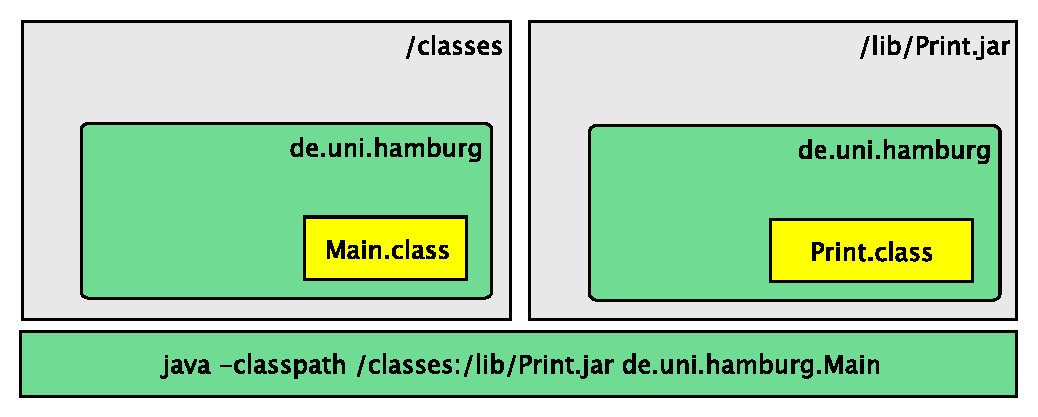
\includegraphics[width=\textwidth]{material/images/Classpath2.pdf}
    \caption{Java ClassPath}
    \label{fig:cps}
  \end{figure}

  % Klassenpfad Zusammensetzbar  
  Im Beispiel \ref{fig:cps} besteht der Klassenpfad aus einem Verzeichnis sowie einem JAR Archive, die für die Ausführung nötige Klassen umfassen. Da beide Orte eine Dateistruktur beinhalten, unterliegen sie einer Einschränkung: beide müssen die Paketstruktur der Java Klassen widerspiegeln, so dass der \textit{Applikation Klassenlader} diese durchsuchen kann. Abschließend braucht Java einen Startpunkt, mit dem die Applikation ihre Ausführung beginnt. 

  % Classloading mit Richtung 
  Beim Starten der Applikation werden Klassen instanziiert, indem der Klassenpfad, von links nach rechts, nach dem benötigten Typ durchsucht und diese erstellt. Somit hat der Klassenpfad eine interne Ordnung und eine Abarbeitungsreihenfolge. 

  \begin{figure}[h]
    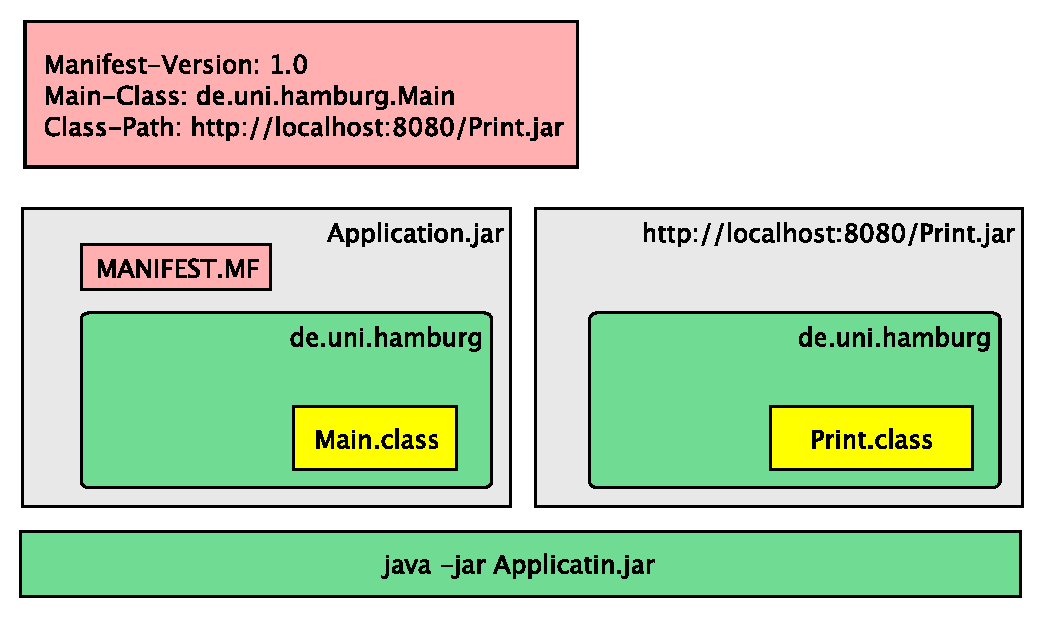
\includegraphics[width=\textwidth]{material/images/Classpath-Manifest2.pdf}
    \caption{Jar ClassPath}
    \label{fig:cpa}
  \end{figure}

  % Erweitere Klassenpfad mit dem Manifest 
  Im Beispiel \ref{fig:cps} wurde explizit ein Applikationsklassenpfad gesetzt, der für die Ausführung benötigten Klassen zuständig ist. Für den Ablauf großer Applikationen mit viele Abhängigkeiten kann dieser ausgedehnt und chaotisch werden. Von daher bietet Java eine Archivstruktur, die einen standardisierten Aufbau sowie zusätzliche Meta-Information über den Container in sich trägt. 
  
  % Manifest Meta-information 
  Dank der Java Strukturrichtlinie, befindet sich der komplette Inhalt eines Archivs auf dem Applikationsklassenpfad und kann zusätzlich in der \textit{manifest.mf} Datei erweitert werden. Die \textit{manifest.mf} spielt eine große Rolle in der Entwicklung von Java Applikation, diese kann den Namen, die Version, den Entwickler und die Sicherheitsattribute tragen, die während der Laufzeit ausgewertet werden können. Zum Beispiel wird in \ref{fig:cpa} der Klassenpfad durch ein Archiv aus dem Web erweitert und für die Ausführung genutzt. Des Weiteren hält die \textit{manifest.mf} einen Einstiegspunkt für die Ausführung, der auf eine Klasse mit der \textit{main} Methode verweist.\newline
  Somit kann die Applikation in einer kurzen und einfachen Form gestartet werden, da der Ausführungskontext durch die Struktur und die mitgelieferte Meta-Information komplett ist. \cite{classLoadingOracle}


\section{Klassenlader}\label{sec:cl}

  % Aufteilung der Verantwortung 
  In den vorherigen Beispielen [\ref{fig:cps}, \ref{fig:cpa}] wurde die Bedeutung und die Rolle des Klassenpfads für die Applikation beschrieben, dennoch muss dieser zuerst verarbeitet werden. Diese Aufgabe wird von dem Klassenlader übernommen, der eine zentrale Rolle in jeder Applikation spielt, weil er nach benötigten Java Klassen für die Instanziierung der entsprechenden Typen sucht. Da es eine wichtige Aufgabe ist, wird die Verantwortung für das Laden der Klassen über eine Menge von Klassenlader aus dem \textit{Klassenlader-System} aufgeteilt. 


  \subsection{Klassenlader-System} \label{sec:cls}

    % Gründe 
    Das \textit{Klassenlader-System} besteht aus drei integrierten Klassenlader, von denen jeder einen anderen Gültigkeitsbereich für das Laden der Klassen besitzt. Beim Abstieg der Hierarchie wird der Umfang der verfügbaren Quellen breiter und weniger vertrauenswürdig. 

    \begin{figure}[h!]
      \centering
      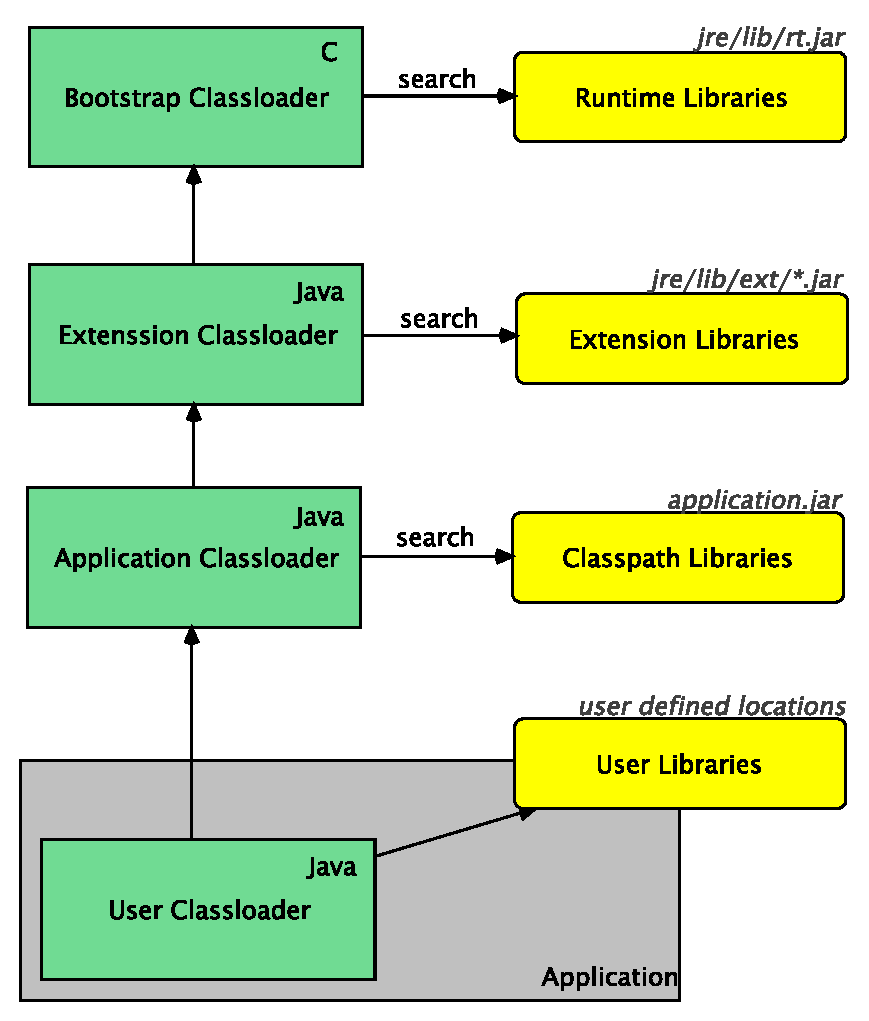
\includegraphics[width=0.7\textwidth]{material/images/Classloader-Hierarhie2.pdf}
      \caption{Klassenlader-System \cite{classLoadingIntro}}
      \label{fig:cl}
    \end{figure}
    
    % Aufbau
    Oben in der Hierarchie befindet sich der \textit{Bootstrap-Klassenlader}. Dieser Klassenlader ist verantwortlich für das Laden der grundlegenden Java Klassenbibliothek, wie zum Beispiel Java-Core-API aus der \textit{rt.jar}. Diese Klassen sind am vertrauenswürdigsten und werden zum Starten der virtuellen Maschine verwendet. Der Klassenlader für Erweiterungen kann Klassen  aus dem Standarderweiterungspaket im Erweiterungsverzeichnis \textit{lib/ext} dazu laden. Diese können Java-UI wie kryptografische Erweiterungen beinhalten. Der darunterliegende \textit{Applikation Klassenlader} ist zuständig für unseren Code und lädt Klassen aus dem allgemeinen Klassenpfad einschließlich der zu startenden Anwendung. Zuletzt können benutzerdefinierte Klassenlader erstellt werden, die sich auf der unteren Ebene der Klassenlader-Hierarchie befinden und auf Drittanbieter Bibliotheken zugreifen können. Demzufolge sind diese Quellen nicht sicher genug, um eine große Priorität zuzuweisen, wie zum Beispiel den geladenen Klassen des \textit{Bootstrap-Klassenlader}.\bigbreak 
    % Delegierungsmodell übergang
    Das in \ref{fig:cl} abgebildete Klassenlader-System verhindert, dass der Code aus weniger sicheren Quellen vertrauenswürdige Core-API-Klassen ersetzt, indem derselbe Name als Teil der Core-API angenommen wird. Daraus folgt ein Delegierungsmodell, welches eindeutige Klassen garantiert, da die Klassensuche von Oben nach Unten der Klassenlader-Hierarchie abgearbeitet wird.  \cite{classLoadingIntro} 
    

  \subsection{Delegierungsmodell} \label{sec:dm}
    
    % Suchalgorithmus  
    Das \textit{Klassenlader-System} delegiert jede Anfrage zum Laden einer bestimmten Klasse zuerst an seinen übergeordneten Klassenlader, bevor der angeforderte Klassenlader versucht die Klasse selbst zu laden. Jeder Klassenlader hält somit einen Verweis auf einen übergeordneten Klassenlader und ist Teil eines Klassenlader Baums mit dem \textit{Bootstrap-Klassenlader} an der Wurzel. 

    % Rekursiv 
    Wenn eine Instanz einer bestimmten Klasse benötigt wird, prüft der Klassenlader, der die Anfrage bearbeitet, normalerweise mit seinem übergeordneten Klassenlader vorab. Der übergeordnete Klassenlader durchläuft wiederum den gleichen Prozess bis die Delegierungskette den \textit{Bootstrap-Klassenlader} erreicht. Sobald der \textit{Bootstrap-Klassenlader} erreicht wurde, beginnt die tatsächliche Suche nach der gewünschten Klasse.

    \begin{figure}[h]
      \centering
      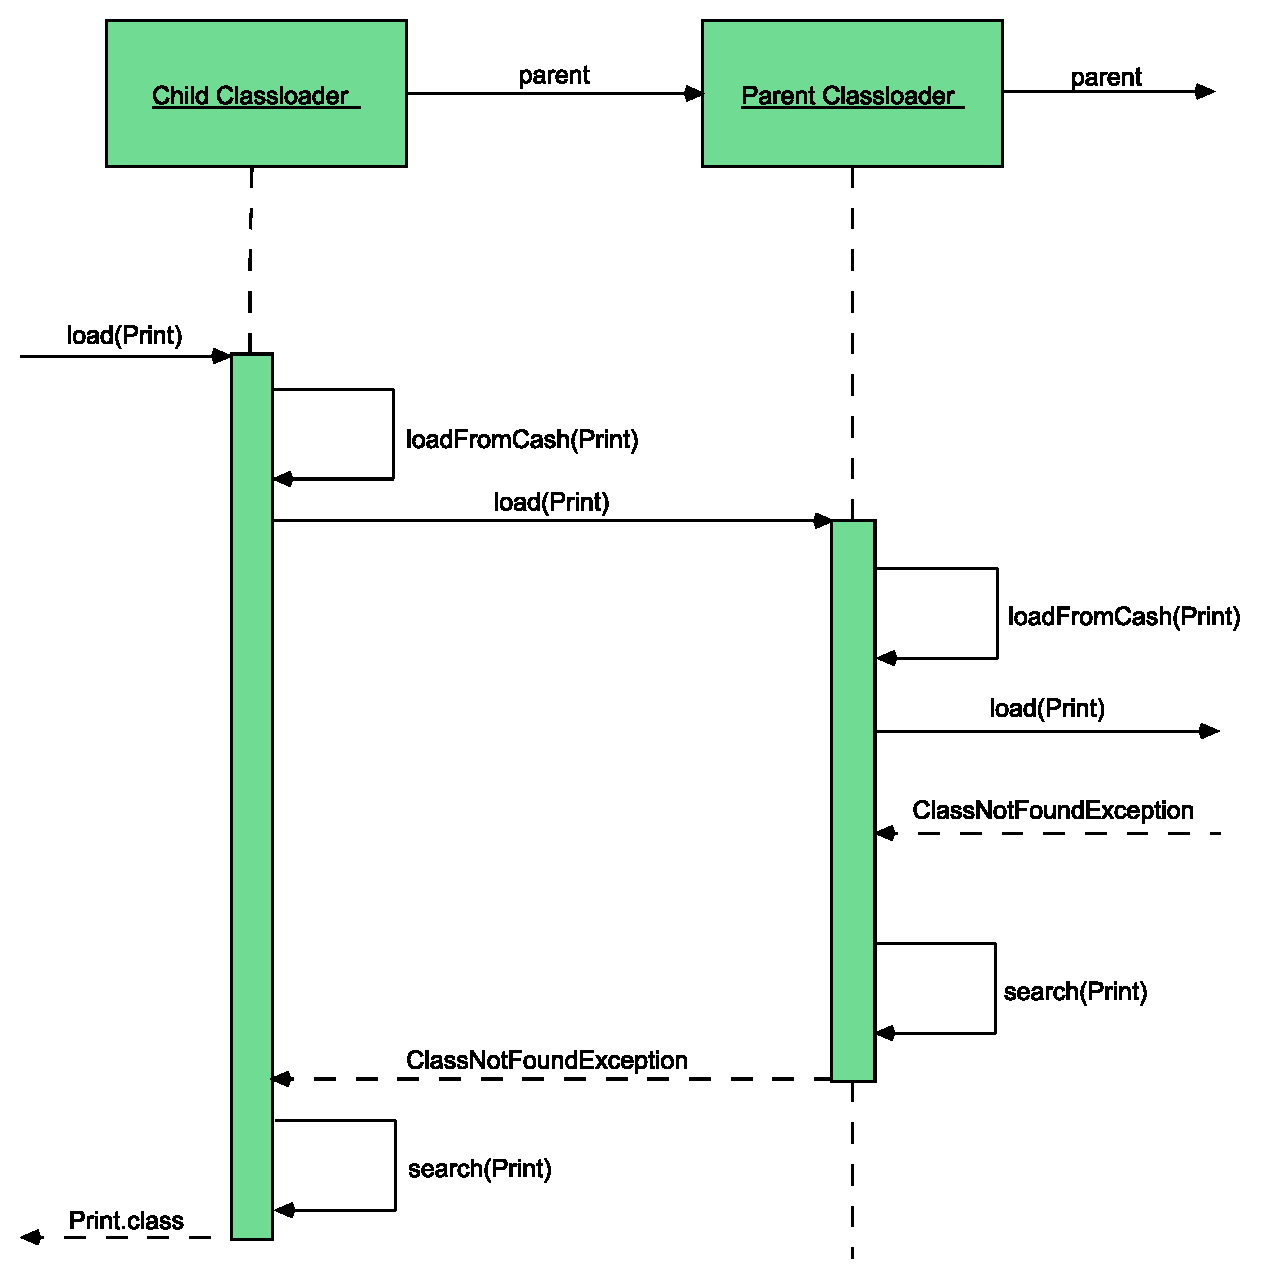
\includegraphics[width=0.9\textwidth]{material/images/flussCL.pdf}
      \caption{Klassensuche \cite{Forman04javareflection}}
      \label{fig:deligation}
    \end{figure}

    % Sichtbarkeit und Hierarchie 
    Wenn während der Suche ein übergeordneter Knoten eine bestimmte Klasse findet, dann wird diese Klasse die Baumhierarchie herunter zu der Anfrage delegiert. Andernfalls versucht der zuständige Klassenlader als letzter die Klasse selbstständig zu laden. Dies bedeutet, dass eine Klasse normalerweise nicht nur in dem Klassenlader sichtbar ist, der sie geladen hat, sondern auch für alle untergeordneten Instanzen. Dies bedeutet auch, wenn eine Klasse von mehr als einem Klassenlader in einem Baum geladen werden kann, wird immer die Klasse des übergeordneten Klassenlader eingelesen priorisiert. Dennoch wird vor jedem Laden der Klasse der Cash-Speicher des Klassenladers nach der gewünschten Instanz durchsucht. Wenn diese existiert, wurde die Suche bereits zuvor durchgeführt und keiner der übergeordneten Klassenlader außer dem jetzigen war fähig die Anfrage zu beantworten. Somit kann die Suche beschleunigt werden, indem der Typ sofort zurückgegeben wird. \cite{parentDelegationModel}


  \subsection{Namensräume} \label{sec:nam}

    Geladene Klassen werden sowohl durch den Klassennamen als auch durch den Klassenlader eindeutig identifiziert. Demzufolge werden geladene Klassen in \textit{Namensräume} unterteilt, die vom \textit{Klassenlader-System} individuell behandelt werden \cite{namespaces}. 

    % Idee 
    Ein \textit{Namensraum} ist eine Gruppe von Klassennamen, die von einem bestimmten Klassenlader geladen worden sind. Wenn ein Eintrag für eine Klasse einem \textit{Namensraum} hinzugefügt wurde, ist es nicht möglich, eine andere Klasse mit demselben Namen und unterschiedlichen Inhalt in den gleichen \textit{Namensraum} einzubinden. Nichtsdestotrotz können mehrere Kopien einer beliebigen Klasse in die Applikation geladen werden, indem für jede Klasse ein Klassenlader mit dem separaten \textit{Namensraum} erstellt wird \cite{customClDiffSpace}. 

    \begin{figure}[h]
      \centering
      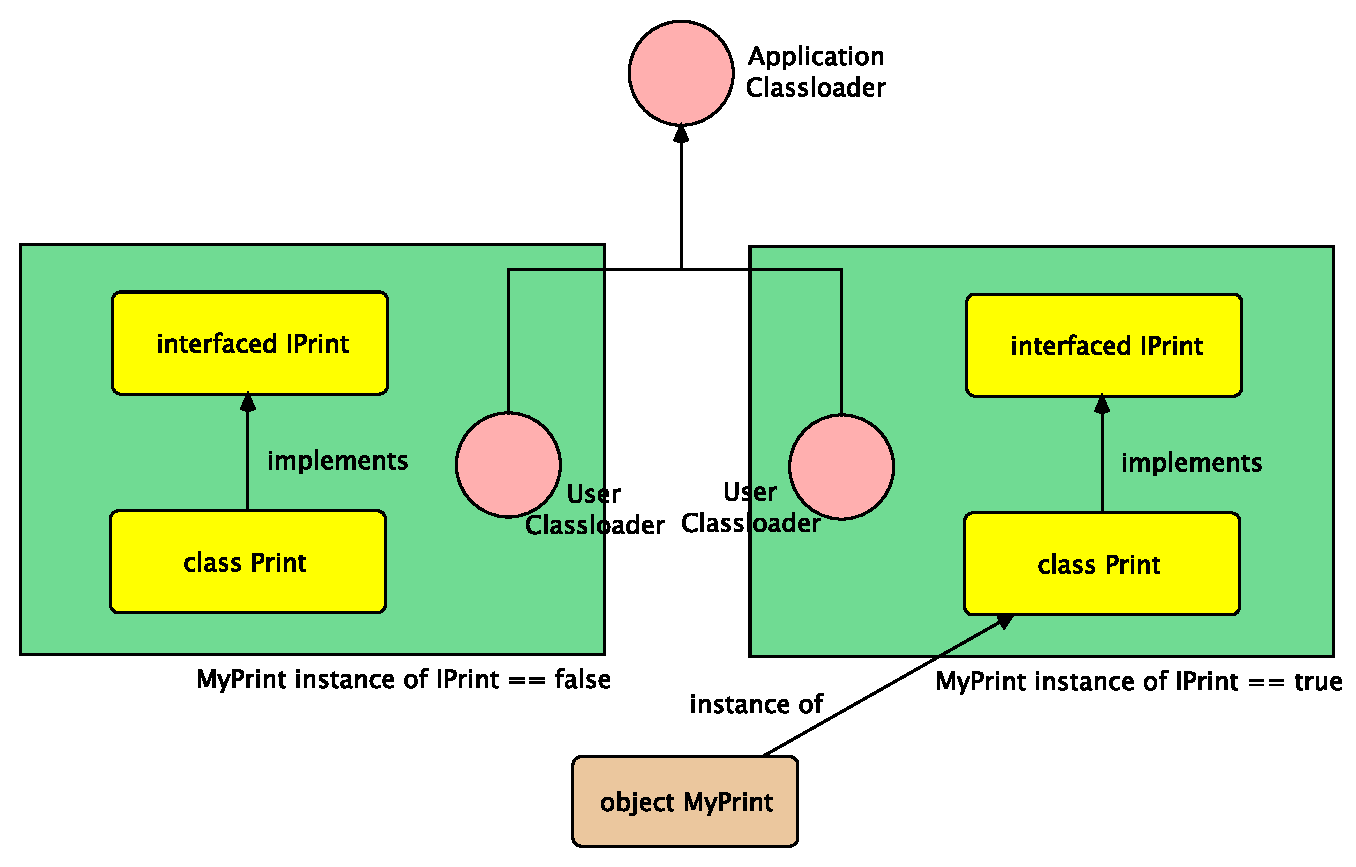
\includegraphics[width=0.9\textwidth]{material/images/namespace.pdf}
      \caption{Namensräume \cite{customClDiffSpace}}
      \label{fig:nam}
    \end{figure}

    % Ungleichheit identischer Klassen 
    Die Abbildung \ref{fig:nam} zeigt ein Beispiel für eine Klassenidentitätskrise, die sich ergibt, wenn eine Schnittstelle und die zugehörige Implementierung jeweils von zwei separaten Klassenlader geladen werden. Obwohl die Namen und binären Implementierungen der Schnittstellen und Klassen gleich sind, kann eine Instanz der Klasse von einem Klassenlader nicht als Implementierung des Interfaces von dem anderen Klassenlader erkannt werden. Bei Wunsch kann dieser Umstand gelöst werden, indem das Interface eine Ebene höher rutscht und von den Applikation Klassenlader geladen wird. Somit implementieren beide \textit{Print} Klassen dieselbe Schnittstelle.\bigbreak 

    % Schutz des Codes 
    Der Klassen Namensraum bietet zusätzliche Sicherheitsfunktionen wie die Kapselung privat deklarierter Pakete. Denn die Namensräume verhindern, dass der weniger vertrauenswürdige Code, der aus der Applikation oder benutzerdefinierte Klassenlader geladen worden ist, direkt mit mehr vertrauenswürdigen Klassen interagieren kann. Beispielsweise wird die Kern-API vom \textit{Bootstrap-Klassenlader} geladen, diese kann \textit{package private} Code enthalten, der bei Anfrage nicht an die unterliegende Klassenlader weitergereicht wird.


    % Schutz der privaten Pakete 
    Auch wenn ein untergeordneter Klassenlader die Paketstruktur der Core-API nachahmt, wird diese nicht als Teil der Java Core-API anerkannt, da dieser von den falschen Klassenlader geladen wurde. Somit verhindert die Verwendung von Namensräumen die Möglichkeit spezielle Zugriffsberechtigungen auf private Pakete zu erhalten, indem man selbst geschriebenen Code diesen zuweist. \cite{Forman04javareflection}


\section{Schnittstellen} \label{sec:kap}
  
  % Funktion 
  Die Schnittstelle und dessen Implementierung spielt eine entscheide Rolle für das Nutzen der Klassenfähigkeit. Eine Schnittstelle ist ein Vertrag, die die Funktionalität aller Klassen, die dieses implementieren beschreibt. Wenn eine Klasse eine bestimmte Schnittstelle implementiert, verspricht sie die Umsetzung aller in der Schnittstelle deklarierten Methoden.

  \begin{figure}[h!]
    \centering
    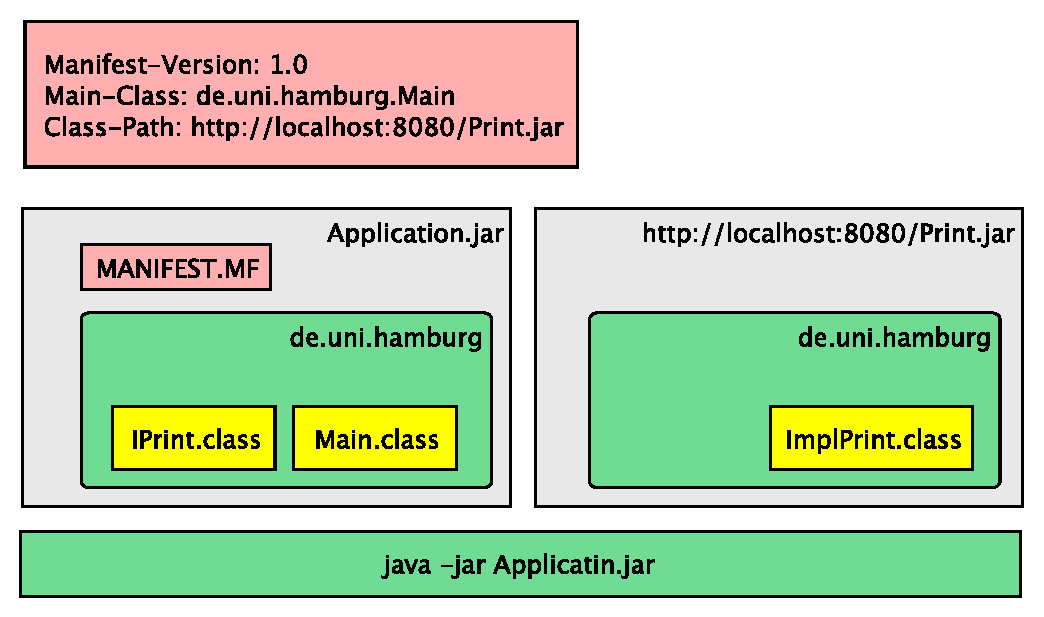
\includegraphics[width=0.8\textwidth]{material/images/Classpath-Interface-Implimentation.pdf}
    \caption{Schnittstelle}
    \label{fig:schnitt}
  \end{figure}

  % ist ein Garantie
  Somit wird durch die eigene Umsetzung des Schnittstellenvertrags ein mögliches Verhalten für die Nutzer der Schnittstellenbeschreibung implementiert. Daraus folgt ein Kommunikationsvertrag zwischen zwei Objekten, denn wenn eine Klasse eine Schnittstelle implementiert, implementiert diese alle in dieser Schnittstelle deklarierten Methoden und der Methodenaufruf an dieser Klasse wird garantiert ausgeführt.\cite{bloch2017effective}\bigbreak 
  
  % Dynamische Klassenbindung 
  Im Beispiel \ref{fig:schnitt} wird der Vorteil des Schnittstellenvertrags demonstriert, der das Ausführen der unbekannten \textit{PrintImpl} Umsetzung, durch eine einfache Schnittstellenbeschreibung \textit{IPrint} garantiert. Solange die Implementation sich auf derselben Klassenpfadhierarchie befindet wie die Schnittstelle, wird diese während der Laufzeit auf Kompatibilität geprüft und angewandt. Somit können dynamische Klassenbindungen während der Laufzeit entstehen und Laufzeitbibliotheken ausgetauscht werden, ohne dass die Applikation verändert wird. Hätte man die Schnittstelle nicht genutzt, würde man die Implementation nur als ein Objekt Type instanziieren können und hätte keinen einfachen Zugriff auf ihre Methoden. In der Konsequenz verbirgt die Schnittstelle ihre Implementierungsdetails der Methoden und gewährt den Vertragspartner keinen Einblick in ihre Umsetzung. Daraus folgt eine einfache Ersetzbarkeit der Implementationsvertreter, ohne den Klienten anpassen zu müssen. \cite{Forman04javareflection}

\section{Reflektion}\label{sec:refl}
  % Kurze einleitung 
  Reflektion ist die Fähigkeit eines laufenden Programms, sich selbst und seine Softwareumgebung zu analysieren und zu ändern. 
  Somit hat die Applikation eine Möglichkeit, durch Reflexion, die Information über ihre Struktur und ihr Verhalten zu erhalten, um wichtige Entscheidungen zu treffen. Je nachdem welche Information durch die Untersuchung eigener Klassen ausgelesen wurde, können Objekte, die während der Kompilierung nicht präsent waren, mithilfe der Reflektion-API während der Laufzeit instanziiert, bearbeitet und genutzt werden. Somit ermöglicht Reflektion das Arbeiten mit Klassen, von denen man im Voraus nicht wissen kann, wie zum Beispiel von Klassen, die in der Zeit nach der Applikation entstanden sind.\bigbreak 
 % Überblick: Problemstellung die Reflexion löst 
  In vielen Fällen der Applikationsentwicklung möchte man die Applikation von anderen Nutzern und Entwicklern erweitern lassen, ohne dass diese bei jeder Änderung die komplette Applikation umbauen müssen. Somit stellt sich die Frage, wie erstellt man ein Mechanismus, der mit beliebigen Klassen arbeiten kann.\newline
  Man könnte mit den zuvor vorgestellten Schnittstellen- und Implementierungsansatz eine gemeinsame Schnittstelle für Erweiterungen definieren, die unserer Applikation mit einer Implementation erweitern lässt und die entsprechenden Methoden definiert. Nichtsdestotrotz besteht die Applikation nicht nur aus unserem Code, sondern zusätzlich aus dem Kern und Drittanbieter Bibliotheken, über die wir keine Kontrolle verfügen. Somit ist die Erweiterung der gesamten Codebasis mit der entsprechenden Schnittstelle oder eine Verschachtelung von \textit{instanceof} Blöcken keine simple oder saubere Lösung. Dementsprechend sollte Reflektion genutzt werden. Diese ermöglicht den Einblick in die Klassenstruktur, ohne direkten den Typen zu kennen. Die Klassenstruktur enthalten Informationen über die Klasse selbst, zum Beispiel das Paket, die Superklasse der Klasse sowie die von der Klasse implementierten Schnittstellen. Es enthält auch Details zu den von der Klasse definierten Konstruktoren, Feldern und Methoden.\bigbreak

  \begin{figure}[h!]
    \centering
    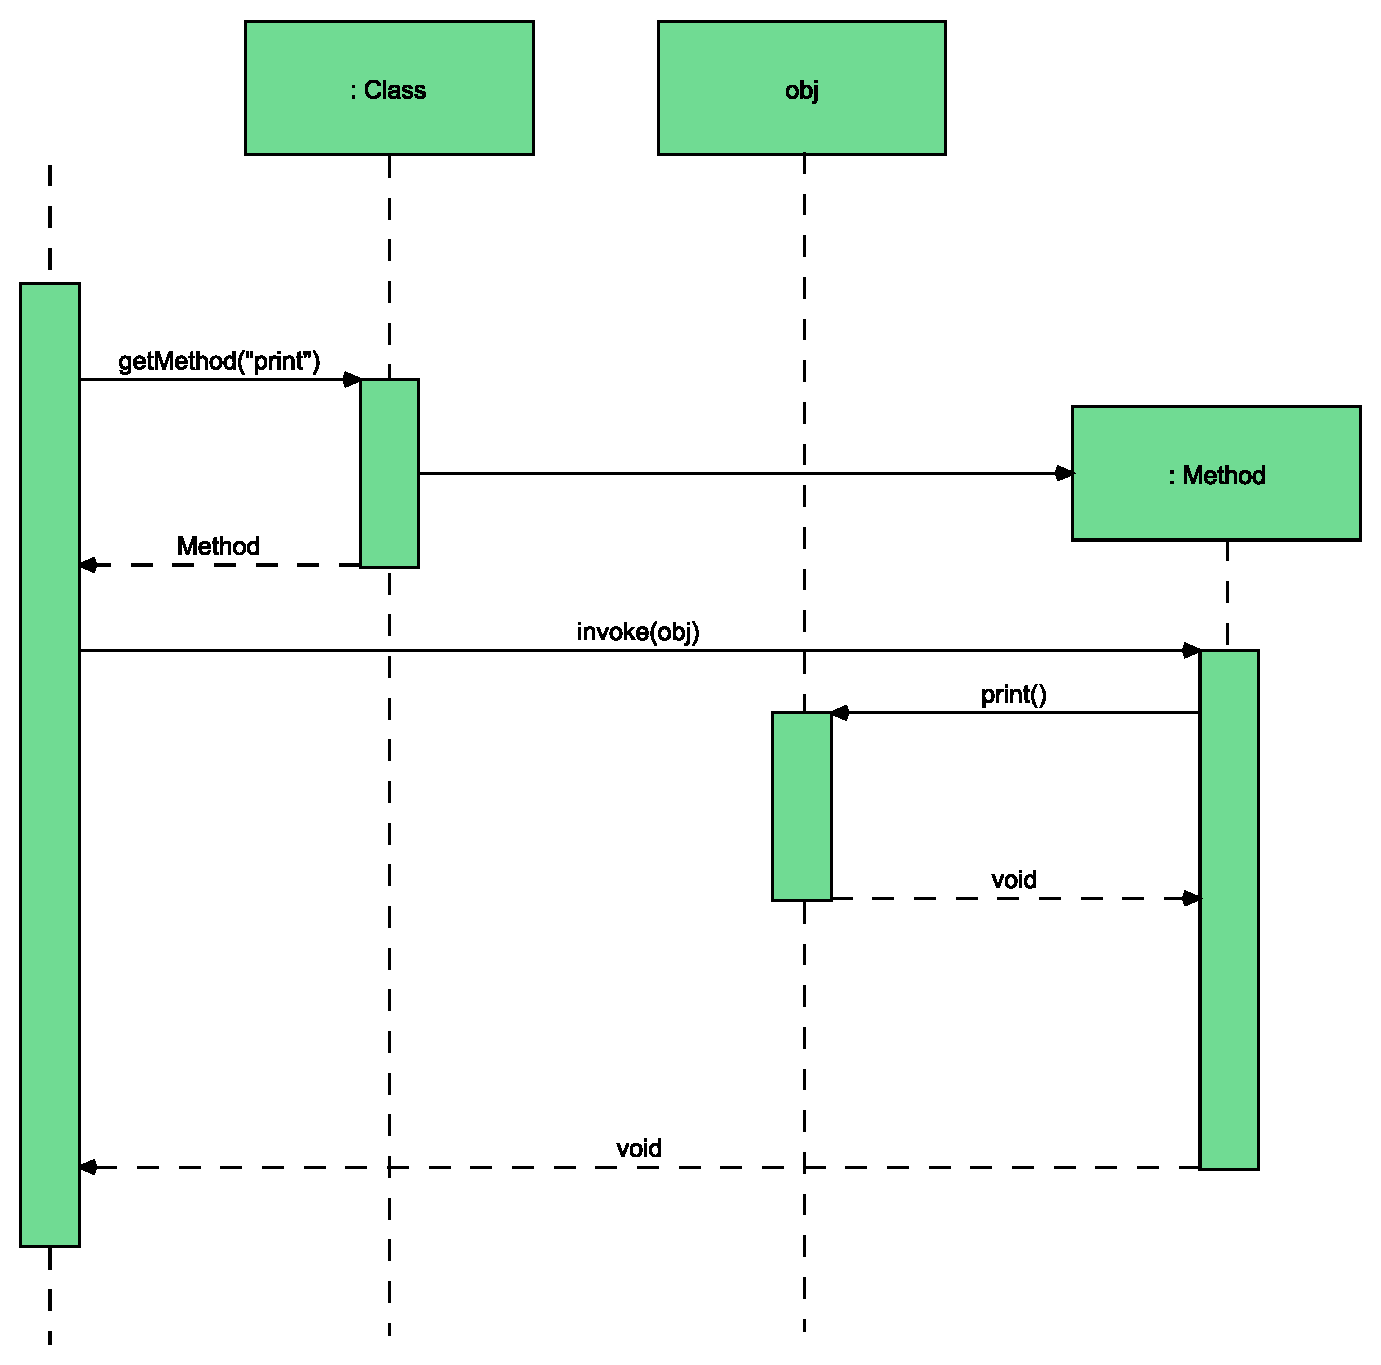
\includegraphics[width=0.8\textwidth]{material/images/flussReflection.pdf}
    \caption{Aufruf einer Methode \cite{Forman04javareflection}}
    \label{fig:refl-fluss}
  \end{figure}

  % Sequenzdiagram 
  In der Abbildung \ref{fig:refl-fluss} wird ein Ablauf eines Methodenaufrufs mithilfe von Reflektion visualisiert. Im ersten Schritt muss die Methode gefunden werden. Da wir den Typen nicht kennen und nur für den Stammobjekt Typen deklarieren Methoden nutzen können, lassen wir das Objekt sich selbst inspizieren und die geforderte Methode finden. Dafür wird nach einer bestimmten Methode der Klasse gesucht und bei Erfolg ein Objekt von Typ \textit{Method} zurückgegeben. Das Methodenobjekt enthält die ganze Information über die gesuchte Methode, wie zum Beispiel Parameter und Rückgabewerte. Ausgerüstet mit der benötigten Information kann die Methode ausgeführt werden. Dafür braucht das Methodenobjekt eine Instanz der passenden Klasse sowie für die Ausführung benötigten Parameter. Nach der Abwickelung wird das Ergebnis der Ausführung vom der Objektinstanz über das Methodenobjekt zurück in den Programmfluss delegiert. \cite{Forman04javareflection} 

 % Nutzen: Felder Methode, Konstruktoren
  \bigbreak Somit sind die drei Hauptmerkmale einer Klasse ihre Felder, Methoden sowie Konstruktoren durch eine entsprechendes Java Objekt aus der Reflektion-API repräsentiert. 

  \begin{itemize}
    \item java.lang.reflect.Field
    \item java.lang.reflect.Method
    \item java.lang.reflect.Constructor
  \end{itemize}

  Mithilfe des Klassen Typs können die oben genannten Objekte erzeugt und manipuliert werden. Diese bieten Schnittstellen für das Abfragen der Klassenstruktur an und repräsentieren Charakteristika der entsprechenden Klassen.

  \begin{itemize}
    \item Field[ ] *.class.getFields();
    \item Method[ ] *.class.getDeclaredMethods();
    \item Constructor[ ] *.class.getConstructors();
  \end{itemize}
  \bigbreak 

  Um den Zusammenhang und den Nutzen von Reflektion darzustellen, wird in der Abbildung \ref{my-refl} ein Szenario durchgespielt, das eine unbekannten Typen mithilfe des Konstruktors initialisiert, dessen Methoden aufruft, das Feld bearbeitet und wiedergibt, ohne die Objektstruktur im Voraus zu kennen. Des Weiteren ist zu beachten, dass statische Klassenmethoden sowie private Felder und Methoden mithilfe von Reflektion offen zugänglich gemacht werden können.\cite{Forman04javareflection}\bigbreak 

  % Bild mit Code der eine Objekt erstellt und Methoden aufruft. Mit Kommentaren zwischen den Zeilen.
  \begin{lstlisting}[caption=Reflektion in Aktion,label=my-refl,captionpos=b]
    public static void getMethods(@NotNull Class clazz) throws
            NoSuchMethodException, NoSuchFieldException,
           InvocationTargetException, InstantiationException,
           IllegalAccessException {
      Method method;

        // Instantiierung
        Constructor[] ctors = clazz.getDeclaredConstructors();
        Object dynamic = ctors[0].newInstance(4);
        // Aufruf einer privaten Methode
        method = clazz.getDeclaredMethod("print", String.class);
        method.setAccessible(true);
        method.invoke(dynamic,"Hello World");
        // Feld Manipulation
        Field field = clazz.getDeclaredField("version");
        field.set(dynamic, 5);
        int version = (int) field.get(dynamic);
        System.out.println(version);
    }
  \end{lstlisting}

 % Wo wird Reflektion genutzt, wieso ist es so nützlich in der Modernen Software-Entwicklung 
  Wie in der Abbildung \ref{my-refl} dargestellt ist Reflektion ein mächtiges Werkzeug, das aus der morden Softwareentwicklung nicht wegzudenken ist und wird in zahlreichen Framework's verwendet, um den Entwickler zu unterstützen. 

  \begin{itemize}
    \item Zum Beispiel wird \textit{Dependency Injection} mithilfe von Reflektion realisiert, indem ein Framework, wie zum Beispiel Spring, die entsprechende Implementierung für ein Interface sucht und initiiert. In Diesem Zusammenhang wird Anhand des \textit{implement} Schlüssels und zusätzlicher Meta-Information aus der Klassen \textit{Annotation} ein eindeutiger Kandidat auserwählt und konstruiert.
    \item Beim Serialisieren und Deserialisieren von Objekten werden die Objektfelder in JSON und wieder zurück konvertiert, ohne die Feldnamen sowie ihre Anzahl zu kennen.
    \item Die Web-Container Tomcat oder WildFly leiteten die Web-Anfragen an das entsprechende Modul durch das Analysieren der \textit{web.xml} und Anfordern der passenden URI.
    \item JUnit verwendet Reflektion, um die Methoden einer Klasse nach Test-Annotation zu durchsuchen, um diesen anschließend aufzurufen.
  \end{itemize}

\section{Gradle}
Gradle ist ein Build-Tool ähnlich wie Maven und Ant. Gradle ist das neueste dieser drei Build-Tools, und wird zunehmend eingesetzt. Es ist Open Source und hat viel Akzeptanz bei den Entwicklern gefunden, da es auf die Erfahrung aus den vorhandenen genannten Build-Tools zurückgreift. Mehrere bekannte Projekte wie Android, Spring Framework und Hibernate haben ihre Build-Systeme bereits auf Gradle migriert. Einige der Vorteile, die Gradle gegenüber Maven und Ant hat, sind präzisere Erstellungsskripte und eine flexiblere Erstellungssprache.\bigbreak

\subsection{Beweggründe für Gradle}
Für die Migration von Ant auf Gradle werden im Folgenden die Schwächen von Ant gegenüber Gradle aufgelistet.
\begin{itemize}
  \item Die Verwendung von XML als Definitionssprache für die Erstellungslogik führt zu übermäßig großen und ausführlichen Erstellungsskripten im Vergleich zu Erstellungswerkzeugen mit einer prägnanteren Definitionssprache. \cite{muschko2014gradle}
  \item Komplexe Erstellungslogik führt zu langen und nicht verwaltbaren Erstellungsskripten. Der Versuch, bedingte Logik wie \textit{if-then}, \textit{for-each} oder \textit{while} Anweisungen mit XML zu definieren, wirkt unnatürlich und aufgeblasen.\cite{muschko2014gradle}
  \item Ant gibt keine Richtlinien zum Einrichten des Projekts. In einem Unternehmen führt dies häufig zu einer Build-Datei, die jedes Mal anders aussieht.\cite{berglund2011building}
  \item Gemeinsame Funktionen werden häufig kopiert und eingefügt. Jeder neue Entwickler im Projekt muss die individuelle Struktur eines Builds verstehen.\cite{varanasi2015introducing}
  \item Die Verwendung von Ant ohne Ivy erschwert das Verwalten von Abhängigkeiten. In vielen Fällen müssen die JAR-Dateien in die Versionskontrolle eincheckt und deren Organisation manuell verwaltet werden.\cite{varanasi2015introducing}
\end{itemize}

\subsection{Aufbau der Umgebung}
  Die gradle Umgebung besteht aus mehreren Komponenten. Jede von den Komponenten wird in einem bestimmten Lebenszyklus von Gradle für das Erstellen der Applikation genutzt.\newline
  Um Gradle zu starten, werden zwei ausführbare Skripte mitgeliefert. Für die Ausführung auf dem \textit{Unix} basierte Systeme kann \textit{gradlew} verwendet werden und für die Windows Ausführung ist das \textit{gradlew.bat} Skript zuständig.\bigbreak
  \begin{figure}[h!]
    \centering
    \begin{minipage}{7cm}
      \dirtree{%
       .1 .
       .1 build.gradle.
       .1 gradle.
       .2 wrapper.
       .3 gradle-wrapper.jar.
       .3 gradle-wrapper.properties.
       .1 gradlew.
       .1 gradlew.bat.
       .1 settings.gradle.
       }
    \end{minipage}
    \caption{Gradle Konfiguration \cite{gradleStructure}}
    \label{fig:gradle_project_structure}
  \end{figure}

  Nach dem Anstoßen des Ausführung Skripts, wird Gradle konfiguriert und setzt eine bestimmte Zielversion für die Ausführung fest. Dies geschieht innerhalb der \textit{gradle/wrapper} Ordnerstruktur und initiiert Gradle für die Ausführung. Als nächstes sammelt Gradle die Information über alle Teilnehmer der Projektorganisation und legt eine globale Projektstruktur für die Ausführung fest. Dafür wird in der Initialisierungsphase die \textit{settings.gradle} der Projekte und die Lokale \textit{init.gradle} Konfigurationsdatei ausgelesen. Diese bestimmen Umgebungsvariablen, Eigenschaften und persönlichen Informationen. Des Weiteren werden teilnehmende Projekte gesetzt und instanziiert.\newline
  Nachdem die Initialisierungsphase beendet ist, werden erstellte Projekte konfiguriert. Die Konfiguration geschieht laut den \textit{build.gradle} Konfigurationsdatei und bereitet die Projekte für die Ausführung vor. Zum Schluss wird das Bauen durchgeführt, indem eine Reihe von Ausführungsschritten (Tasks) von dem Nutzer aufgerufen werden.\cite{mitra2015mastering}


\subsection{Gradle build Skript}
\begin{lstlisting}[caption=Gradle in Aktion \cite{ikkink2015gradle},label=my-grl,captionpos=b]
  // Deklaration ders genutzten Plugins 
  plugins {
      id 'java'
  }
  // Bibliothek Quellen 
  repositories {
      mavenCentral()
  }
  //Projektbindung
  dependencies {
      compile('javax:javaee-web-api:8.0')
  }
  // Klassenpfade 
  configurations {
    libs
    plugins
    compile
  }
  // Felder
  group 'de.firm'
  description 'my first application'
  version version
  defaultTasks 'war'
  // Projektstruktur
  sourceSets {
      main {
          java {
              srcDirs ['src/main/java']
              webAppDirName 'src/main/webapp'
              outputDir file('out/classes')
          }
          resources {
              srcDirs ['src/main/resources']
              output.resourcesDir = file('out/resources')
          }
      }
  }
  // Konfiguration eines Abarbeitungsschritts
  task war {
      setGroup("gradle")
      setArchivesBaseName(name)
      webInf {
          into('classes') {
              from sourceSets.main.java.outputDir
              into('META-INF') {
                  from(sourceSets.main.resources.files) {
                      include("persistence.xml")
                  }

              }
          }
      }
      metaInf {
          from(sourceSets.main.resources) {
              include("import.sql")
          }
          manifest {
              attributes 'version': war_version
              attributes 'description': war_description
              attributes 'creator': war_creator
              attributes 'classifier': war_classifier
          }
      }
  }
  // Task Graph Manipulation 
  deploy.dependsOn(war)
\end{lstlisting}

In der Abbildung \ref{my-grl} ist eine Standard Struktur eines Gradle Build Skript abgebildet, die mit einem Java Plugin arbeitet und ein war Archiv erstellt. 

\chapter{Modularisierung}
% Kapitel über Module 
% \section{Modularisierung} \label{sec:modularisierung}
  Modularisierungsansätze finden sich so gut wie in jeder Software wieder, da es sich um ein grundlegendes Prinzip für die Beherrschung eines Systems handelt. Gerade in der Java-Welt wird seit jeher das Ideal der lose gekoppelten Systeme verfolgt. 
  Es generiert  Struktur in großen Softwareprojekten, indem das Gesamtprodukt in kleine, praktische Bestandteile zerlegt wird. 
  Die Entwicklung von kleinen Projekten mit übersichtlicher Codebasis ist einfach zu überblicken und braucht keine strukturelle Basis, um den Entwickler Architektur und Funktion darzustellen. Dennoch ist die Zukunft eines Projekts nicht immer eindeutig und kann mit de Zeit an Größe und Komplexität gewinnen. Mit der Größe des Projekt wächst auch der Geschäftskontext und damit die Zahl der beteiligten Personen. Diese repräsentieren verzwickte Wünsche und Ziele, die an einer Stelle im Projekt nicht sauber umsetzbar sind.
  Demzufolge ist die richtige Aufstellung eines Projektes von Grund auf eine zukunftssichere Entscheidung. 
  
  Ohne die Modularisierung werden Änderungen an großen Projekten mühselig und mit unerwarteten Nebeneffekten umgesetzt. 
  Sowohl das Bauen und Ausrollen des Projekts als auch der Betrieb der Applikation, ist eine lange und aufwendige Aufgabe, die mit jedem kleine Fehler die komplett Applikation Neustarten lässt oder das Ausrollen unterbricht. 
  Somit können kleine Fehler das ganze Produkt aus dem Gleichgewicht bringen.
  Aus diesem Grund sollen Module diese Probleme adressieren und die Applikation in autonome, kleine Einheiten aufteilen, die unabhängig von einander ihre Funktionalität anbieten.

  % Moduleigenschaften 
  \subsection{Ziele der Modularisierung}
    Die Modularisierung beschäftigt sich mit der Aufteilung eines Systems in Module, die Komplexität verringern, indem die einzelnen Module getrennt voneinander betrachtet und verstanden werden. Dies wiederum unterstützt die Wartbarkeit der einzelnen Module. Darüber hinaus vereinfachen die von der Modularität geforderten definierten Schnittstellen zwischen den Modulen die Erweiterbarkeit des Systems. Und die Rekombination von Modulen erlaubt die Erstellung von verschiedenen Varianten der Umsetzung. 
    
    Um die Aufgabe des Java Modularisierung zu verstehen, bedarf es eine Aufstellung von Zielen und Qualitäten den sich die Modularisierung stellt. Für JPMS sind diese eindeutig in der \textit{JSR 376} beschrieben und spezifizieren die Folgenden Qualitäten.

    \subsubsection{Kapselung}
      Die Kapselung beschreibt ein Kontrollmechanismus, der die internen Struktur eines Moduls verwaltet.
      Demzufolge hat das Modul die komplette Kontrolle über ihre interne Struktur und kennt die Zugriffsrechte ihrer Bestandsteile, indem das Modul die Zugriffsrechte ihrer inneren Struktur explizit deklariert.

    \subsubsection{Interoperabilität}
      Die Interoperabilität beschreibt die Kommunikationsfähigkeit der Software mit anderen diversen Systemen, unabhängig von ihrer Sprache oder Plattform mit der diese betrieben wird. 
      Darum bieten Module Schnittstellen an, mit denen sie Dienste anbieten und anfordern können.

    \subsubsection{Zusammensetzbarkeit}
      Aus der Interoperabilität geht die Zusammensetzbarkeit hervor.
      Diese Steht für die Wiederverwendbarkeit der in sich abgeschlossenen Module für unterschiedliche Zwecke in unterschiedlichen Systemen, indem man diese auf bestimmte Art und Weise kombiniert. 

    \subsubsection{Erweiterbarkeit}
     Die Erweiterbarkeit hilft den modularen und zusammengesetzten System ihre Funktionalität zu skalieren, indem die Software durch individuelle Einheiten ergänzt werden kann. 

    \subsubsection{Autonomie}
      Mit der Autonomie werden unnötige Abhängigkeiten aufgelöst und nur die nötige Funktionalität für die entsprechende Aufgabe in einem Modul abgelegt. 
      Somit können einzelne Module im Betrieb bleiben, auch dann wenn Teile des System nicht reagieren.

  % Modulaufbau 
  \subsection{Modulstruktur}
    Die zuvor aufgeführten Ziele der Modularisierung liefern bereits eine Idee davon, was für Anforderungen Module erfüllen müssen, um von einem Modul sprechen zu können. Primär erfüllt ein Modul einen abgeschlossenen Aufgabenbereich und beinhaltet die dafür nötigen öffentlichen sowie privaten Operationen und Datenfelder. Die Kommunikation eines Moduls mit anderen Modulen und der Außenwelt erfolgt über eindeutig spezifizierte Schnittstellen.

      \begin{figure}[h!]
        \centering
        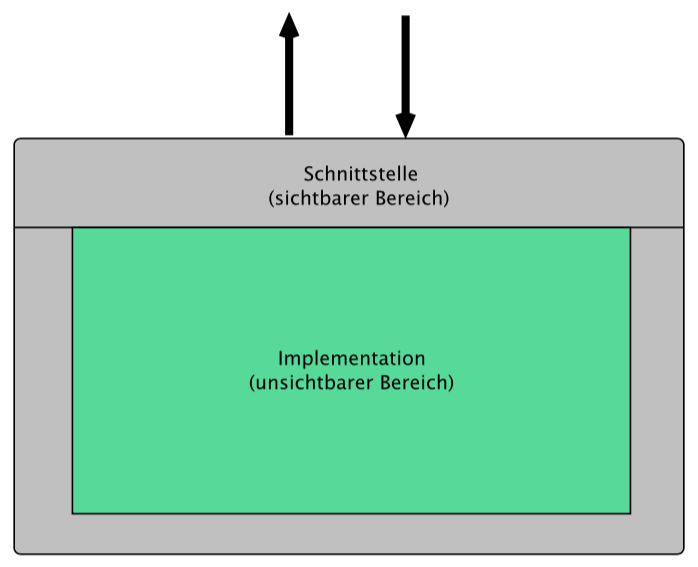
\includegraphics[width=0.6\textwidth]{material/images/simple-module.png}
        \caption{Simple Modulstruktur}
        \label{fig:simple-module}
      \end{figure} 

    Somit dient das Modul als ein Behälter für Objekte, der aus einem unsichtbaren und einem sichtbaren Bereich besteht. Der sichtbare Bereich ist die Schnittstelle des Moduls und ist die Aufzählung derer Objekte, die das Modul nach außen hin zur Verfügung stellt. Der Zugriff auf diese erfolgt über definierte Operationen in der Modulschnittstelle. Der unsichtbare Teil beherbergt die eigentliche Implementierung, also die umgesetzten Operationen und Daten.Unter diesen Umständen reduziert sich die Komplexität des Moduls für den Nutzer von der Gesamtimplementation auf die Schnittstellen. 

      \begin{figure}[h!]
        \centering
        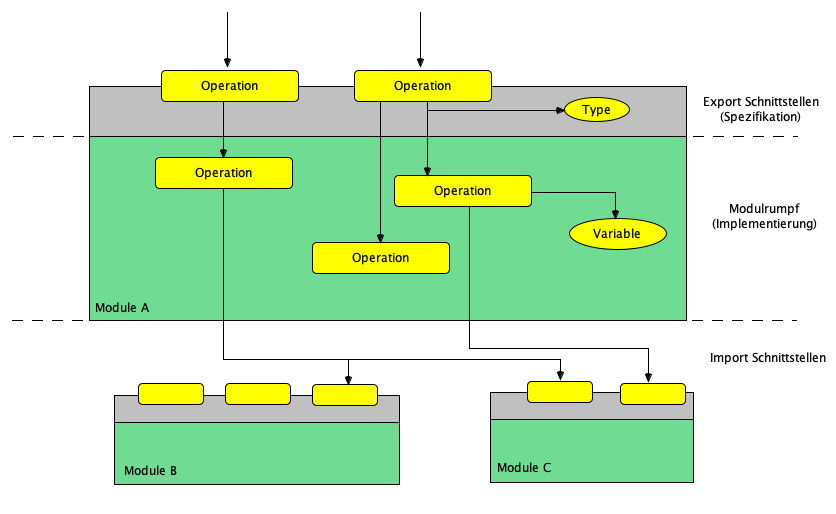
\includegraphics[width=\textwidth]{material/images/module-workflow.png}
        \caption{Schematischer Aufbau eines Moduls}
        \label{fig:module-workflow}
      \end{figure} 

    In der Abbildung \ref{fig:module-workflow} wird die interne Struktur sowie entsprechenden Verbindungen eines Moduls genau betrachtet. Zu sehen sind drei Module, die ihre Dienste mit dem \textit{exports} Schlüssel über die Schnittstellen anbieten und diese bei Bedarf mit anderen Modulen kombinieren können, indem weitere Funktionalität durch den \textit{requires} Schlüssel von zusätzlichen Modulen angefordert wird. Die interne Umsetzung der Funktionalität bleibt jedoch verborgen und kann Modulübergreifend nicht nachverfolgt werden. 

  % Moduldefenition schlussatz als zusammenfassung 
  \subsection{Moduleigenschaften}

\textbf{Modul Definition}
\begin{displayquote}
	\textit {'Ein Modul ist eine Sammlung von Algorithmen und Daten bzw. Datenstrukturen zur Bearbeitung einer in sich abgeschlossenen Aufgabe. Die Verwendung des Moduls (d.h. seine Integration in ein Programm-System) erfordert keine Kenntnis seines inneren Aufbaus und der konkreten Realisierung der gekapselten Algorithmen und Daten(-strukturen). Seine Korrektheit ist ohne Kenntnis seiner Einbettung in ein bestimmtes Programmsystem nachprüfbar.'} \cite{rechenberg2006informatik}
\end{displayquote}\bigbreak 

Aus dieser Definition ergeben sich folgende Eigenschaften, die ein Software-Modul beschreiben:

\begin{itemize}
  \item Zusammenfassung von Operationen und Daten zur Realisierung einer in sich abgeschlossenen Aufgabe 
  \item Kommunikation mit der Außenwelt nur über eine eindeutig spezifizierte Schnittstelle 
  \item Nutzung des Moduls möglich ohne Kenntnis des inneren Ablaufs 
  \item Die Struktur jedes Moduls sollte einfach genug sein, um vollständig verstanden zu werden.
  \item Anpassungen eines Moduls sollte ohne Kenntnis der Implementierung sowie ohne Einfluss auf das Verhalten anderer Module durchführbar sein.
  \item Korrektheit des Moduls durch Tests nachprüfbar ohne Kenntnis seiner Einbettung
  \item Wiederverwendbarkeit der Funktionalität im anderen Kontext
\end{itemize}

  % Wie modelliert man Module  
  \subsection{Modulentwurfskriterien}
    % Einleitung
    Nachdem die Struktur des Moduls klar bestimmt wurde, muss die Umsetzung einer Applikation mit Modulen auf Qualitätsmerkmale abgeglichen werden. Da die Aufteilung eines Entwurfsproblems in kleinere Teilprobleme nicht Selbstverständlich ist, kann diese mit verschieden Techniken und auf diverse Weise umgesetzt werden und bietet daher keine Garantie eines sauberen Entwurfs. Die Kunst Funktionalität in einem einzelnen Modul zu kapseln und diese mit geringer Abhängigkeit vom Restsystem betreiben zu können, kann mit Hilfe bestimmter Kriterien bewertet und angepasst werden. \bigbreak
    
    Bei der Modularisierung sind folgende Entwurfskriterien zu berücksichtigen: 
    \begin{itemize}
      \item Modulgeschlossenheit 
      \item Maximale Modulbindung 
      \item Minimale Modulkopplung 
      \item Minimale Schnittstelle 
      \item Modulanzahl 
      \item Modulgröße 
      \item Testbarkeit 
      \item Seiteneffektfreiheit 
      \item Importzahl 
      \item Modulhierarchie 
    \end{itemize}
    Mit Hilfe der \textit{Modulgeschlossenheit} wird die Abhängigkeit des Moduls von anderen Modulen reduziert und lässt diese separat bearbeiten und austauschen. Somit kapselt ein Modul eine bestimmte Funktionalität, die von Anfang bis zum Ende intern verarbeitet werden kann. Direkt daraus folgt im besten Fall eine \textit{maximale Bindung} oder starker Zusammenhang innerhalb eines Moduls, indem die internen Komponenten bestens mit einander verzahnt sind und sich gemeinsam mit eine gezielten Aufgabe beschäftigen. In der Konsequenz entsteht ein eingeschränkter Wartungsraum für Entwickler, die sich mit der entsprechenden Funktion beschäftigen. Um die Bindung der Komponenten innerhalb eines Moduls zu messen, können die Abhängigkeiten in verschieden Kategorien eingeteilt werden: Logisch, Zeitlich, Prozedural, Sequentiell, Informal und Funktional.

    \begin{figure}[h]
      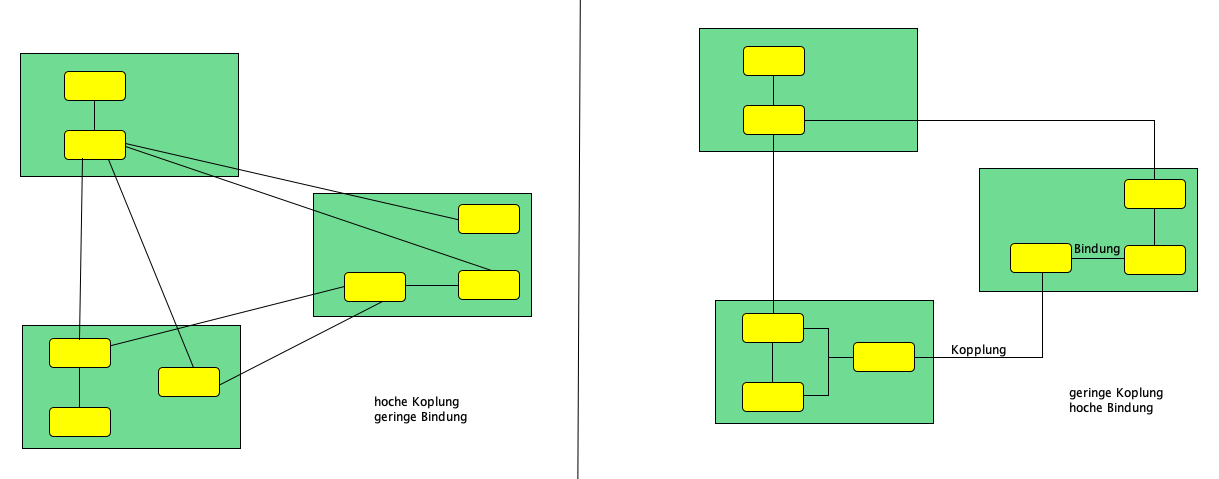
\includegraphics[width=\textwidth]{material/images/kopplung.png}
      \caption{Modulbindung und Modulkopplung}
      \label{fig:kopplung}
    \end{figure}

    Komplementär zu der \textit{maximale Bindung} beschreibt die \textit{minimale Kopplung} die Anzahl der Verbindung zwischen den Modulen. Diese sollte natürlich klein gehalten werden, um die Abhängigkeit zu reduzieren. Die \textit{minimale Kopplung} hat somit einen direkten und positiven Einfluss auf die Anzahl der Schnittstellen, indem diese übersichtlich und eindeutig die Funktion des Moduls beschreiben. Andernfalls kann eine starke Kopplung die Komplexität heben und Fehler begünstigen, indem der Umfang an Daten, die zwischen den Modulen ausgetauscht werden, erhöht wird. Eine \textit{minimale Kopplung} ist ein guter Ansatz den unnötigen Datentransfer zu reduzieren, garantiert aber keine lose Kopplung von den umgebenen Modulen. Daher sollte der Begriff \textit{Seiteneffektfrei} eingeführt werdend. Dieser beschreibt den Einfluss eines Moduls auf seine Umgebung, indem das Modul Unverzichtbar für die Gesamtfunktionalität wird und der Austausch die Anpassung verknüpfter Module nach sich zieht. Das ist öfters der Fall wenn eine Aufgabe modulübergreifend gelöst werden muss und die Aufgabenkapslung für diesen Zweck aufgelöst wird.

    % Modularten wie Platform Explicit Modules, Application Explicit Modules, Automatic Modules, Open Modules, Unnamed Module 
  \subsection{Modularten}
    Das Modulsystem von Java unterscheidet die Module in fünf unterschiedliche Arten, diese richten sich nach der Aufgabe und ihrer Umsetzungsstruktur. Zum einen gibt es die JDK \textit{Plattform Module}, die die Kernfunktionalität der Java Laufzeitumgebung bieten und bringen Pakete wie \textit{java.lang, java.io} und \textit{java.net} mit sich. 
    Andererseits gibt es die Benutzer konstruierten \textit{Applikationsmodule}, die durch eine explizite Komposition bestimmte Aufgaben erfüllen. Beide Modultypen beinhalten eine \textit{Modulbeschreibung}, die dessen Abhängigkeiten und Schnittellen beschreiben. 
    
    Obwohl mit den vorher genannten \textit{expliziten Module} Softwaresystemen realisieren lassen, fehlt die Offenheit bestimmter Module oder ihrer Pakete für die Umsetzung der Reflection Bibliotheken, die dynamischen Zugriff auf unsere Pakete während der Laufzeit benötigten. Wie im Kapitel \ref{sec:reflaction} besprochen ist Reflection ein wichtiges Werkzeug in der Softwareentwicklung und wird in den neuen Java Modulsystem unterstützt. Um Reflection in einem Modul zu aktivieren, reicht es lediglich das ganze Modul als \textit{open module} oder mit Hilfe des \textit{opens package.name} Schlüssels ein spezielles Paket des Moduls in der \textit{Modulbeschreibung} zu deklarieren. Damit hätte man ein für Reflection offenes Modul und könnte dessen öffentlich sowie privaten Klassen dynamisch aus jedem Module auf dem Modulpfad aufrufen. Da diese Module das Konzept der starken Kapselung aufgeben, werden diese zu einem besonderen Typen der \textit{offenen Module} zugeordnet.

    \begin{figure}[h]
      \centering
      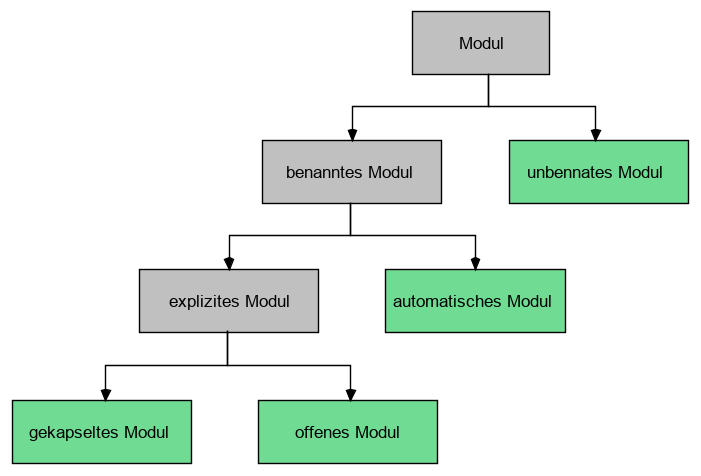
\includegraphics[width=0.7\textwidth]{material/images/module-tree.png}
      \caption{Modularten}
      \label{fig:kopplung}
    \end{figure}

    Die nachfolgenden Modultypen sind Pseudo-Module, die für die Unterstützung der Abwärtskompatibilität eingeführt worden sind. 
    Dementsprechend sollen diese Module eine Brücke zwischen existierender Applikation und der modularisierten Architektur bilden.

    Das \textit{unbenannte Modul} beschreibt alle Klassen und JAR's, die sich parallel zu der Codebasis des Modulpfades auf dem Klassenpfad befinden. Das \textit{unbenannte Modul} beschreibt somit die Legacy-Teil der Codebasis, die noch Migriert werden muss und es noch nicht tun kann. Daher wird mit der Bezeichnung \textit{unbenanntes Modul} eine Zugriffsbarriere zwischen der modularisierten und der legacy Architektur errichtet, die die \textit{expliziten Module} vom Zugriff auf den veralteten Klassenpfad abgrenzt. Denn dieses trägt keinen Namen und kann somit vom Entwickler nicht Pragmatisch referenziert werden.

    In folge dessen entstehen eine asymmetrische Kommunikation zwischen den Architekturen. Die \textit{expliziten Module} arbeiten nur auf dem Modulpfad im neuen System und das \textit{unbenannte Module} darf zusätzlich zu den klassischen Klassenpfad auf den modernen Modulpfad zugreifen. Diese Umsetzung lässt eine inkrementelle Migration der Codebasis auf das Modulsystem zu und bleibt Lauffähig, obwohl die Applikation eine interne Versionsdiskrepanz beinhaltet.

    \begin{figure}[h]
      \centering
      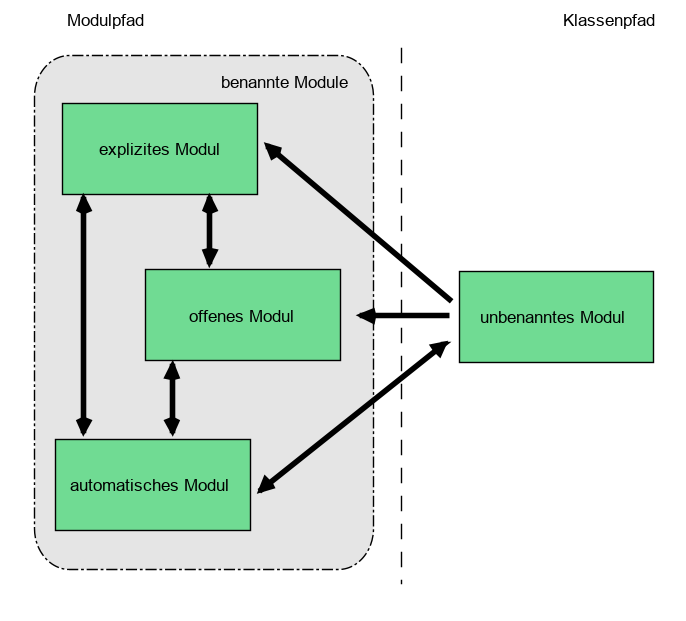
\includegraphics[width=0.7\textwidth]{material/images/module-access.png}
      \caption{Modulzugriffsrechte}
      \label{fig:kopplung}
    \end{figure}

    Das letzte Modul beschreibt ein Modul mit speziellen Verhalt, das sich zwischen den Architekturen stellt und eine Brücke zwischen den Modulpfad und Klassenpfad errichtet. Das \textit{automatischen Module} beschreiben einen Migrationsansatz der bestehenden Bibliotheken, die vom Klassenpfad auf den Modulpfad verschoben werden und keine \textit{Modulbeschreibung} besitzen. Diese kriegen einen Modulnamen zugewiesen und könne über diesen von den \textit{expliziten Modulen} aufgerufen werden. Somit übernimmt Java die Kopplung der \textit{automatischen Modulen} mit allen \textit{expliziten Modulen}, indem alle internen Pakete für die Nutzung offen gelegt werden und alle Module auf dem Modulpfad für die Verwendung importiert werden. Somit ist eine Legacy-Bibliothek auf den Modulpfad funktionstüchtig und bietet eine ganz besondere Fähigkeit, nämlich die wechselseitige Kommunikation zwischen den Modulpfad sowie den Klassenpfad. Dank dieser Fähigkeit können Bibliotheken migriert werden und beide Architekturen zu gleich unterstützen. Dieses Verhalten fördert die Entwickler ihren Code für den Modulpfad zu entwickeln, da die nötigen Legacy-Bibliothek der Applikation in beiden Architekturen zugleich verfügbar sind. Dennoch schafft das \textit{automatischen Module} zusätzliche Komplexität in die Architektur, indem alle Module mit diesem verbunden werden. Daraus folgt eine starke Kopplung und somit eine unübersichtliche, starke Abhängigkeit zwischen den Modulen.\bigbreak

    Nichtsdestotrotz bieten die automatische und das unbenannten Modul diverse Migrationsszenarien, die flexible Wege für die Modernisierung der Applikation anbieten. 

  \subsection{Modulkopplung}
    Die Einführung des Modulsystems in Java 9 integriert das Konzept der Aufteilung einer monolithischen Softwareumsetzung in übersichtliche mit einander sachlich verbunden Modulen. 
    Diese Idee sollte zuerst von Java selbst umgesetzt werden, um als Beispiel für den aufbauenden Code zu fungieren.
    In der praktischen Umsetzung formuliert Java die Modulbeschreibung mit Hilfe der \textit{module-info.java} Datei, die drei Kopplungstypen enthalten kann: Die durch \textit{requires, exports} und \textit{opens} Deskriptoren beschrieben wird.

    \begin{figure}[h!]
      \centering
      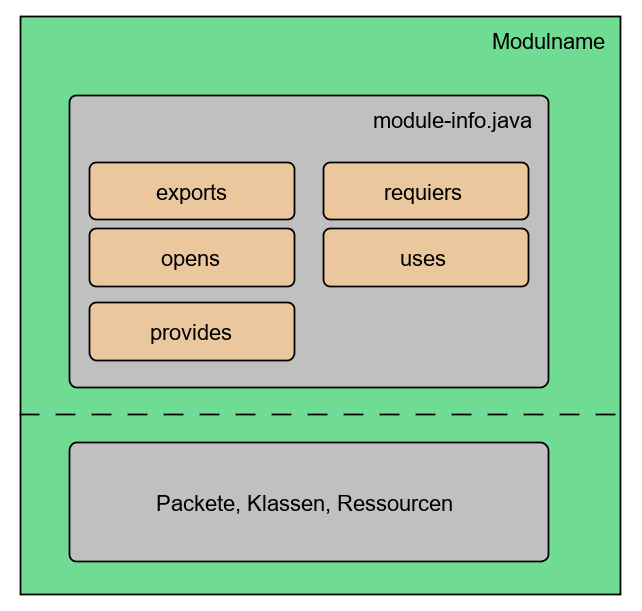
\includegraphics[width=0.5\textwidth]{material/images/module-info.png}
      \caption{Die Schnittstellenbeschreibung \textit{module-info.java}}
      \label{fig:module-info}
    \end{figure}

    Die in der Abbildung \ref{fig:module-info} dargestellten und vorher diskutierten Kopplungsarten, können die Zugriffsberechtigungen ferner einschränken. Diese können ihr Schnittstelle exklusiven Module öffnen, die fortan als eine transitive Verbindung an gebundene Module weiterreichen und obendrein als eine optionale Abhängigkeit deklarieren. Die \textit{uses} und \textit{provides} Schlüssel beschreiben eine Serviceanfrage sowie einen Serviceangebot, die durch den \textit{Java Serviceloader} mit einender verknüpft werden.
    Der \textit{ServiceLoader} übernimmt in diesem Fall die Rolle des Registrierungsdienstes und vermittelt das Angebot und die Nachfrage nach Funktionalität innerhalb der Applikation. Das Konzept der Dienstregistrierung und -verwaltung geht über die Grundlagen hinaus und wird hier nicht weiter diskutiert, dessen ungeachtet ist es eine zusätzliche Möglichkeit die Modulkopplung zu minimieren. \bigbreak
    
    Im Folgenden werden die Möglichkeiten der Kopplungstypen gelistet. Zu beachten ist die Wechselbeziehung zwischen den Modulen, die Pakete anbieten und Module anfordern. 

    \begin{description}
      \item[requires]\hfill
      \newline \textit{requires} Modul
      \newline \textit{requires transitiv} Modul
      \newline \textit{requires static} Modul
      \newline \textit{requires transitiv static} Modul
      \item[exports]\hfill
      \newline \textit{exports} Packet
      \newline \textit{exports} Packet \textit{to} Modul-1, Modul-2
      \item[opens]\hfill
      \newline \textit{opens} Packet
      \newline \textit{opens} Packet \textit{to} Modul-1, Modul-2
      \item [uses]\hfill
      \newline \textit{uses} Service-Schnittstelle 
      \item[provides]\hfill
        \newline \textit{provides} Service-Schnittstelle \textit{with} Service-Impl-1, Service-Impl-2
  \end{description}

  \begin{figure}[h!]
      \centering
      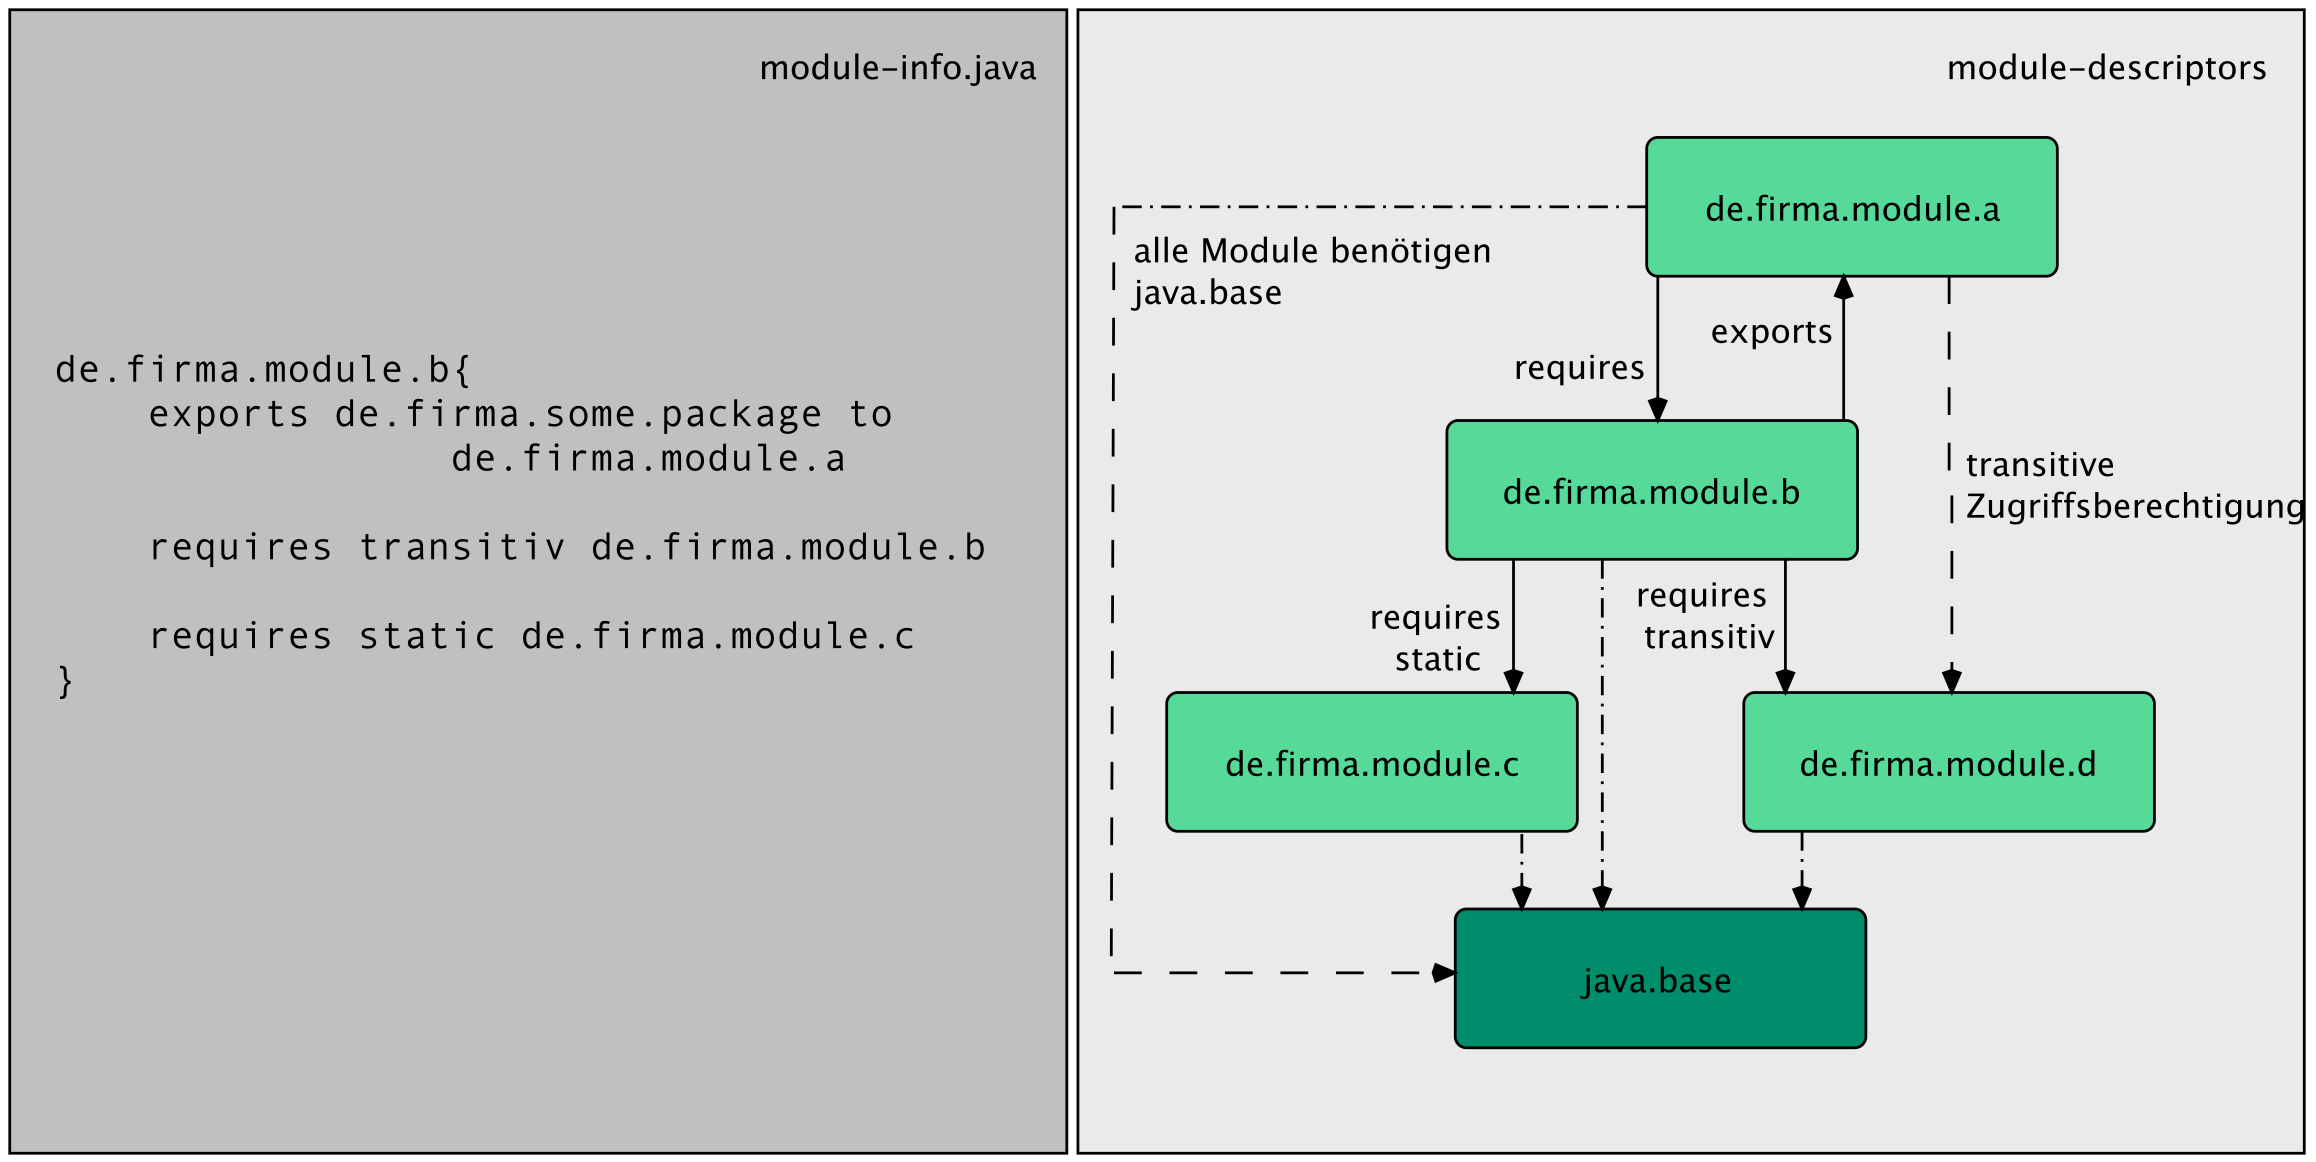
\includegraphics[width=\textwidth]{material/images/transitiv3.png}
      \caption{Abwandlung der Kopplungsarten}
      \label{fig:abw-kopl}
  \end{figure}
\newpage

  Wie in der grafischen Darstellung \ref{fig:abw-kopl} abgebildet, handelt es sich bei den Kopplungstypen um Zugriffsrechte, die als ein offenes Vertrag zwischen Modulen aufgestellt werden. Dementsprechend dienen die Kopplungsschlüssel nicht nur der Lesbarkeit und Autonomie, sondern erweitern die Prozedur des Klassenladens durch explizite Schnittstellen und Zugriffsberechtigungen.

  \subsection{Module-Classloading}
  Im Abschnitt \ref{sec:Namensräume} wurde Namensräume vorgestellt, die Klassen von einender trennen und diese als separate Software Komponenten behandeln, um die Sichtbarkeit der Codebasis gegenüber dem Restsystem abzugrenzen. Jedoch bring dieses Feature einen großen Aufwand mit sich, denn sofern die Applikation über eine große Anzahl an Bibliotheken nutzt und jedes davon auf einem eignen Classloader betreiben möchte wächst der Wartungsaufwand mit der Anzahl der Bibliotheken.

  Mit Hilfe der Module und dessen neuen Ansatz der internen Kapselung, soll dieses Problem adressiert werden, indem separate Zugriffsräume für jedes Modul innerhalb eines Classloaders definiert werden, die sicherstellen, dass die interne Struktur eines Moduls während der Laufzeit nicht kompromittiert werden kann.

  Um die Modulkapselung zu garantieren, wird das im Abschnitt \ref{sec:cls} vorgestellte \textit{Java Classloader System} nicht ersetzt, sondern mit zusätzlichen Kontrollen versehen, die strikt nach deklarierten Modulbeschreibung Zugriff gewährleistet. 
  Im falle der Nichteinhaltung der Zugriffsrechte zwischen den Modulen wirft der Classloader neue Fehlermeldungen wie die \textit{IllegalAccessException} oder die \textit{IllegalAccessError}. Somit bleibt die ehemalige Classloader Hierarchie erhalten, die an das Modulsystem von Java angepasst worden ist.\bigbreak

  Da der JDK nicht mehr aus einer \textit{rt.jar} besteht, sondern dessen Funktionalität auf Module aufgeteilt ist \ref{fig:jdk}, beschäftigt sich das aktualisierte \textit{Classloader System} mit dem laden bestimmter Module, die in Gültigkeitsbereiche eingeteilt sind. Diese müssen nicht mehr das überholte Delegierungsmodell \ref{fig:deligation} von Oben nach Unten durchsuchen, sondern suchen, die für den zuständigen Classloader, bekannten Module zuerst ab, bevor sie die Anfrage an den übergeordneten Classloader delegieren. 
  Die Abbildung \ref{fig:mcl} visualisiert das Laden der Modul-Klassen, die in diesem Fall nicht mehr das unnötige Nachschlagen nach Klassen über die ganze Classloader Hierarchie bearbeitet.

    \begin{figure}[h!]
      \centering{}
      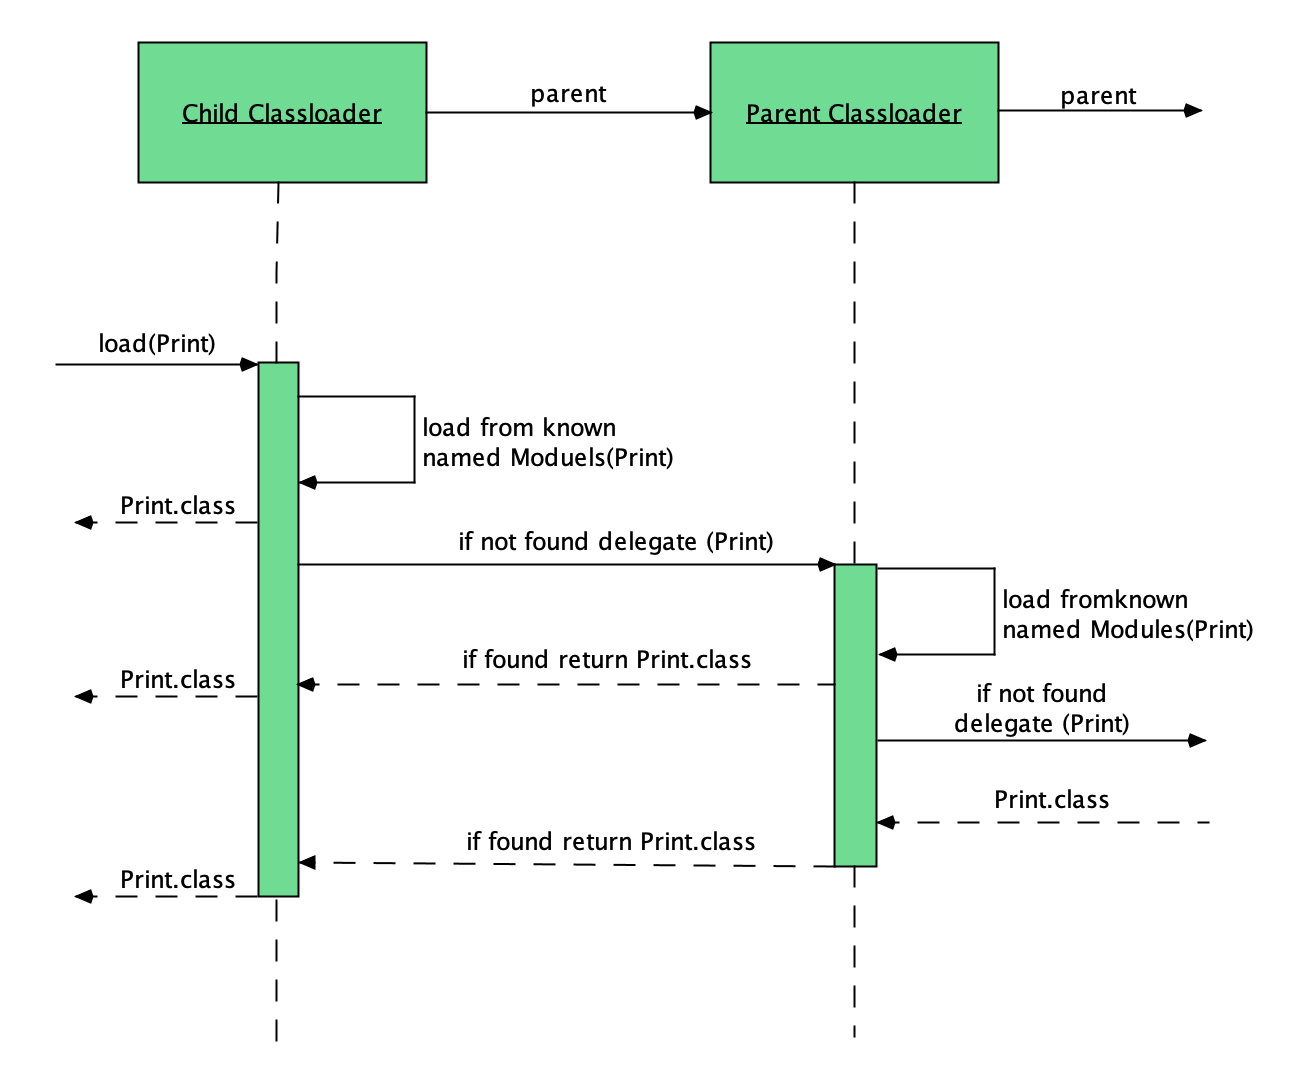
\includegraphics[width=\textwidth]{material/images/module-classloading.png}
      \caption{Modul Classloading}
      \label{fig:mcl}
  \end{figure}

  Indem das Delegierungsmodell abgelöst wurde, werden andere Sicherheitsmaßnahmen für das Schützen der Kern Bibliotheken benötigt. Dies übernimmt jetzt das Modulsystem von Java, indem ein globaler Verbot nach gleichnamiger Benennung von Paketstrukturen gilt. Somit verbietet Java zwei gleiche Bibliotheken auf dem selben Modulpfad und garantiert einen eindeutigen Abhängigkeitsgraphen. \bigbreak

  Um die Klassen aus den Modulpfad zu laden, wird das \textit{Classloader Systems} an den Modulpfad angepasst und lädt jetzt Module, die in Zugriffsgruppen eingeteilt sind. Der \textit{Bootstrap Classloader} besitzt und geniest alle Sicherheitsprivilegien und steht demnach ganz oben in der Classloader Hierarchie. Dieser lädt die \textit{Core Java-SE} und \textit{JDK-Module}, wie \textit{java.base} und \textit{java.logging}. Der Extension Classloader wurde von dem Plattform Classloader ersetzt und lädt jetzt die \textit{Plattform Java-SE} Module, wie zum Beispiel die \textit{java.sql}, oder die \textit{java.xml.ws} Bibliotheken. Und zuletzt bleibt der Applikation Classloader, der unsere Applikationsmodule auf dem Modulpfad verwaltet. 

    \begin{figure}[h!]
      \centering{}
      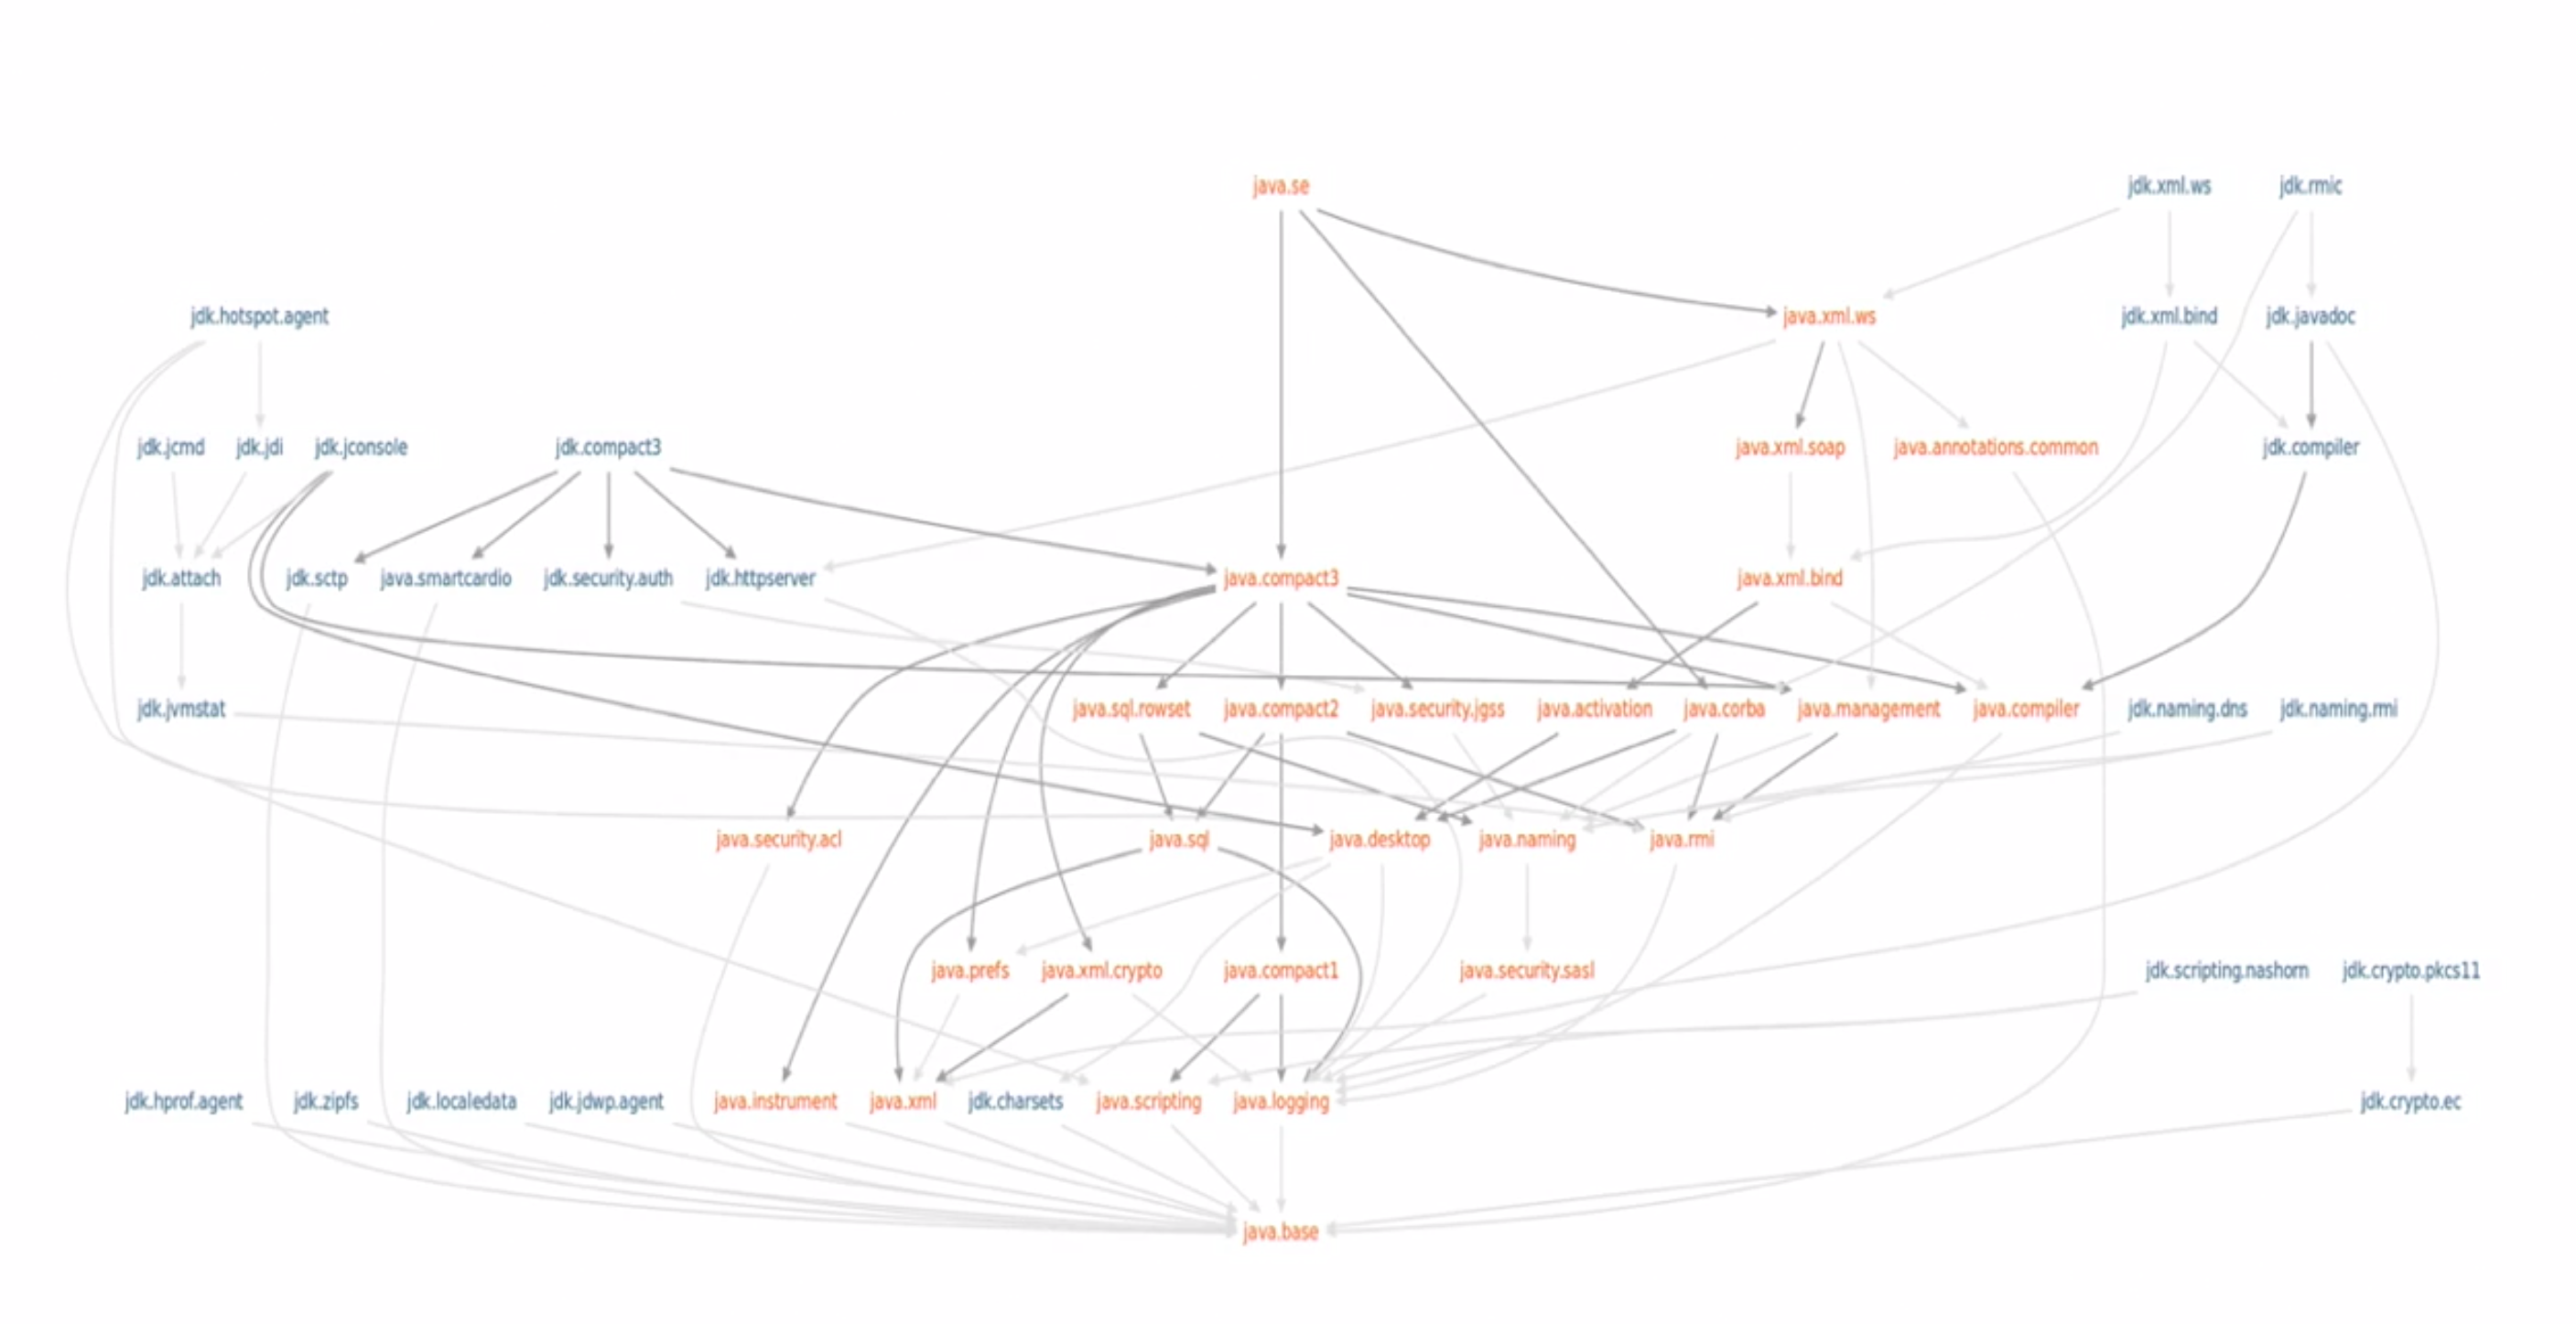
\includegraphics[width=\textwidth]{material/images/jdk.png}
      \caption{Modularisierte rt.jar Bibliotheken}
      \label{fig:jdk}
  \end{figure}

  Obwohl das Modulsystem viele Neuerungen und Aufwertungen der Java Plattform mit sich brachte, sind nicht alle wünsche erfüllt worden, wie zum Beispiel das Nutzen gleichnamiger Bibliotheken mit unterschiedlicher Versionsnummer auf dem selben Modulpfad.
 


\chapter{Migration}

	In dem vorherigen Kapitel wurden Module und ihre Eingenschaften, Konstruktionsregeln sowie Modularten behandelt. Dieses Kapitel beschäftigt sich mit der Fragestellung, wie Altsysteme, die vor dem Modulsystem von Java entwickelt wurden, in dem Modulkontext betrieben werden können und was getan werden muss, um diese den modernen Anforderungen anzupassen und zu modularisieren.\bigbreak

	Die Migration behandelt Systeme, die nicht beständig auf dem aktuellen Stand der Technik gehalten werden, können und an ihren Ausführungskontext gebunden sind. Diese rutschten langsam in den Bereich der Altsysteme, bis ihr Lebenszyklus zu Ende geht und der Legacy-Zustand erreicht ist. Um die Systeme weiterhin zu nutzen, müssen sie in eine Umgebung mit den geforderten Eigenschaften, ohne Änderungen der internen Struktur vorzunehmen, übertragen werden. Dieses Verfahren wird oft im Bereich der Softwaretechnik mit Software Reengineering und Software Neuimplementation verwechselt, dessen Ziel in der Optimierung der Codebasis liegt und nichts mit dem Ausführungskontext zu tun hat. \cite{martens2016ablosung} \bigbreak

	% Migrationsmethoden und der von ihnen gelösten Problemen. 
	Während des Betriebs einer lang gepflegten Kernapplikation, wird der Lebenszyklus öfter überschritten und muss den Migrationszyklus mehrmals durchlaufen. Zum Beispiele kann eine Applikation an Größe gewinnen und muss in die Cloud ausgelagert werden, die Anforderungen können sich verschieben und der Technologie-Stack muss an die Marktbedürfnisse angepasst werden, darüber hinaus kann der Ausführungskontext einen großen Versionssprung hinter sich lassen, der das Warten der Software unter den momentanen Bedingungen unmöglich macht. \newline
	Dem zufolge ist das Umfeld der Software Entwicklung eine dynamische Umgebung, denn auch mit einer gut durchdachte Architektur kann nicht garantiert werden, dass in der Zukunft heutige Paradigmen, Werkzeuge und Aufgabenbereiche denselben Kurs behalten. Deswegen existieren bereits sämtliche Migrationsstrategien, die als ein Leitpfaden den Entwickler durch die Migration führen. \bigbreak

	Im folgenden Kapitel werden Ansätze vorgestellt, die Monolithische- sowie Bibliotheksanwendungen in das modulare System überführen ohne Änderung an der interne Funktionalität durchzuführen. 


\section{Legacy-System}

	Der Begriff \textit{Legacy-System} beschreibt ein altes System, das innerhalb einer Organisation länger als der geplante Lebenszyklus in Betrieb bleibt. Der englische Begriff \textit{Legacy}, zu deutsch Erbe, bezieht sich nicht auf das Alter der Software, sondern auf die Interpretation der Software als Erbe. Da die Umsetzung von früheren Entwickler Teams durchgeführt wurde, die sich an damaligen Konzepten und Strategien bedienten, ergab die Lösung ein Erbe mit bestimmten Einschränkungen, die für die zukünftige Erweiterung der Software eine große Rolle spielen. Denn, die typischerweise veralteten Verfahren und Technologie lange Lebenszyklen mit umfangreichen Veränderungen und Erweiterungen erfahren haben \cite{sneed2016softwaremigration}. \bigbreak

	Zu meist handelt es sich um sogenannte Kernsysteme, zur Unterstützung wesentlicher Geschäftsprozesse eines Unternehmens. Sie sind in der Regel geschäftskritisch und können nicht ohne großen Aufwand und Risiko für das Unternehmen ausgetauscht werden. Aufgrund ihres langen Lebenszyklus, ihrer Komplexität und ständigen Überarbeitungen ist die Logik solcher Systeme oft unübersichtlich und schlecht dokumentiert. Ihre Implementierung kann zusätzlich früher geltenden Standards unterliegen und anderen Programmierparadigmen folgen, die nur schwer verständlich sind. Daher sind Geschäftsprozesse und Geschäftsregeln im Code versteckt und müssten z.\,B. für eine Neuimplementation erst rekonstruiert werden \cite{martens2016ablosung}.

\section{Migration} \label{ssub:migration}

	% schau in diesem buch nach einer defenition  mit den storchen 
	Die Softwaremigration bezeichnet die Überführung eines Softwaresystems in eine andere Zielumgebung oder in eine sonstige andere Form, wobei die fachliche Funktionalität unverändert bleibt. Als Ausgangspunkt steht dabei immer ein bestehendes System, das an Anforderungen und Techniken des Anwendungsbereiches angepasst werden muss \cite{sneed2016softwaremigration}. Die Adaption an den neuen Anwendungsbereich geschieht zu meist nicht problemlos und muss System- und Kontextbezogene Hürden überwinden. 

\section{Migrationshürden} \label{MigH}

	% Einleitung: hier kommen allgemeinen Beispiele der Migrationsproblematik 
	Die Migrationshürden sind fest mit dem Anwendungskontext verbunden und hängen stark von der Beschaffenheit der neuen Umgebung ab. Da in unserem Fall die Migration innerhalb der Java Umgebung stattfindend, müssen die Neuerungen des Modulsystem analysiert und auf den bestehenden Zustand der Applikation abgebildet werden.\bigbreak

\begin{itemize}
	% Hauptteil: Probleme und Hürden, die der neue Kontext macht
	\item Die Probleme bei dem Modulsystem beginnen mit den Zugriffsrechten auf die Core-JDK API's. Diese sind ab sofort in dem Modul gekapselt und bieten eingeschränkte Möglichkeit sie aufzurufen. Nichtsdestotrotz stellt Java für viele der gekapselten API's einen Ersatz zur Verfügung, wodurch zahlreiche Probleme mit einem relativ geringen Aufwand behoben werden können. \cite{masteringJava9,modulProgJava9,modulMitJava9,javaMod9} 


	\item Im Weiteren verbietet das neue Modulsystem namensgleiche Pakete in verschiedenen Modulen. Dieses adressiert das vorher besprochene Problem aus dem Kapitel \ref{sec:nam}, nämlich den Zugriff auf privat deklarierte Pakete aus fremden Modulen. Trotz dem gibt es Bibliotheken mit ähnlicher Paketstruktur die nicht böswillig sich Zugriff verschaffen wollen, sondern spiegeln eine Standardstruktur einer Bibliothek wieder, wie zum Beispiel \textit{de.firma.input.reader} kann in mehreren Bibliotheken eines Unternehmens existieren und wird ab Java 9 nicht mehr zulässig sein. Somit müssen Module mit ähnlicher Struktur angepasst werden um den nächsten Modularisierungsschritt durchführen zu können. \cite{masteringJava9,modulProgJava9,modulMitJava9,javaMod9} 


	\item Der Classloader-Typ des Applikation-Classloaders wurden überarbeitet und infolgedessen auch das Arbeiten mit den ehemaligen URLClassloader Methoden. Der bestehende Code, der den URLClassloader exzessiv nutzt und zum Beispiel Ressourcen aus verschiedenen Quellen lädt, muss auf den \textit{SecureClassLoader} oder  \textit{ClassLoader} aufgewertet werden, um funktionstüchtig zu bleiben. \cite{oracModClassLoader} 


	\item Einer der Kritischen Veränderungen, die die Modultatform mit sich bringt, ist der Verbot von zyklischen Abhängigkeiten von Modulen untereinander. Diese dürfen sich nicht gegenseitig mit den Schlüssel \textit{require} koppeln, da sonst eine Veränderung in einem Module zwangsläufig eine Änderung in den anderen Modulen hervorrufen kann. Dieser Still kann sich schnell über die ganze Applikation verbreiten und kleine Änderungen an einer Stelle zu unübersichtlichen Seiteneffekten führen. Genau diese Probleme adressiert das Modulsystem in erster Linie und verbiete aus diesem Grund Zyklen in den Applikationsentwurf. Um bestehende Zyklen in einer Applikation zu lösen, muss die Funktionalität genau betrachtet und in kleine unabhängige Aufgaben aufgeteilt werden. Somit werden Zyklen aufgebrochen und die Aufgabestellung jedes Moduls klar definiert. \cite{java9modRevealed,modulProgJava9,modulMitJava9} 
\end{itemize}

\section{Migrationsarten} \label{Migratiosarten}

	% Schluss: Bewegen uns auf die möglichen Migrationsstrategien für die Modularisierung.
	Da jede Applikation spezifisch Migrationsanforderungen besitzt, gibt es unterschiedliche Verfahren, die sich bestimmten Kriterien widmen. Dementsprechend sollte man die gegebene Applikationsbeschaffenheit ermitteln und dessen Probleme auf die passende Migrationsstrategie abbilden. Die prominenten Migrationsstrategien der Software Techniken sind \textit{Chicken Little} und \textit{Butterfly}, die zwei der gängigsten Arten der Softwaresystem Migration beschreiben. \cite{sneed2016softwaremigration} \bigbreak


	% Chicken Little
	Softwaresysteme, die nach dem \textit{Chicken-Little-Ansatz} migriert werden, zerlegen das System in mehrere Migrationspakete, die einzeln in kleinen inkrementellen Schritten in die neue Zielumgebung überführt werden. Damit der Betrieb des Systems nicht für die Zeitdauer der Migration ausfällt, existieren alte, neue und migrierte Teilsysteme nebeneinander. Die korrekte Kommunikation der Softwarebausteine muss über entsprechende Kommunikationskanäle errichtet werden und gestaltetet damit einen Brücke zwischen Alt- und Neuentwicklung, die zusammen einen gemeinsame Ressourcenbasis nutzen können. \cite{sneed2016softwaremigration} \bigbreak

	% Butterfly 
	Der \textit{Butterfly-Ansatz} geht von einer separaten Entwicklung der Applikation in der neuen Umgebung aus. Dies hat zu folge, dass die Altapplikation in Betrieb bleibt und unverändert ihre Aufgabe erfüllt, bis der Nachfolger, der parallel zu dem Betrieb entwickelt und getestet wird, die Funktion korrekt widerspiegeln kann. Im Anschluss werden Ressourcenbestände in kleinen Paketen an die Applikation im neuen Kontext transferiert und das Altsystem abgeschaltet. Das Butterfly-Verfahren vermeidet also während der Migration den simultanen Zugriff auf Legacy- und Zielsystem. \cite{sneed2016softwaremigration} \bigbreak

	% Ein text der auf die nächsten Kalitel einführt 
	Zwischen den beiden vorgestellten \textit{Migrationsideen} hat sich das Java Team für die Unterstützung der Schrittweise-Migration entscheiden, die eine Applikation in kleine Softwareeinheiten aufteilt und langsam auf den neuen Modulpfad migriert. Der parallele Betrieb der neuen sowie alten Struktur wird durch eine interne Brücke, die korrekte Kommunikation zwischen den Klassenpfad und den Modulpfad errichtet umgesetzt. Die Implementation der Kommunikationsbrücke und ihrer Charakteristika, die eine kritische und verantwortungsvolle Aufgabe in der Migrationsprozess trägt, wird für uns von dem Java Team zur Verfügung gestellt. Somit unterstützt und führt das Modulsystem von Java den Entwickler bei der Hand zu der korrekten, sicheren, modernen und funktionstüchtigen Modularchitektur. \newline
	Ungeachtet dessen, ist die Migration einer Applikation zu diesem Zeitpunkt nicht zwingend und kann innerhalb des Modulsystems weiterhin betrieben werden, da diese keine spezielle Hilfsmittel von der Umgebung fordern.\bigbreak

	In den nachfolgenden Kapiteln werden unterschiedliche Varianten der Migration und des Betriebs einer Applikation innerhalb des Modulsystems vorgestellt. 


\subsection{Plattform Migration}
	Die simpelste Migration ist eine reine Plattform Migration ohne Änderungen an der Software vorzunehmen, wie in der Abbildung \ref{fig:PM} dargestellt. Dies ist möglich, dank der Unterstützung des Klassenpfades, der in diesem Fall unsere Applikation als ein \textit{unbenanntes Modul} im Modulsystem betreibt. Wie bereits im Kapitel \ref{Modularten} angesprochen, bietet dieses Modul den Betrieb der Legacy Anwendung in der neuen Umgebung mit dem geringen Anteil der möglichen Vorteilen, wie zum Beispiel den Sicherheitsupdates. Zusätzlich behält die Applikation ihre monolithische Architektur und vermisst alle Modulsystem Features, die im Kapitel \ref{sec:ZdM} und \ref{sec:ME} angesprochen wurden.

	\begin{figure}[h]
		\centering
	    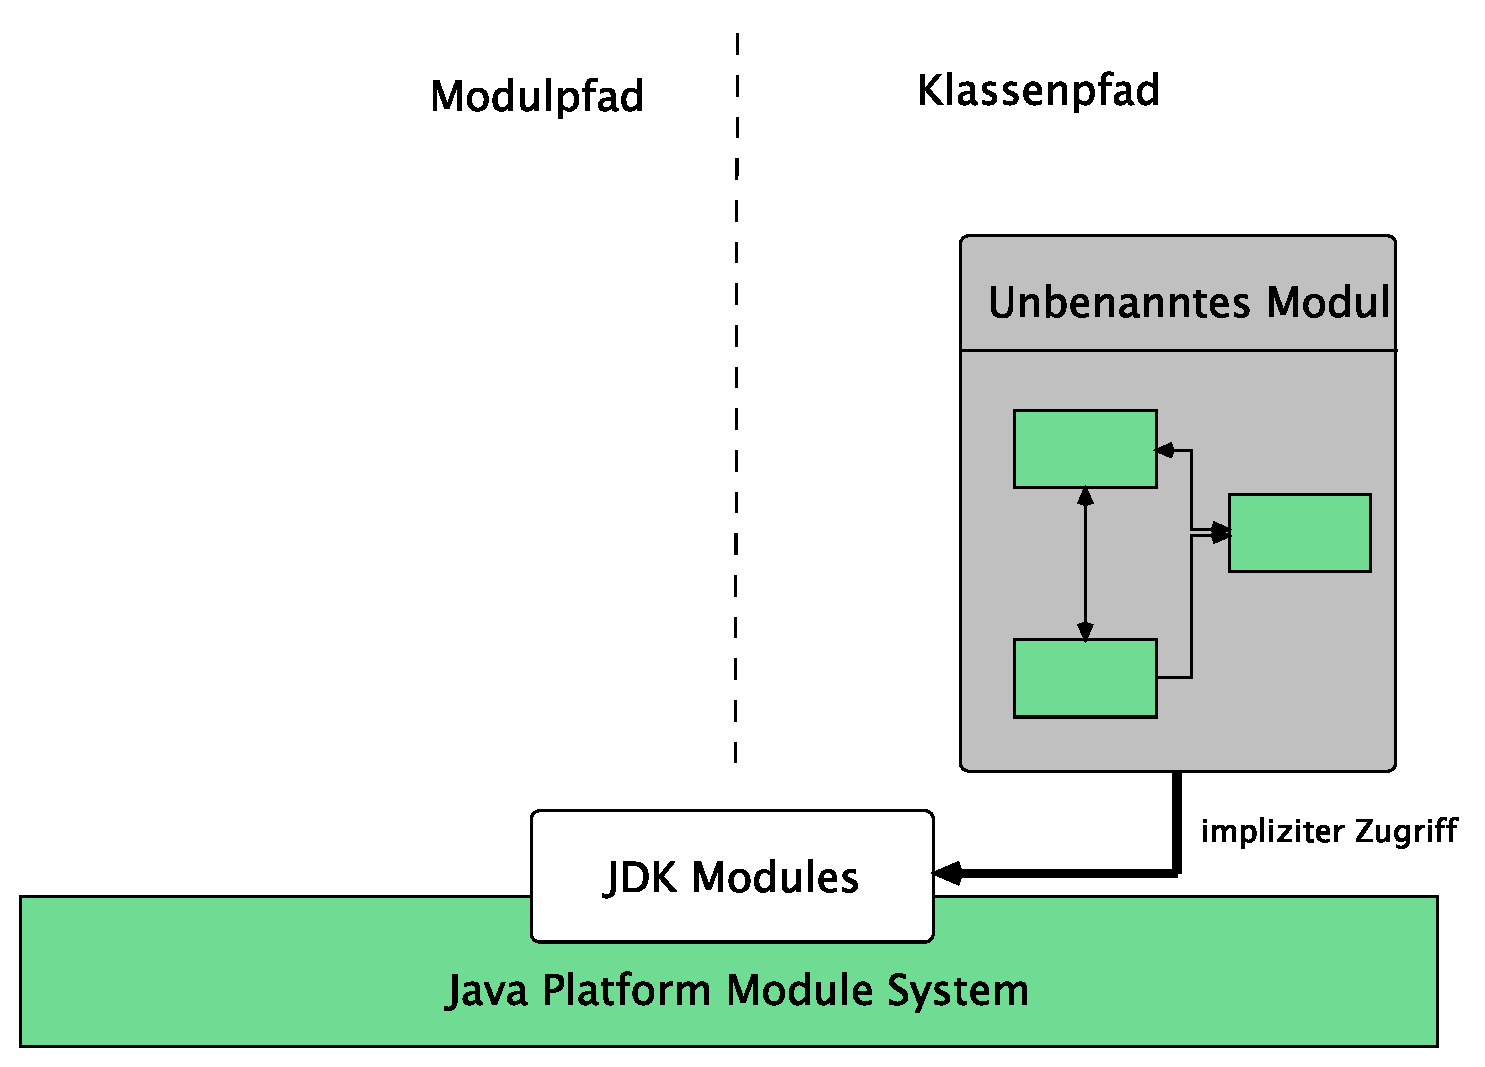
\includegraphics[width=0.8\textwidth]{material/images/platform-migrate.pdf}
	    \caption{Plattform Migration \cite{modulMitJava9}}
	    \label{fig:PM}
  	\end{figure}

	Eine weitere Möglichkeit wäre es die Applikation und ihre Bibliotheken auf den Modulpfad zu migrieren und als \textit{automatische Module} zu betreiben. Somit wäre der alte Klassenpfad  nicht mehr im Applikationsdesign vorgesehen und fokussiert die Entwickler auf die Arbeit mit dem Modulpfad. Dennoch lässt sich nicht jede Anwendung in diesem Still migrieren, denn die Hürden aus den Kapitel \ref{MigH}, wie die \textit{Zyklen-Freiheit} sowie der verbot der \textit{Split-Packages} in Legacy Bibliotheken nicht immer gegeben ist. 



\subsection{Top Down Migration}
	Die \textit{Top-Down} Migration behandelt die Migration von Oben nach Unten, dabei werden zuerst die Applikation und im Nachhinein die Drittanbieter Bibliotheken migriert. Dafür müssen die Applikationspakete auf Abhängigkeiten geprüft und entsprechende Module sowie Modulbeschreibungen nach den im Kapitel \ref{sec:MEK} besprochenen Kriterien erstellt werden. Mit dieser Methode werden die Drittanbieter Bibliotheken zuletzt betrachtet, da es bei diesen um Fremdcode handelt. \newline
	Da nach der Prüfung der Abhängigkeiten ein Graph entsteht, verweist dieser ab einen gewissen Punkt die Bibliotheksabhängigkeit der Applikation, die wiederum von weiteren Bibliotheken abhängen. Somit können die Wurzel der benötigten Drittanbieter Bibliotheken einer Applikation ausfindig gemacht und als \textit{automatische Module} in den Modulpfad eingebunden werden. Somit können diese, wie bereits in im Kapitel \ref{Modularten} behandelt, sowohl mit der Applikation als auch mit den Legacy Elementen ihrer eigener Abhängigkeiten zugleich interagieren. Zum Schluss kümmert man sich um die Bibliotheken auf dem Klassenpfad, indem diese ersetzt oder selbständig weiterentwickelt werden, mit dem Ziel die Gesamtapplikation auf dem Modulpfad zu übertragen. \cite{javaMod9,modulProgJava9,java9modRevealed,modulMitJava9,masteringJava9}\bigbreak
	\begin{figure}[h]
		\centering
	    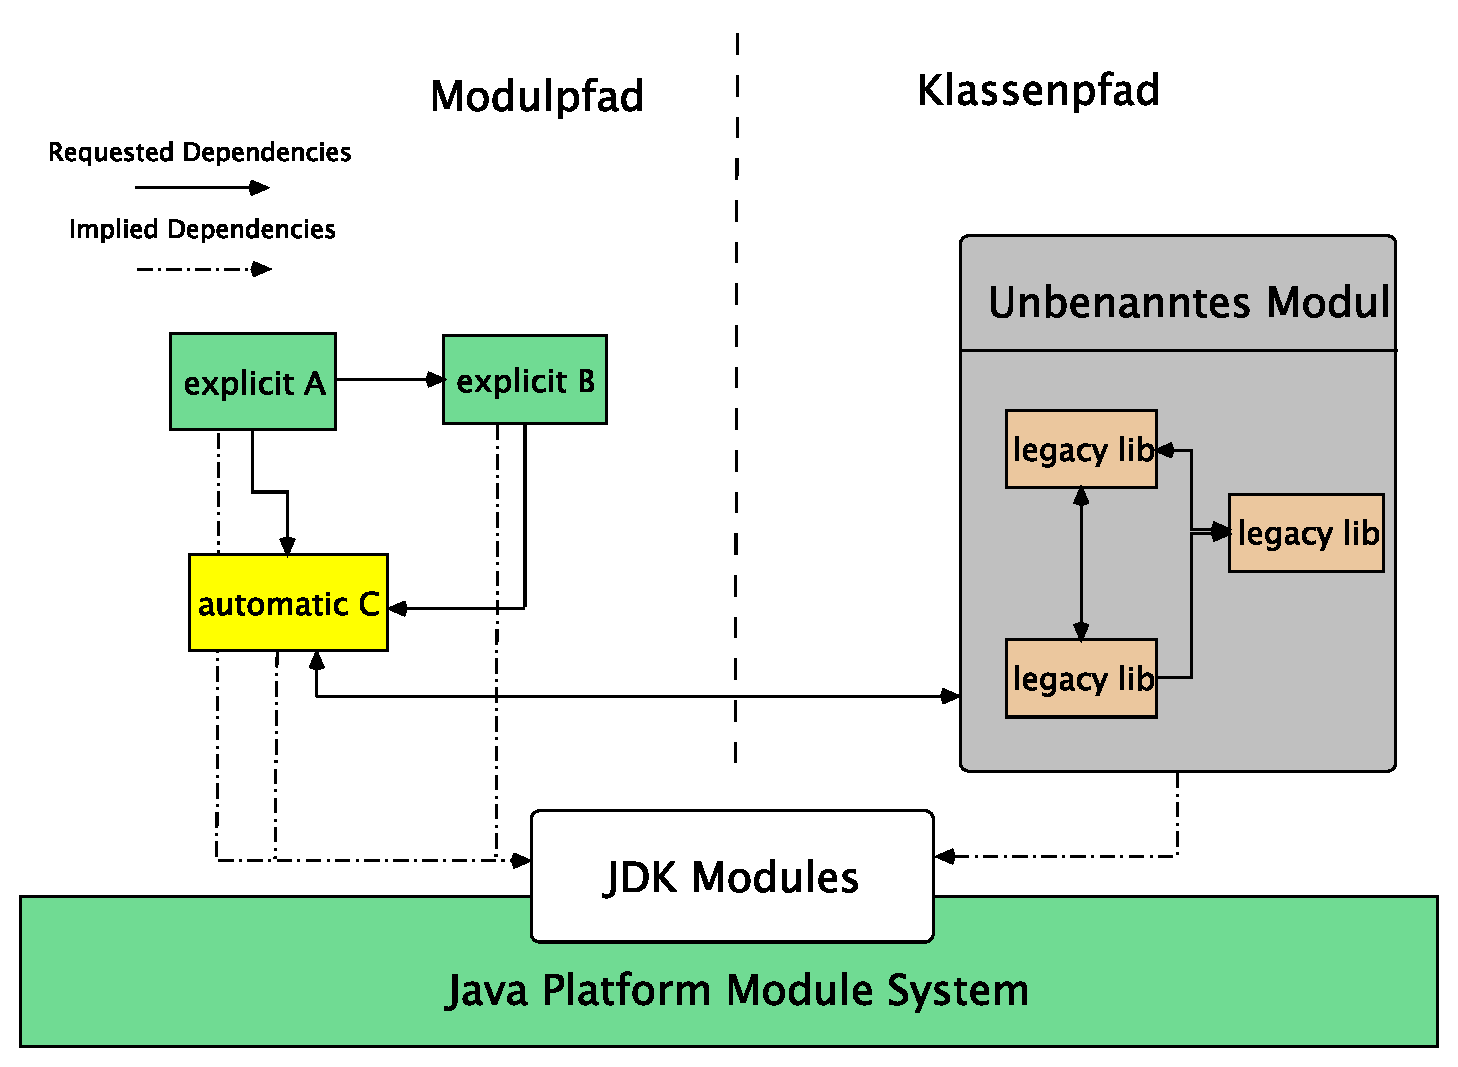
\includegraphics[width=0.8\textwidth]{material/images/top-down-migrate.pdf}
	    \caption{\textit{Top Down} Migration}
	    \label{fig:TDM}
  	\end{figure}

	Diese Migration ist besonders vorteilhaft bei Applikationen, die eine geringe Codebasis besitzen und in einem kurzen Zeitraum eine modularisierte Form annehmen können. 

\subsection{Bottom Up Migration} \label{sec:bottomUP}
	Die \textit{Bottom Up} Migration behandelt lose Module zuerst, denn diese haben keine Abhängigkeiten und bieten eine gekapselte Funktionalität an. Um herauszufinden welche Module sich für den initialen Migrationsschritt eignen, kann der Abhängigkeitsgraph mit Hilfe des \textit{JDepth} erstellt werden. Module die als Blätter aufzufinden sind, können zuerst migriert werden, da sie keine Kinderknoten und somit keine Abhängigkeiten besitzen. Im weiteren Verlauf der Migration werden die übrig gebliebenen und neu entstandenen Blätter des Abhängigkeitsbaums abgearbeitet, bis die ganze Applikation, samt der Drittanbieter Bibliotheken, sich auf dem Modulpfad befindet. Während der Migration müssen natürlich die im Kapitel \ref{sec:MEK} besprochenen Kriterien erfüllt werden, um eine robuste Umsetzung zu erreichen. \cite{javaMod9,modulProgJava9,java9modRevealed,modulMitJava9,masteringJava9} \bigbreak
	\begin{figure}[h]
		\centering
	    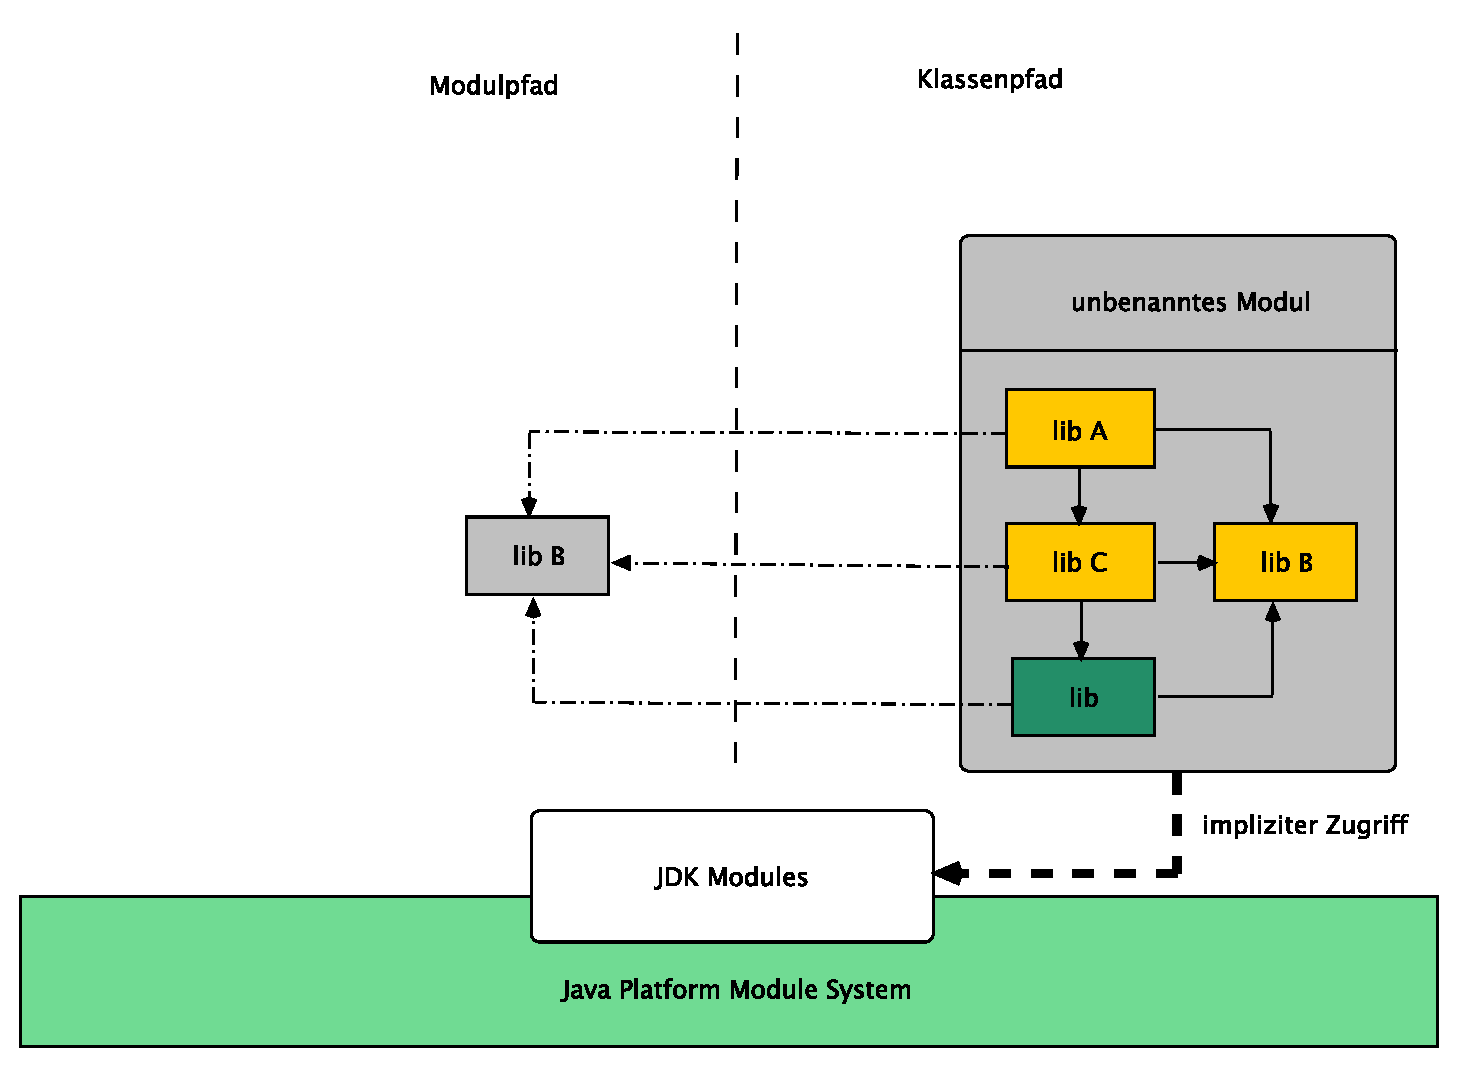
\includegraphics[width=0.8\textwidth]{material/images/bottomUP.pdf}
	    \caption{\textit{Bottom Up} Migration \cite{modulMitJava9}}
	    \label{fig:BUM}
  	\end{figure}
	In der Abbildung \ref{fig:BUM} wird der erste Schritt der \textit{Bottom Up} Migration angedeutet, indem die \textit{lib B} als erste auf den Modulpfad migriert wird. Diese hat keine Abhängigkeiten und ist der perfekte Kandidat für den initialen Schritt. Als Nächstes bietet sich die \textit{lib} Bibliothek für die Migration an, da sie keine weiteren Abhängigkeiten in den Klassenpfad besitzt. Jedoch ist es eine Drittanbieter Bibliothek und kann von uns nicht bearbeitet werden. Aufgrund dessen wird die \textit{lib C} für  den nächsten Migrationsschritt ausgewählt und als ein \textit{automatisches Modul} auf den Modulpfad migriert. Somit kann dieses die \textit{lib} und \textit{lib B} zugleich nutzen. Als Nächstes ist die \textit{lib A} an der Reihe, dessen komplette Abhängigkeiten sich bereits auf dem Modulpfad Befinden. In der Konsequenz befinden sich alle Applikationsbibliotheken auf dem Modulpfad. \cite{javaMod9,modulProgJava9,java9modRevealed,modulMitJava9,masteringJava9} \bigbreak

	Die \textit{Bottom Up} Migration bietet sich bei bereits aufgeteilten Applikationsarchitektur an, die über eine Menge von \textit{Jar} Bibliotheken betrieben wird. Diese braucht weniger Aufwand, um den Monolithen zu zerlegen und sind bereits über Schnittstellen mit einander Verbunden. \cite{modulProgJava9,modulMitJava9}









\chapter{Analyse der Ausgangssituation}\label{cha:ausgangssituation}
	Dieses Kapitel diskutiert die Motivation für die Abschlussarbeit, setzt klare Ziele sowie Rahmenbedingungen und erörtert den Einfluss des Java Modulsystems auf Renew wie auch die derzeitige Plugin-Architektur. Des Weiteren wird ein Zustand ermittelt, der als Basis für die nachfolgenden Prototypen gelten wird.

\section{Anforderungsanalyse} 
	Indem der Java-JDK mit der neunten Version von Java modularisiert wurde, ändern sich grundsätzlichen Funktionsrichtlinien der Plattform, die Konsequenzen für bestehende Systeme mit sich bringen. Denn das Modulsystem von Java führt eine obligatorische Kapselung der Code-Komponenten ein, die über erweiterte Sicherheitsmechanismen verfügen und nur über explizite Schnittstellen geladen und angesprochen werden können.\newline 
	Diese Abschlussarbeit beschäftigt sich mit der Untersuchung von Anforderungen der modularisierten Java Plattform, sowie mit dem entsprechenden Aufwand für das Anpassen bestehender Systeme. \newline
	Für die Umsetzung muss ein grundlegendes Migrationsverfahren erarbeitet und angewandt werden, welches eine Migration auf das Modulsystem von Java ermöglicht. Da die Migration bestehender Systeme nicht in einem Schritt durchgeführt werden kann, müssen Charakteristika für Module formuliert werden, um bestehende Systemelemente innerhalb einer ausgereiften Software mit den entsprechenden Eigenschaften zu erweitern.\newline
	Jede kleine Änderung in einem komplexen System bringt große Risiken mit sich, die das sauberen Arbeit der Software in Frage gestellt. Daher ist der Übergang auf das Modulsystem von Java mit Unsicherheit verbunden, zumal dieses Zeit kostet, im Code verankertes Geschäftswissen umstrukturiert und keine sichtbare Softwareerweiterung für den Endkunden darstellt. Demnach liegen die Schwerpunkte der Migration in der Konsistenz der gegebenen Software im neuem Kontext, den Mehrwert sowie in dem Aufwand der Umsetzung. \bigbreak

	Um die gegebenen Anforderungen an eine Applikation zu stellen bedarf es eine passende Projektstruktur und Umsetzungswerkzeuge, die eine Modulmenge kompilieren und verpacken. Zu diesen Zweck soll das Java basierte Gradle Werkzeug eingeführt werden, das eine kompakte und mächtige Ausdrucksform für das Erstellern von Softwaresystemen Entwicklungsumgebung unabhängig anbietet. \bigbreak

	Für die Umsetzung der erarbeiteten Konzepte steht der Renew Simulator und das Mulan Rahmenwerk zur Verfügung, die in dieser Abschlussarbeit Migrationsszenarien erleben.\newline 
	Das erste Szenario soll eine kontinuierliche Migration einer Software auf das Modulsystem modellieren. Im Gegensatz dazu, wird im zweiten Szenario alt Software auf eine modularisierte Code-Basis aufgesetzt und der parallele Betrieb begutachtet.  

\section{Anforderungsspezifikation} 
	Für den Anwendungskontext der Modularisierung einer größeren Anwendung steht Renew und Mulan zur Verfügung, jedoch übersteigern eine vollwertige Modularisierung von Renew und Mulan den Zeitrahmen dieser Abschlussarbeit, da die Umstellung jedes einzelne Plugins auf organisierte Modulverbände eine zeitintensive Aufgabe verkörpert. Jedes einzelne Plugin muss analysiert, reorganisiert, auf Module zerlegt und bestens mit einander Verzahnt werden. Darüber hinaus müssen die entstandenen Module mit allen gegenwärtigen Plugins abgestimmt werden, da das Plugin Modulverband generell andere Schnittstellen anbieten wird. \bigbreak
	Dementsprechend wird die Modularisierung auf einzelne Plugins reduziert, die für die Darstellung der UI sowie die grundsätzliche darunterliegende Logik zuständig sind. Um die Kommunikation im bestehenden System zu garantieren, behalten die entstandenen modularisierten Plugins ihre Schnittstellen. Im Folge dessen wird die Funktionalität aller Plugins nicht beeinträchtigt und garantiert dem Gesamtsystem einen nahtlosen Übergang auf den Modulpfad. Hierfür werden die Plugin Module mit den entsprechenden Konfigurationsdateien erweitert und mit den notwendigen Plugins verzahnt. In der Konsequenz wird die Umsetzung nur die minimalen Anforderungen des Modulsystems realisieren und das Zerlegen der internen Struktur der Plugins aus der Sicht lassen, obwohl es eine wünschenswerter Schritt in Richtung der Modularisierung wäre. \newline 
	Trotz allem müssen die Plugin Projekte von Renew zusätzliche Module unterstützen und die Möglichkeit bieten Renew zu erweitern, um weitere Module innerhalb eines Plugins erstellen zu können. Dafür benötigen alle Plugins eine neue Projektstruktur die das gewünschte Verhalten umsetzt und die empfohlene Modulorganisation unterstützt. Dieses trägt die Maven konforme Projektstruktur, die Java Klassen, Ressourcen und sonstige Artefakte nach einem standardisierten Muster verwaltet.  \bigbreak

	Des Weiteren muss die Konfiguration des Projektes von der Entwicklungsumgebung gelöst werden, um den Entwickler nicht in seinem Arbeitsablauf einzuschränken und die Entwicklungsumgebung seiner Wahl zu nutzen. Dazu soll die existierende Ant Umgebung mit Gradle ersetzt werden. Diese erleichtert das Verwalten sowie Verpacken der Software und verspricht zusätzlich eine kohärente Arbeitsweise mit dem Modulsystem von Java, indem das Verwalten der Modulabhängigkeiten sich in beiden Systemen widerspiegeln. Diese Eigenschaft soll auf die modularisierten Version von Renew angewandt und evaluiert werden. \bigbreak

	Da der Renew Simulator von verschiedenen Abschlussarbeiten beleuchtet und erweitert wird, beinhaltete die Applikation verschiedene Techniken der Softwareentwicklung, wie zum Beispiel das Generieren von Java Klassen mit dem \textit{JavaCC} Compiler. Dementsprechend existieren ältere Verfahren innerhalb von Renew, die sorgfältig auf Kompatibilität mit der neuen Umgebung untersucht und migriert oder ersetzt werden müssen. \bigbreak
	Das Aufbereiten der Grundlagen sowie der Ausgangssituation sind essenzielle Schritte einer Migration, da diese das Fundament für die Planung und Umsetzung legen. Zusätzlich leitet die Ausgangssituation das Migrationsszenario, das eine beispielhafte Schritt für Schritt Migration oder Integration demonstriert und evaluiert.\bigbreak

\section{Motivation}\label{sec:motivation}
	Es gibt mehrere Gründe warum Renew die Migration auf das Modulsystem durchführen sollte. Im Folgenden werden die wesentlichen Gründe, die für die Migration sprechen diskutiert.  

\subsection{Architektur} \label{sub:architektur}
	Die initiale Entwicklung von Renew begann mit einer monolithischen Architektur. Diese erfüllte die nötigen Anforderungen, eignet sich jedoch nicht für Entwickler mit geringer Kenntnis über die Gesamtarchitektur und den darunterliegenden theoretischen Konzepten. Daher wurde eine Plugin-Architektur aufgesetzt, die es ermöglichte Studenten Renew mit Logik innerhalb eines Plugins zu erweitern. Dieses Verfahren trägt bereits den Gedanken der Modularisierung in sich, da die Gesamtarchitektur in Bestandsteile zerlegt und mit einander entkoppelt verknüpft wird. Somit ist die Einführung des Modulsystems der nächste Schritt in Richtung erweiterbare und zusammensetzbare Systeme vorgenommen.

\subsection{Verkürzter Entwicklungszyklus}\label{sub:vez}
	Die Aufteilung einer monolithischen Architektur auf eine Plugin-Architektur war ein großes Ereignis für Renew. Denn mit der Zerlegung der Gesamtarchitektur, wurde die Komplexität auf die entstandenen Komponenten aufgeteilt und erlaubte eine mühelose Weiterentwicklung der Applikation über die Plugins. \bigbreak

	Obwohl die Renew Plugin-Architektur lange im Betrieb blieb, hatte das Plugin-System die Codebasis umorganisiert, ohne diese zu verändern. Diese führt zu altem, unverständlichem Code aus der Java 1.4 (2002) Version, mit dem viele Konzepte und Architektur Entscheidungen getroffen wurden. Nach fast 18 Jahren Betrieb altert die Codebasis sowie die Ideen und Konzepte für die Umsetzung ihrer Funktionalität. Besonders konfus und aufgebläht können Funktionsumsetzungen erscheinen, die heute von Java 12 in ein paar Zeilen gelöst werden können. Der zügige und rapide Wandel der Software Paradigmen und deren optimaler Einsatz in der Software Architektur ist ein Teil des Fortschritts und muss in die Planung des Lebenszyklus der Applikation mit einkalkuliert werden. \newline

	Daher ist die Modularisierung und dessen Anforderung an die Struktur und Inhalt ein wichtiges Ereignis für den Renew Lebenszyklus. Denn dieser erreicht wieder sein Ende und wird mit dem Modularisierungsschritt zurückgesetzt. \bigbreak

	Renew's Entwicklungseinheit ist das Plugin. Diese repräsentiert ein bestimmtes Feature mit einem eigenen Lebenszyklus, wie zum Beispiel ein Formalismus, Simulator oder Fenster Management Plugin. Diese müssen Daten entgegennehmen, diese verarbeiten und wieder ausgeben. Demzufolge bündelt ein Plugin mehrere Fähigkeiten, die zusammen ein Feature verkörpern. Somit können Codeänderungen an mehreren Stellen im Plugin das Verhalten des Plugins beeinträchtigen und müssen auf das Gesamtverhalten des Plugins und seiner Nutzer getestet werden. Mit der Einführung der Module, kann das Plugin in kleinere Einheiten zerlegt werden, die anschließend eine gekapselte Teilfunktionalität des Plugins in sich tragen und Auswirkungen der Modifikation eingrenzen. Diese sind klein, leicht änderbar, ersetzbar und besitzen einen eignen Lebenszyklus. Somit verkürzt sich die Entwicklungsdauer einer Änderung und bietet eine Möglichkeit kooperativ und parallel an einem Plugin zu arbeiten. \newline

	Demnach erweitert die Modularisierung den Renew Kontext und erlaubt das Entwickeln von Plugins in Rahmen eines Studenten Projekts, indem Teilaufgaben eines Plugins auf Module zerlegt und parallel von Studenten bearbeitet werden können. Darüber hinaus ist das Zusammenführen der Ergebnisse eine konfliktfreie Angelegenheit und bedarf keine komplette Gruppenaufmerksamkeit, um die passenden Codeblöcke für die Gesamtfunktionalität auszuwählen, da es so gut wie keine Überschneidung in der Aufgaben Implementation sich bilden kann. Somit profitiert Renew von den kurzen Entwicklungszyklen der Module und deren unproblematischen Verknüpfungseigenschaften. 

\subsection{Code-Bausteine}\label{sub:cbs}
	Eine der wichtigsten Fähigkeiten eines Entwicklers, ist die Beherrschung der Komplexität. Diese führt zu sauberem, lesbarem, wartbarem Code und erweitert den Lebenszyklus einer Software um ein Vielfaches. Um diese Kompetenz zu meistern bietet das Modulsystem von Java unterstützende Werkzeuge, die den erstellten Code organisieren und strukturieren, um ein langlebiges Ergebnis zu erzielen.  \newline

	Da Renew das Produkt vieler Abschluss-, Projekt- und Doktorarbeiten ist, durch die die Software ihre Gestalt annimmt, gibt es diverse Beschäftigte mit eigenen Zielen und Interessen. Daher ist eine allgegenwärtige, globale Strukturanforderung, die jedem Entwickler bekannt ist und die verpflichtend eingehalten werden muss, eine erstrebenswerte Charakteristik.  \newline

	Die im Kapitel \ref{cha:modularisierung} vorgestellten Moduleigenschaften beschreiben die von dem Java Modulsystem eingesetzten Richtlinien für die saubere Softwareentwicklung und erzwingen ein Still der fein granulierten Code-Bestandteile, die kombiniert eine Softwaresystem darstellen. \newline

	An erster Stelle verhindert dieses Vorgehen den sogenannten \textit{Spaghetti Code}, der funktionsübergreifende Anpassungen trifft und den Überblick über den Zusammenhang der Gesamtarchitektur unscharf erscheinen lässt.  \newline

	Module erschweren den \textit{Spaghetti Code}, indem Mehraufwand für die Kommunikation zwischen den Modulen erbracht werden muss und machen das unsaubere Arbeiten unattraktiv. Somit dienen Module als Grenzen für den Entwicklungsrahmen eines Features und engen den Bearbeitungs- und Betrachtungsraum für den Entwickler ein. Daraus ergibt sich ein Softwarepaket, das unabhängig von den Senior-Entwicklern verstanden, genutzt und angepasst werden kann, da der Aufbau nicht mehr in dem Wiki, Readme oder beim Entwickler selbst verankert, sondern direkt in der Codebasis integriert ist.  \newline

	Demzufolge profitiert Renew von der Modularisierung, indem sich immerfort wechselnden Akteure eine saubere Codebasis hinterlassenen, die für den nächsten Absolventen sowie den wissenschaftlichen Mitarbeitern viel Zeit erspart. \bigbreak

	Aus einer sauberen Umsetzung folgen saubere Code-Bausteine, die wiederverwendet werden können. Die genannten Eigenschaften der Module bringen einen wesentlichen Vorteil beim Optimieren der Renew Applikation, indem kontextbezogen Module ausgetauscht werden können, um ein besseres, lokales Erlebnis zu erzielen. Zum Beispiel können zielgerichtet ausgewählte Plugins für die Erfüllung einer speziellen Aufgabe, wie das Validieren von P/T-Netzen, ein besseres Ergebnis abliefern, indem ein für diesen Anwendungsfall angepasste Verarbeitungsalgorithmus angewandt wird. Dieser ist natürlich in einem Modul gekapselt und besitzt Schnittstein identisch zu seinem Vorgänger. Auf diese Weise kann eine große Anzahl an Modulen mit gleicher Funktion und unterschiedlicher Zielsetzung erstellt werden, die in einem Modulkatalog verwaltet und bei Bedarf ausgetauscht werden können.

\subsection{Vision} \label{sub:moderner_zustand}
	% Ziel
	Der zeitgemäße Zustand einer Applikation ist ein Zeichen hoher Qualität und reflektiert enorme Ansprüche an den Betrieb der Applikation. Diese kann geschäftskritische Qualitäten tragen, die den marktführenden Vorteil bringt und der Konkurrenz ein Schritt voraus ist. Um den Vorsprung zu sichern, ist eine \textit{vorausschauende} Flexibilität gefragt. Mithilfe dessen die Applikation in der Lage ist, mit minimalem Aufwand, an die führenden Technologien anzuknüpfen. 

	% Trends 
	Die aktuell führenden Trends beschäftigen sich mit der verteilten und wiederverwendbaren Softwareumsetzungen, die ständig an Komplexität gewinnen und trotzdem leicht beherrschbar bleiben muss. Diese beschreiben Ansätze wie gewisse Ziele erreicht werden können und setzen Grundvoraussetzungen zum erreiche dieser Ziele. Dementsprechend muss Renew bestimmte Grundvoraussetzungen erfüllen, um die Vorteile der Trends zu Nutzen und den Schritt mit dem Fortschritt zu halten.  \bigbreak

	% Docker  
	Zum Beispiel wäre die Docker Umgebung für Renew eine willkommene Erweiterung, mit der interne Bestandsteile distributiv betrieben werden können. Somit wäre die Ausführung von Renew nicht mehr an eine Maschine gebunden und kann bei Bedarf horizontal skaliert werden. Im Folgenden stellt sich die Frage: welche internen Strukturen von Renew müssen individuell behandelt und anschließend kooperativ zusammengeführt werden. Auf diese Frage gibt es keine pauschale Antwort, jedoch ist es klar, dass die Plugins von Renew Feingranular betrachtet werden müssen, um sich ein Bild der Verarbeitungskette zu erstellen und diese den Bedürfnissen anzupassen. \bigbreak

	% Microservice  
	Renew auf verschieden Hardwareknoten zu verteilen ist nur der erste Schritt der distributiven Ausführung. Es fehlt die Koordination zwischen den Knoten, die die Verarbeitung koordinieren und die Ergebnisse zusammenfassen. Somit gibt es eine weitere Technologie, die sich dieser Aufgabenstellung widmet: Der Mikroservice Architekturansatz, der sich um die Koordination und das Zusammenspiele von \textit{Applikationsschwärmen} kümmert. \bigbreak

	% Fazit 	
	Mithilfe der Mikroservicearchitektur und der Docker-Umgebung wäre die distributive Ausführung von Renew erreichbar, doch zuerst muss Renew den aktuellen Stand der Technologie entsprechen und demzufolge das Modulsystem von Java integrieren.  


\section{Konsequenz} \label{auswirkung}
	Die Folgeerscheinung der Modularisierung unterbindet zahlreiche Entwicklungsschwächen, wie \textit{Zyklen}, \textit{Split Packages} und antiquierte API's. Diese sollen mit der Migration aufgelöst, reorganisiert und nachgerüstet werden, um einen kompelierfähigen Zustand erreichen zu können.

\subsection{Zyklen Frei} 
	Mit den Zyklen freien Plugins werden Abhängigkeiten aufgelöst, die sich an falschen stellen befinden und mehr als eine Aufgabe Plugin übergreifend lösen möchten. Diese haken sich in den Betrieb der unmittelbar angrenzenden Komponenten ein und machen sich unverzichtbar für die Ausführung der Software. Die minimale Renew Version hat keine Laufzeitzyklen und erfüllt somit das Kriterium der Zyklen Freiheit, nichtsdestotrotz sind diese in der erweiterten Version nicht ausgeschlossen.

\subsection{Split Packages}
	Der Mangel der namensgleichen Pakete wird in einer Plugin-Architektur mit großer Wahrscheinlichkeit einträten, da Plugins aus dem gleichem Kontext, wie \textit{Navigator} oder \textit{NavigatorGit}, den selben \textit{de.renew.navigator.*} Namensraum beanspruchen. Dieses führt zum Fehler beim Auflösen der benötigten Klasse und verhindert das Hochfahren der Applikation. 

\subsection{Schnittstellen}
	Die \textit{plugin.cfg} beschreibt die Abhängigkeit der Module unter einander, jedoch ist diese Informantin unvollständig, denn dieser fehlt die Information über Schnittstellen des Plugins und dafür ausgelegten Pakete. Infolgedessen hat der Entwickler keine andere Möglichkeit als auf gewünschte Plugin-Funktionen direkt zu zugreifen, ohne einen festen Vertrag über die Kommunikation einzugehen. Somit kann jede Änderung und Aktualisierung innerhalb eines Plugins zum unerwarteten Verhalten seiner Nutzer führen. \newline
	Im Gegensatz zu den \textit{plugin.cfg} führt die \textit{module-info.java} eine Liste an benötigten Modulen sowie exportierten Paketen, die den Zugriff von außen einschränken. Dies erlaubt nicht nur das Verständnis der benötigten Module, sondern unterstützt den Entwickler durch klar definierte Schnittstellen, die mit dem Schlüssel \textit{exports} deklariert sind.

\subsection{Homogene Umgebung}
	Ein weit verbreitetes Problem der Softwareentwicklung, ist der Unterschied der Laufzeit- sowie Entwicklungsumgebung. Die Entwickler arbeiten auf einer bestens eingerichteten Maschine mit allen nötigen Bibliotheken und Abhängigkeit, die in der Zielumgebung zu meist nicht existieren. Um die Diskrepanz des Ausführungskontext entgegen zu wirken, wird eine Richtlinie benötigt, die den Kontext einer Applikation beschreibt. Aus diesem Grund deklariert die \textit{module-info.java} eine globale Plattformunabhängige Anforderung an benötigten Modulen und Bibliotheken, die zu der Kompilations- sowie Ausführungszeit präsent sein müssen.\bigbreak

	Die Renew \textit{plugin.cfg} erfüllt die Funktion einer Richtlinie der benötigten zugrunde liegender Plugins, jedoch fehlen die Deklaration der unterstützenden Bibliotheken, die für die Ausführung von Renew benötigt werden. Daher ist die explizite Deklaration der notwendigen Drittanbieter-Bibliotheken wie \textit{log4j} eine willkommene Erweiterung für Renew. 

\subsection{Service Loader} 
	Der Renew Plugin-Manager ist der Kern der Applikation und verbindet alle Plugins und erforderliche Drittanbieter-Bibliotheken miteinander. Die geschickte Umsetzung entkoppelt Komponenten voneinander und erlaubt das einfache hinzufügen sowie entfernen von Plugins, ohne die bestehende Architektur zu verändern. Die notwendigen Werkzeuge, die im Grundlagenkaltteil besprochen wurden, ermöglichten die Umsetzung der dynamische Plugin Kopplung. \bigbreak

	Obwohl die Plugins Unabhängig voneinander entwickelt werden können, musste die interne Funktion an die umgebenen Plugins durch direkte Zugriffe gebunden werden. Daraus folgt eine wilde Kopplung jedes einzelnen Plugins mit der umgebenden Logik. Zum Beispiel greift das \textit{Gui}-Plugin direkt auf den \textit{Formalism}- sowie den \textit{Simulator}-Plugin zu und manipuliert somit den Zustand der Applikation. Im Gegensatz dazu manipuliert das \textit{CNFormaism}-Plugin seinen Zustand direkt über das \textit{CH.if.draw}-UI-Framework. In der Konsequenz ergibt sich widersprüchliche Kontrollflüsse.\newline  
	Um die Kontrolle über alle möglichen Plugin Typen zu behalten, kann das \textit{Gui}-Plugin über den \textit{Java Service Loaders} Mechanismus alle eingebundenen \textit{Formalism}-Plugins auslesen. Dafür wird ein \textit{Formalism}-Schnittstellen Modul erstellt, welches anschließend von anderen Modulen implementiert werden kann. Zum Beispiel können die \textit{CNFormalism} und das \textit{FAFormalsim}-Plugin's, die als Module implementiert sind, mithilfe des \textit{provide with} Schlüssels eine Implementation für das \textit{Formalism}-Modul anbieten. Diese werden anschließend über die \textit{Java Servide Loader Registery} von dem \textit{Gui}-Plugin ausgelesen und verwaltet. \bigbreak

	Die Instanziierung der Plugins über das \textit{IPLugin} Interface verfolgt einen ähnlichen Ansatz und war somit seiner Zeit voraus. Jedoch hat Java aufgeholt und bietet eine leichtgewichtige und native Umsetzung des Registrierdienstes mit einer variablen Menge an möglichen Interface Implementationen von der Renew profitieren kann.   

\subsection{Plugin Manager}
% DAG der Module 
	Der \textit{Plugin Manager} ist verantwortlich für das Erfassen und Einlesen der Renew Codebasis in dem Arbeitsspeicher. Die Reihenfolge für die Plugin-Architektur ist strikt, da bestimmte Plugins gewisse Drittanbieter sowie Plugin-Bibliotheken brauchen. Wenn die Reihenfolge nicht stimmt werden benötigte Klassen nicht gefunden und die Applikation bricht mit einem Fehler ab. Daher ist das Ladend der Drittanbieter-Bibliotheken und das anschließende Laden der Plugins in der richtigen Reihenfolge eine kritische Aufgabe. \bigbreak

	Das Modulsystem von Java bringt einen neuen Abschnitt in den Lebenszyklus einer Java Applikation, der diese wichtige Aufgabe des \textit{Plugin Managers} übernimmt. Jener erstellt, vor dem Starten der Applikation, einen gerichteten Graphen aus angeforderten Modulen sowie Bibliotheken und prüfte dessen Existenz auf dem Modulpfad. Wenn diese nicht existieren wird ein \textit{java.lang.module.FindException} Fehler geworfen, anderenfalls sind alle Voraussetzungen für das Starten der Applikation erfüllt und die Applikation beginnt ihre Ausführung. \bigbreak

	Damit übernimmt das Modulsystem von Java die Erstellung der richtigen einlese Reihenfolge der Plugins als einen gerichteten azyklischen Graphen und übernimmt eine weitere interne Aufgabe.

\section{Ausgangssituation} \label{sec:ausgangssituation} 
	In diesem Abschnitt wird die Ausgangssituation für Renew sowie Mulan dargelegt, die als Grundlage für die nachfolgenden Prototypen dienen werden. 

\subsection{Renew} \label{sub:renew}
	Renew ist in mehr als 60 Plugins aufgeteilt, die für sich alleinstehende Projekte repräsentieren. Jedes Projekt besitzt eine \textit{build.xml} und wird mit dem übergeordneten Stamm \textit{build.xml} Script zusammengeführt. Die XML-Scripte werden von dem \textit{Apach Ant} Werkzeug evaluiert, kompiliert und zusammengeführt. In Folge dessen entsteht ein \textit{jar} Archiv für jedes Plugin-Projekt. Diese werden in eine bestimmte Orderstruktur für die Ausführung aufbereitet, die sich aus dem \textit{config, plugins} und \textit{libs} Verzeichnis zusammensetzt. \bigbreak

	Der innere Aufbau jedes Plugins benötigt eine besondere Konfigurationsdatei, nämlich die \textit{plugin.cfg}. Diese beschreibt für die Ausführung nötige Plugin-Abhängigkeiten und wird von dem internen Plugin-Manager verwaltet, der für die richtige Ordnung beim Laden jedes einzelnen Plugins aus dem \textit{plugins} Verzeichnis sorgt. Somit sind die \textit{plugin.cfg} Dokumente ein guter Startpunkt für die Evaluation einer minimalen und lauffähigen Renew Konfiguration. \bigbreak

	\begin{figure}[h!]
	  \centering
	  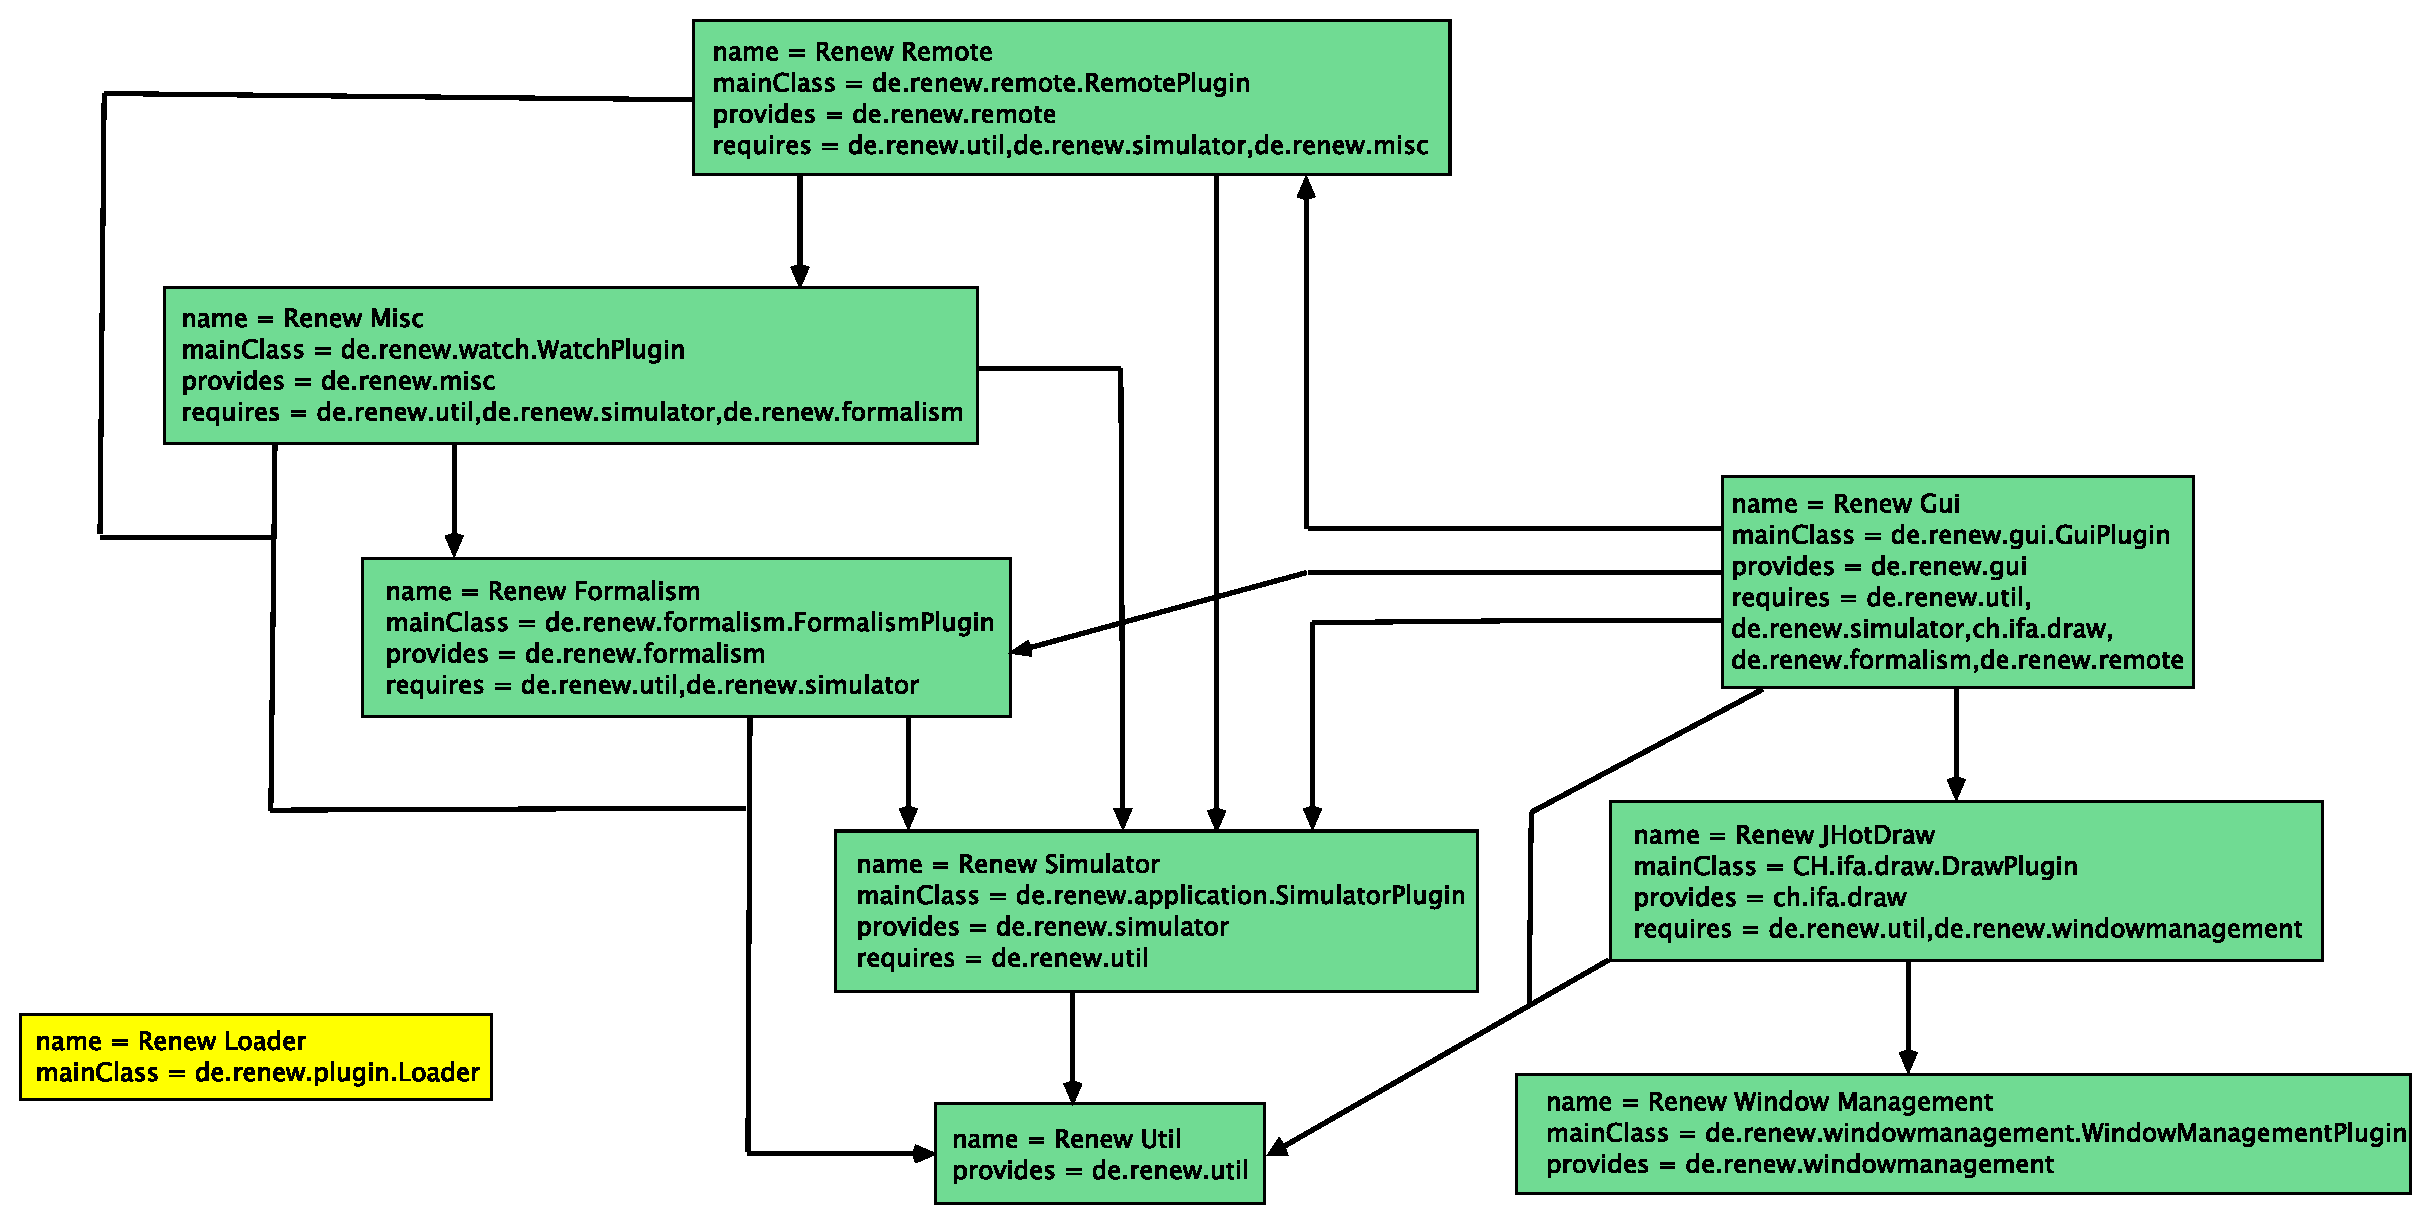
\includegraphics[width=\textwidth]{material/images/renew_plugin_dependencies2.pdf}
	  \caption{Gui Plugin-Abhängigkeiten}
	  \label{fig:plugin_deps}
	\end{figure}

	Für die Evaluation der minimalen Konfiguration starten wir aus dem \textit{Gui}-Plugin und arbeiten uns abwärts der Plugin-Hierarchie der \textit{plugin.cfg} hinab, bis der komplette Graph aufgebaut ist.\newline

	Die in der Abbildung \ref{fig:plugin_deps} repräsentierten Zusammenhängen reflektieren die von den Entwicklern abgestimmten Laufzeitabhängigkeiten, die einen groben Überblick über die nötigen Plugins verschaffen. Diese können zur Laufzeit alle benötigten Daten und Klassen enthalten, jedoch tragen sie keine Aussage über Abhängigkeiten während der Kompilation. Demgemäß kann zusätzlicher Code sowie Plugins benötigt werden. 


\subsection{Mulan} \label{sub:mulan}
	Mulan \cite{Roelke04} ist ein Multiagenten Rahmenwerk, mit dem Agenten entwickelt und mit einander verbunden werden können. Diese agieren nach eigenem Interesse und verhandeln über Kommunikationskanäle, die von Mulan angeboten werden. Um eine auf Mulan basierende Multi-Agent-Anwendung zu erstellen, müssen zahlreiche Protokollnetze gezeichnet und Wissensbasen erstellt werden, die das Verhalten und die Interaktion von Agenten implementieren. Somit bietet Mulan ein Kommunikationsplattform sowie ein Gerüst für die Umsetzung der darauf aufsetzenden Agenten und dessen Eigenschaften sowie Fähigkeiten, die mit Referenznetzen entworfen werden können. \cite{cabac} \bigbreak

	Das Spiel Settler ist mit Mulan umgesetzt und implementiert somit die Agenten Anforderungen des Multi Agenten System. Diese halten Wissensbasen über die Spielregeln und können mit Hilfe der Protokollnetze bestimmte Entscheidungen treffen und Handlungen ausführen. Wie zum Beispiel Straßen bauen oder Karten handeln.\bigbreak
	
	\begin{figure}[h!]
	  \centering
	  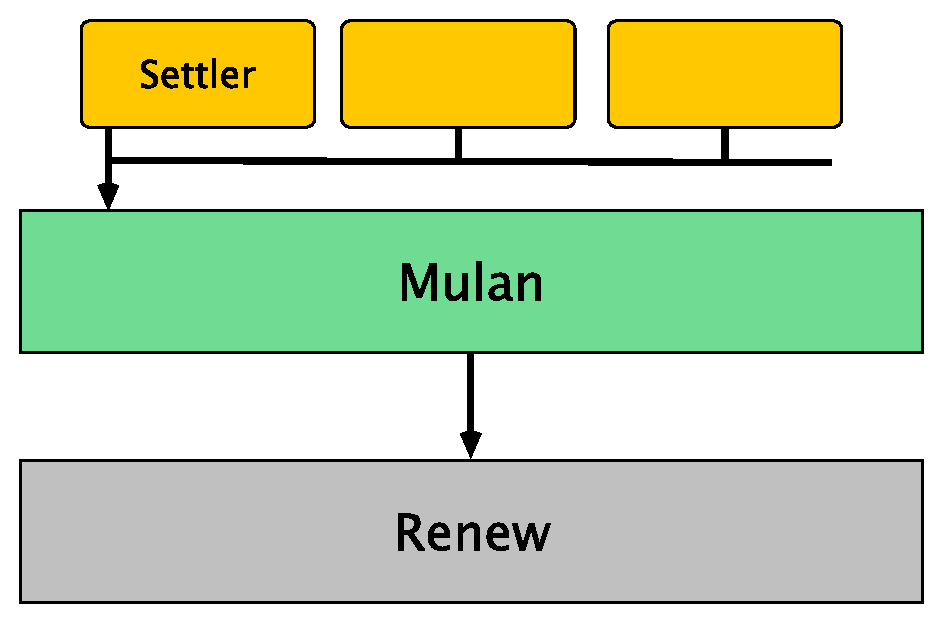
\includegraphics[width=0.5\textwidth]{material/images/settler-mulan-renew.pdf}
	  \caption{Mulan Plugins}
	  \label{fig:mulan_plugin}
	\end{figure}

	Damit die erstellten Settler Agenten und dessen Aufbau simuliert werden kann, wird der Renew Petrinetz Simulator verwendet, mit dem die umgesetzten Agenten-Strukturen betrieben werden können.\newline
	Des weiteren besitzt das Settler Spiel sowie das Mulan-Rahmenwerk eine Plugin konforme Architektur und werden somit genauso, wie die Renew Plugins von dem Renew Plugin-Manager ausgelesen und verwaltete.\bigbreak

	Eine vereinfachter Zusammenhang ist in der Abbildung \ref{fig:mulan_plugin} dargestellt und visualisiert die benötigten Grundlagen für die Ausführung von Settler.


\section{Durchführung} \label{sec:durchführung}
	Die wichtigen Szenarien für das erreichen des gesetzten Ziels werden mit zwei Prototypen umgesetzt. Der Renew Prototyp wird eine kontinuierliche  Modularisierung der Plugins und dessen Betriebsfähigkeit mit nur zum Teil Modularisierter Codebasis abdecken. Dazu gehört das Erstellen einer neuen Projektstruktur für die auserwählten Plugins und behandelt auserwählte Richtlinien, die mit dem Modulsystem von Java eingeführt worden sind. Für das Anfertigen von ausführbar Code, wird das Gradle Werkzeug integriert, das einen Kompilation Kontext für die neuen Module erstellt. Dazu gehört eine Abhängigkeitsverwaltung sowie Projektkopplung. Um die Plugins mit einender als Module zu verzahnen, werden Schnittellen untersucht und in der \textit{module-info} Konfigurationsdatei in den Plugins verankert. In der folgenden Evaluation wird das Ergebnis evaluiert und sauber Aufbereitet.\bigbreak 

	Im Gegensatz dazu behandelt der Mulan Prototyp die Zusammenführung bestehender Systeme mit modularisierten Code. Für die Umsetzung werden nur für das Spiel Settler relevanten Mulan Plugins erarbeitet und auf die minimale Renew Version aufgesetzt. Doch zuerst muss eine erweiterte Analyse der minimalen Renew Version durchgeführt werden, um die benötigten Renew Plugins für das Mulan Rahmenwerk nachzurüsten. Im weiteren Verlauf behandelt dieser Prototyp Konsequenzen der Umstellung auf eine neue Renew Grundlage und der benötigten Ausführungsschritte für die Adaption. Die Evaluation bewertet den Aufwand für die Umsetzung des Prototypen. 



 %	Die saubere Umsetzung behandelt den internen Aufbau, Namen- und Paketkonventionen sowie die Modulschnittstellen, die das Interagieren mit den Modulen einheitlich beschreiben und einen Vertrag mit den Nutzer eingehen. Zusätzlich muss der Inhalt eines Moduls klar festgelegt werden, da dieser nur einen Teil der zusammengesetzte Software abbildet und den Funktionsumfang beschränkt. \bigbreak 

 %Es müssen neue Konzepte integriert, Richtlinien befolgt und veraltete Konstrukte ersetze werde. Zu den genannten Problemen gehören Zyklen, Split-Packages und interne API-Zugriffe, die für den Umstieg sorgfältig gepflegt werden müssen.









\chapter{\textsc{Renew} Prototyp} 
	In diesem Kapitel entsteht ein Prototyp, der \textsc{Renew} schrittweise modularisiert, bis die Applikation den größten Teil ihre Funktionalität auf dem Modulpfad betreiben kann. \newline
	Für die Umsetzung des Prototypen werden zuerst Anforderungen erfasst, die der modularisierte \textsc{Renew} Prototyp erfüllen muss, um unserer Vision der Implementation zu entsprechen. Infolgedessen entsteht ein Implementierungsplan sowie ein Prototyp. 

\section{Anforderungen} \label{sec:anforderungen}
	Im Kern der Modernisierung von \textsc{Renew} liegt die Anpassung von \textsc{Renew} an das Modulsystem von Java und dessen Anforderungen an Applikationskomponenten. Aus den \textsc{Renew} Plugins sollen explizite Module entstehen, die auf dem Modulpfad betriebsfähig sein müssen. Die Drittanbieter-Bibliotheken sollen mit in den Modulpfad aufgenommen werden und als automatische Module ihre Aufgabe erfüllen. Zusätzlich darf die Migration und damit verbundene Anpassung und Aufbereitung der Mängel die Kommunikation sowie interne Funktionsweise von \textsc{Renew} nicht verändern. Dementsprechend soll garantiert werden, dass die darunter liegende theoretische Grundlage in Takt bleibt. 

% Was soll der Prototyp leisten 
\subsection{Interaktion}
	Der erste modulare \textsc{Renew} Prototyp soll mit einer minimalen Plugin Anzahl auf dem Modulpfad betriebsfähig sein und eine Möglichkeit bieten Petrinetze zu erstellen, zu simulieren und zu serialisieren. Das heißt, es muss eine UI zu sehen sein, die mit den nötigen Werkzeugen und der darunter liegender Logik ausgestattet ist. 

\subsection{Projektstruktur}
	Für die Umsetzung des modularen Renew's wird für jedes Plugin eine moderne Projektstruktur benötigt, die den Inhalt entsprechend dem etablierten Maven Standardverzeichnislayout auf Java Module und die dafür benötigten Ressourcen aufteilt. 

\subsection{Entwicklungsumgebung} 
	In der existierenden \textsc{Renew} Entwicklungsumgebung werden alle Plugin Projekte durch eine versteckte \textit{.project} beschrieben. Das heißt, der Klassenpfad und die Bindung der Codebausteine geschieht versteckt und für den Entwickler schwer zugänglich. Damit ist der Entwickler gezwungen den weiten und verschachtelten Weg durch die UI Konfiguration von Eclipse zu betreten, der sich mit der Zeit wandeln kann. Dieser Sachverhalt wurde von mir im letzten Projekt beobachtet und kostete Zeit für alle Projektteilnehmer, da die Universitätsrechner strikten Rechten unterliegen, die keine Benutzer definierte Eclipse Entwicklungsumgebung aufsetzen lässt. Darüber hinaus ist die Konfiguration von \textsc{Renew} in anderen Entwicklungsumgebungen wie IDEA oder Netbeans mit der \textit{.project} Konfigurationsdatei nicht möglich. \bigbreak

	Um eine Entwicklungsumgebung unabhängige Konfiguration anzulegen wird ein neues Werkzeug benötigt. 

\subsection{Packaging}
	Da \textsc{Renew} an das Modulsystem angepasst werden muss, muss die Prozedur für das Kompilieren  und das Verpacken der Codebasis die Veränderung miterleben.\newline
	\textsc{Renew} benutzt zurzeit das \textit{Apache Ant} Werkzeug, dass alle Plugins kompiliert und in eine ausführbare Form bringt. Dieses ist in Jahre gekommen und enthält wesentlich geringeren Funktionsumfang gegenüber der Aktuellen Konkurrenz, wie Maven und Gradle. Sie bieten eine Abhängigkeitsverwaltung, konfigurierbare Plugins und Programmiersprachen. Im Gesetz zu der aufgeblasenen XML-Konfiguration von Ant, die jeden kleinen Schritt ausführlich dokumentiert, beherrschen die modernen \textit{build} Werkzeuge die Komplexität durch den \textit{Convention over Configuration} Ansatz und flexiblen Ausdrucksweisen. \bigbreak

	Die minimale Version von \textsc{Renew} soll sich an einem modernen \textit{build} Werkzeug bedienen und ein ausführbares Ergebnis erzielen.

\section{Spezifikation}
	Um die Anforderungen umzusetzen, wird die erarbeitete minimale Version isoliert, umstrukturiert und mit dem Gradle \textit{build} Werkzeug für das Arbeiten in der Entwicklungsumgebung IDEA aufgerüstet. Da Gradle die Verwaltung des Projekts sowie das Kompilieren und Erstellen von ausführbaren Paketen übernehmen kann, ist es eine gute Wahl für das Aufsetzen einer modernen modularen Projektstruktur.\newline 
	Dafür muss das bestehende Ant \textit{build} System analysiert und mit dem Gradle Werkzeug wiederaufgebaut werden. Dieses soll so gut wie möglich die bestehende Drittanbieter-Bibliotheken verwalten, Module kompilieren und die benötigten Erweiterungen, wie das JavaCC Werkzeug, unterstützen.\bigbreak

	Nachdem die Projektstrukturen die passende Form angenommen haben, müssen die Projekt Abhängigkeiten analysiert und innerhalb der \textit{module-info.java} aufgenommen werden.\bigbreak

	Zu Letzt entsteht eine bekannte Ordnerstruktur mit Drittanbieter-Bibliotheken, Plugins und Konfigurationsdateien, die mithilfe des \textit{Plugin Manager} verwaltet werden.

\section{Entwurf}
	Der Entwurf berücksichtigt die schrittweise Migration und lässt die \textsc{Renew} Applikation während der Gesamtmigration betriebsfähig bleiben. Das heißt, Plugins auf den Klassenpfad sowie Modulpfad können nahtlos mit einander kommunizieren und ihre Funktion während der Migration weiterhin erfüllen.\bigbreak

	\begin{figure}[h!]
		\centering
		\begin{minipage}{7cm}
			\dirtree{%
			 .1 Project.
			 .2 src.
			 .3 main.
			 .4 java.
			 .5 de.application.purpose.
			 .6 de.
			 .7 application.
			 .8 purpose.
			 .4 resources.
			 }
		\end{minipage}
		\caption{Projektstruktur}
		\label{fig:projektstruktur}
	\end{figure}
	Für den ersten Prototypen wird zuerst eine Projektstruktur erstellt, die für jedes Plugin Projekt die Möglichkeit bieten soll, aus mehreren Modulen zu bestehen. Dafür wird eine Struktur \ref{fig:projektstruktur} erstellt, die im Java Verzeichnis alle Module bündelt, die über den Modulnamen disjunkt voneinander verwaltet werden. Nichtsdestotrotz gehören sie zum gleichen Projekt und teilen unter sich das Ressourcen Verzeichnis, das im weiteren Verlauf zum Erstellen der ausführbaren Pakete benötigt wird.\bigbreak
	       
	Nachdem die Projektstruktur der gewünschten Form entspricht, muss diese in der Gradle Konfigurationsdateien verankert werden. Hierfür wird für jedes Projekt die Projektstruktur und dessen Abhängigkeiten in der \textit{build.gradle} Konfigurationsdateien \ref{fig:gradle_project} festgehalten, indem Java sowie Ressourcen Stammverzeichnisse definiert und Projekte sowie Drittanbieter-Bibliotheken Abhängigkeiten für den Kompilation-Pfad bestimmen werden. \bigbreak

 		\begin{figure}[h!]
		\centering
		\begin{minipage}{7cm}
			\dirtree{%
			 .1 Project.
			 .2 build.gradle.
			 .2 settings.gradle.
			 .2 src.
			 .3 main.
			 .4 java.
			 .5 de.application.purpose.
			 .6 de.
			 .7 application.
			 .8 purpose.
			 .4 resources.
			 }
		\end{minipage}
		\caption{Gradle Konfiguration}
		\label{fig:gradle_project}
	\end{figure}
 	Die oben genannten Schritte müssen für jedes Projekt der minimalen Version von \textsc{Renew} durchgeführt und im Anschluss über die entsprechende Entwicklungsumgebung  validiert werden. Wenn diese alle Klassen und die benötigten Abhängigkeiten finden und kompilieren kann, wurden alle Projekte richtig strukturiert, definiert und mit einander sauber verbunden. In diesem Zustand ist die komplette Struktur des Projekts innerhalb von Gradle verpackt und kann von jeder Entwicklungsumgebung ausgelesen werden. \newline

	Da jetzt eine lauffähige minimale \textsc{Renew} Version für den Klassenpfad erstellt werden kann, ist es Zeit diese zu Modularisieren und die einzelnen Plugins auf den Modulpfad zu migrieren. Dafür werde ich den \textit{bottom up} Ansatz aus dem Kapitel Migration \ref{sec:bottomUP} verwenden und schritt für schritt die Plugins auf den Modulpfad bewegen.

	\begin{figure}[h!]
		\centering
		\begin{minipage}{7cm}
			\dirtree{%
			 .1 Project.
			 .2 build.gradle.
			 .2 settings.gradle.
			 .2 src.
			 .3 main.
			 .4 java.
			 .5 de.application.purpose.
			 .6 de.
			 .7 application.
			 .8 purpose.
			 .5 module-info.java.
			 .4 resources.
			 }
		\end{minipage}
		\caption{Modulumwandlung}
		\label{fig:module_project}
	\end{figure}

	Zuerst werden die Drittanbieter-Bibliotheken, wie \textit{log4j}, auf den Modulpfad als automatische Module eingebunden und werden damit aus den Klassen- sowie Modulpfaden für die Nutzung zugleich erreichbar sein. Anschließend werden Plugins als explizite Module migriert, die keine Plugin Abhängigkeiten besitzen und aus dem Modulpfad keine Zugriffe auf den Klassenpfad ausführen müssen.   Beispielsweise besitzt das \textit{Util} Plugin keine Abhängigkeiten auf \textsc{Renew} Plugins und wird für die Ausführung auf dem Modulpfad, durch eine \textit{moduel-info.java} Konfigurationsdatei erweitert. Wie in der Abbildung \ref{fig:module_project} dargestellt, muss sich diese im Stammverzeichnis des Moduls befinden und deklariert die benötigten automatischen Module.\newline
	In den nächsten Schritten werden Plugins Schritt für Schritt auf den Modulpfad migriert, indem für jedes Plugin eine eigene \textit{module-info.java} Konfigurationsdateien angelegt wird, in der sich ihre Abhängigkeiten auf automatische Drittanbieter-Module sowie explizite Plugin-Module befinden.\bigbreak 

	Dieses Vorgehen wird solange durchgeführt bis jedes Plugin sich auf dem Modulpfad befindet. 

\section{Umsetzung}

	Die Umsetzung realisiert den Entwurf und erstellt eine neue Projektstruktur für alle Plugins der minimalen \textsc{Renew} Version \ref{fig:plugin_deps}. Diese werden anschließend mit Gradle Werkzeug zusammengeführt und bilden ein kompilierfähiges Konstrukt. Nachfolgend werden die auserwählten Plugins, mit der \textit{module-info.java} versehen und deklarieren innerhalb der Konfigurationsdateien die zuvor vorgestellten Kommunikationskanäle \ref{sec:mod_kop} zwischen den Plugins.\newline
	Der Modularisierungsprozess geschieht iterativ und wird für jedes Plugin einzeln nacheinander durchgeführt.
\newpage
\subsection{Umstrukturierung}

	Für die Umsetzung der Anforderungen und des Entwurfs wird zuerst die Projektstruktur jedes Plugins angepasst. Dafür wird die Struktur jedes Plugins analysiert, umstrukturiert und im weiteren Verlauf von Mängeln befreit. In den meisten Fällen werden \textit{split pakages} und gemischte Strukturen innerhalb der Codebasis erwartet.\bigbreak
	Zuerst wird eine grobe Maven Projektstruktur erstellt, in dem sich zusätzlich ein Plugin Wurzelverzeichnis befindet. Anschließend migriert man die Codebasis in das Plugin Wurzelverzeichnis, welches den neuen Plugin Namen trägt.

	\begin{figure}[h!]
		\centering
		\small
		\setlength{\DTbaselineskip}{7pt}
		\begin{minipage}{7cm}
			\dirtree{%
			 .1 Gui.
			 .2 build.xml.
			 .2 etc.
			 .3 README.gui.
			 .3 plugin.cfg.
			 .2 src.
			 .3 de.
			 .4 renew.
			 .5 ant.
			 .5 gui.
			 .6 images.
			 .6 menu.
			 .6 pnml.
			 .7 converter.
			 .7 creator.
			 .7 parser.
			 .4 io.
			 .5 exportFormats.
			 .5 importFormats. 
			 }
		\end{minipage}
		\caption{Gui Projekt}
		\label{fig:gui}
	\end{figure}

	Das Gui Plugin enthält die geläufige mangelnde Organisation der Ressourcen. Zum Teil befinden sich diese in den \textit{etc} Verzeichnis und zum Teil sind diese in den Java \textit{source set} im \textit{images} Verzeichnis integriert, wie in der Abbildung \ref{fig:gui} dargestellt.\newline
	Um diese zu beheben, wird das Verzeichnis \textit{de.renew.gui.images}, das mit den \textit{png} und \textit{gif} Daten befühlt ist, in das Ressourcen Verzeichnis migriert. Damit die Applikation diese wiederfindet, werden die Zugriffspfade für die Ressourcen innerhalb des Gui Plugin an das neue Verzeichnis angepasst, indem die internen statischen Konstanten, wie \textit{CPNIMAGES}, auf den entsprechenden Ort verweisen. \newline
	Zum Schluss werden die \textit{README} und die \textit{plugin.cfg}  aus dem \textit{etc} Verzeichnis in das Ressourcen Verzeichnis bewegt. Somit ist eine Struktur erstellt worden, die sich auf das Modulsystem von Java anwenden lässt. \bigbreak

	\begin{figure}[h!]
		\centering
		\small
		\setlength{\DTbaselineskip}{7pt}
		\begin{minipage}{7cm}
			\dirtree{%
			 .1 Formalism.
			 .2 build.xml.
			 .2 etc.
			 .3 README.formalism.
			 .3 plugin.cfg.
			 .2 src.
			 .3 de.
			 .4 renew.
			 .5 formalism.
			 .6 base.
			 .6 bool.
			 .6 function.
			 .7 java.
			 .8 JavaNetParser.jj.
			 .7 pt.
			 }
		\end{minipage}
	  \caption{Formalism Projekt}
	  \label{fig:formalism}
	\end{figure}

	Andere Plugins wie Formalism, CH oder Misc besitzen \textit{JavaCC} Dateien, wie im Beispiel \ref{fig:formalism} dargestellt, enden diese auf \textit{jj}. Sie erstellen Java Netz Grammatiken und wandeln die Java-Basis für die Ausführung ab. Diese liegen lose zwischen den Java Klassen und werden von den Java Compiler nicht interpretiert. Daher macht es Sinn diese in ein eigens \textit{Source Set} auszulagern und für den JavaCC Compiler für die Übersetzung zu gruppieren.

	\begin{figure}[h!]
		\centering
		\footnotesize
		\setlength{\DTbaselineskip}{10pt}
		\begin{minipage}{.45\textwidth}
			\dirtree{%
			 .1 Formalism.
			 .2 src.
			 .3 main.
			 .4 java.
			 .5 de.renew.formalism.
			 .6 de.
			 .7 renew.
			 .8 formalism.
			 .9 base.
			 .9 bool.
			 .9 function.
			 .9 java.
			 .9 pt.
			 .4 javacc.
			 .5 JavaNetParser.jj.
			 .4 resources.
			 .5 README.formalism.
			 .5 plugin.cfg.
			 }
		\end{minipage}
		\begin{minipage}{.5\textwidth}
			\dirtree{%
			 .1 Gui.
			 .2 src.
			 .3 main.
			 .4 java.
			 .5 de.renew.gui.
			 .6 de.
			 .7 renew.
			 .8 gui.
			 .9 menu.
			 .9 pnml.
			 .10 conv.rng.
			 .10 converter.
			 .10 creator.
			 .10 parser.
			 .10 ptNetb.pntd.
			 .10 refNetb.pntd.
			 .9 io.
			 .10 exportFormats.
			 .10 importFormats.
			 .9 tasks.
			 .5 resources.
			 .6 README.gui.
			 .5 images.
			 .5 plugin.cfg.
			 }
		\end{minipage}
	  \caption{Resultierende Projektstrukturen}
	  \label{fig:resultStr}
	\end{figure}

	Das resultierende Resultat in der Abbildung \ref{fig:resultStr} erlaubt eine einfache Paketstruktur Analyse durchzuführen, um die \textit{Split Packages} zu identifizieren. \newline


	Auf den ersten Blick kann eine Überschneidung zwischen den Gui und den RenewAnt Plugin erkannt werden, da beide den \textit{de.renew.ant} Namensraum besetzen, der sich um bestimmte Ant spezifische Aufgaben kümmert. Aufgrund dessen wird der Namensraum in dem Gui Plugin in \textit{task} zu den Gunsten des RenewAnt Plugins umbenannt. Des Weiteren könnten beide \textit{Task's} in den RenewAnt Plugin verschoben werden, da dieser keine Abhängigkeiten in dem Gui Plugin besitzt und nicht in den Aufgabenbereich der UI fallen. 

\subsection{Gradle}

 	Um die Zyklen zu erkennen, wird ein Gradle \textit{build} Skript erstellt, der die Java \textit{Source Sets} für den Kompilation Schritt definiert und die benötigten Projekte sowie Drittanbieter-Bibliotheken auf den Projektklassenpfad einbindet. Mit der Unterstützung der Gradle Projektumgebung und einer IDE, können anschließend alle Abhängigkeiten aufgedeckt und auf Zyklen überprüft werden. \newline
 	Für die Umsetzung der Gradle Projektumgebung wird zuerst das bestehende Ant System analysiert. Dieses besteht aus Skripten, die sich in jedem Plugin befinden und die entsprechenden Projekte ausführbare Jar's erstellen. Die Ant Skripte sind sehr ähnlich aufgebaut und wiederholen ein Erstellungsmusster für alle Plugins. \newline
	\begin{figure}[h!]
	  \centering
	  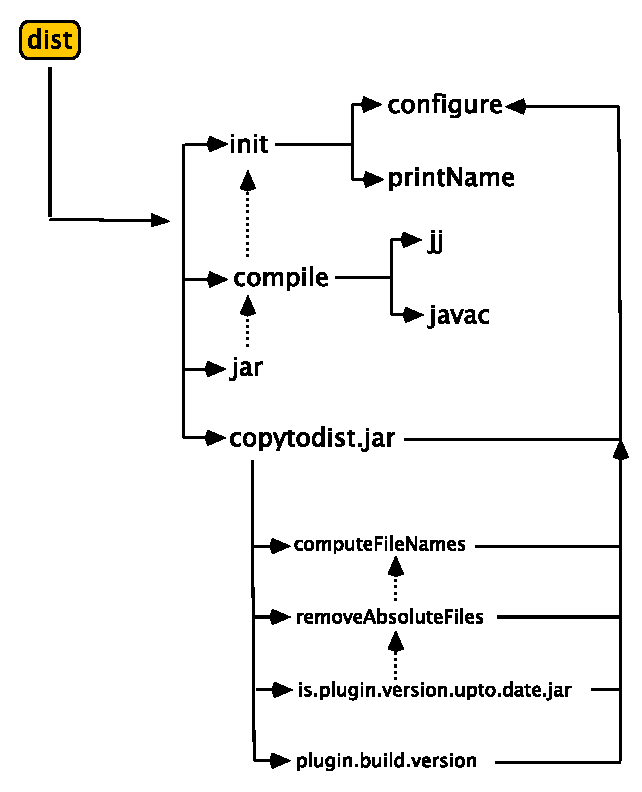
\includegraphics[width=0.5\textwidth]{material/images/ant-build.pdf}
	  \caption{Ant Skript}
	  \label{fig:antscript}
	\end{figure}

	In der Abbildung \ref{fig:antscript} ist ein Modell für die Erstellung eines Plugins mit dem Ant Werkzeug dargestellt. Ant initiiert das Skript mit Feldern und benötigten Variablen aus einer globalen Konfiguration, generiert Java Daten mit dem \textit{jj Target}, kompiliert und verpackt die ausführbaren Klassen. \bigbreak
	
	Für die Gradle Umsetzung werden Schritte, die über die etablierten Operationen zum Erstellen einer Ausführbaren Java Applikation wahrgenommen und in der folgenden Gradle Umgebung eingebunden.\newline
	Dafür wird zuerst ein übergeordneter Gradle Projekt deklariert, der Subprojekte aus allen Plugin Verzeichnissen erstellt.\bigbreak

	\begin{figure}[h!]
	  \centering
	  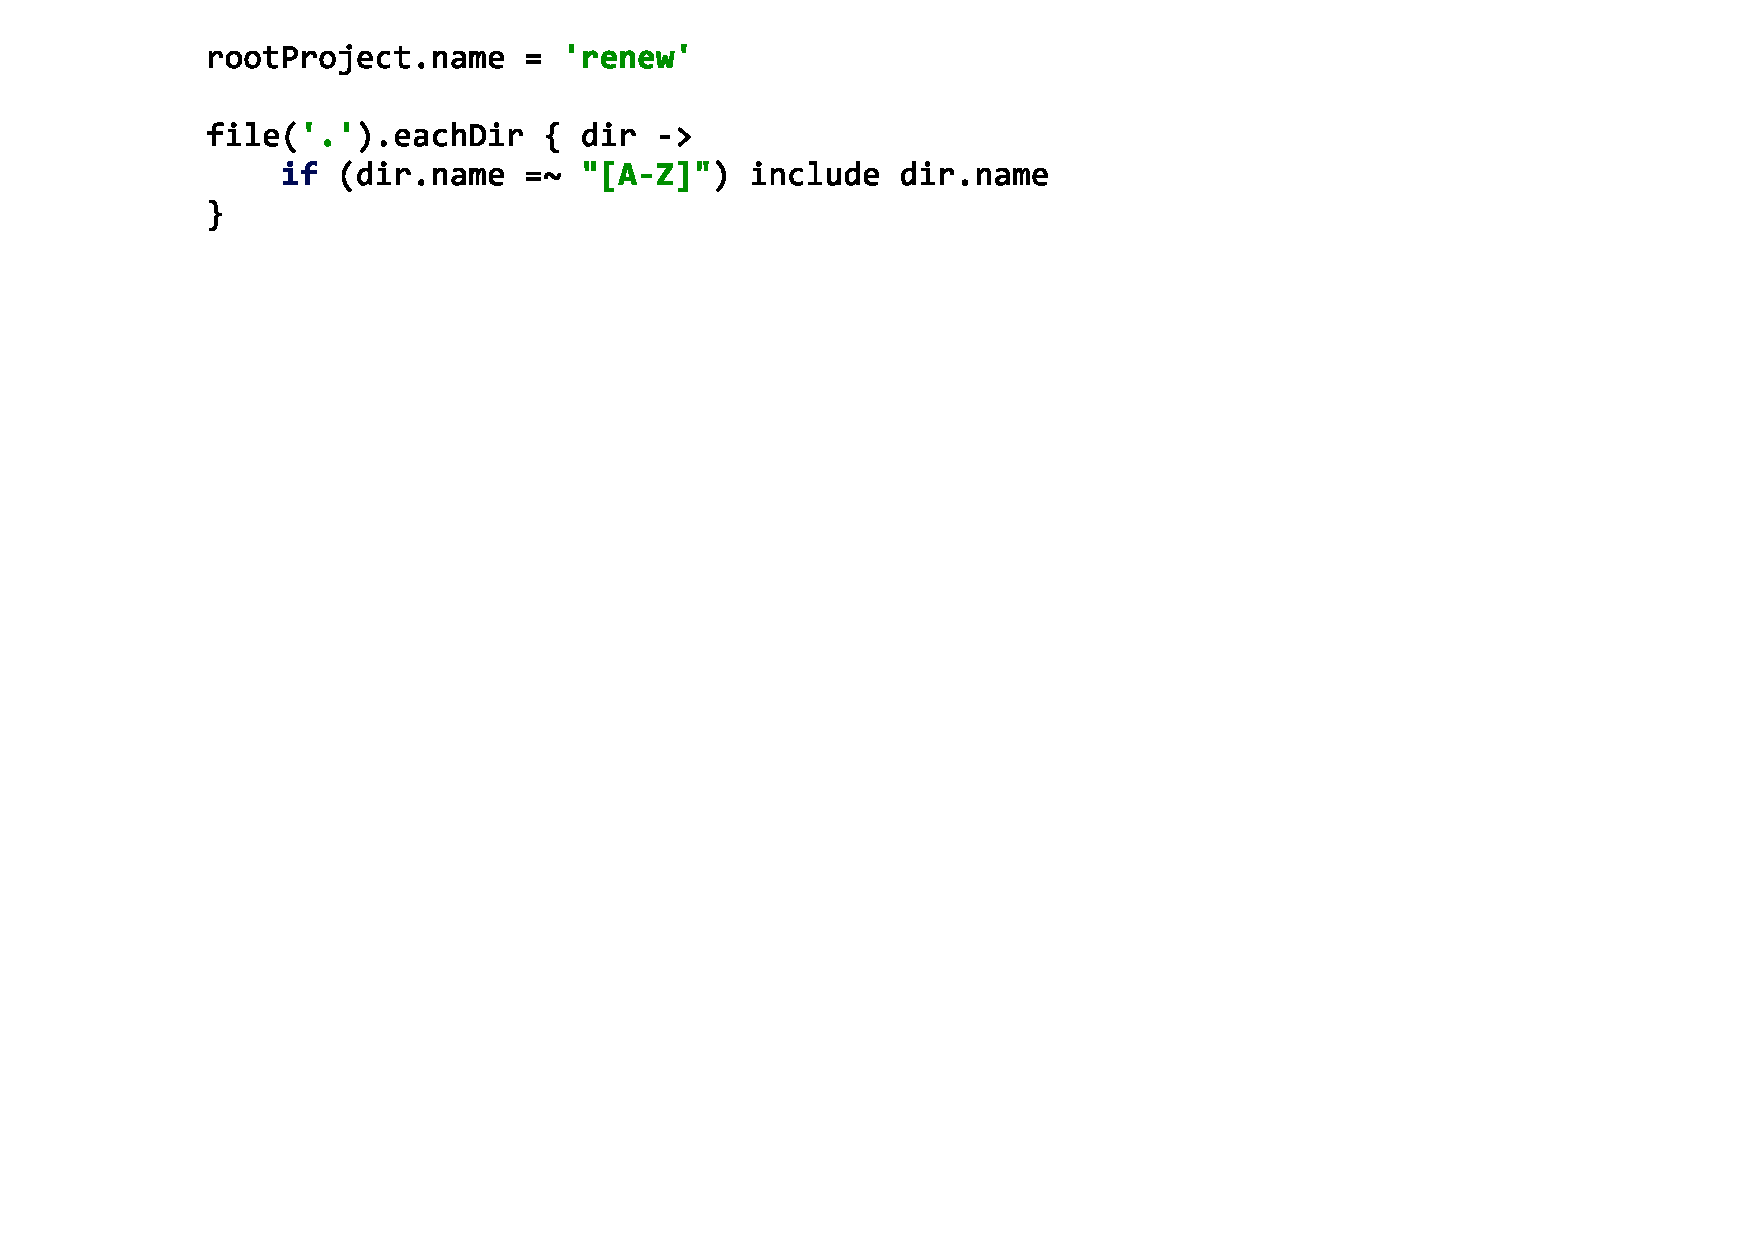
\includegraphics[width=0.6\textwidth]{material/images/settingsgradle.pdf}
	  \caption{Subprojekte}
	  \label{fig:subprojekte}
	\end{figure}

 	Die \textit{settings.gradle} Datei in der Abbildung \ref{fig:subprojekte}, die in der Konfigurationsphase des Gradle Lebenszyklus ausgelesen wird, ist für diesen Konfigurationsschritt zuständig und kann mithilfe von \textit{Groovy} beliebigen Code für die Deklaration der Projekte enthalten. In diesem Fall werden alle Verzeichnisse, die mit einem Großbuchstaben anfangen als Gradle-Subprojekte eingebunden.\bigbreak

	\begin{figure}[h!]
	  \centering
	  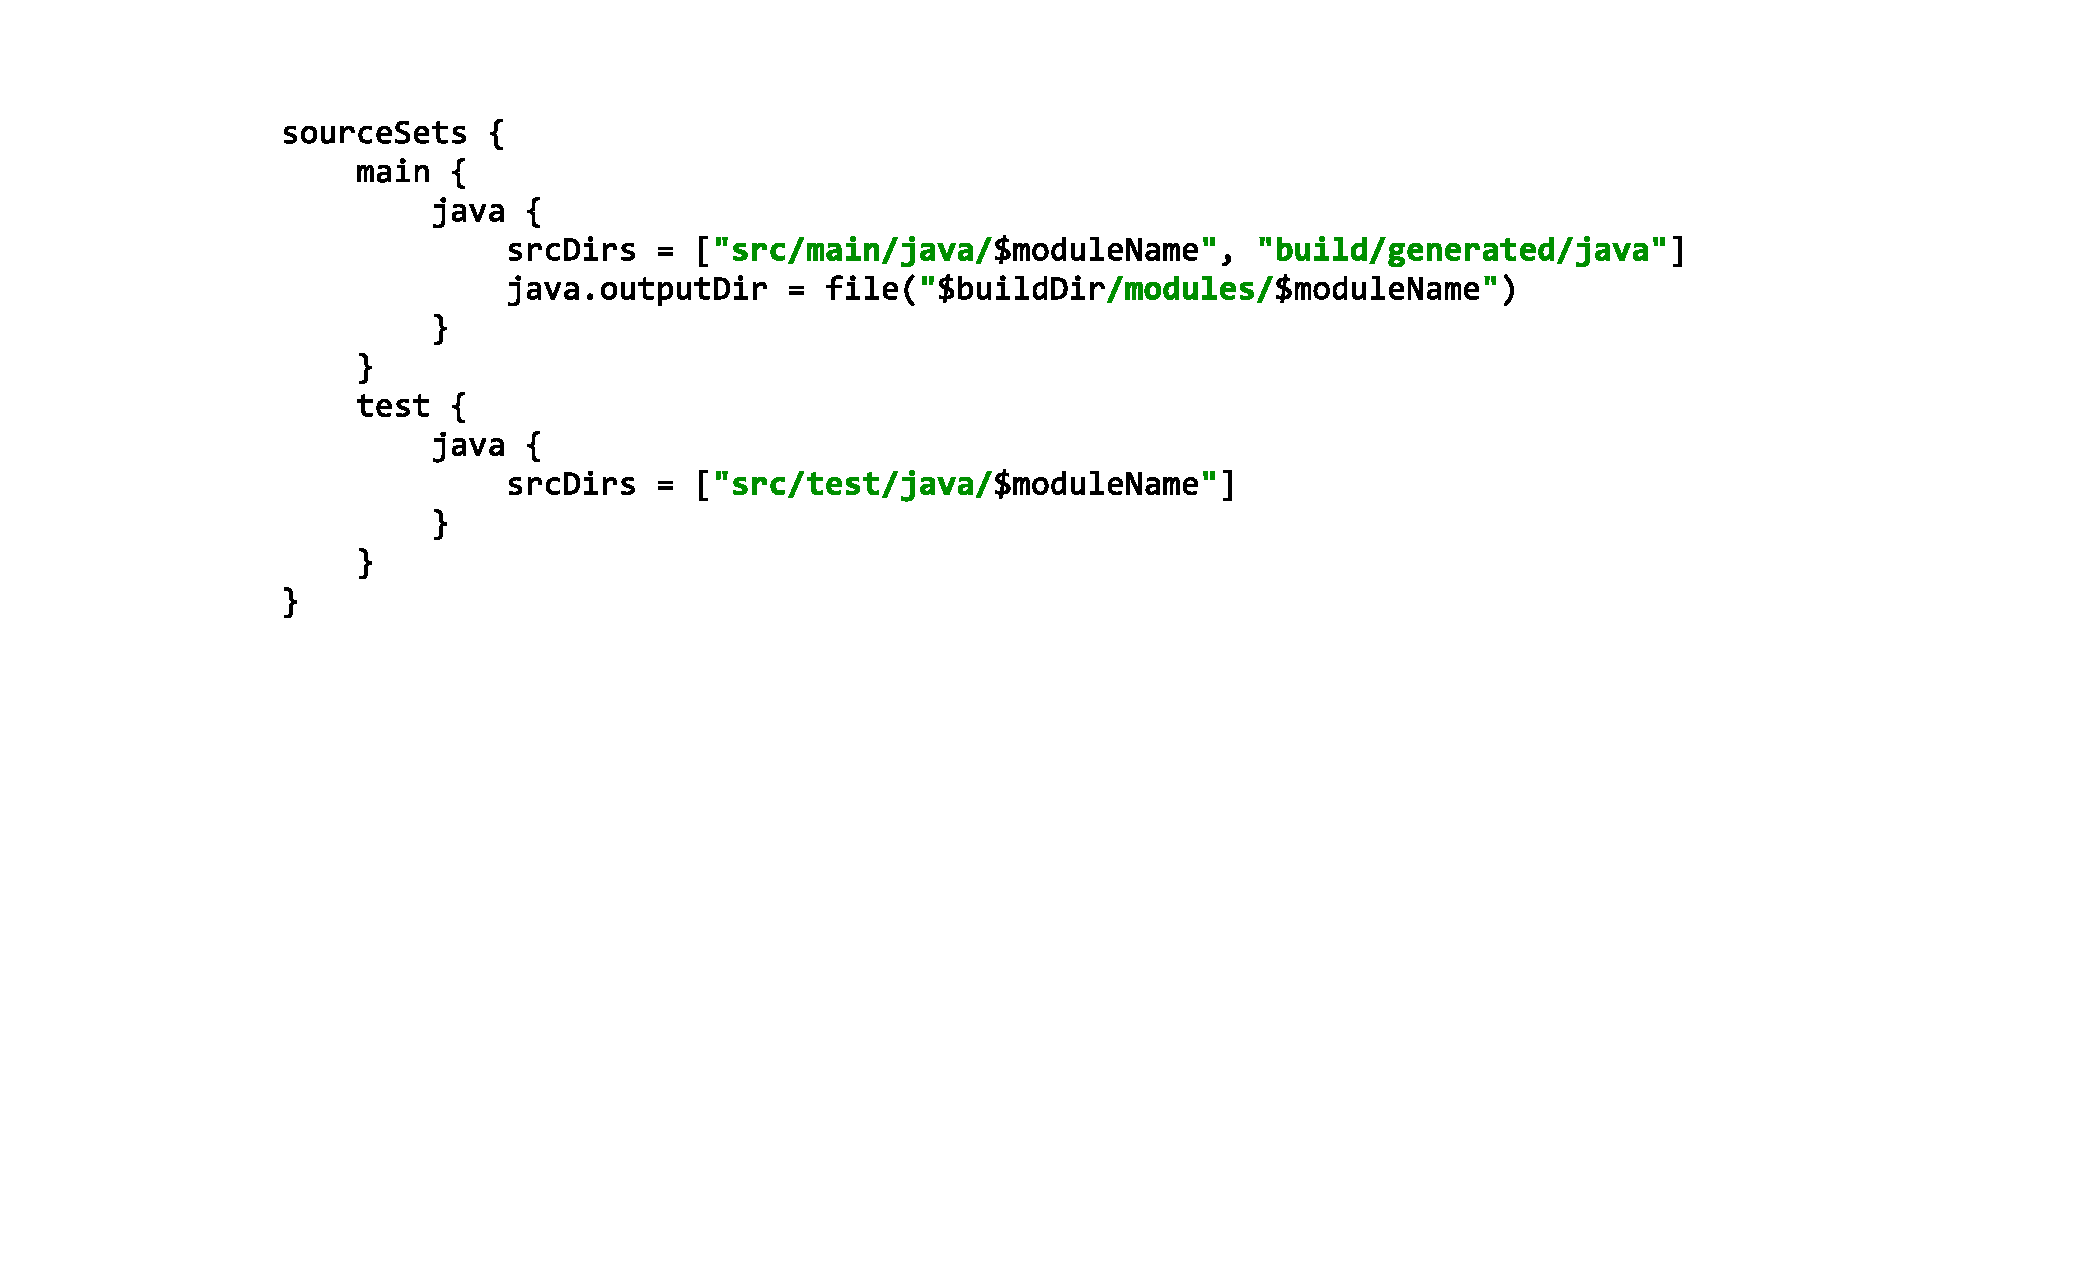
\includegraphics[width=0.7\textwidth]{material/images/sourcesets.pdf}
	  \caption{Source Sets}
	  \label{fig:Source_Sets}
	\end{figure}

 	Anschließend müssen die Java \textit{Source Sets} des Projekts bestimmt werden. Um die Umsetzung so einfach wie möglich zu gestalten, wird in der \textit{buld.gradle} Konfigurationsdatei, die für die Ausführungsphase zuständig ist, eine \textit{subprojects} Konfiguration angelegt, die für jedes Subprojekte die interne Projektstruktur definieren lässt. Diese beschreibt wo Verzeichnisse mit den Java Code und den dazugehörigen Ressourcen sich befinden sollen.\bigbreak

	\begin{figure}[h!]
	  \centering
	  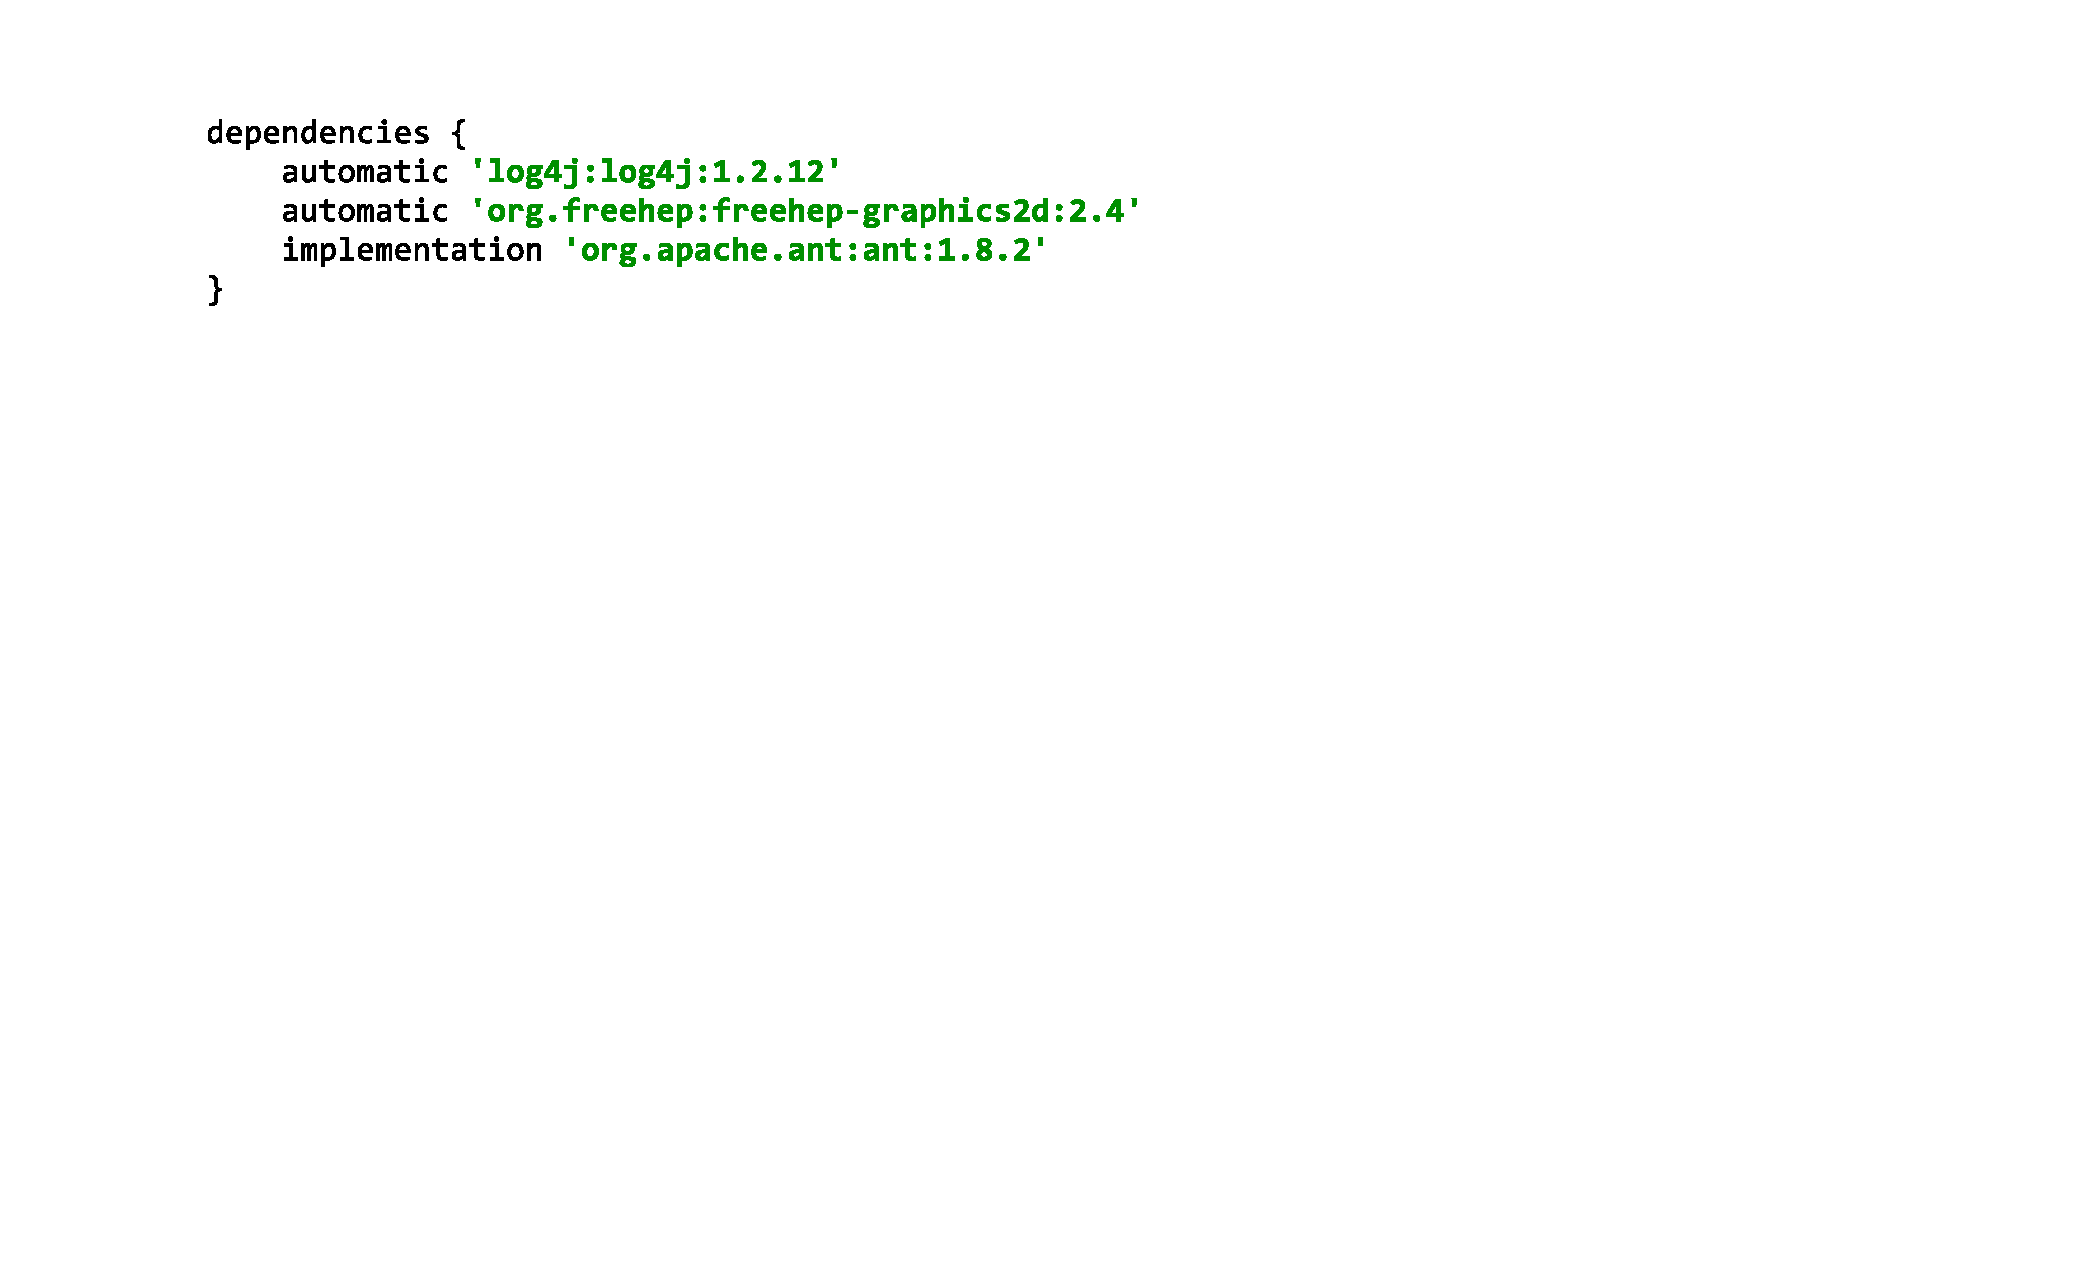
\includegraphics[width=0.6\textwidth]{material/images/gradle/dependencies.pdf}
	  \caption{Drittanbieter-Bibliotheken}
	  \label{fig:deps}
	\end{figure}

 	Im nächsten Schritt werden global genutzte Drittanbieter-Bibliotheken deklariert. Diese werden aus dem \textit{Maven Repository} beim initiiere des Projekts geladen und auf den Klassenpfad aller Plugin Projekte eingebunden. Somit liegt die Verwaltung der Bibliotheken und der dazugehörigen Version an den \textit{Maven Repository} und muss nicht mehr im \textit{GitLab Repository} bereitgestellt werden.\newline
 	Zusätzlich erleichtert die Deklaration der Drittanbieter-Bibliotheken, unter einer separaten Konfiguration, die Aufgabe der manuellen Erstellung der Klassenpfade und die Einbindung der Bibliotheken in der Entwicklungsumgebung, da die Konfiguration von der Entwicklungsumgebung automatisch aufgegriffen und auf das Projekt angewandt wird.\bigbreak

	\begin{figure}[h!]
	  \centering
	  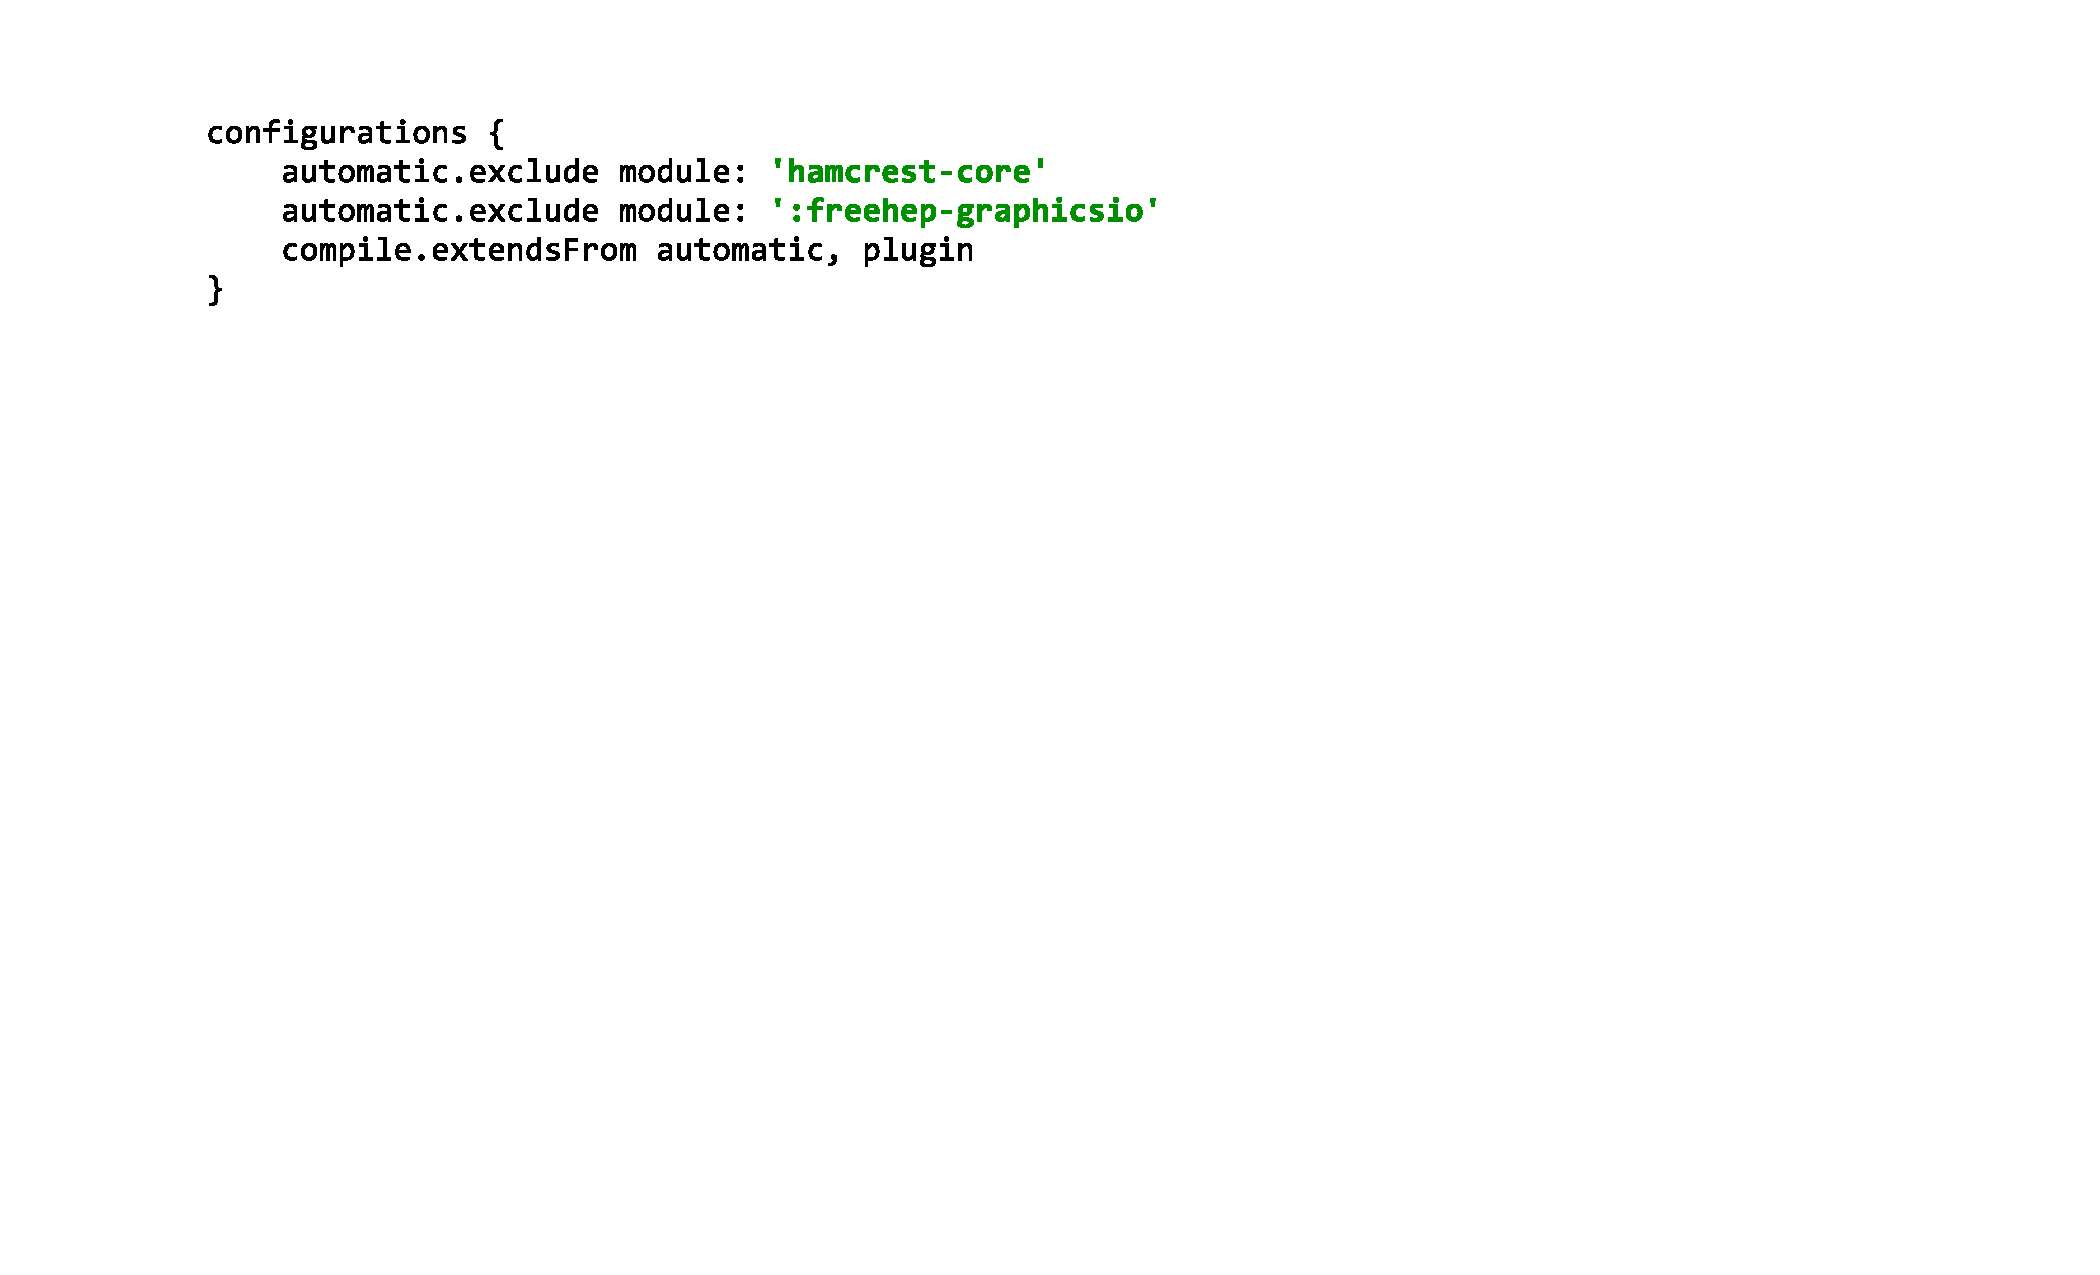
\includegraphics[width=0.6\textwidth]{material/images/gradle/configurations.pdf}
	  \caption{Klassenpfade}
	  \label{fig:kPath}
	\end{figure}

 	Um die Klassenpfade voneinander zu trennen werden zusätzliche Konfigurationen mit dem Namen \textit{plugin} und \textit{automaitc} eingeführt, die Plugin Code und Drittanbieter-Bibliotheken voneinander trennen und für das Kompilieren zusammenführen. Somit könne diese getrennt voneinander verwaltet, Modifiziert und bei Bedarf für bestimmte Aufgaben angepasst werden.\bigbreak

	\begin{figure}[h!]
	  \centering
	  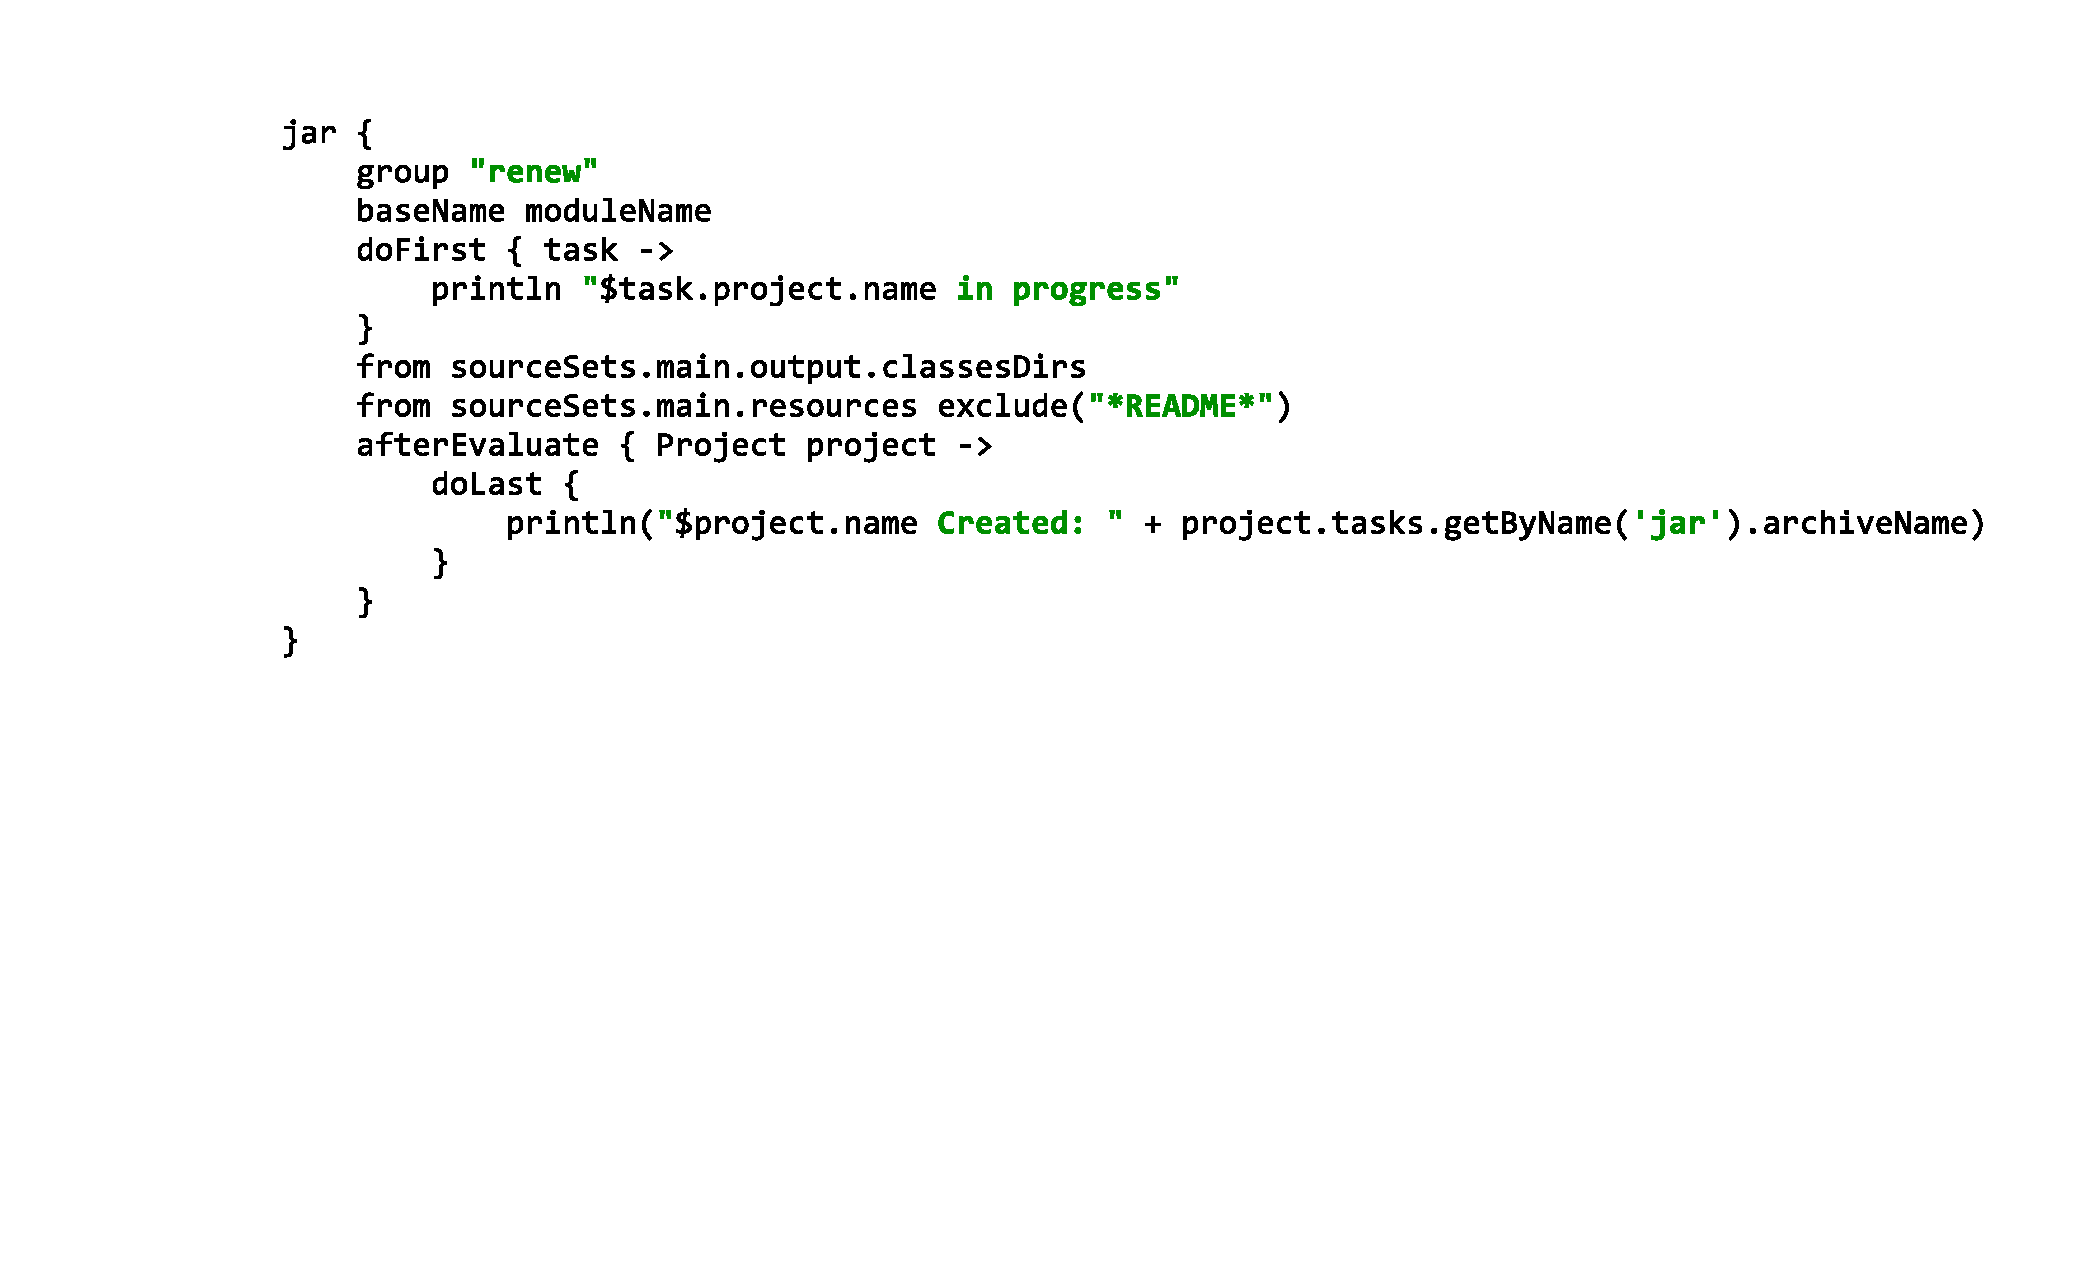
\includegraphics[width=\textwidth]{material/images/jar.pdf}
	  \caption{Jar Task}
	  \label{fig:jar}
	\end{figure}

	Zum Schluss der globalen Konfiguration wird ein \textit{jar} Task angelegt, der für ein gegebenes \textit{Source Set} ein \textit{jar}-Archiv für jedes Plugin mit den dazugehörigen Ressourcen erstellt.\newline
	Damit ist die globale Konfiguration der \textsc{Renew} Plugins beendet und bereit für die individuelle Anpassung der Plugin Bedürfnisse.\bigbreak

	\begin{figure}[h!]
	  \centering
	  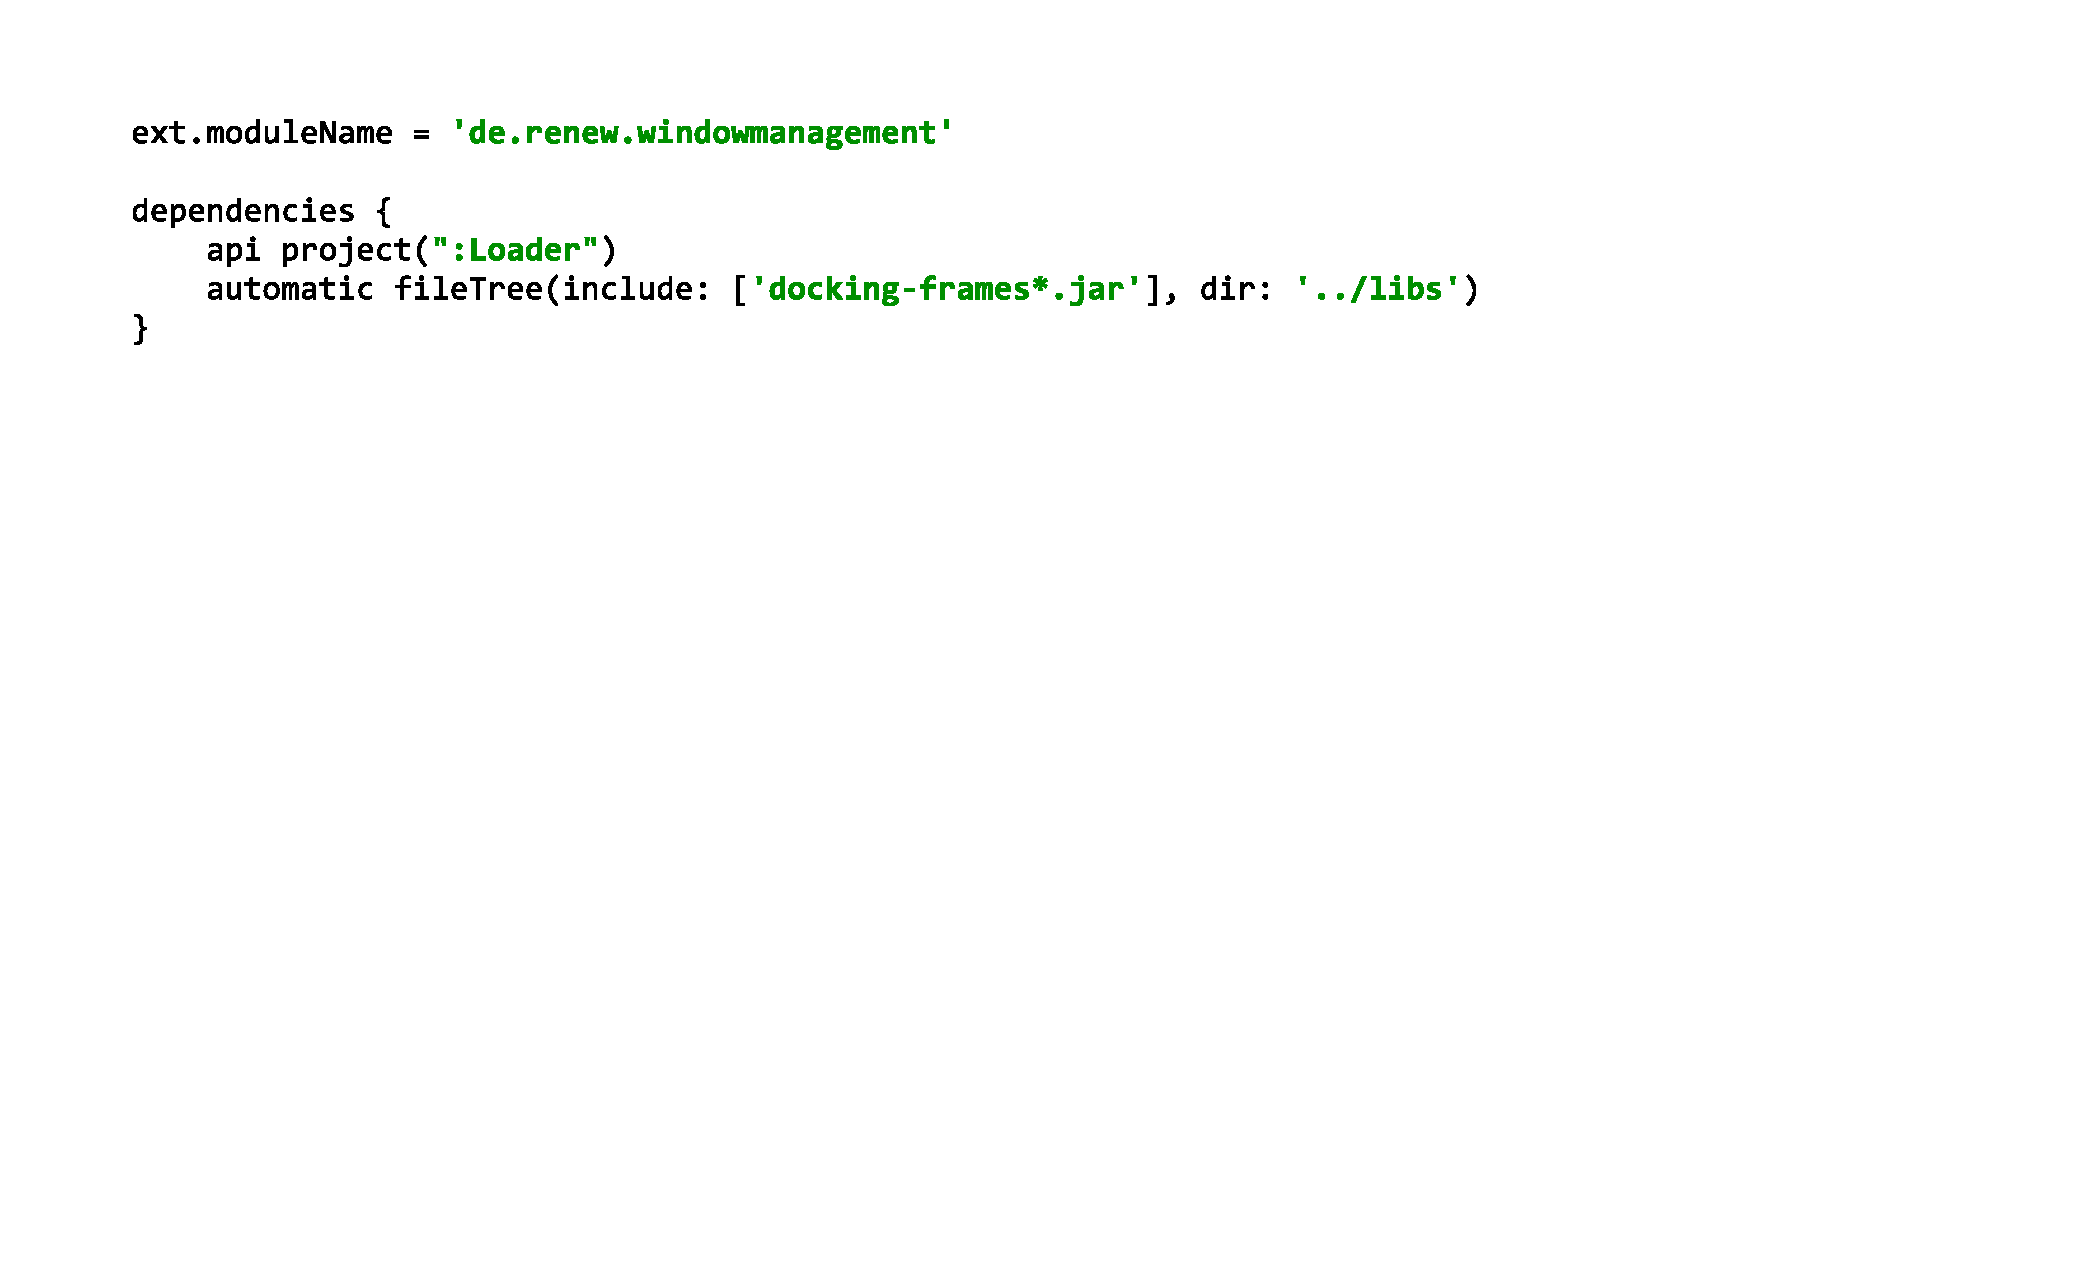
\includegraphics[width=0.8\textwidth]{material/images/gradle/winmangradle.pdf}
	  \caption{Individuelle Konfiguration}
	  \label{fig:windmang}
	\end{figure}

	Jedes einzelne Plugin benötigt einen internen Namen für die Verwaltung und die zusätzlichen Drittanbieter-Bibliotheken sowie Plugin Abhängigkeiten. Dafür wird in der Plugin \textit{buidl.gradle} Konfigurationsdatei der Name unter den \textit{extension properties} deklariert und die bereits geerbten Abhängigkeiten erweitert. In der Abbildung \ref{fig:windmang} wird das WindowManagment Plugin durch eine lokale, modifizierte Drittanbieter-Bibliotheken und durch das Plugin Projekt erweitert, um alle Benötigen Abhängigkeiten abzudecken.\bigbreak

	\begin{figure}[h!]
	  \centering
	  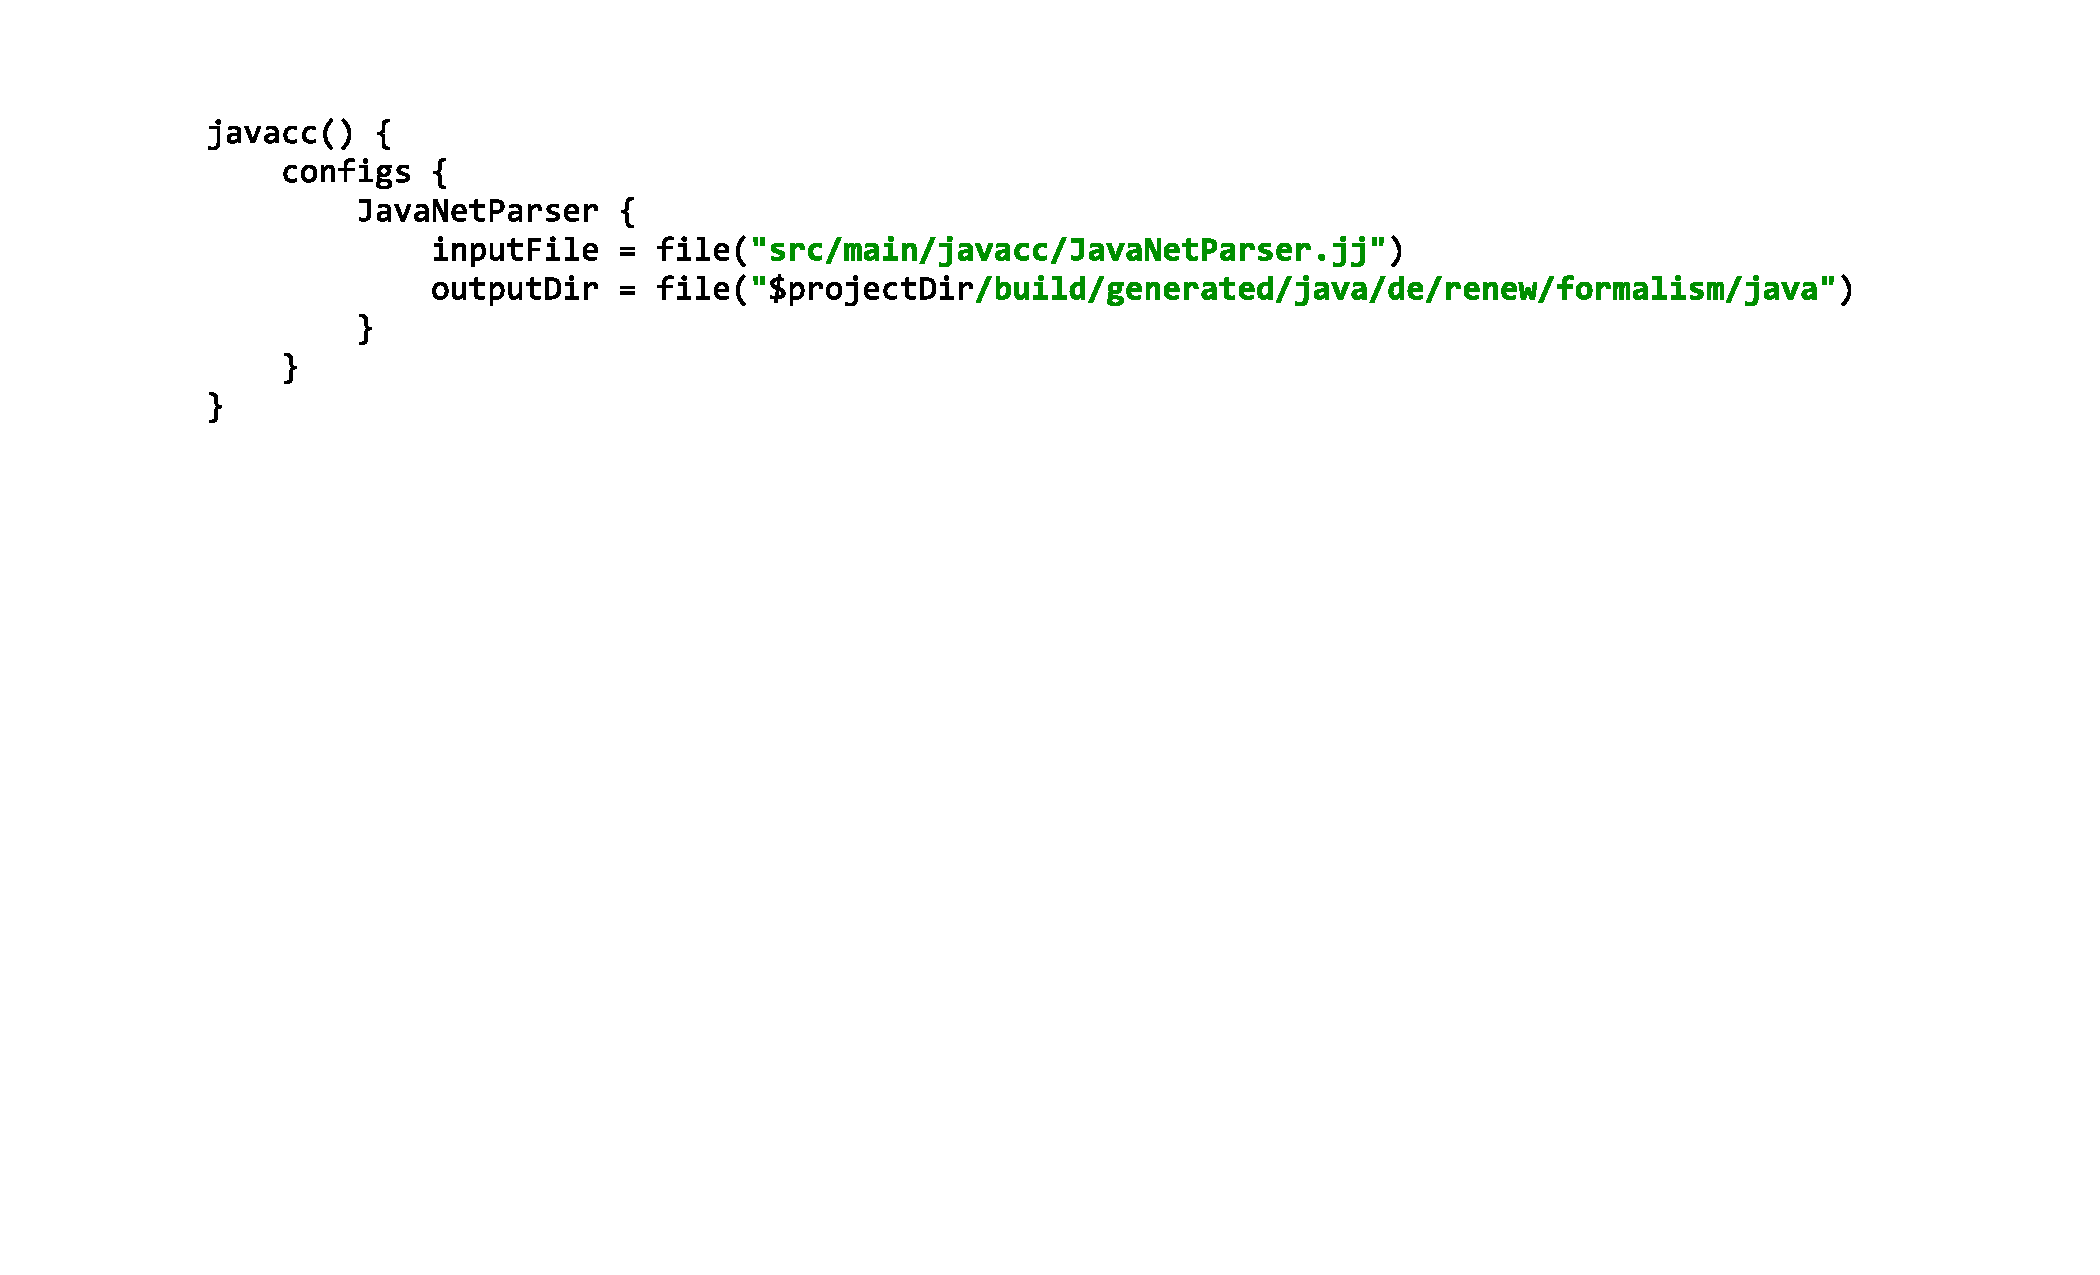
\includegraphics[width=\textwidth]{material/images/gradle/javacc.pdf}
	  \caption{Java Compiler Compiler}
	  \label{fig:javacc}
	\end{figure}

	Für die Konfiguration der einzelnen Plugins spielt der \textit{JavaCC} Parser eine große Rolle, denn dieser wandelt eine Grammatikspezifikation in ausführbaren Java Code um. Die genannte Technik wird in dem \textit{Formalism}, \textit{Feature Structures}, \textit{CH} und in dem \textit{Misc} Plugin verwendet. Der \textit{JavaCC} Parser erstellt Java Klassen, die obligatorisch für die Ausführung von \textsc{Renew} sind. Dementsprechend werden diese als generierte Ressourcen im \textit{build} Verzeichnis abgelegt und dem Java \textit{SourceSet} beigefügt. \bigbreak

	Jedes einzelne Plugin wird auf diese Weise konfiguriert und enthält einen Namen sowie zusätzliche Abhängigkeiten. Hiermit ist die Vorbereitung für die Modularisierung abgeschlossen. 


\subsection{Modularisierung}	
	Nachdem alle benötigen \textsc{Renew} Plugins kompiliert, verpackt und ausgeführt werden können, müssen die neu entstandenen Abhängigkeitsbeziehungen analysiert werden. Die Analyse der Plugins geschieht nun über die erstellten Gradle Scripte, die für jedes Projekt die benötigten Bibliotheken und Projekte für die Kompilation deklarieren. Aus diesen wird anschließend ein Abhängigkeitsgraph erstellt, der Zyklen und versteckte Abhängigkeiten offenlegt. \bigbreak

	\begin{figure}[h!]
	  \centering
	  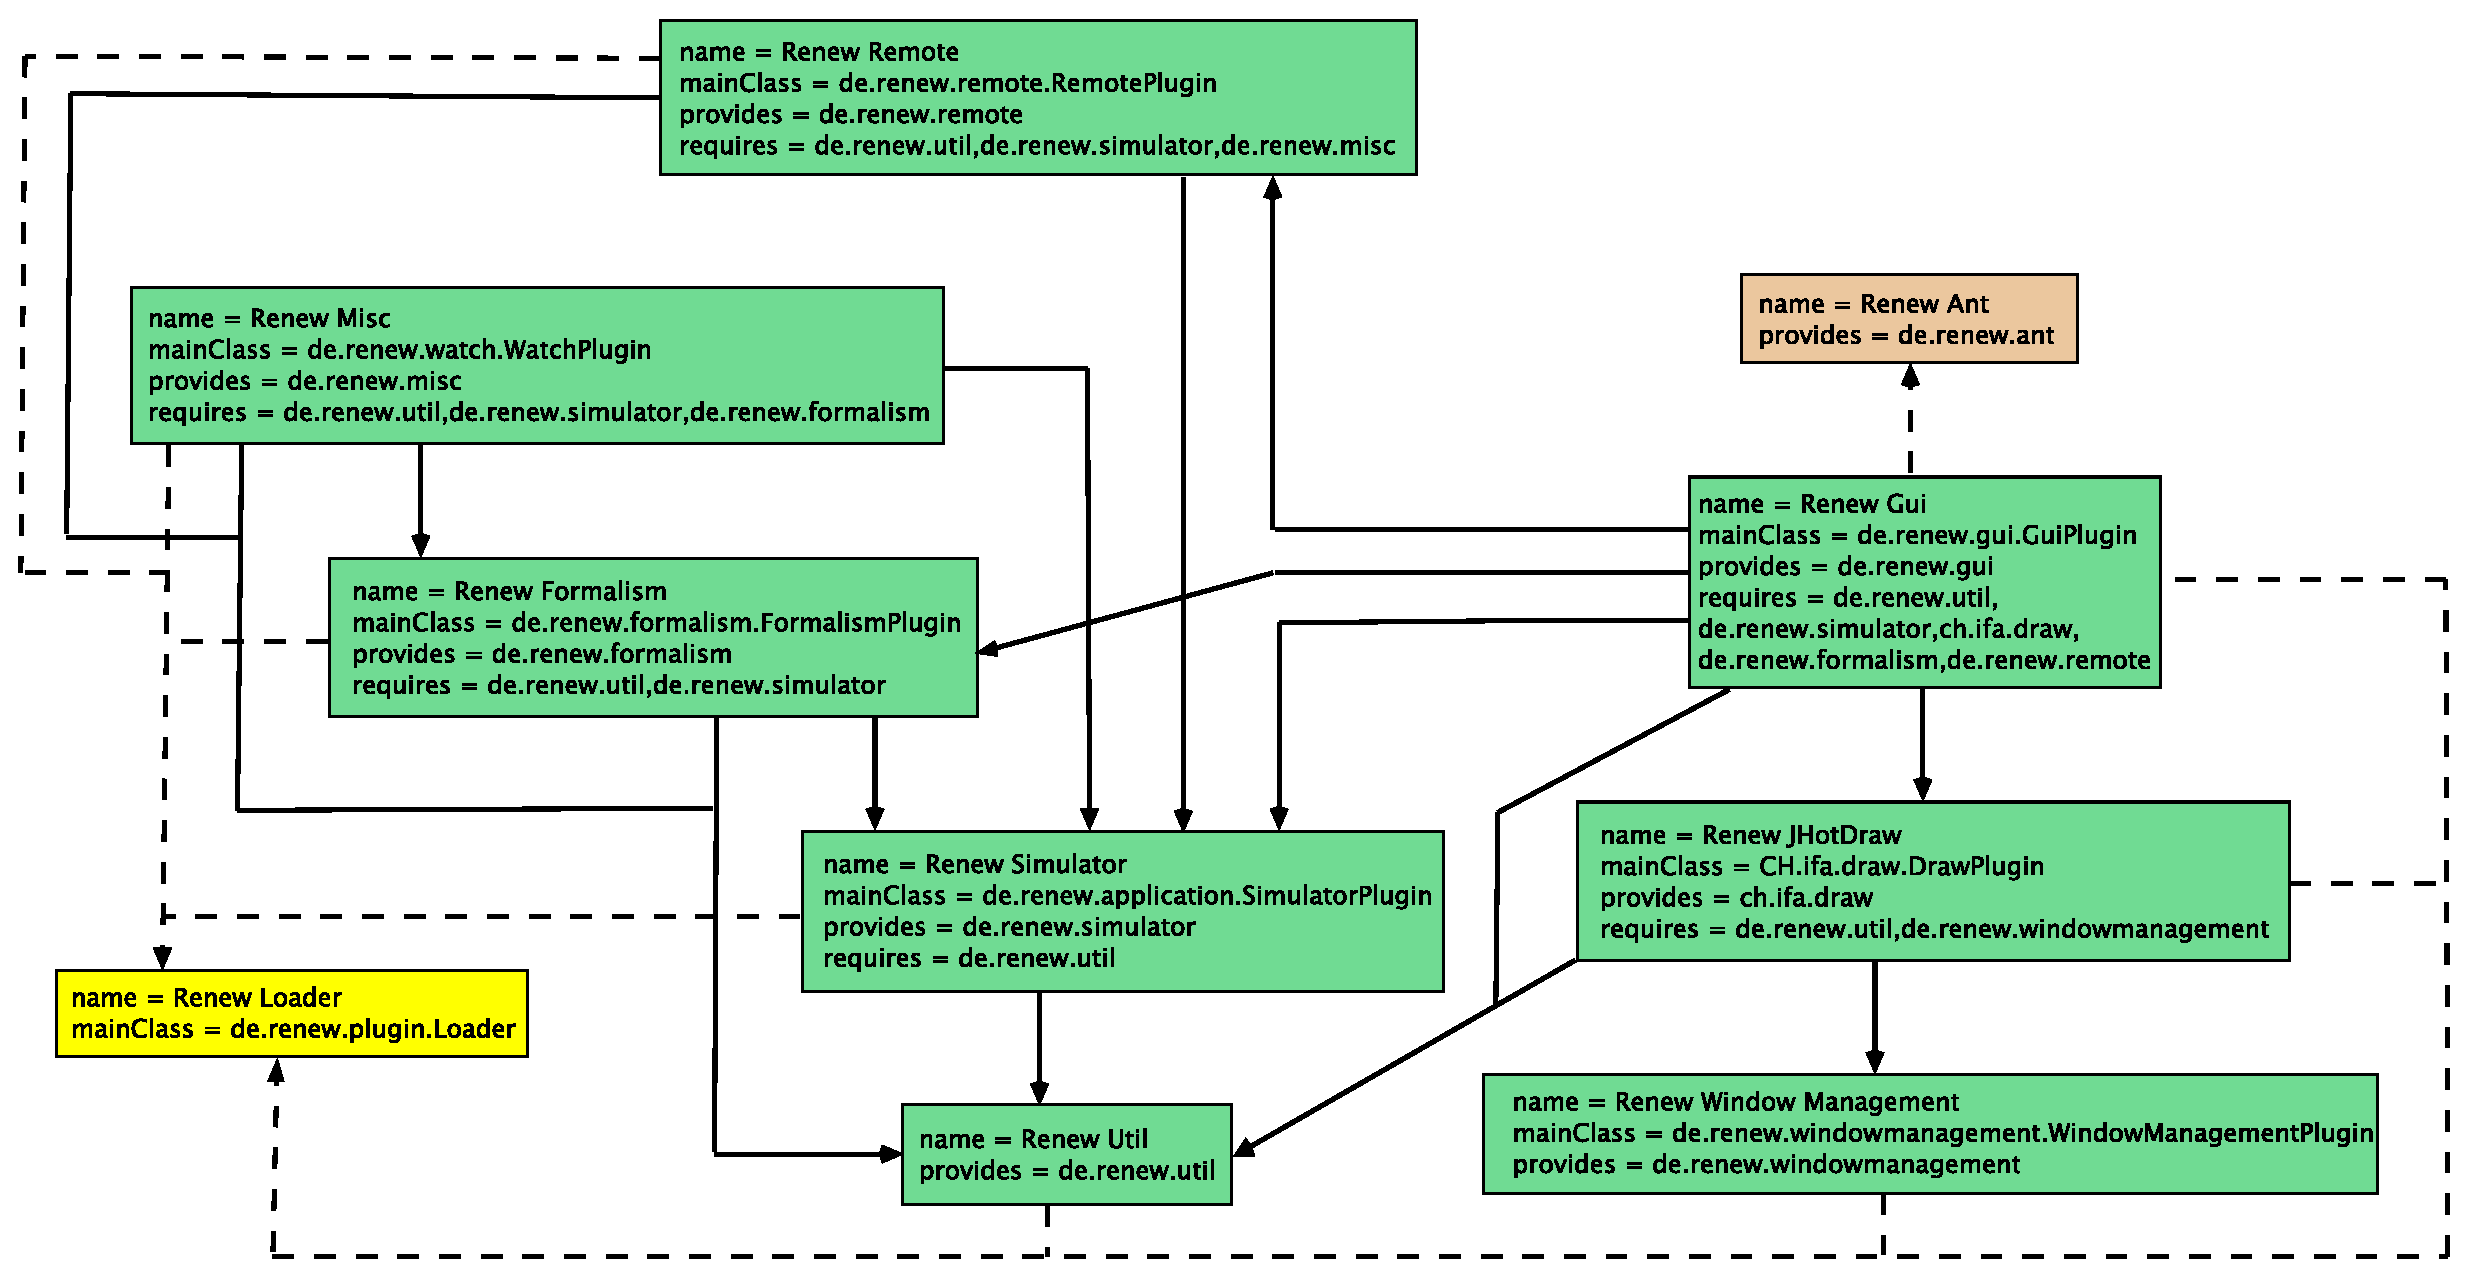
\includegraphics[width=\textwidth]{material/images/renew_plugin_dependencies-module-info.pdf}
	  \caption{Kompilation Abhängigkeiten}
	  \label{fig:deps}
	\end{figure}

	Der neu entstandene Graph wurde im Vergleich zu dem Graphen aus dem Ausgangssituation Abschnitt \ref{fig:plugin_deps} durch ein Plugin erweitert und bindet alle Plugins an das \textit{Loader} Projekt. Des Weiteren sind auf der Abbildung \ref{fig:deps} keine Zyklen in der minimalen Version zu beobachten und dementsprechend müssen auch keine weiteren Anpassungen durchgeführt werden. \bigbreak

	Die Migration von der minimalen Version von \textsc{Renew} wird von den \textit{Loader, Util} und \textit{Windowmanagment} Plugin eingeleitet. Diese besitzen keine Abhängigkeiten innerhalb der Plugin Menge und brauchen keinen Zugriff auf den Klassenpfade nachdem sie sich auf dem Modulpfad befinden. Im Gegensatz dazu, behalten Plugins, die sich auf dem Klassenpfad befinden und als ein unbenanntes Modul interpretiert werden, alle Zugriffsrechte auf die interne Struktur migrierten Plugins, wie bereits in den Abschnitt \ref{fig:modacc} beschrieben wurde.\bigbreak

	Da ein Modul seine eigne Abhängigkeiten verwalten muss, wird für jedes Plugin eine \textit{module-info.java} Konfigurationsdatei angelegt, die alle Java internen sowie Drittanbieter Bibliotheken auflistet. Für die ersten Module werden die erforderlichen Bibliotheken inklusive dem Loader Plugin in der Konfigurationsdatei mit dem Schlüssel \textit{requires} verankert und die dazugehörigen Drittanbieter-Bibliotheken aus den Klassenpfad auf dem Modulpfaden als automatische Module aufgesetzt.

	\begin{figure}[h!]
	  \centering
	  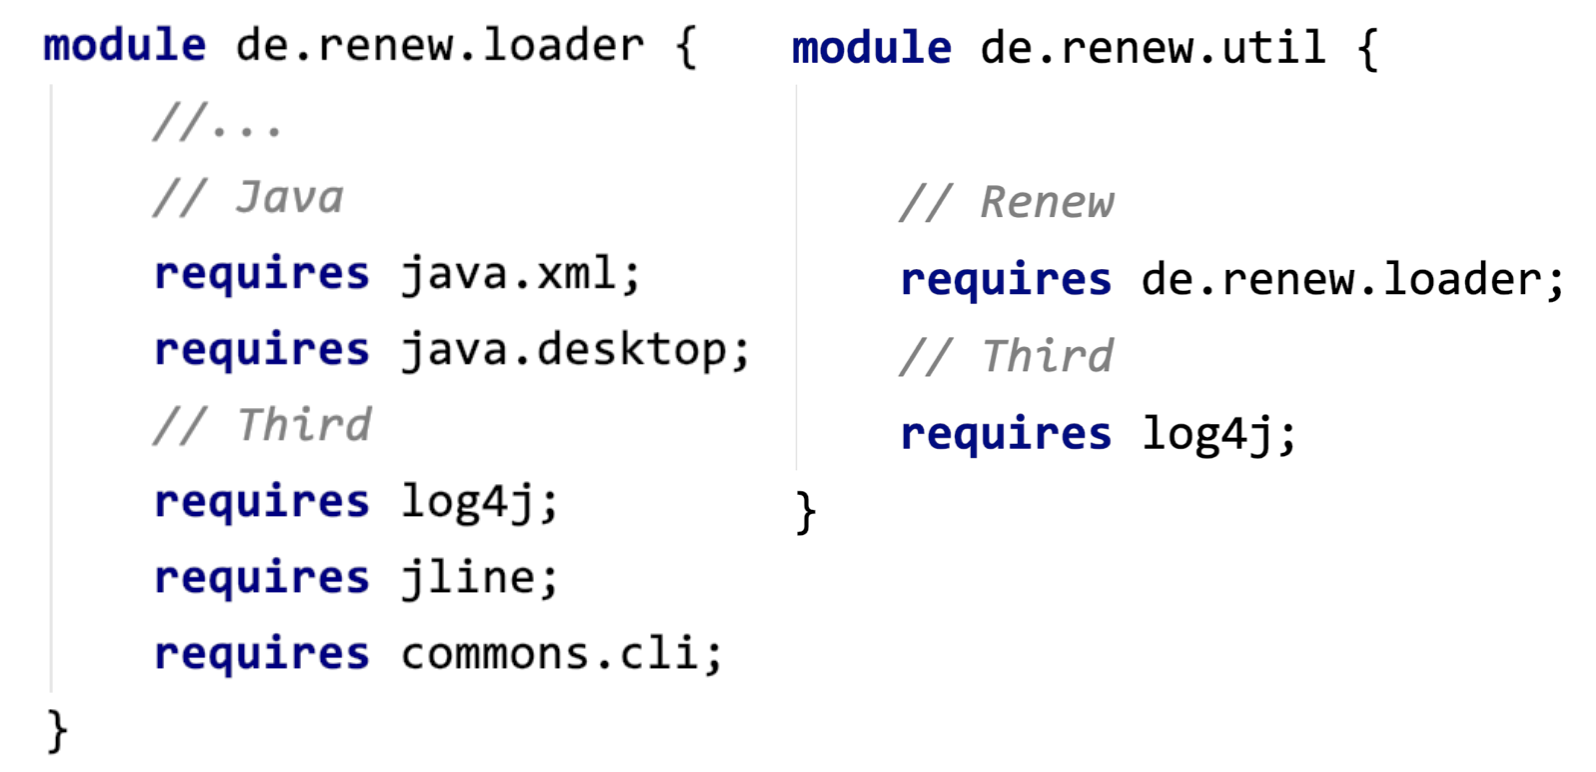
\includegraphics[width=0.7\textwidth]{material/images/loaderUtil-info.png}
	  \caption{Benötigten Bibliotheken}
	  \label{fig:loaderUtil}
	\end{figure}

	In diesem Zustand wird \textsc{Renew} kompiliert und ausgeführt. Das Ergebnis ist eine lauffähige Applikation, die ihre vollständige Funktion zugleich aus dem Modul- und Klassenpfad bezieht und identisch zu der initialen minimalen Version von \textsc{Renew} funktioniert.\newline
	Im nächsten Schritt werden Plugins migriert, die nur auf die neu entstandenen Module aufsetzen, wie zum Beispiel das \textit{Simulator} und das \textit{JHotDrow} Plugins. Ihre Abhängigkeiten liegen auf dem Modulpfaden, daher gibt es keinen Grund mit dem Klassenpfad zu interagieren. \newline
	Da diese die zweite Modulschicht repräsentieren, fordern sie bestimmte Funktionalität mit dem \textit{requiers} Schlüssel aus den Loader, Util und Windowmanagment Plugins. Um diese Anforderung zu entsprächen, müssen die notwendigen Plugins ihre Pakete  explizit für ihre Nutzer öffnen. Dazu deklarieren die angeforderten Plugins in ihrer \textit{module-info.java} mit dem \textit{exports} Schlüssel Pakte, die sie für andere Plugins zur Verfügung stellen möchte.

	\begin{figure}[h!]
	  \centering
	  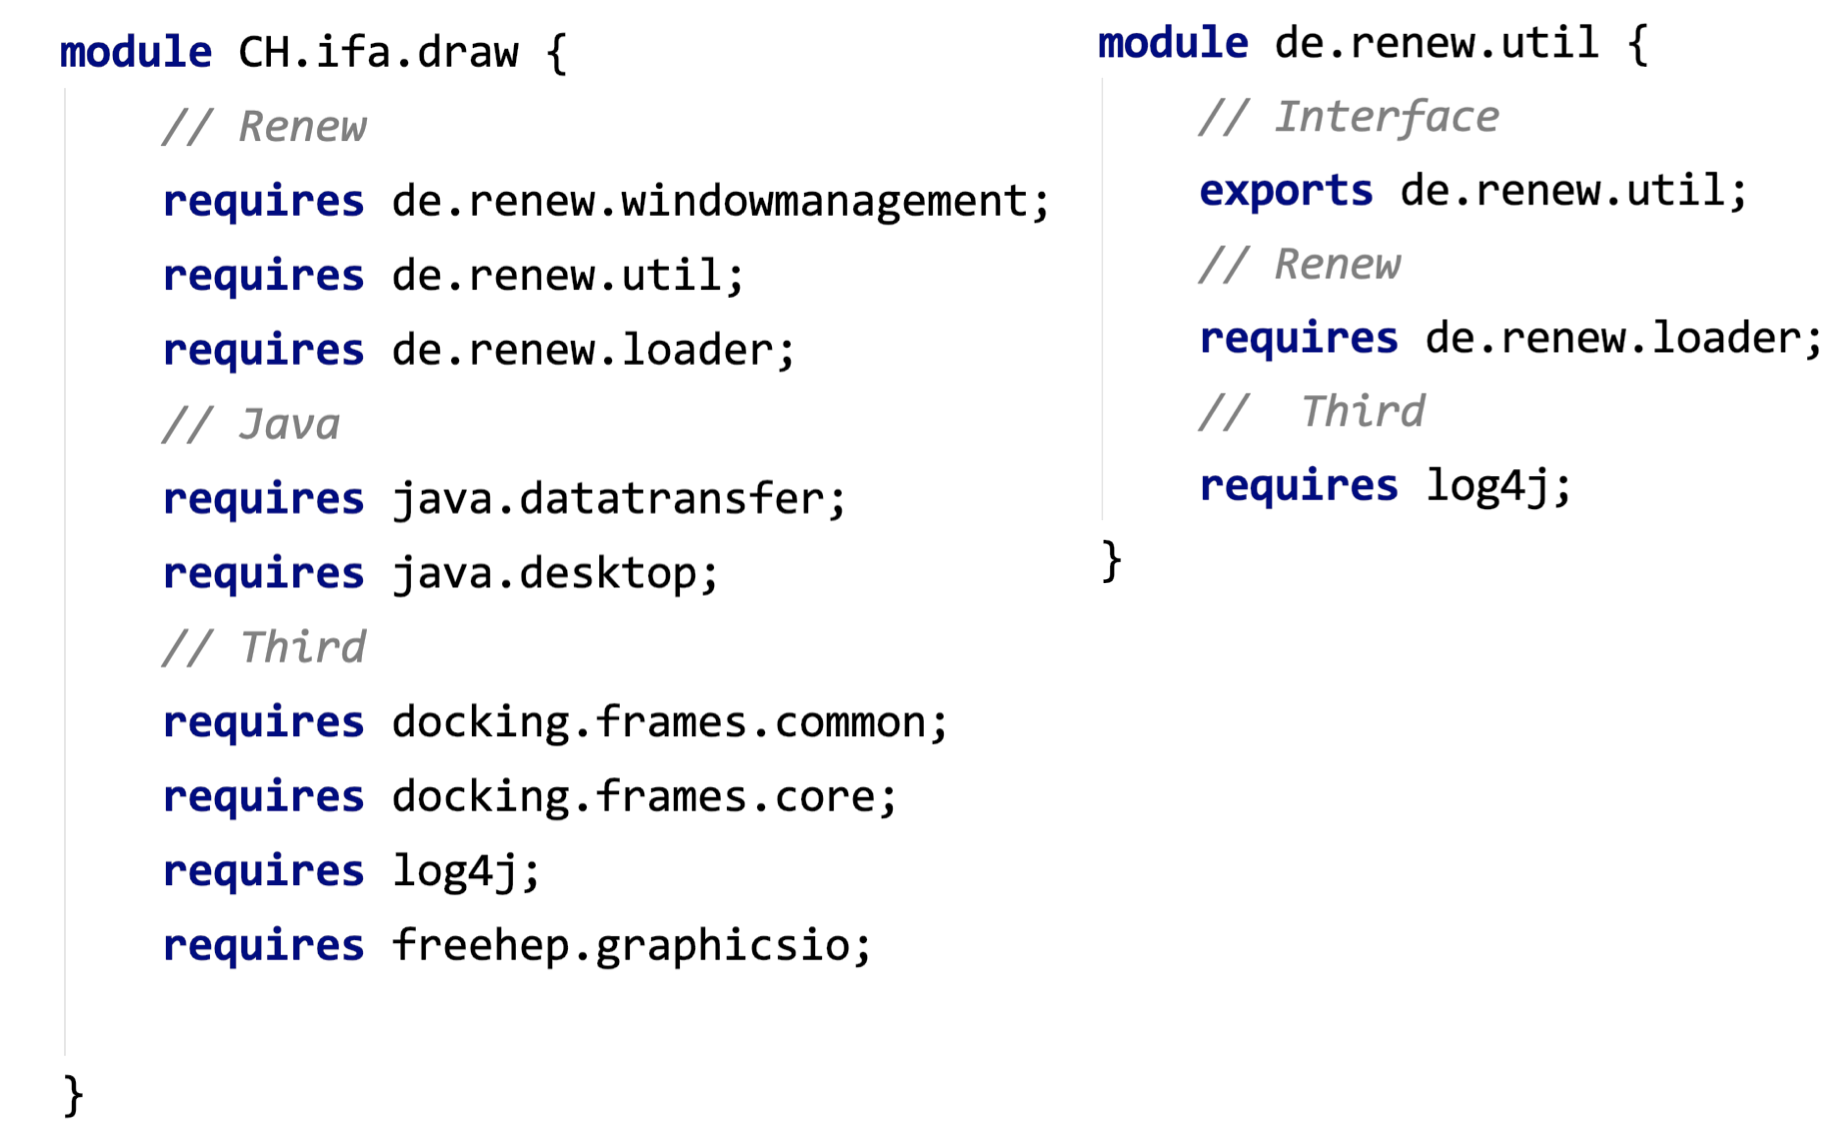
\includegraphics[width=0.7\textwidth]{material/images/utilCH-info.png}
	  \caption{Exportierte Pakete}
	  \label{fig:utilCH}
	\end{figure}

	In der Abbildung \ref{fig:utilCH} wurde das Util Plugin Modul angepasst und bietet jetzt das \textit{de.renew.util} Paket für den Gebrauch an.\newline
	Die Adaption der bestehenden Module muss mit jeder neuen Modulschicht an die angeforderten Pakete und Klassen angepasst werden, bis alle Abhängigkeiten erfüllt sind.\newline
	Damit sind die notwendigen Schritte für die Modularisierung bestimmt worden und können in einem Zyklus, bis alle Plugins auf dem Modulpfaden befinden, durchgeführt werden. Nähmilch das Auslesen und Definieren der Plugin Kompilation- sowie Laufzeit Abhängigkeiten aus dem Gradle Build Skript mit dem Schlüssel \textit{requires} und das Nachrüsten der Schnittstellen bestehender Module mit dem \textit{exports} Schlüssel. \bigbreak

	In der folgenden Abbildung wird die komplette Migration in vier Schritten dargestellt. Zuerst wird das \textit{Loader}, das \textit{Utils} und das \textit{Window Management} Plugin migriert, da diese laut der Ausgangssituation keine Abhängigkeiten im Klassenpfad besitzen und aus den Modulpfad auf den Klassenpfad nicht zugreifen müssen. Im nächsten Schritt werden Plugins modularisiert, die nur auf den Modulpfad Angewiesen sind. Das wären der \textit{Simulator} sowie \textit{JHotDraw} Plugin. Da alle Abhängigkeiten des \textit{Formalism} und \textit{Remote} Plugins auf den Modulpfad bewegt worden sind, können diese der Modulmenge beigefügt werden. Zum Schluss bleiben Plugins mit weit gefächerten Plugin Abhängigkeiten, wie zum Beispiel das \textit{Misc} oder das \textit{Gui} Plugin.  \bigbreak

	\begin{figure}[h!] 
	  \centering
	  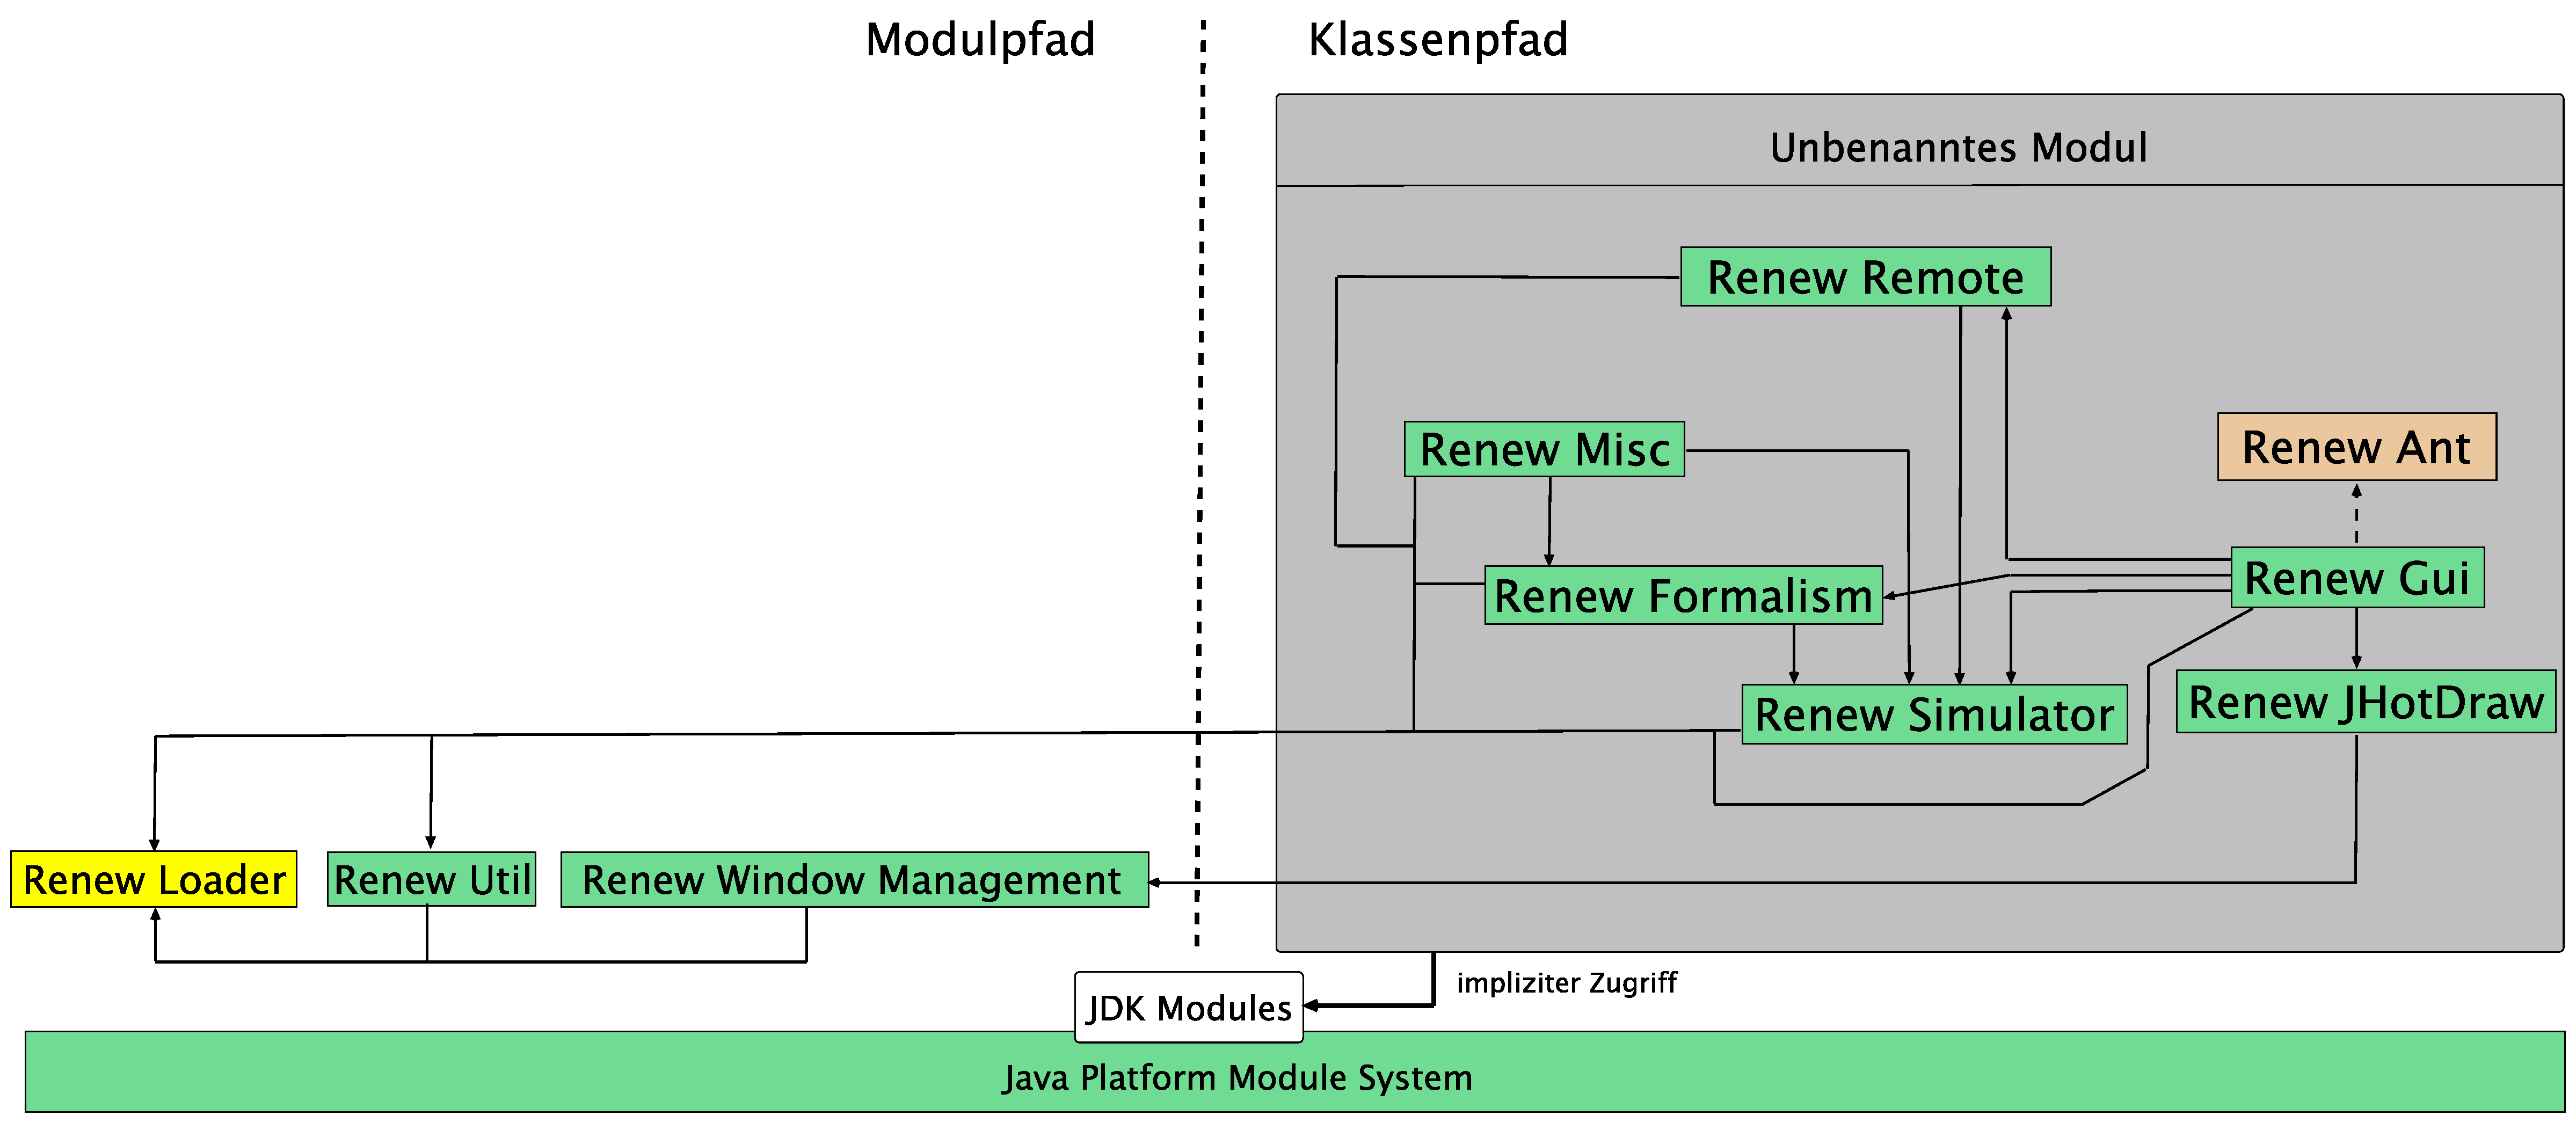
\includegraphics[width=0.997\textwidth]{material/images/renew_plugin_dependencies-migrate_1b.pdf}
	 \end{figure}
	\begin{figure}[h!] 
	  \centering
	  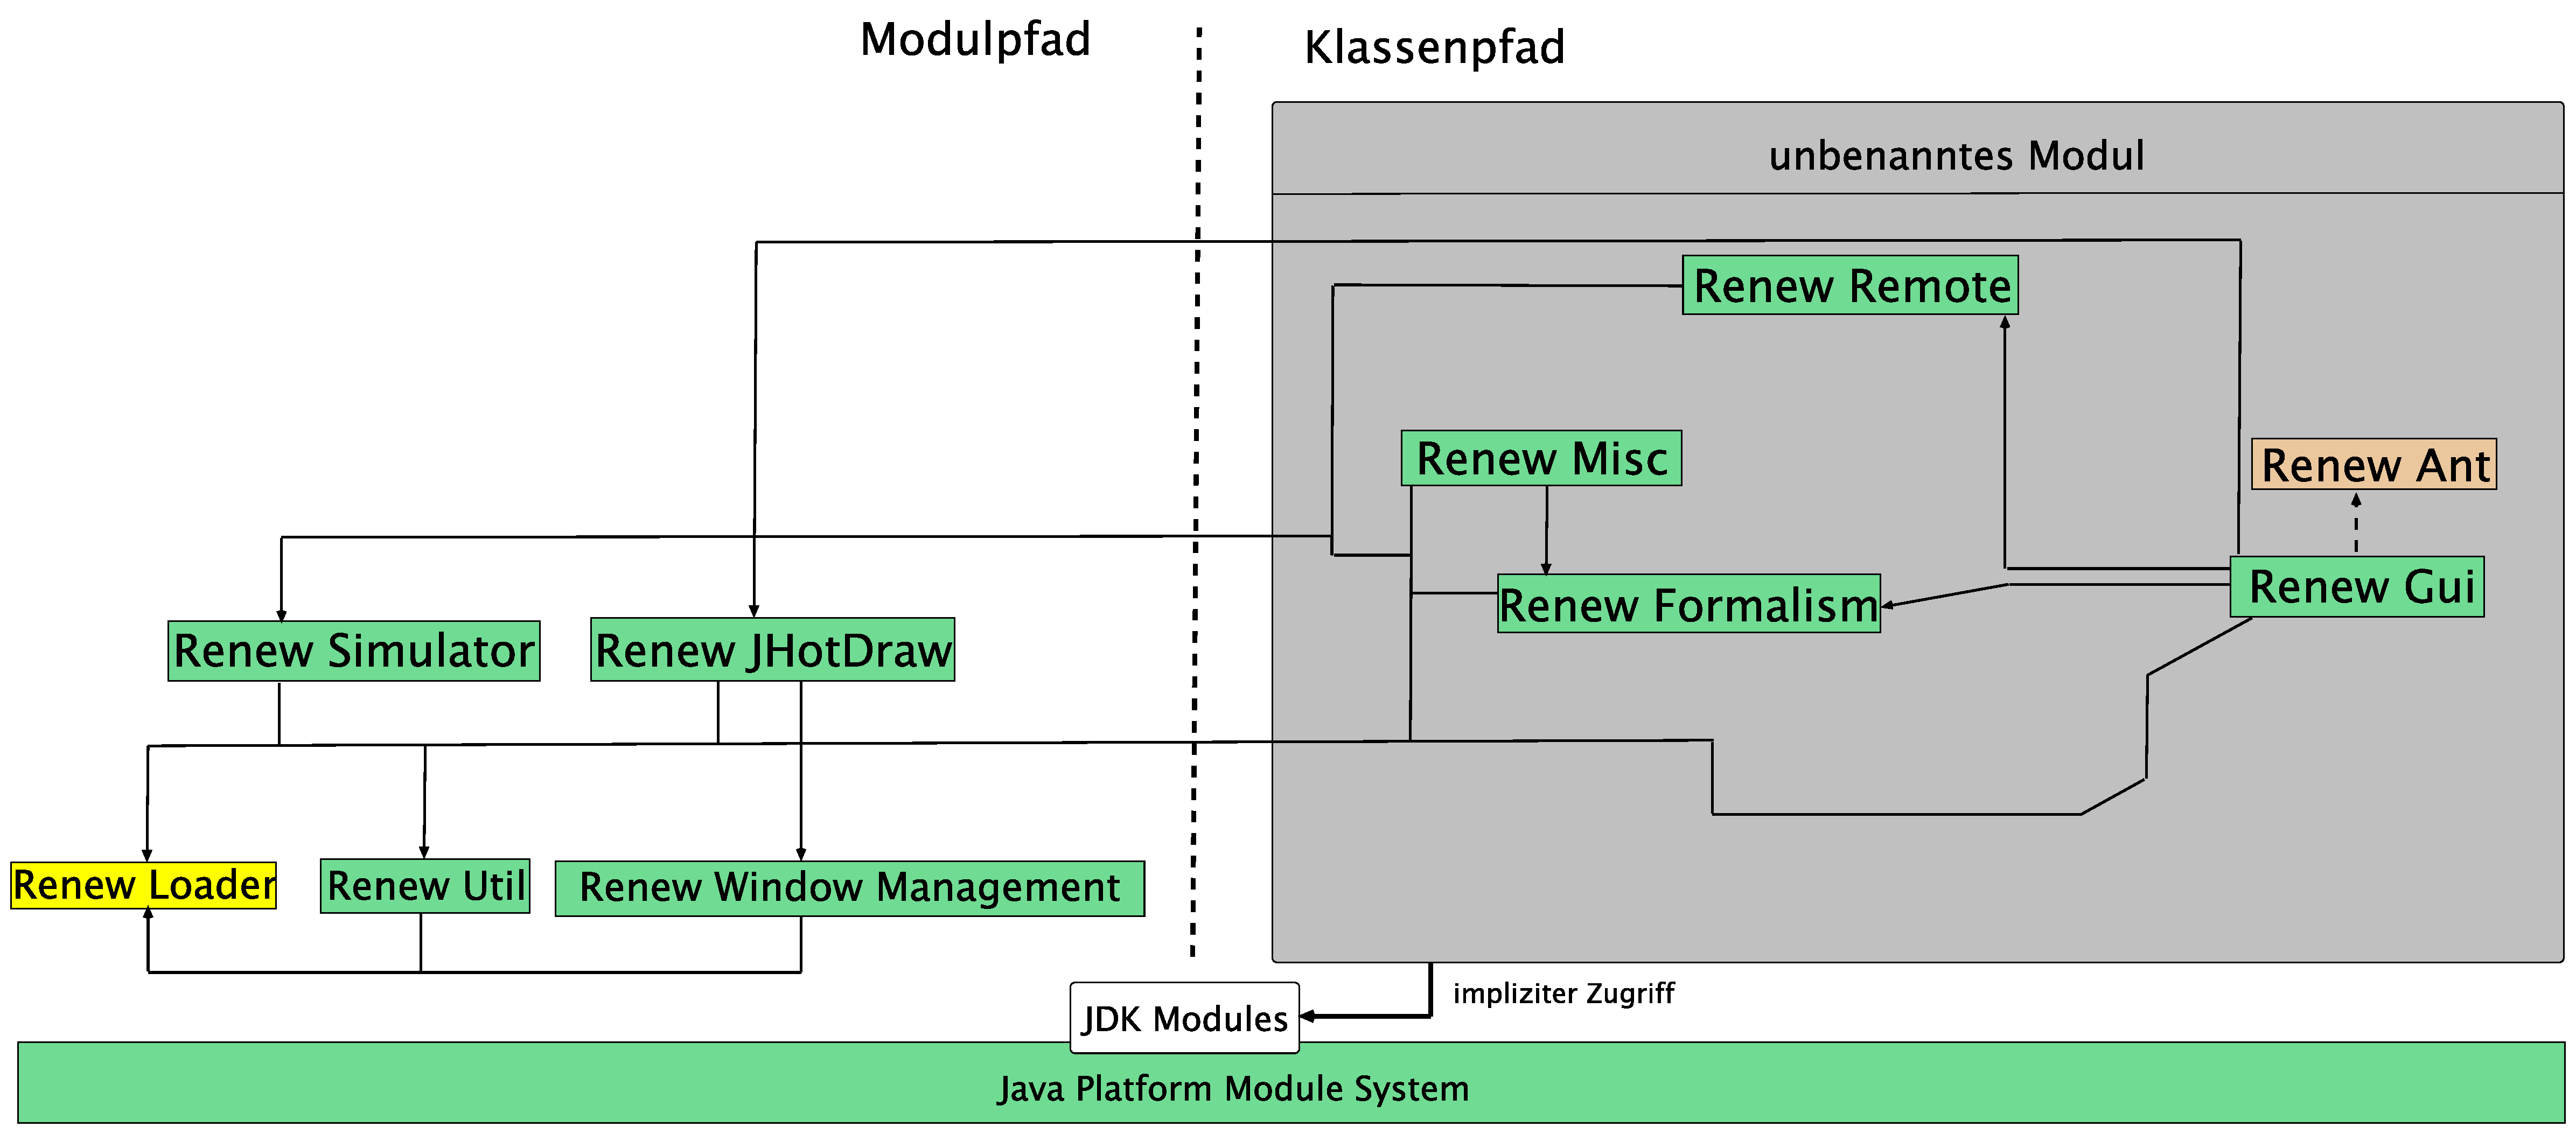
\includegraphics[width=0.997\textwidth]{material/images/renew_plugin_dependencies-migrate_2b.pdf}
	  \end{figure}
	 \begin{figure}[h!] 
	  \centering
  	  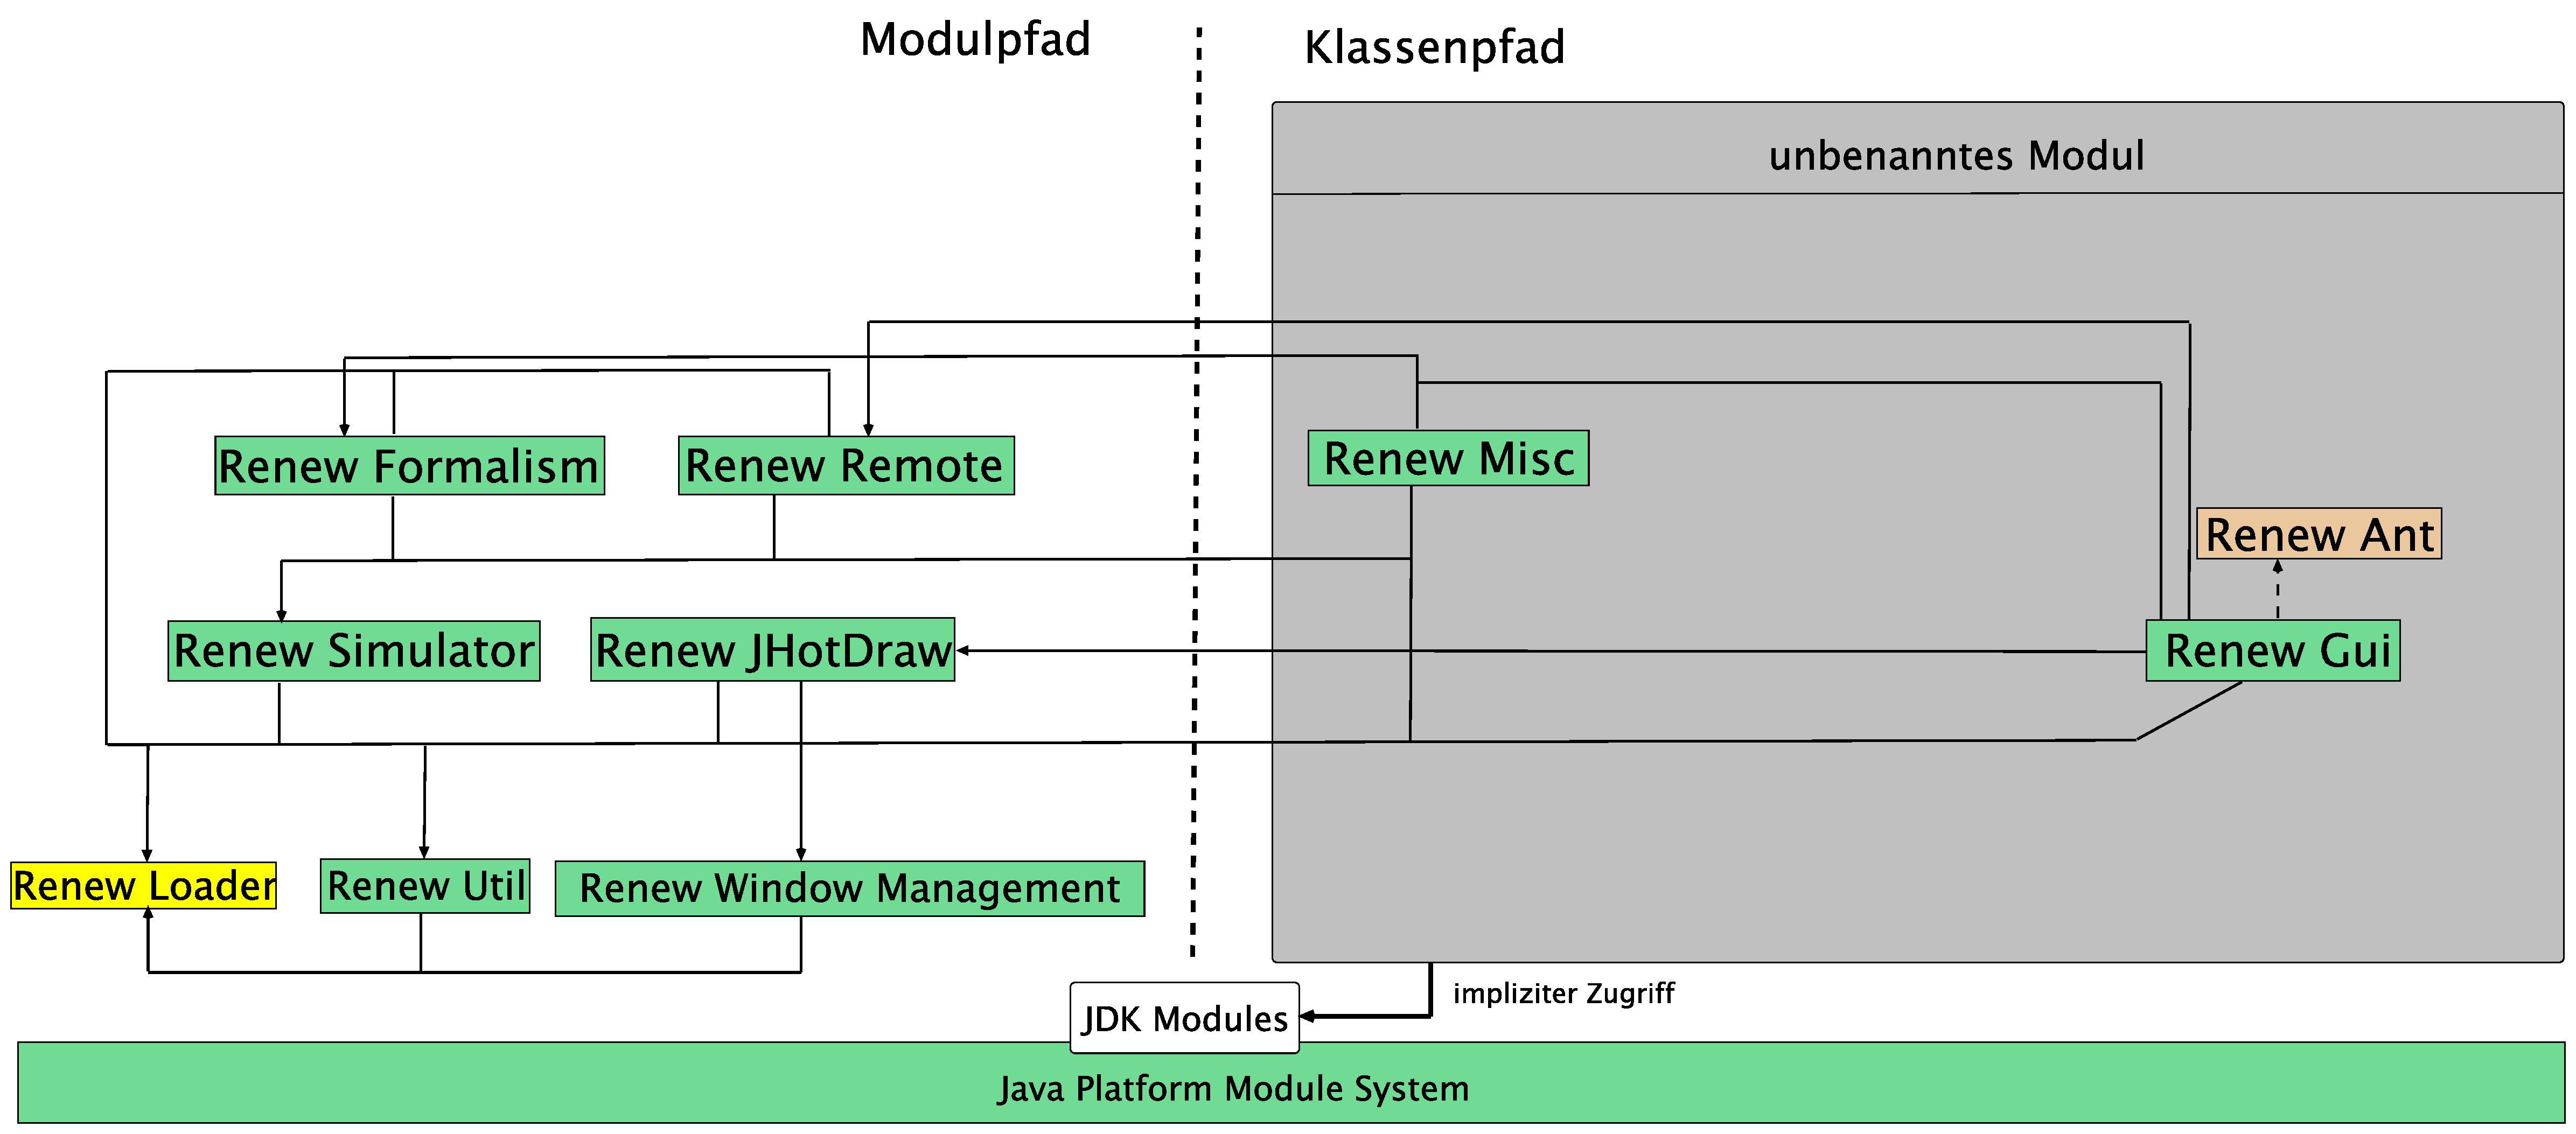
\includegraphics[width=0.997\textwidth]{material/images/renew_plugin_dependencies-migrate_3b.pdf}
  	  \end{figure}
  	 \begin{figure}[h!] 
	  \centering
  	  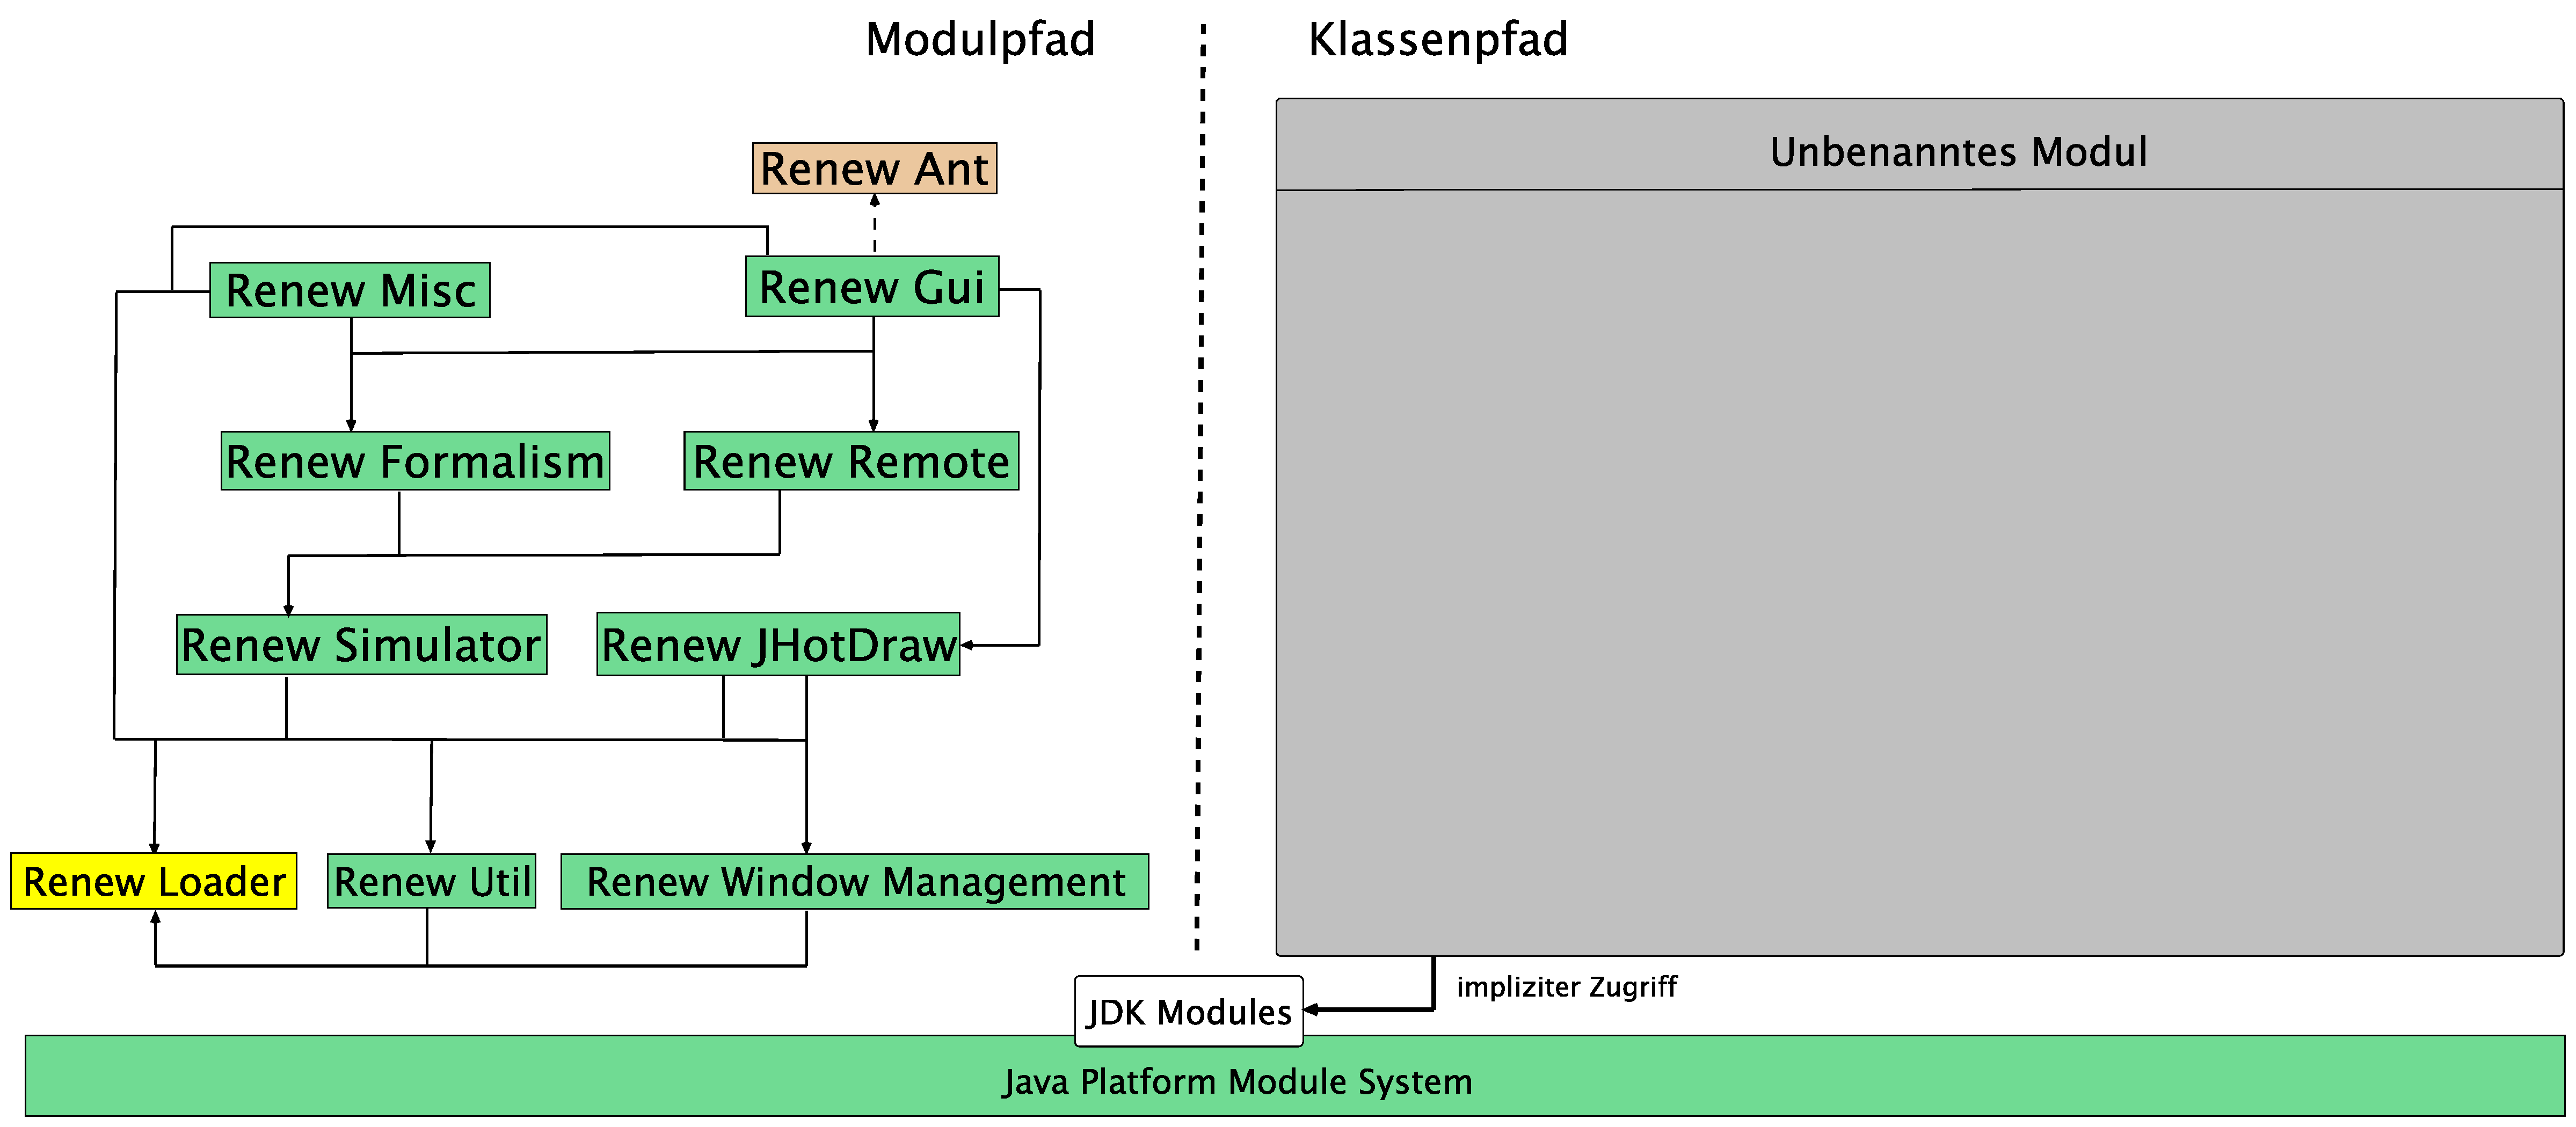
\includegraphics[width=0.997\textwidth]{material/images/renew_plugin_dependencies-migrate_4b.pdf}
  	  \caption{Migration}
	  \label{fig:mig}
	\end{figure}

\newpage
\section{Evaluation}
	Die Evaluation des ersten Prototyps bewertet das Ergebnis des gesetzten Ziels, nämlich die Erstellung einer minimalen \textsc{Renew} Version für das Modulsystem von Java. Dafür werden die Schlüsselaktionen der Migration wie Projektstruktur, Projektverwaltung und die Modulumsetzung nacheinander kritisch beleuchtet.

\subsection{Struktur} \label{sub:struktur}
	Die Anforderung einer minimalen Version von \textsc{Renew} zu modularisieren und mit einem modernen Werkzeug zu verwalten wurde erfüllt. Diese Aufgabe beinhaltete das Umstrukturieren der Plugin Code Basis, die es erlaubt zusätzliche Module innerhalb eines Plugins anzulegen. Jedoch gab es unerwartete Strukturänderungen, die durchgeführt werden müssen. Zum Beispiel besitzen einige Plugins wie das Util, Loader und Simulator Plugin Test Klassen, die in die neue Struktur eingebunden werden müssen. Demzufolge musste laut dem Maven Standard Layout ein \textit{src/test/java/module.name} Test Ressourcen, mit den dazugehörigen Test Klassen, angelegt und verwaltet werden. \newline

	Des Weiteren werden JavaCC Klassen separat von den Java Ressourcen untergebracht und von einem Gradle Plugin ausgeführt. Dies hat zu Folge, dass der generierte Code umgeleitet werden muss, um an der entsprächen Position die Funktion zu erfüllen. Zusätzlich muss JavaCC den Java Code generieren, bevor der Java Compiler mit der Übersetzung beginnt, denn die generieren Java Klassen bilden die Basis für die Plugins und somit sind sie zwingen erforderlich für die Kompilation. Dies bezüglich wurde der \textit{Gradle Task Graph} modifiziert, um die entsprechende Reihenfolge zu erfüllen. Daraus ergibt sich Komplexität, die neu für \textsc{Renew} ist und in der Zukunft sorgfältig gewartet werden muss. \bigbreak

\subsection{Verwaltung} \label{sub:verwaltung}
	Ein wesentlicher Vorteil der modernen \textit{build} Tools wie Gradle und Maven, ist die Verwaltung der verwendeten Drittanbieter-Bibliotheken. Diese laden und binden benötigte Bibliotheken mit dem kompletten Abhängigkeitsgraphen in das Projekt ein, ohne den Zwang der Einarbeitung des Entwicklers in die Struktur der genutzten Bibliothek. Somit wird viel Zeit gespart, da man sich mit dem Kontext und der darunter liegenden Bausteinen, wie Core, Common und Util, der genutzten Bibliotheken nicht beschäftigen muss. \newline

	Die Verwaltung der Bibliotheken spielt eine große Rolle für Renew, da im Verlauf der Entwicklung, Drittanbieter-Bibliotheken angepasst wurden und somit keine Möglichkeit besteht eine saubere Version der Bibliothek einzubinden. Infolgedessen entstehen  unsaubere Abhängigkeiten, die nicht aktualisiert werden können. Diese werden wie zuvor, durch das Auslesen aus einem lokalen \textit{libs} Verzeichnis, in das Projekt eingebunden und müssen in der Zukunft, für die saubere Umsetzung von der benutzerdefinierten Logik befreit werden.\bigbreak

	Ein zusätzlicher Vorteil der neuen Projektverwaltung liegt an der neuen Umsetzung mit einer Programmiersprache, die es erlaubt mit Felder, Variablen, Schleifen und Objekten zu arbeiten. Dies hat zu Folge, dass der Übergang von den \textsc{Renew} Java Code zu den \textit{build} Skript von Gradle für den Entwickler leichter nachzuvollziehen ist und somit Akzeptanz und Anpassungsfähigkeit mit sich bringt. \newline
	Hierzu kann die Verständlichkeit des Gradle Werkzeug gegenüber dem Ant Werkzeug an der benötigten Code Menge, die geschrieben werden muss, abgelesen werden. Zum Beispiel benötigt die Ant Version von Renew, die zurzeit alle Plugins und den kompletten Umfang der Applikation verpackt, um die 740 Zeilen für die globale Konfiguration und 135 Zeilen für jedes Projekt. Im Gegensatz dazu wiegt die minimale Gradle Version von \textsc{Renew} 136 Zeilen für die globale Konfiguration und nur 20 Zeilen für jedes Plugin im Durchschnitt. Zusätzlich ist die Konfiguration von simplen Plugins mit vier Zeilen möglich und kann von jedem Entwickler erstellt und angepasst werden.

	\begin{figure}[h!]
	  \centering
	  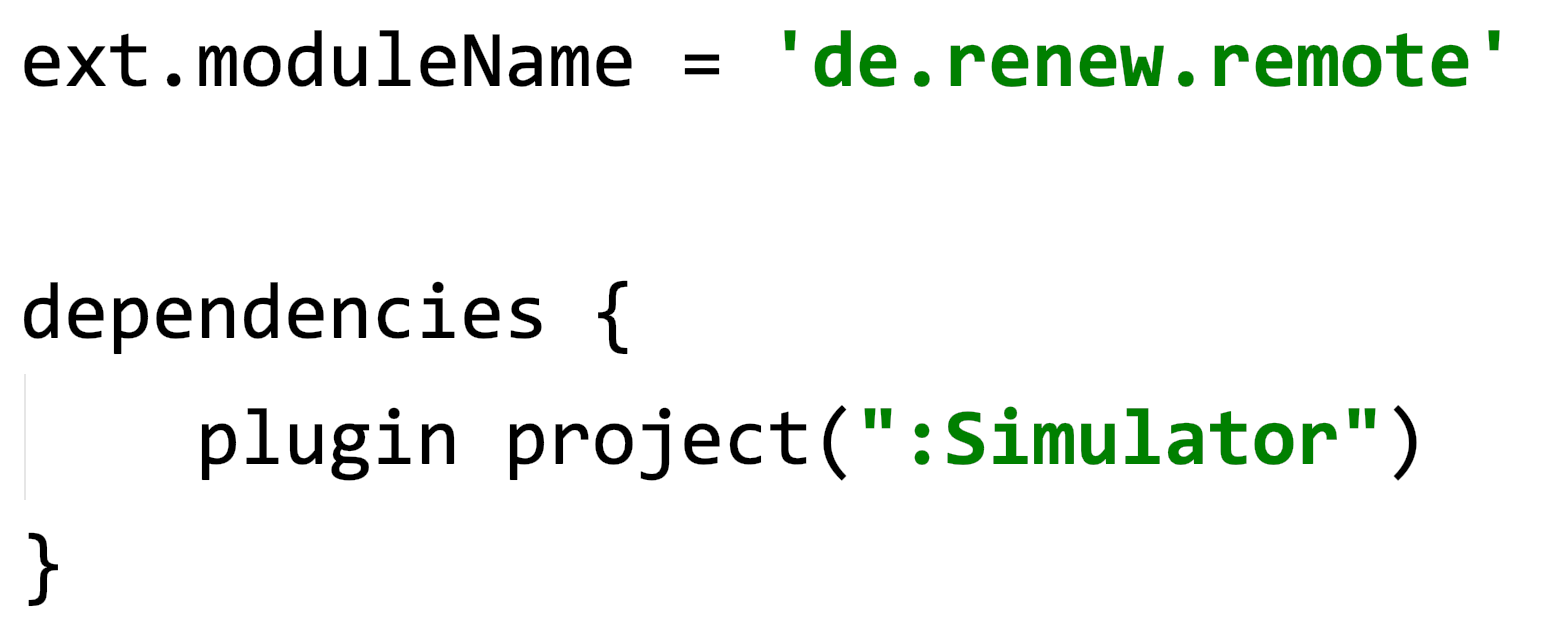
\includegraphics[width=0.5\textwidth]{material/images/Remote_config.png}
	  \caption{Remote Plugin Konfiguration}
	  \label{fig:remote_config}
	\end{figure}	

	Obwohl die globale Konfiguration für die vollständige \textsc{Renew} Version sich steigern wird, deuten die Zahlen auf einen geringeren Code-Abdruck des Gradle \textit{build} Werkzeugs hin.\bigbreak

\subsection{Modulumsetzung} \label{sub:optimierung}% aufwertung
	Nachdem die Modularisierung abgeschlossen wurde, ist eine globale Sicht auf die Umsetzung möglich und offenbart Optimierungspotenzial für die Abstimmung der Modulabhängigkeiten. Zum Beispiel wird das RenewAnt Plugin nur für die Kompilation benötigt und muss nicht für die Ausführung mitgeliefert werden \ref{fig:remote_config}. Daher kann dieses als eine statische Abhängigkeit im Gui Plugin verankert werden und wird der Laufzeit nicht beigefügt.\bigbreak

	\begin{figure}[h!]
	  \centering
	  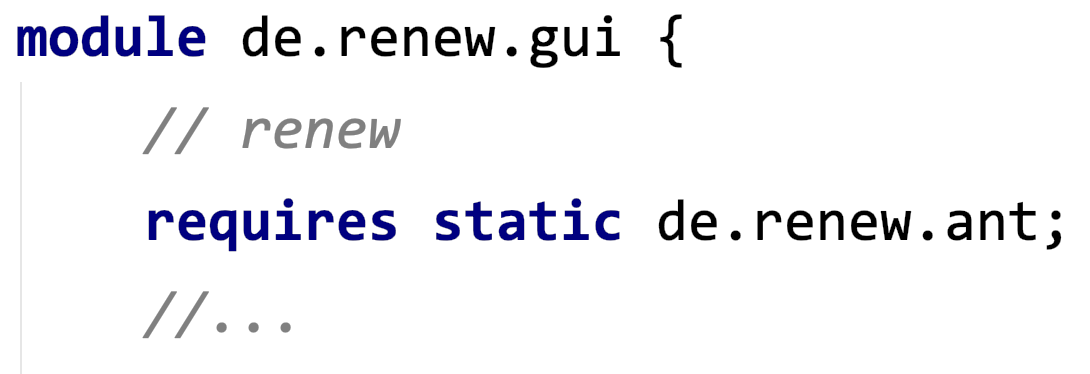
\includegraphics[width=0.4\textwidth]{material/images/gui_config.png}
	  \caption{Statische Konfiguration}
	  \label{fig:remote_config}
	\end{figure}

	Des Weiteren wird klar, dass die \textsc{Renew} Applikation in einer hierarchischen Plugin Architektur aufgebaut ist. Das heißt Plugins, die von anderen Plugins abhängig sind, erfordern das Einbinden aller darunter liegenden Schichten. Dies hat zur Folge, dass das \textit{Util} Plugin in jedem Plugin, das auf diesen und seinen Nachfolger aufbaut, eine Deklaration benötigt. \newline

	Um die Übersicht über die unmittelbar genutzten Module zu behalten, kann mithilfe des \textit{transitiv}  Schlüssels eine angeforderte Bibliothek für alle Nutzer-Plugins offengelegt werden. Demzufolge kann ein Plugin nicht nur ein anderes Plugin erweitern und nutzen, sondern seinen Kontext in die Umsetzung miteinbeziehen. \bigbreak

	\begin{figure}[h!]
	  \centering
	  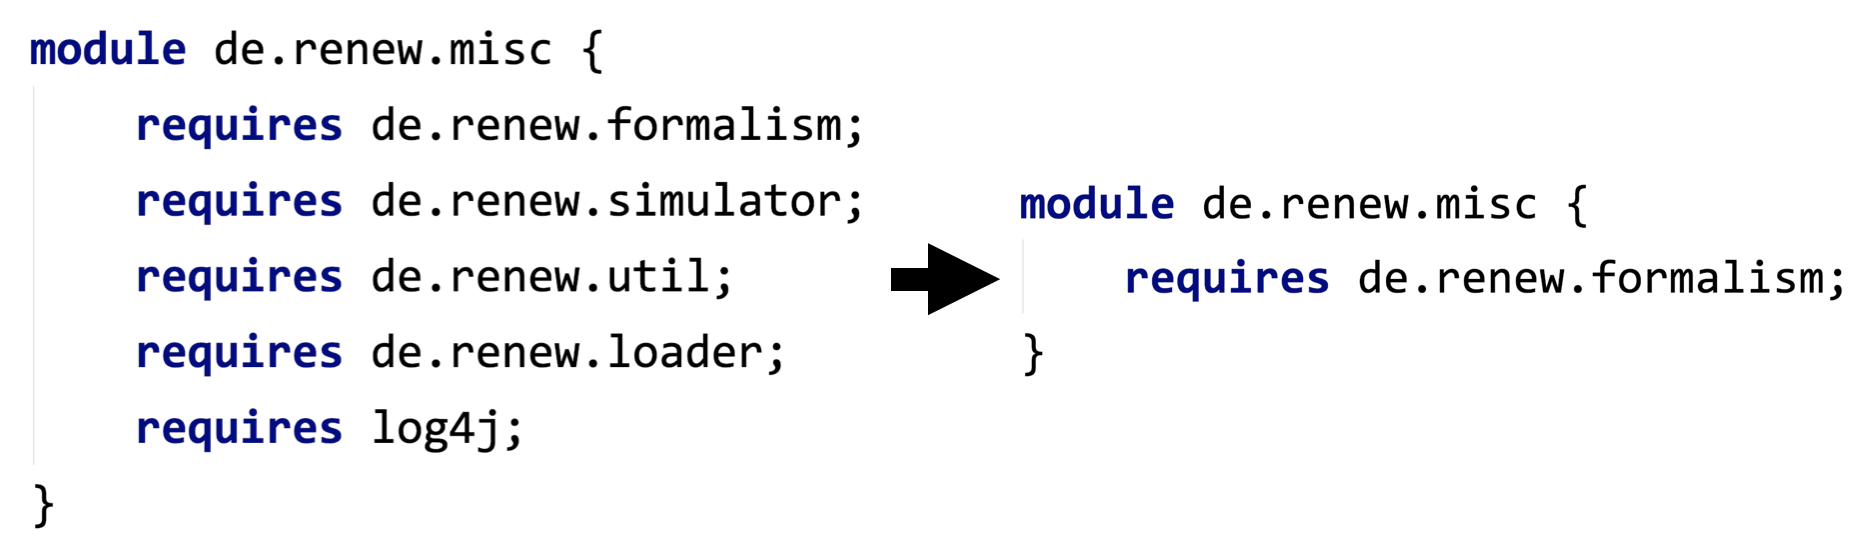
\includegraphics[width=0.8\textwidth]{material/images/misc_trans.png}
	  \caption{Transitive Konfiguration}
	  \label{fig:trans_config}
	\end{figure}

	Um den aktualisierten Java Kontext so gut wie möglich nachzubilden, unterstützt Gradle die Idee der  Modularisierung und dessen Kopplungsarten, indem die Modulkopplung unter Verwendung von unterstützenden API's zum Entwerfen der transitiven und statischen Abhängigkeiten angeboten wird. Diese bestehen aus zwei weiteren Konfigurationspfaden, die durch \textit{api} und \textit{implimentation} gekennzeichnet sind. Die \textit{api} Konfiguration beschreibt eine transitive Abhängigkeit, die durch die Modulhierarchie weitergereicht wird und die \textit{implimentation} Konfiguration, die die genutzten Bibliotheken privat nutzt. Somit können die transitiven \textsc{Renew} Abhängigkeiten, die in der \textit{module-info.java} deklariert sind, auf die Projektstruktur mithilfe von Gradle abgebildet werden.

	\begin{figure}[h!]
	  \centering
	  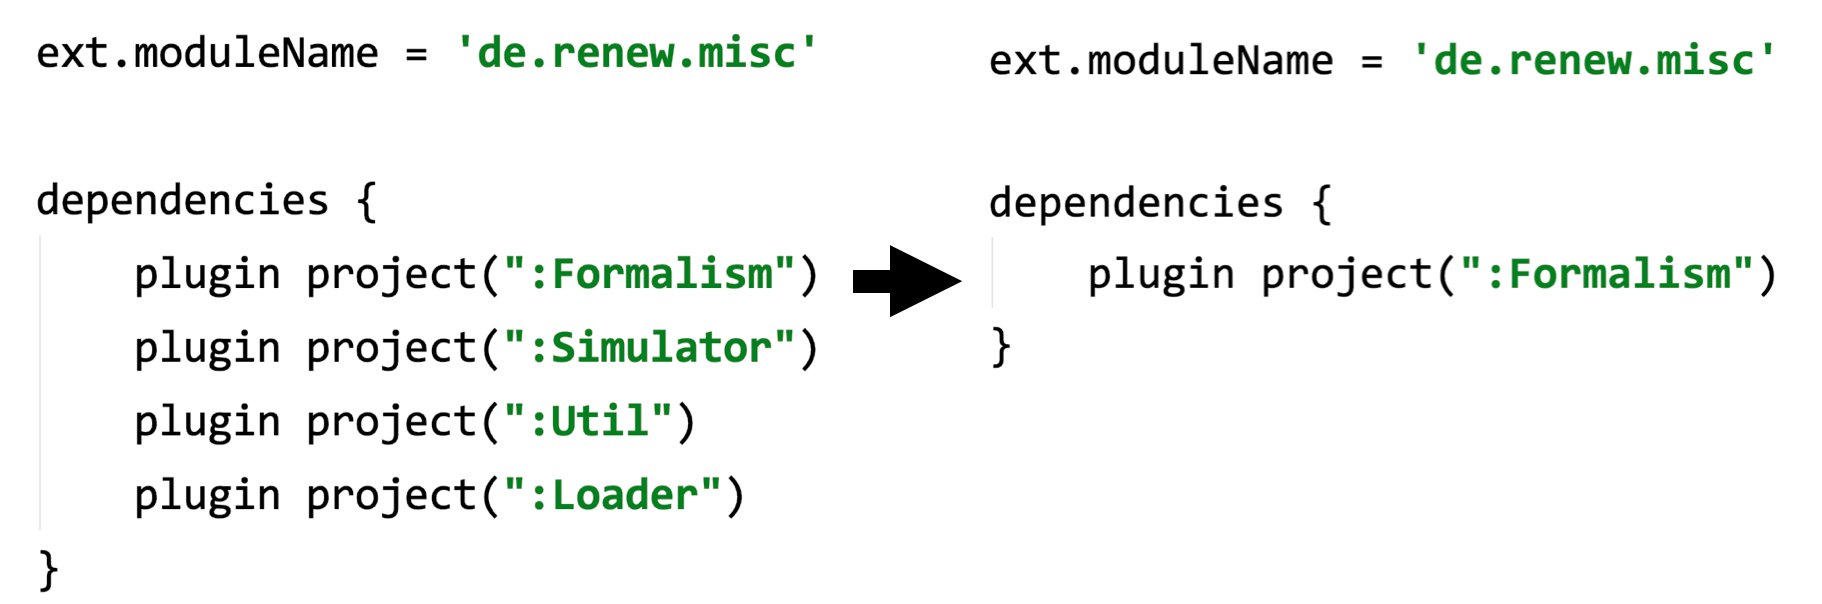
\includegraphics[width=0.8\textwidth]{material/images/gradle_misc.png}
	  \caption{Transitive Gradle Konfiguration}
	  \label{fig:trans_gradle}
	\end{figure}

\subsection{Endergebnis} \label{sub:endergebnis}
	Nachdem \textsc{Renew} verfeinert wurde, entsteht eine eindeutige Darstellung der Plugin Abhängigkeiten und dessen Aufbau. Ersichtlich wird, dass Module eine einfache Art und Wiese bieten, um den Aufbau komplexer Systeme zu Verwalten und Umstrukturieren.

	\begin{figure}[h!]
	  \centering
	  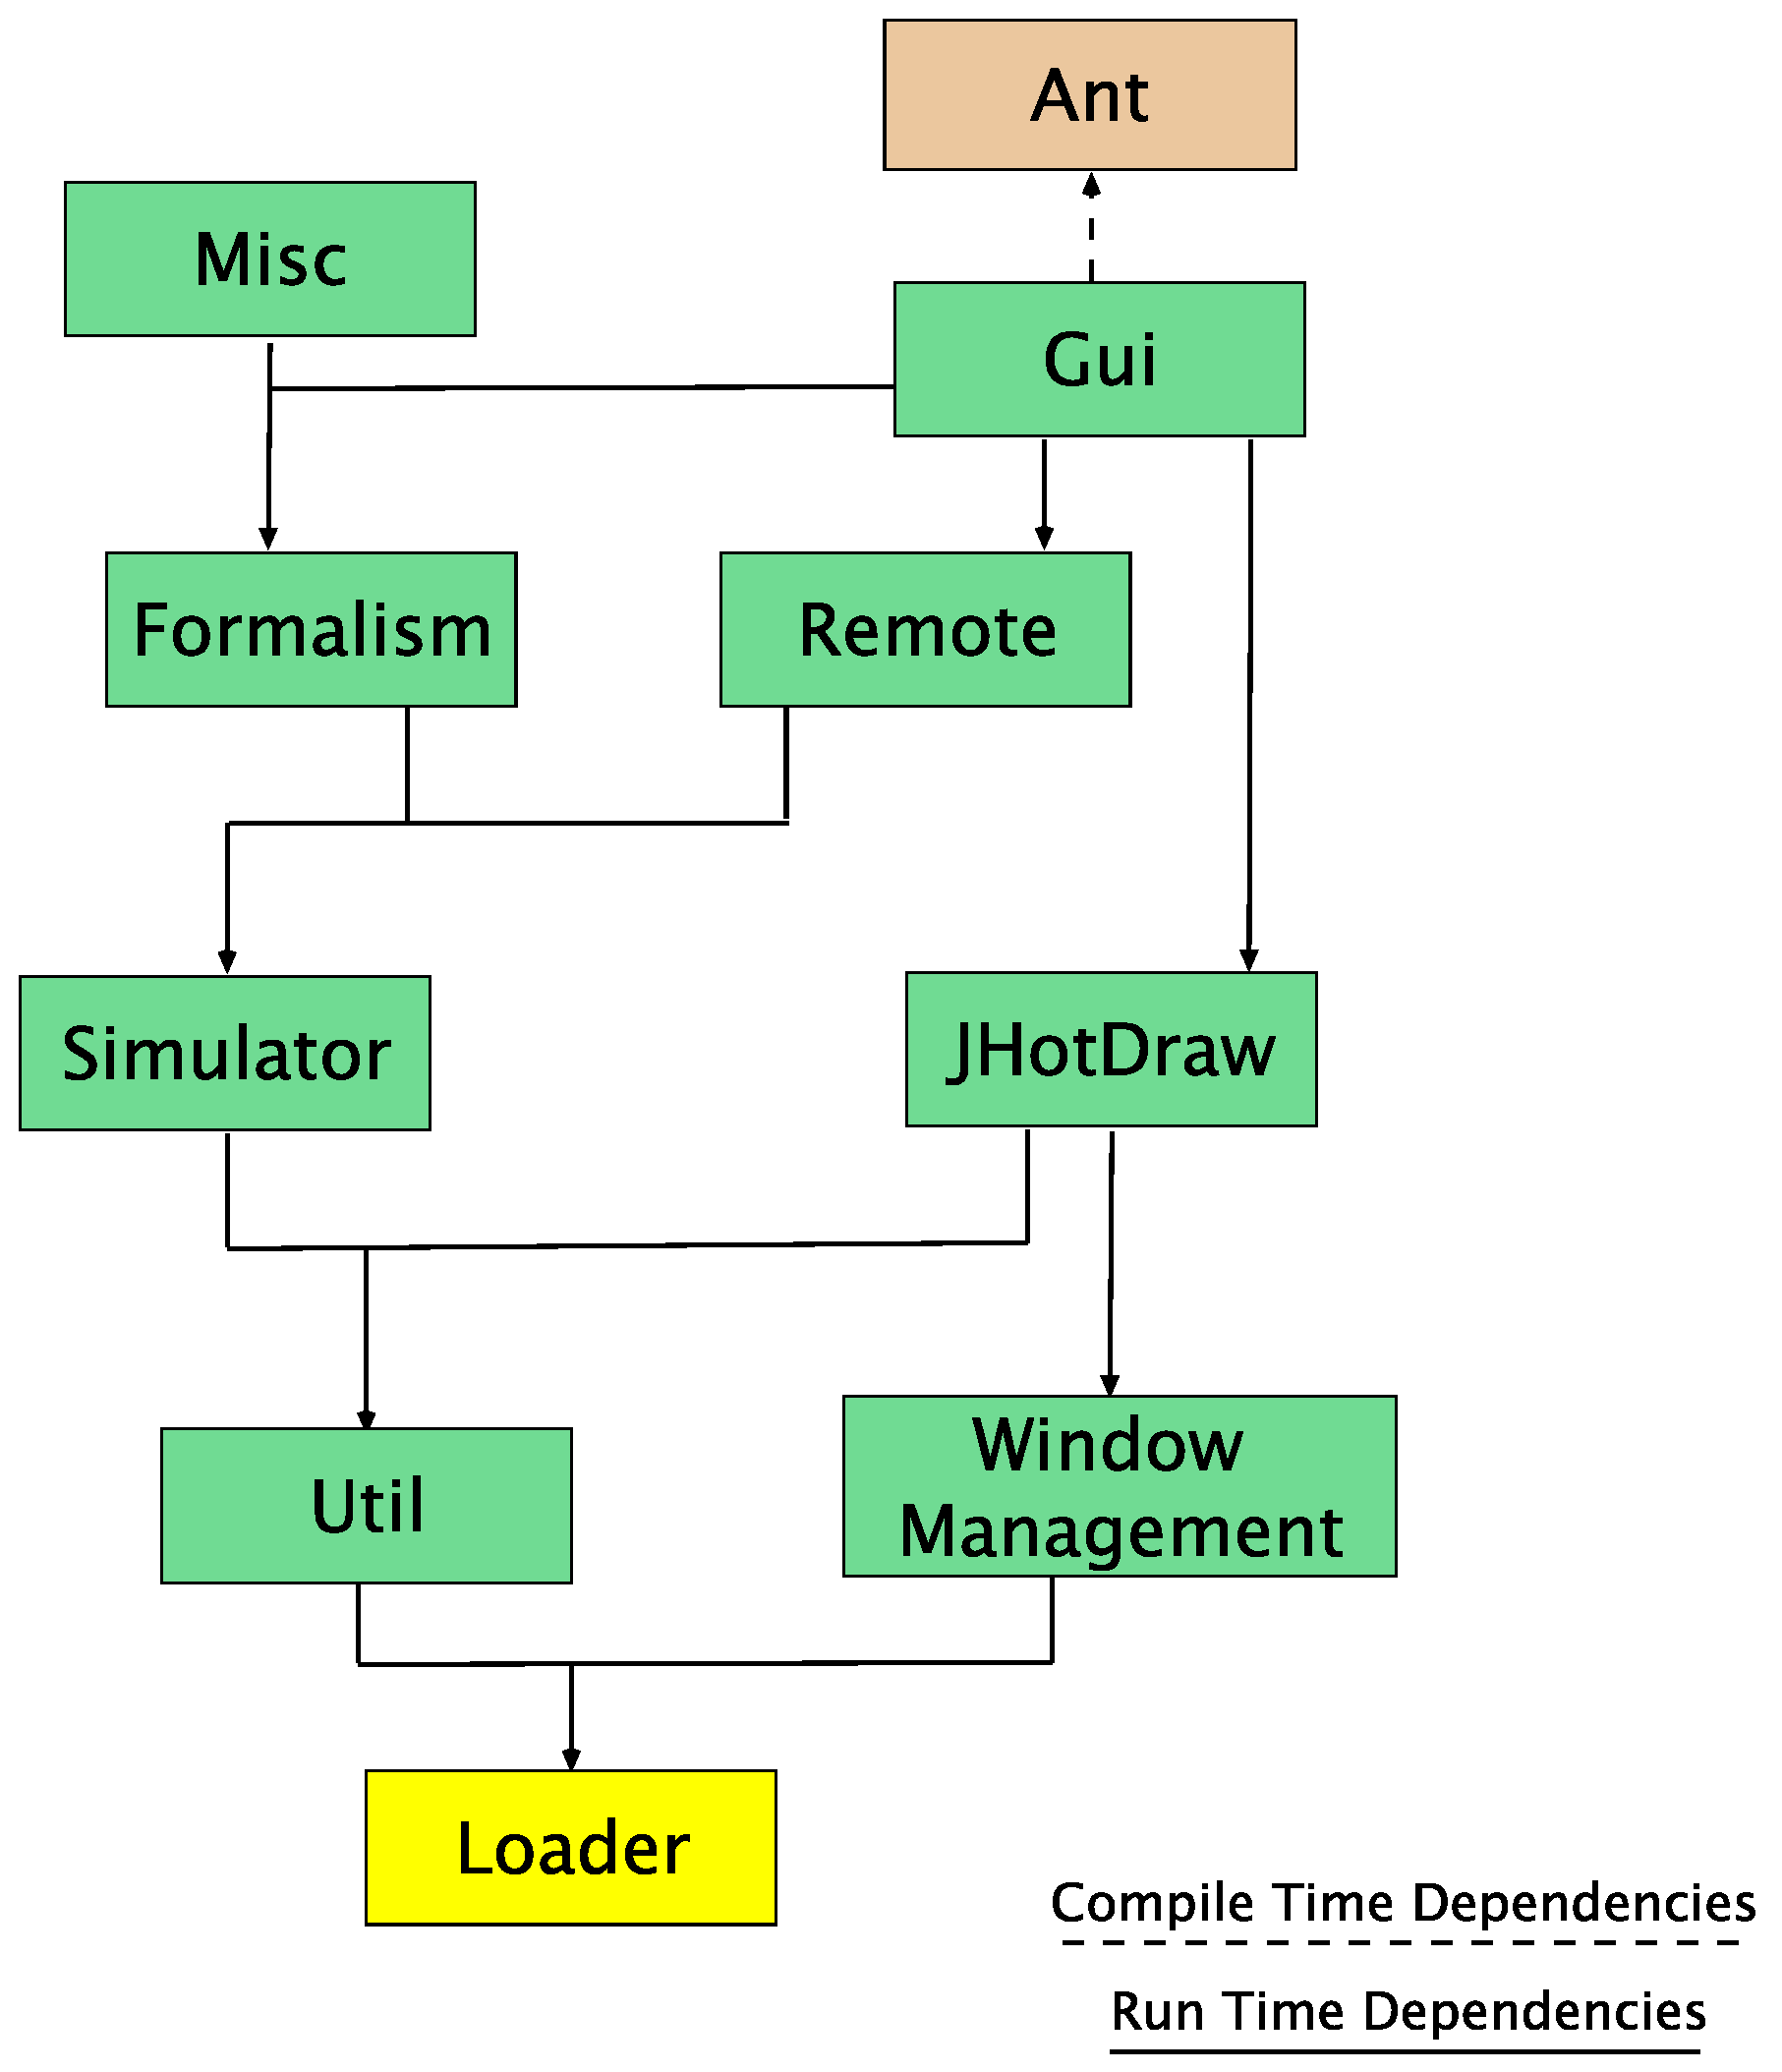
\includegraphics[width=0.8\textwidth]{material/images/renew_plugin_dependencies-migrate_opt.pdf}
	  \caption{Minimale modulare \textsc{Renew} Version}
	  \label{fig:trans_config}
	\end{figure}
% Kritik: Module brauchen explezite schnittstellen, in unseren Fall wurde lediglich die benötigte Logik für die nutzung geöffnet.
% Gradle: Trennen der Klassenpfade hilft die Struktur zu verwalten automatic, plugin, runtime, compile, api und implimentation. 
 
\chapter{Mulan Prototyp} \label{cha:mulan_settler}
	Die Siedler oder Settler ist eine Aufbau-Strategiespiele, das unter Verwendung der Mulan (Multi-Agent Nets) Plattform aufgebaut und mit Renew simuliert werden kann. \bigbreak
	Für die Gestaltung der Mulan-Settler Variation wird zunächst der Aufbau der Gesamtumsetzung geschildert und der Zusammenhang der Akteure dargestellt. Anschließend werden Anforderungen erfasst, die der Renew Prototyp erfüllen muss, um die Mulan-Settler Variation der Mulan Plattform zu betreiben. Infolgedessen entsteht ein Implementierungsplan sowie ein Prototyp.

\section{Anforderungen} \label{sec:anforderungen2}
	Der Mulan-Settler Renew Prototyp soll die Mulan Plattform unterstützen, dabei sind nur die für Settler nötigen Mulan-Plugins einzubringen, die auf dem modularen Renew ihre Funktion erfüllen sollen. Das Ergebnis soll eine UI präsentieren und geringe Interaktionsmöglichkeiten anbieten. \newline 
	Ziel des Prototypen ist die Darstellung des parallelen Betriebs von alten und neuen Softwarekomponenten, die mithilfe des Modulsystem von Java zusammengeführt werden können und in der Konsequent als ein Beispiel für eine Migration ohne  Zeitdruck und Betriebsausfall dienen.

\section{Spezifikation}
	Für die Umsetzung des Prototyps muss die minimale Renew Version neu definiert werden, denn die Mulan Plattform im Kontext des Settler Plugins benötigt eine größere Menge an Renew Plugins. Dafür müssen die erforderliche Mulan Plugins für Settler ausgelesen werden, um anschließend die entsprechenden Renew Abhängigkeiten abzuleiten. \newline
	Da die Mulan Plugins auf die Renew-Codebasis angewiesen sind und dessen Klassen für das Kompilieren, Bauen und das Ausführen der Plugins benötigen, müssen die entsprechenden Referenzen in den Mulan Plugins, Ressourcen und \textit{Ant} Skripten angepasst werden. \newline
	Die Settler und Mulan \textit{Ant} Skripte sollen nicht auf das \textit{Gradle} Werkzeug migriert werden, statt dessen werden lediglich Anpassungen an die neue Renew Struktur durchgeführt. \bigbreak
	Die Basis für diesen Prototypen sollen alle Renew sowie Mulan Plugins aus den Abhängigkeitsgraph des Settler Spiels bilden, die aus der \textit{plugin.cfg} Konfigurationsdatei für die Laufzeitumgebung und aus dem \textit{Ant} Skript für die Kompilierumgebung abgelesen werden können. 


\section{Entwurf}
	Zuerst werden Komponenten in Form der benötigten Plugins aus Renew und Mulan für das Settler Spiel erarbeitet und der Zusammenhang zwischen den Applikationen abgebildet.\bigbreak
	Nachdem die Basis für das Settler Spiel erarbeitet wurde, müssen die \textit{Ant Skripte} an das modulare Renew angepasst werden, damit diese die passenden Renew Klassen für das Kompilieren interner Mulan Strukturen genutzt werden können. Zum Teil werden es interne Plugin Klassen sein und zum Teil werden kritische Ressourcen, wie \textit{Shadow Netze}, mithilfe der Renew Basis übersetzt. Daher ist das nahtlose Verzahnen zwischen Mulan und dem modularen Renew Prototypen das Schlüsselkriterium der Umsetzung. \bigbreak
	Da das modulare Renew auf der Abschlussarbeit von Martin Wincierz \cite{martinWinc} aufbaut, ist Mulan für die Oberflächenanpassung zu diesem Zeitpunkt nicht bereit und muss nicht nur an das modulare Renew, sondern auch an die erweiterte Oberfläche von Renew angepasst werden.\newline
	Somit ist das Aufsetzen des Settler Spiels und der erforderlichen Mulan Plugins mit Schwierigkeiten verbunden die sorgfältig behandelt werden müssen. 

\section{Umsetzung}
	Zuerst wird die existierende Struktur von Mulan betrachtet und die Settler Abhängigkeit laut den \textit{plugin.cfg's} abgelesen. Dafür werden die Settler Abhängigkeit innerhalb Renew und Mulan betrachtet und ein Abhängigkeitsgraph erstellt. Da die Mulan Plugins auf Renew aufbauen, werden zusätzliche Plugins für die modulare Renew Umsetzung durch den Abhängigkeitsgraphen aufgedeckt. Wie zum Beispiel das Renew \textit{Feature Structure} Plugin, das an der Modellierung von Prozessen und der Erstellung von Ontologien beteiligt ist. \bigbreak

	\begin{figure}[h!]
	  \centering
	  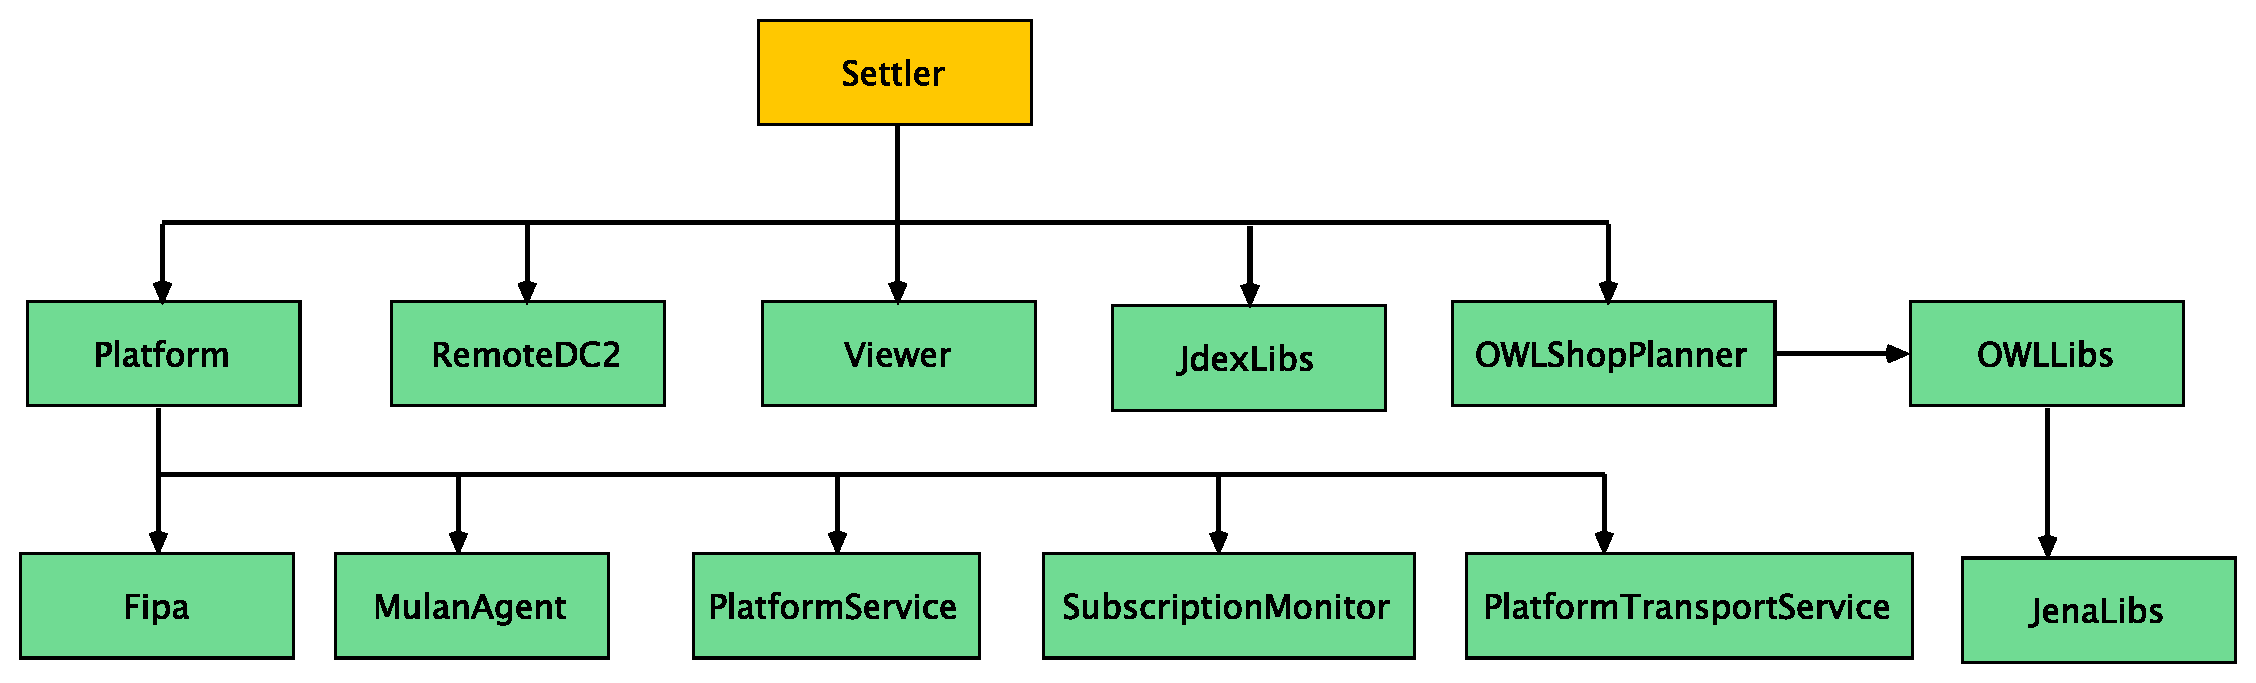
\includegraphics[width=\textwidth]{material/images/settler-mulan-plugins.pdf}
	  \caption{Settler Mulan Plugin Menge}
	  \label{fig:settler_mulan_plugins}
	\end{figure}

	Im Folgenden werden die benötigten Renew Plugins modularisiert und zum ersten Mal das Mulan Settler \textit{target} ausgeführt. Dieses soll das Settler Spiel mit allen nötigen Abhängigkeiten von Mulan sowie Renew kompilieren und verpacken. Jedoch wird man während der Ausführung auf Plugin Klassen verwiesen, die für das Kompilieren notwendig sind und nicht als Teil des Settler \textit{target's} sowie der \textit{plugin.cfg's} gelistet sind. \newline
	Die nachfolge Analyse ergab zusätzliche Abhängigkeiten aus den \textit{Plattform Transport Service} sowie \textit{Subscription Monitor} Plugins, die ein älteres Plugin ersetzen und noch nicht komplett in die Ant Umgebung eingebunden sind. Daher werden diese in den Settler Ant \textit{target} verankert sowie in den \textit{CAPA} Plugin \textit{plugin.cfg} nachgerüstet. In der Konsequenz muss der Abhängigkeitsbaum durch die nachträglichen Mulan Plugins erweitert und auf zusätzlicher Renew Plugins inspiziert werden. \newline
	In den Abbildungen \ref{fig:settler_mulan_plugins} sowie \ref{fig:renew_mulan_plugins} werden die endgültigen Plugin Mengen aus Mulan sowie Renew dargestellt, die Settler für die Ausführung benötigt. \bigbreak

	\begin{figure}[h!]
	  \centering
	  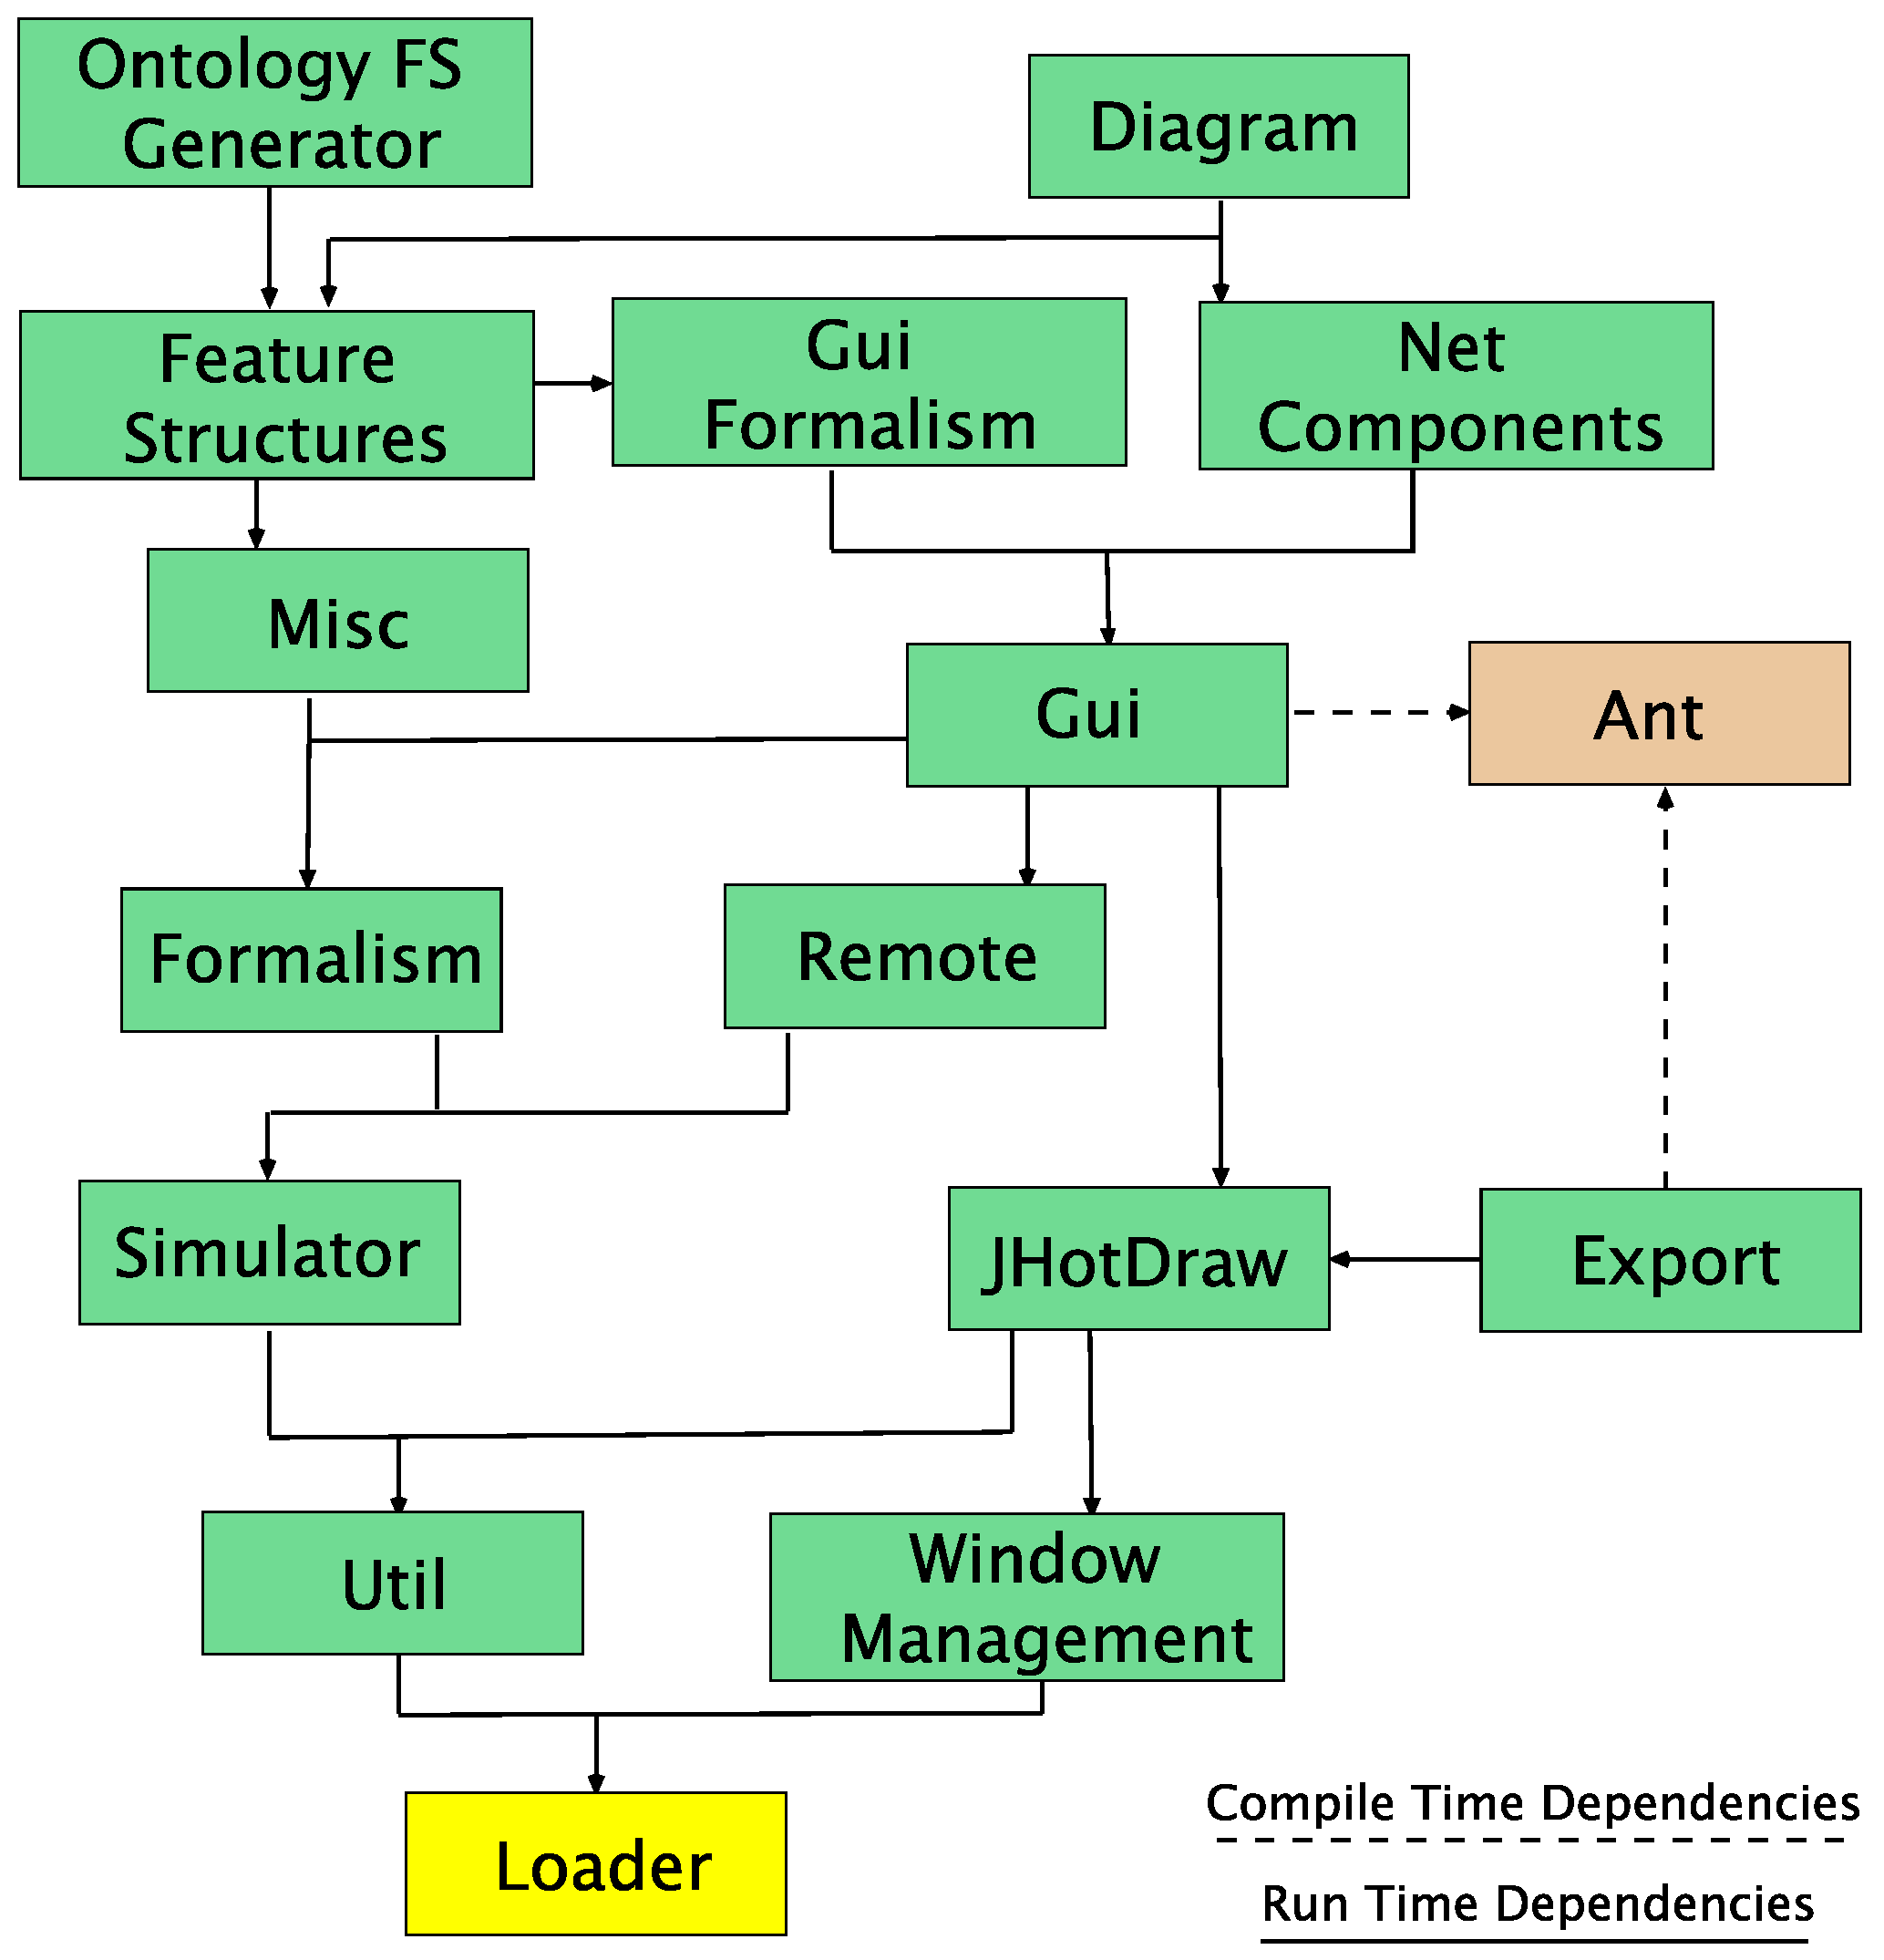
\includegraphics[width=0.6\textwidth]{material/images/settler-renew-tree-extend.pdf}
	  \caption{Minimale modulare Renew Version für Settler}
	  \label{fig:renew_mulan_plugins}
	\end{figure}	

	Im weiteren Fortgang müssen die Klassenpfade innerhalb der Mulan Plugins angepasst werden, denn diese verweisen auf Renew Plugins mit der alten Projektstruktur und werden daher nicht gefunden. Um diesen Zustand zu beheben, wird die Korrektur, mithilfe der regulären Ausdrücke, Mulan übergreifend nachgezogen und enthält zum Schluss keine Referenzen auf alte sowie nicht existierende Paketstrukturen von Renew. Die betroffenen Mulan Plugins sind: UseCaseComponents, YamlToFSConceptDiagram, KnowledgeRoundtrip, MulanDoc, FSOntologyGenerator, SLEditor, WF und das AgentRoleModeler Plugin. \newline
	Mit dem letzten Schritt wurden alle Mulan Java Klassen innerhalb der Renew Plugin Menge richtig verbunden, dennoch bestehen Probleme bei der Referenzierung der Aufrufmethoden. Wie in der Einleitung angedeutet, setzt das modulare Renew auf Renew mit erweiterten Benutzeroberfläche auf und wurde bislang nicht mit Mulan zusammengeführt. Aus diesem Grund kann die \textit{KnowledgeBaseGenerator} Klasse aus dem AgentRoleConverter Plugin nicht auf alle versprochenen Methoden von der erweiterten Benutzeroberfläche zugreifen, wie zum Beispiel das Ausführen eines Speicherdialogs. Dieses fehl Verhalten wird behoben indem Settler auf die angepasste Schnittstelle zugreift und das entsprechende Dialog koordiniert. \bigbreak

	\begin{figure}[h!]
	  \centering
	  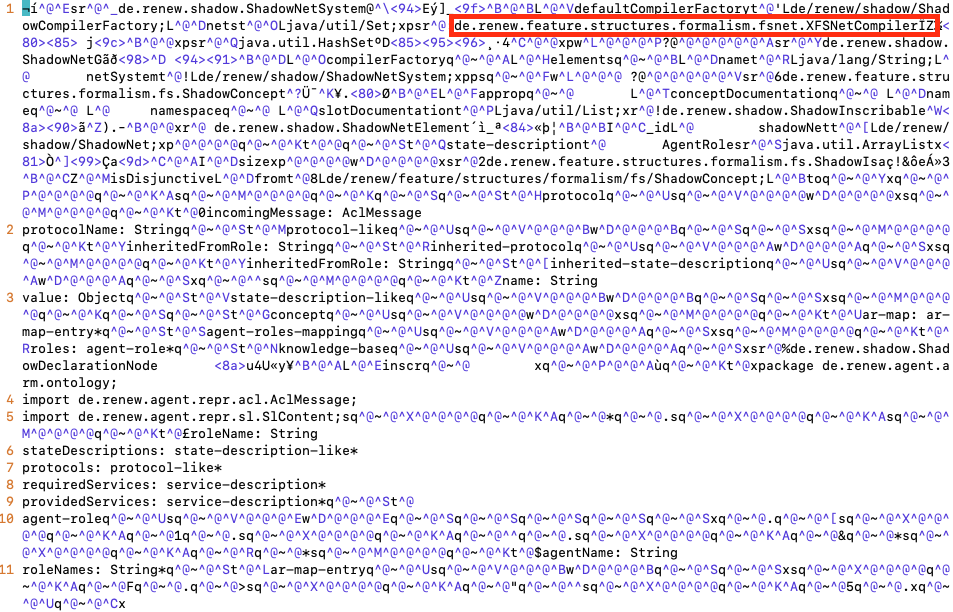
\includegraphics[width=0.8\textwidth]{material/images/shadownet.png}
	  \caption{SNS Netz}
	  \label{fig:sns_netz}
	\end{figure}

	Obwohl die Klassen sowie Methoden mit einander verzahnt wurden, müssen zusätzlich Ressourcen unter Verwendung des Ant Werkzeugs und speziell für Renew implementierte \textit{Ant Tasks} generiert werden. Diese nutzen Java Klassen, die in vielen Paketen der Renew Plugins direkt verankert sind. Somit müssen Ant Skripte für die entsprechenden \textit{Task's} adaptiert werden. Zum Beispiel in der \textit{commontasks.xml} für den \textit{CreateShadownetsTask}, der sich jetzt in einem anderen Paket befindet. Dieser ist zuständig für das Kompilieren der Renew Zeichnungen in ausführbare Shadow Netze. Auch wenn der \textit{CreateShadownetsTask} Shadow Netze aus den Renew Zeichnungen generieren kann, gibt es bereits kompilierte Netze die als einfache Ressourcen mit Mulan mitgeliefert werden. \newline
	Im Gegensatz zu den Renew Zeichnungen enthalten die Shadow Netze keine UI-Information, wie zum Beispiel Position oder Färbung der Netzelemente, jedoch enthalten diese Information über den genutzten Netz-Compiler, der für das Kompilieren der Datei zuständig war und für das Öffnen zuständig sein wird. Daher müssen bereits kompilierte Renew Zeichnungen für die modulare Renew Basis angepasst werde. Dafür wird mithilfe eines Text-Editors und einem regulären Ausdruck die entsprechenden Klassenverweise auf den \textit{XFSNetCompiler} aktualisiert, um den Ausführungskontext zu entsprechen. \newline
	Das Ergebnis sowie ein Beispiel für ein aktualisiertes Shadow Netz ist in der Abbildung \ref{fig:sns_netz} dargestellt. \bigbreak
	Zu diesem Zeitpunkt wurden alle Mängel und Uneindeutigkeiten zwischen Settler, Mulan und den modularen Renew beseitigt, dennoch fehlt für die Ausführung die Zeichnung \textit{settler.rnw}. Diese befindet sich im Settler Plugin Projekt und wird nicht in der Standardausführung mitgeliefert, sondern bei Bedarf mit einem \textit{sh} Skript während des Starts nachgeladen. \newline
	Da die Umsetzung auf Settler abzielt, wird dieses Skript im Ant \textit{build} Prozess verankert und in das Settler Plugin mit kompiliert und verpackt. \newline

	\begin{figure}[h!]
	  \centering
	  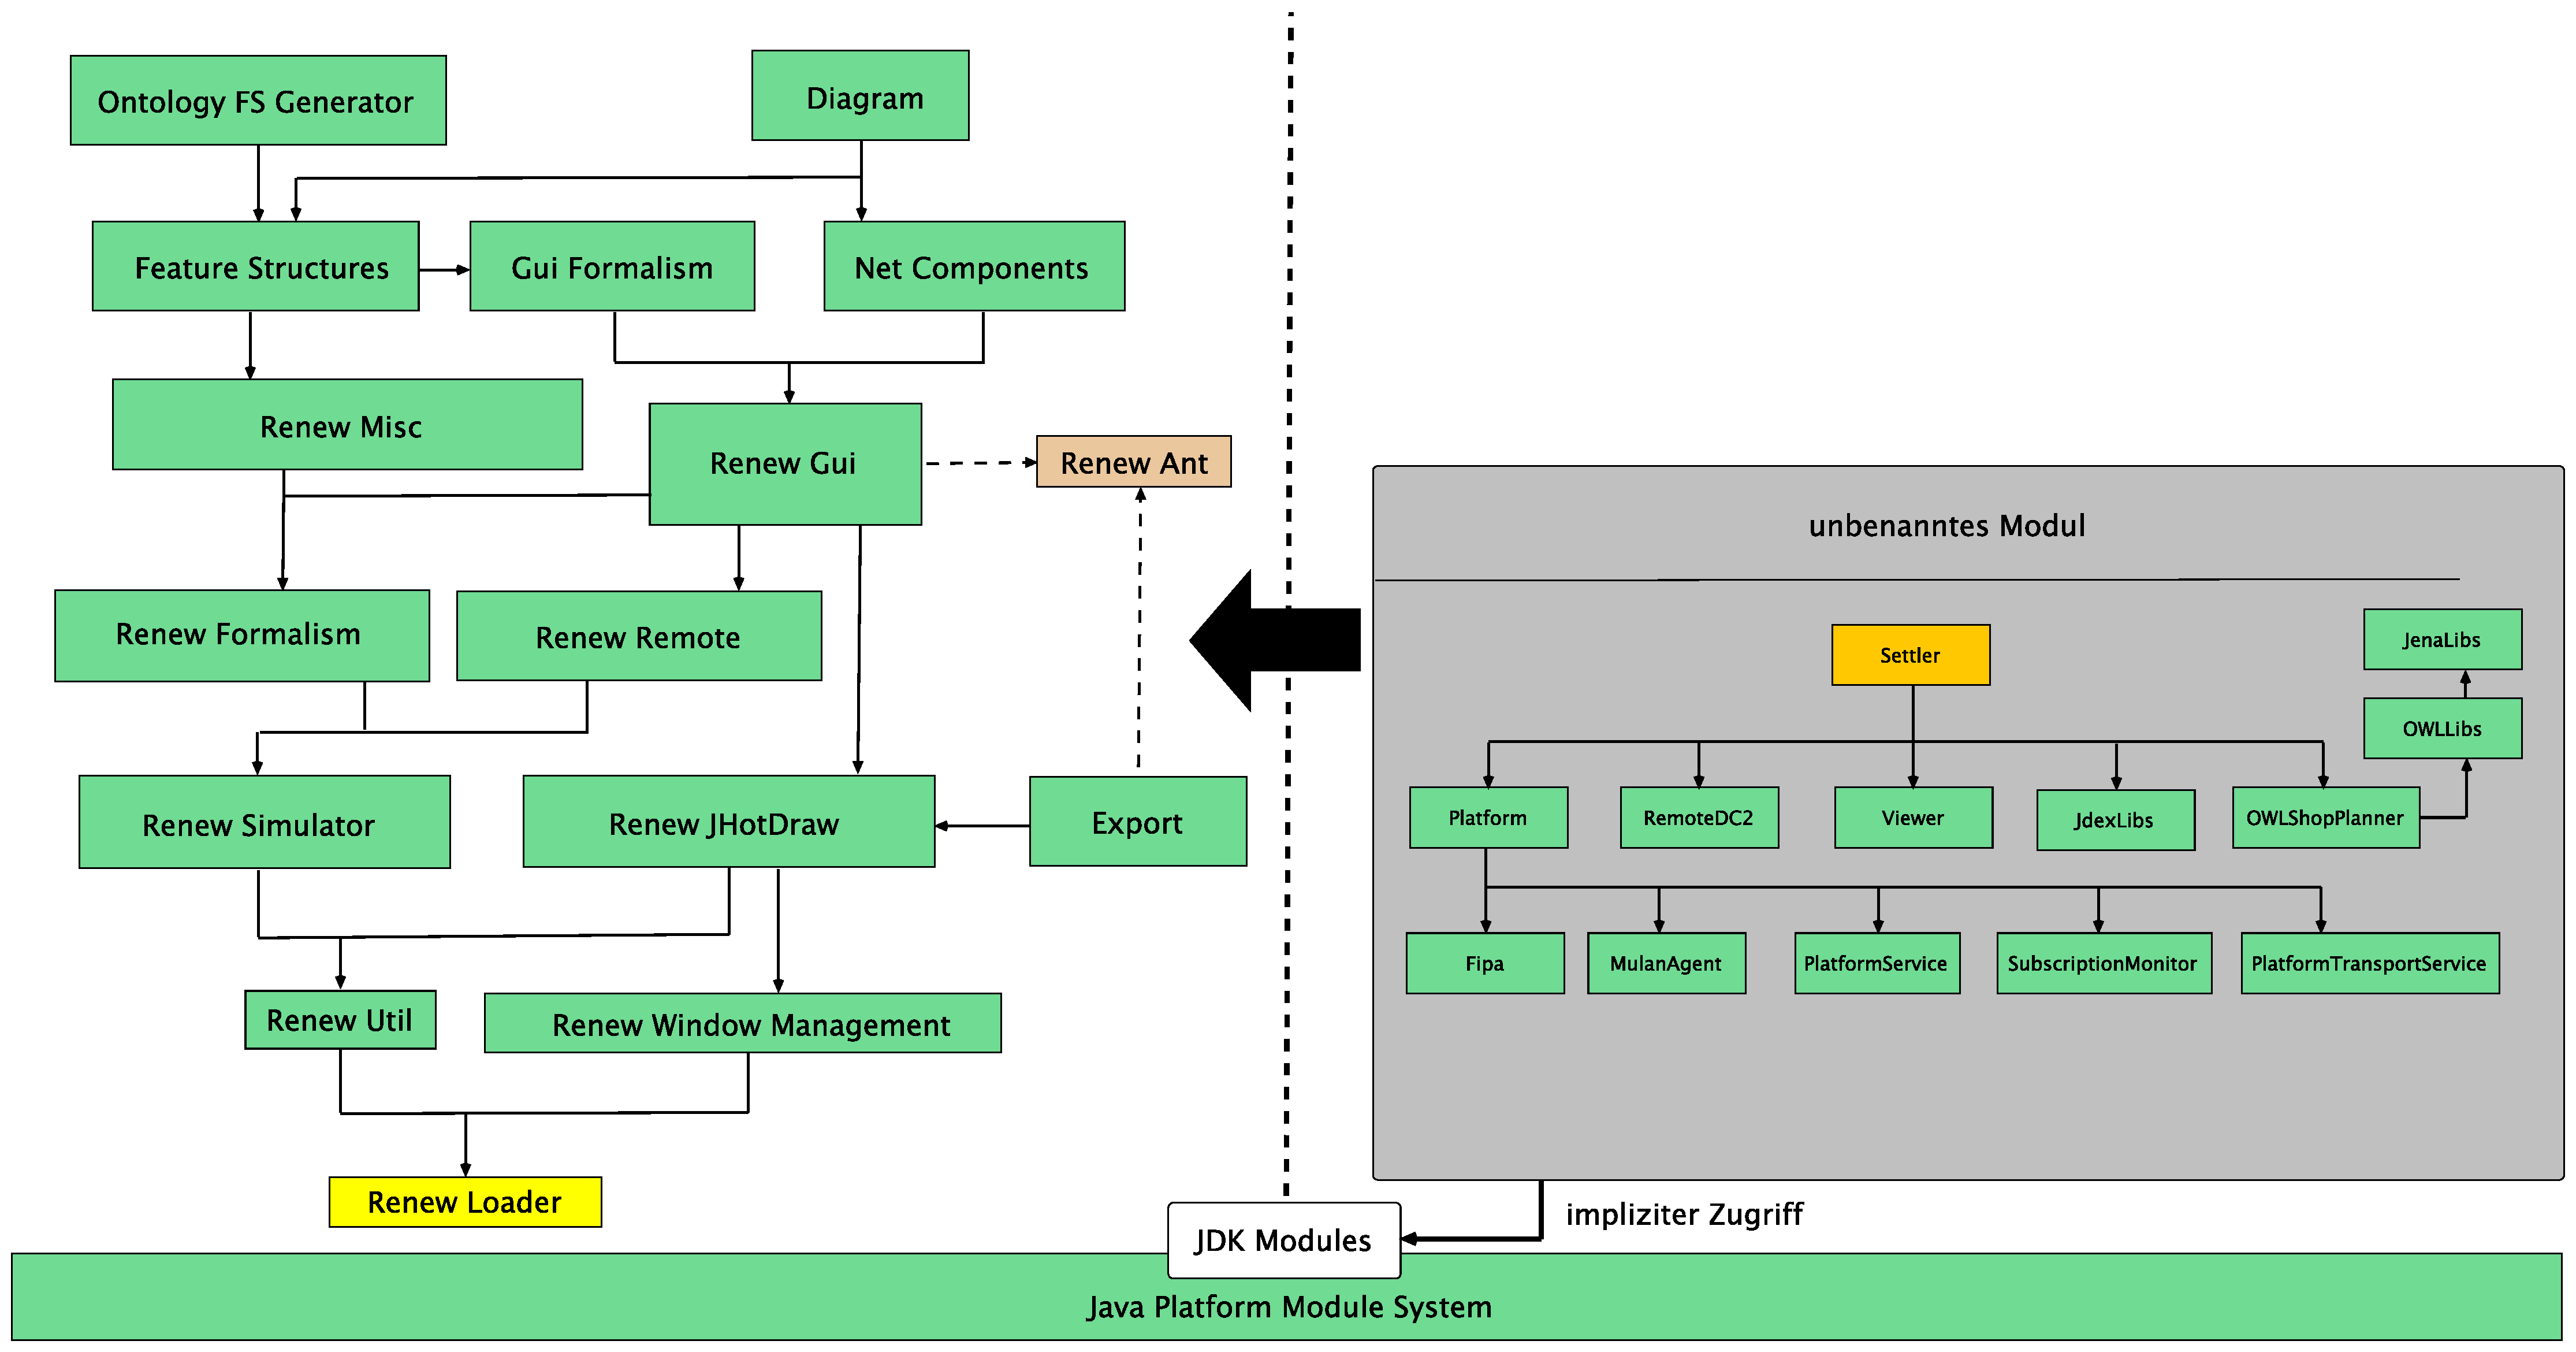
\includegraphics[width=0.84\textwidth]{material/images/settler-renew-mulan-vm.pdf}
	  \caption{Settler-Mulan Variation}
	  \label{fig:trans_config}
	\end{figure}

	Zusammengefasst ist das Settler Spiel bereit für die Ausführung und enthält alle nötigen Konfigurationen für das modulare Renew mit der erweiterten Oberfläche. Dafür wurden zahlreiche Anpassungen durchgeführt, die eine Brücke zwischen der Mulan-Settler Variation und dem modularen Renew bilden. Es wurden Plugins modularisiert, Ressourcen angepasst, Skripte umgeschrieben und kleine Mängel behoben. \newline
	In der Abbildung \ref{fig:trans_config} ist der fertige Prototyp abgebildet, der die Spezifikation erfüllt und als ein praktisches Beispiel für eine Migration einer existierender Software dient. 

\section{Evaluation}
	Der entstandenen Prototyp deckt ein Migrationsszenario ab, das innerhalb eines Projektes mit einer großen Codebasis entstehen könnte. Die Erwartung eines nahtlosen Austausch von Renew gegen das modulare Renew hat sich nicht ergeben. Alle Änderungen die im entstehenden Prototypen resultieren, deuten auf einen mittleren Arbeitsaufwand für das initiale Aufsetzen von existierendem Alt-Code auf modulare Grundlagen. Es müssen Pfade, Ressourcen und Prozesse angepasst werden, die voraussichtlich alle Bereiche eine Applikation betreffen werden.\newline
	Nichtsdestotrotz ergaben sich auch positive Resultate. Denn, das Erweitern der existierenden Modulmenge ergab ein einfaches, übersichtliches und nachhaltiges Verfahren, welches sich in der erweiterten Renew minimal Konfiguration erwiesen hat. Mit jedem weiteren modularisierten Plugin wurde das Hinzufügen von Plugins zu der Gesamtumsetzung immer simpler und verlangte keinen bis minimalen Aufwand für die benötigen Abhängigkeiten. Zusätzlich steigt ab einem gewissen Punkt die Unterstützung für das Koppeln der Module mit einer intelligenten IDE und bildet somit eine neues, willkommenes Hilfsmittel.
 
\chapter{Gesamt Evaluation}
Dieses Kapitel evaluiert die gesetzten Anforderungen aus der Anforderungsanalyse sowie der Anforderungsspezifikation und bewertet die Migration auf das Modulsystem von Java.\bigbreak	

% übergangn  


Für den Ersatz der veralteten Projektorganisation des Quellcodes wird die geforderte Projektstruktur in ein Maven Standard Layout überführt, welches den Java Code von den Java Compiler-Compiler Code trennt und die dazugehörigen Ressourcen separat verwaltet. Zusätzlich wurden die interne Struktur der Plugin Pakete, die sich mit anderen Plugins überschneiden aufgelöst und umbenannt, um den Java Anforderung des Modulpfades zu entsprechen. Darüber hinaus wurde ein Modulname eingeführt, der nach der Java Konvention mit den Organisations- oder Applikationsdomäne beginnt und mit den Feature Namen endet. Der neue Modulname fasst den Quellcode eines Moduls zusammen und ermöglicht das Erstellen zusätzlicher Module innerhalb eines Plugins, die ein gemeinsames Ziel verfolgen. Des Weiteren spiegelt der Modulname die interne Paketstruktur wieder und gestaltet die Codebasis Leserlich und Verständlich, da die Entwickler sofort ablesen können, aus welchen Modulen die Klassen stammen und für welchen Zweck diese entwickelt worden sind.\newline
Der Aufwand für die Umstrukturierung war wie erwartet groß, denn die Modernisierung der internen Struktur eines Elements aus einem gekoppelten Verband diverse Folgen für die Zugriffe auf dessen Ressourcen und Funktionalität mit sich bringt. Demnach müssen alle Zugriffe auf das Plugin angepasst, die \textit{import} Angaben Plugin-Weit überarbeitet und die existierende Meta-Information angeglichen werden. In Folge dessen wurden Änderungen nötig, die Plugin-Übergreifend aufgelöst werden müssen und über den Rahmen des Plugins hinausgehen. Dies führt zu Unsicherheit, da Änderungen in mehre als hundert Klassen entstehen und die Konsistenz der kompletten Applikation in Frage stellt. \newline
Im Endeffekt, ist die Umsetzung einer neuen Projektstruktur in einer ausgereiften Applikation eine wichtige und verantwortungsvolle Aufgabe, die  Nachhaltigkeit und Beständigkeit mit sich bringt.\bigbreak    

Während der Modularisierung des ersten Prototypen, der die kontinuierliche Migration abdeckt, wurde der gemischte Betrieb von modularisiertem \textsc{Renew} Code mit dem alt System betrachtet. Dementsprechend sollte die Migration nicht nur Module bilden und das Ergebnis begutachten, sondern auch die fortlaufende Integrität mit dem Altsystem inspizieren.\newline
Die Migration verfolgte den \textit{Chicken little} Ansatz und nutzte die von Java zur Verfügung gestellten Kommunikationsbrücke, die den Klassenpfad mit dem Modulpfad verbindet. Somit entstand kein zusätzlicher Aufwand für die manuelle Erstellung und die nachfolgende Qualitätskontrolle eines unentbehrlichen Elements. Da die Kommunikationsbrücke das Herzstück einer \textit{Chicken littel} Migration umsetzt, ist die benannte Kommunikationsbrücke ein begehrenswertes und willkommenes Ausstattungsmerkmal des Modulsystems von Java, die einen großen Teil des Migrationsszenarios übernimmt. Dementsprechend musste im Laufe der Migration nur auf die Adaption an die neue Umgebung geachtet werden, da die Kontext übergreifende Kommunikation sowie dessen Integrität bereits von Java zur Verfügung gestellt worden ist. \newline
Obwohl Java die Migration mit Migrationskonzepten unterstützt, entscheidet sie nicht in welchen Ablauf der Code Modularisiert werden soll. Daher wurden im Grundkapitel Konzepte vorgestellt, die nach der Größe einer Applikation Modularisierungsszenarien empfehlen. Für die \textsc{Renew} Modularisierung wurde das \textit{bottom up} Verfahren ausgewählt, da dieses als das präferierte Verfahren für gekoppelte Bibliotheksstrukturen gilt und sich gut auf das Plugin Konzept übertragen lässt. Das Verfahren modularisiert und integriert den Code, von den simplen bis zu den komplizierten Plugins, in das bestehende System und gliedert zusätzlich die Drittanbieter Bibliotheken als automatische Module ein.\newline 
Obwohl die bereits eingerichtete Projektstruktur und der Umsetzungsplan einen großen Teil der Modularisierung ausmachen, mussten die Plugins mit einer Schnittellenbeschreibung in Form einer \textit{module-info.java} ausgestattet werden, um als ein explizites Module gelten zu dürfen. Das Anreichern der ersten Plugins mit einer Modulbeschreibung geschieht mühelos, da die Konfigurationsdatei eine schlichte Schnittstellenbeschreibung besitzt, die nur das nötigste anfordert und nur wenig anbietet. Jedoch mussten diese während der gesamten Migration durchgehend nach gepflegt werden, da für jedes nachträglichen Plugin, Pakete in bereits modularisierten Plugin geöffnet werden mussten. Somit entstand ein fortlaufender Arbeitsaufwand beim Überarbeiten von bereits deklarierten Schnittstellen in den benötigten Plugins.\newline
Nichtsdestotrotz erwies sich die Durchführung als Vorbildhaft, denn die Abarbeitung der gesetzten Ziele und der entsprechenden Ausführungsschritte ergaben einen makellosen Weg vom bestehenden Altsystem auf das modernen Modulsystem von Java.\bigbreak

Als Konsequenz der Modularisierung von \textsc{Renew} samt der entsprechen Abhängigkeiten entsteht eine Applikation mit einem globalen übersichtlichen Abhängigkeitsgraphen, der die Evaluation der gesamten Konstruktion ermöglicht. Die Betrachtung ergab eine große Anzahl an transitiven Abhängigkeiten, die mithilfe des \textit{trantiv} Schlüssel auf eine reduziert Form des Abhängigkeitsgraphen runter gebrochen werden konnten und ergaben somit eine alternative Sicht auf die Plugin Konstellation. Der neue Abhängigkeitsgraph illustrierte eine natürliche Schichtenbildung von Plugins, die sich aus grundlegend bis zu erweiterten Fähigkeiten zusammensetzen. Des Weiteren impliziert die transitive Deklaration der Abhängigkeiten ihre Delegation an Module die dieses Nutzen möchten. In der Konsequenz kann der gesamte Kontext eines Plugins auf Plugins, die dieses erweitern, weitergereicht werden. \newline
Angelwand an die \textsc{Renew} Applikation, ist die transitive Deklaration der Modulabhängigkeiten eine großartige Erweiterung der Plugin Architektur, denn ab diesen Zeitpunkt wird der Kontext der zu erweiternden Plugins an den aufbauenden Plugin \textit{automatisch} weitergereicht, ohne dass die aufbauenden Plugins sich um die globale Struktur und Abhängigkeitsverwaltung kümmern müssen. Dazu gehören die Plugin Grundlagen, Drittanbieter Bibliotheken sowie die entsprechende Versionierung. \newline



\chapter{Schluss}


\section{Zusammenfassung}

Das Grundlagenkapitel behandelt das Arbeiten mit dem Klassenpfad auf der virtuellen Maschine von Java. Dazu gehören Konzepte wie der \textit{Classpath} und der \textit{Classloader} sowie \textit{Reflection} und die \textit{Interfaces}, die in der Umsetzung von \textsc{Renew} eine wichtige Rolle spielen. Dementsprechend werden Mechanismen vorgestellten, wie das Auffinden der Klassenaufenthaltsorte, das sichere Laden in die Virtuelle Maschine und das Arbeiten mit unbekannten Klassentypen.\bigbreak

In dem Kapitel der Modularisierung wurden wichtige Konzepte und Einschaften der Modularisierung erarbeitet, die in der Zukunft helfen sollen Module sauber zu entwerfen, zu erstellen oder zu bewerten. Dazu gehören kritische Modul Charakteristika, wie Modulkopplung, Modulbindung, Seiteneffektfreiheit, Modulgröße und Namensräume. \bigbreak

Mithilfe des Migrationskapitels werden zwei wesentliche Vorgehensweisen dargestellt, mit den eine Migration durchgeführt werden kann. Zusätzlich wird auf das Modulsystem von Java eingegangen, das eine bestimmte Vorstellung von einer Kontinuierliche Migration auf das Modulsystem besitzt. \newline
Die Migration des \textsc{Renew} Prototypen bediene sich dieser Idee und modularisiert die Plugins entsprechend dem \textit{bottom Up} Ansatzes. Darüber hinaus wurden wesentliche Modulsystem Migrationshürden benannt, welche die essenziellen Probleme zusammenfassen. \bigbreak

Das Kapitel der Analyse und Ausgangssituation vermittelt die Zielsetzung und den Umfang der Abschlussarbeit sowie die nachfolgende Durchführung. Es werden Gründe für eine Migration auf das Modulsystem von Java zusammengetragen, die daraus resultierenden Konsequenzen analysiert und anschließend die Anforderung an die bevorstehende Prototypen behandelt. Zum Schluss wird ein aktueller Zustand der \textsc{Renew} sowie \textsc{Mulan} Software konstruiert, die im Nachfolgenden mit einem Umsetzungsplan die gesetzte Spezifikation erreichen sollen.\bigbreak

In dem Kapitel des modularen \textsdc{Renew} Prototypen geht es um die Migration von \textsc{Renew} auf das Modulsystem von Java, die eine kontinuierliche und beispielhafte Migration demonstriert. Diese beinhaltet einen Umsetzungsplan, der die Projektstruktur reorganisiert, das Gradle Werkzeug für die Organisation des Projekts einführt und anschließend das Modulsystem von Java auf die vorbereitete Code-Basis aufsetzt. Zum Schluss folgt eine Evaluation, die den Prototypen auf das Modulsystem von Java optimal abstimmt und Parallelen mit dem Gradle Werkzeug zieht.\bigbreak
% proptotypen kapitel 

 Das Kapitel des \textsc{Mulan} Prototypen demonstriert mögliche Schwierigkeiten und den betreffenden Aufwand, der mit dem Austausch einer grundlegend Basis-Software in einem größeren System auftreten können. Da das Rahmenwerk \textsc{Mulan} auf dem \textsc{Renew} Simulator aufsetzt und ohne diesen nicht betriebsfähig ist, ist \textisc{Mulan} komplett an \textsc{Renew} während der Kompilation sowie der Laufzeit angewiesen. Daraus folgen Referenz- und Zugriffsschwierigkeiten, die Global behoben werden müssen. Zusätzlich wird mit diesem Prototypen eine Übergangsszenario Simuliert, das \textsc{Renew} mit dem Gradle Werkzeug und \textsc{Mulan} mit dem Ant Werkzeug zugleich eine funktionierendes Ergebnis liefern. \bigbreak

 Zum Schluss wird das Ergebnis der Abschlussarbeit evaluiert, zusammengefasst und der Ausblick für die mögliche Forschung und Ausbau der Prototypen gegeben. 


\section{Ausblick} 



\newpage

- Migtation Einleitungssatz 
- Evaluation des Migrationsablaufes
	- was wurde dafür getan (modul info)
	-  nicht alle charactersitica von den good practice müssen umgesetzt werden
	- wie wurde es getan (automatische expletize unbenannte module ( verweise auf Grundlagen Kapitel))
	- was für folgen hatte sie (Konfiguration, Transitivität,Kontext, Schichten(Nattürliches ereigniss(hat sich selbst entwicklet)))
	- Mehrwert  sichtbar ?



% PROJEKTSTRUKTUR 
	% ^-> Anforderungen aus der Modularisierung 
	% -> Probleme die aufgetaucht sind. erwartet, unerwartet, kritik an das Projekt, lob an das Projekt  (pafad umbau lässt)
	% -> Was bringt es auf lange Sicht -> erweiterbarkeit war die anforderung (Mehr module im Plugin) 
	% ^-> Unerwartete mängel wurden behoben ->  stark veraltete und auf zeit unsauberer Projekt aufbau (bilder, resourcen, unterschieldiche Klassen typen und für verschiedenen zweck  im sleben Packet) 
	% ^-> Konvention der modulanamengenbunf, das auf den source aufbau hinweist 
	% -> es Felen konventionen die in der AUssicht näher beschprochen werden 
	% ^-> Konsistenz gegeben, sind die verädnerungen kritisch (Ohne kla defenierte schnissteleln ja (keine schnittstellen verwaltung also ja))?
	% AUFWAND FÜR DIE UMSTRUKTURIERUNG

% MODULARISIERUNG
% -> Modularisierung von  passenden Strukturen sehr einfach aber auch sehr schwer.  Auslesen der zugriffe auf das Modul kahn sehr Müsehlig sein und muss plugin weit getestet und angepasst werden
% -> Die Migration von Modulaen gelingt ohne probleme, jedes MIgrationsszenario kann mit Hilfe der Expliziten automatischen unbenannten und offenen Module abgedeckt werden. Besonders positiv fiel das automaotsiche modul auf, dass  für den Klassenpfad und für den Modulpfad zugägnlich ist und Bausteine einer Bibliothke, schritt für schritt modularisieren lässt.  Modularisierung nicht nur der Code Base sondern der Arbhängigkeiten in kleien Schritten möglich. 
% -> Die Transitive Konfiguration in einem Modulsystem hat einen erheblichen Postivien einfluss auf die Pluginkopplung( Plugin Schichten (Kontexte/ Abhängigkeiten) werden transitiv wietergereicht ohne Komplikation oder verstündniss oder aurbeitsaufwand für aufgliegende module )
% -> Was kan der Prototyp leisten ? wie weit geht die Unterstützung lan  man ihn an weitere Studenten delegieren. tut es was ich versprochen habe 
% -> Konsequenzen für \textsc{Renew} und allgemein für appliaktionen ( was hat \textsc{Renew} erlebt was wird allen zustoßen)
% -> Mehrwert ist da oder nicht ? was kann man mit dem modulsystem von java erreichen
% MODULARISIERUNG \textsc{Mulan} 
% Wleche seite der Modualriseirung hat \textsc{Mulan} gezeigt 
% -> AUFWAND FÜR DSIE MODULARISIERUNG



% GRADLE
% Hat sich das Gradle wärkzueg behauptet ? 
% verstädnlichkeit, 
% code menge, 
% erweiterbarkeit, 
% konfiguration , 
% mehrwert in der nutzung 




% Anforderungsanalyse/Spezifikation
%- Anforderung an Modulariserte Systeme 
%- Charakterisierung (Aufbau Schnittstellen Umfang)
%- Aufwand für Modularisierung
%- Konsequenzen (Zyklen , Splitt Packages ,Alte APIEs)
%- Konsistenz 
%- Mehrwert
%
%- Übergangsphase Aufwand 
%
%- Gradle -> Projektstruktur 
%- Zusätzliche Module Unterstützen 
%- gelöst von der Entwiklungsumgebung 
%- kohärente Arbeitsweise
%- ältere Verfahren 




% Evaluaiere die Anfprderungsanalyse Übergeordnete Kritik 
% Hat sich das Gradle wärkzueg behauptet ? verstädnlichkeit, code menge, erweiterbarkeit, konfiguration , mehrwert in der nutzung 
% Modularisierung konsequenzen für Systeme 
% 

% Was wollte ich erreichen 
% Unterziele 
% Bewertung der Unterziehle 




% Was habe ich erreicht 



\blankpage
      
\begin{appendices}
	%\chapter{Glossary}
\label{appendixA}
Just comment \verb|\chapter{Glossary}
\label{appendixA}
Just comment \verb|\chapter{Glossary}
\label{appendixA}
Just comment \verb|\input{AppendixA-Glossary.tex}| in Masterthesis.tex if you don't need it!

\begin{longtable}{p{2.5cm}p{9.5cm}}

\huge{\textbf{Symbols}}& \\
\hline
\\
\$ & US. dollars. \\
\\
\\
\huge{\textbf{A}}& \\
\hline
\\
A& Meaning of A.\\
\\
\\
\huge{\textbf{B}}& \\
\hline
\\

\\
\\
\huge{\textbf{C}}& \\
\hline
\\

\\
\\
\huge{\textbf{D}}& \\
\hline
\\

\\
\\
\huge{\textbf{E}}& \\
\hline
\\

\\
\\
\huge{\textbf{F}}& \\
\hline
\\

\\
\\
\huge{\textbf{G}}& \\
\hline
\\
\\
\\
\huge{\textbf{H}}& \\
\hline
\\

\\
\\
\huge{\textbf{I}}& \\
\hline
\\

\\
\\
\huge{\textbf{J}}& \\
\hline
\\

\\
\\
%\huge{\textbf{K}}& \\
%\hline
%\\
%\\
%\\
%\huge{\textbf{L}}& \\
%\hline
%\\
%\\
%\\
\huge{\textbf{M}}& \\
\hline
\\

\\
\\
\huge{\textbf{N}}& \\
\hline
\\

\\
\\
%\huge{\textbf{O}}& \\
%\hline
%\\
%\\
%\\
\huge{\textbf{P}}& \\
\hline
\\

\\
\\
\huge{\textbf{Q}}& \\
\hline
\\

\\
\\
\huge{\textbf{R}}& \\
\hline
\\

\\
\\
\huge{\textbf{S}}& \\
\hline
\\

\\
\\
\huge{\textbf{T}}& \\
\hline
\\

\\
\\
\huge{\textbf{U}}& \\
\hline
\\

\\
\\
\huge{\textbf{V}}& \\
\hline
\\

\\
\\
\huge{\textbf{W}}& \\
\hline
\\

\\
\\
\huge{\textbf{X}}& \\
\hline
\\

\\
\\
%\huge{\textbf{Y}}& \\
%\hline
%\\
%\\
%\\
%\huge{\textbf{Z}}& \\
%\hline
%\\
%\\
%\\
\end{longtable}



| in Masterthesis.tex if you don't need it!

\begin{longtable}{p{2.5cm}p{9.5cm}}

\huge{\textbf{Symbols}}& \\
\hline
\\
\$ & US. dollars. \\
\\
\\
\huge{\textbf{A}}& \\
\hline
\\
A& Meaning of A.\\
\\
\\
\huge{\textbf{B}}& \\
\hline
\\

\\
\\
\huge{\textbf{C}}& \\
\hline
\\

\\
\\
\huge{\textbf{D}}& \\
\hline
\\

\\
\\
\huge{\textbf{E}}& \\
\hline
\\

\\
\\
\huge{\textbf{F}}& \\
\hline
\\

\\
\\
\huge{\textbf{G}}& \\
\hline
\\
\\
\\
\huge{\textbf{H}}& \\
\hline
\\

\\
\\
\huge{\textbf{I}}& \\
\hline
\\

\\
\\
\huge{\textbf{J}}& \\
\hline
\\

\\
\\
%\huge{\textbf{K}}& \\
%\hline
%\\
%\\
%\\
%\huge{\textbf{L}}& \\
%\hline
%\\
%\\
%\\
\huge{\textbf{M}}& \\
\hline
\\

\\
\\
\huge{\textbf{N}}& \\
\hline
\\

\\
\\
%\huge{\textbf{O}}& \\
%\hline
%\\
%\\
%\\
\huge{\textbf{P}}& \\
\hline
\\

\\
\\
\huge{\textbf{Q}}& \\
\hline
\\

\\
\\
\huge{\textbf{R}}& \\
\hline
\\

\\
\\
\huge{\textbf{S}}& \\
\hline
\\

\\
\\
\huge{\textbf{T}}& \\
\hline
\\

\\
\\
\huge{\textbf{U}}& \\
\hline
\\

\\
\\
\huge{\textbf{V}}& \\
\hline
\\

\\
\\
\huge{\textbf{W}}& \\
\hline
\\

\\
\\
\huge{\textbf{X}}& \\
\hline
\\

\\
\\
%\huge{\textbf{Y}}& \\
%\hline
%\\
%\\
%\\
%\huge{\textbf{Z}}& \\
%\hline
%\\
%\\
%\\
\end{longtable}



| in Masterthesis.tex if you don't need it!

\begin{longtable}{p{2.5cm}p{9.5cm}}

\huge{\textbf{Symbols}}& \\
\hline
\\
\$ & US. dollars. \\
\\
\\
\huge{\textbf{A}}& \\
\hline
\\
A& Meaning of A.\\
\\
\\
\huge{\textbf{B}}& \\
\hline
\\

\\
\\
\huge{\textbf{C}}& \\
\hline
\\

\\
\\
\huge{\textbf{D}}& \\
\hline
\\

\\
\\
\huge{\textbf{E}}& \\
\hline
\\

\\
\\
\huge{\textbf{F}}& \\
\hline
\\

\\
\\
\huge{\textbf{G}}& \\
\hline
\\
\\
\\
\huge{\textbf{H}}& \\
\hline
\\

\\
\\
\huge{\textbf{I}}& \\
\hline
\\

\\
\\
\huge{\textbf{J}}& \\
\hline
\\

\\
\\
%\huge{\textbf{K}}& \\
%\hline
%\\
%\\
%\\
%\huge{\textbf{L}}& \\
%\hline
%\\
%\\
%\\
\huge{\textbf{M}}& \\
\hline
\\

\\
\\
\huge{\textbf{N}}& \\
\hline
\\

\\
\\
%\huge{\textbf{O}}& \\
%\hline
%\\
%\\
%\\
\huge{\textbf{P}}& \\
\hline
\\

\\
\\
\huge{\textbf{Q}}& \\
\hline
\\

\\
\\
\huge{\textbf{R}}& \\
\hline
\\

\\
\\
\huge{\textbf{S}}& \\
\hline
\\

\\
\\
\huge{\textbf{T}}& \\
\hline
\\

\\
\\
\huge{\textbf{U}}& \\
\hline
\\

\\
\\
\huge{\textbf{V}}& \\
\hline
\\

\\
\\
\huge{\textbf{W}}& \\
\hline
\\

\\
\\
\huge{\textbf{X}}& \\
\hline
\\

\\
\\
%\huge{\textbf{Y}}& \\
%\hline
%\\
%\\
%\\
%\huge{\textbf{Z}}& \\
%\hline
%\\
%\\
%\\
\end{longtable}



\blankpage
	% \chapter{Cassandra}
\label{appendix:Cassandra}
Cassandra ist eine NoSql Datenbank, die nach dem Wide-Column Model konzipiert ist. Cassandra vereint verschieden Eigenschaften von Googles BigTable \cite{bigtable} und Amazons Dynamo \cite{dynamo}. Sie wurde 2010 von Facebook entwickelt, um das Inbox Search Problem zu lösen \cite{cassandra}. Es ist eine verteilte Datenbank, die sich unter dem CAP-Theorem als AP charakterisieren lässt, wobei man das Level an Konsistenz manuell einstellen kann.

\section{Daten Model}
\label{sec:DM}
Das Daten Modell von Cassandra entspricht dem von BigTable, also dem Wide-Column Modell. Dies beruht im Wesentlichen, wie alle Arten an NoSql Datenbank Modellen auf Key-Value-Stores. Dabei wird für einen Primary Key jeweils eine Reihe mit Column-Families definiert. Die Column-Families bestehen wiederum aus einem Key, der sie beschreibt, und einem Value der dann den Wert angibt. Der Wert kann allerdings wieder eine Menge an Column-Families sein, wodurch es möglich ist Column-Families beliebig zu verschachteln. Es wird bei der Initialisierung angegeben welchen Typ der Wert hat, Verschachtlung wird über benutzerdefinierte Typen erzeugt.
\begin{figure}[htbp!]
	\centering
	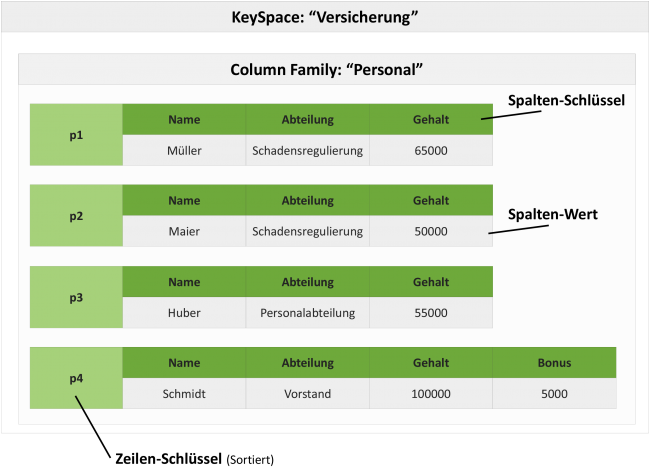
\includegraphics[scale=0.45]{pics/colfam.png}
	\figuresource{\url{http://wi-wiki.de/doku.php?id=bigdata:spaltendb}}
	\caption{Beispiel Daten Modell}
	\label{fig:bspDM}

\end{figure} Column-Families, die wiederum Column-Families beinhalten, bezeichnet man als Super-Column-Families. Bei Cassandra werden bei der Initialisierung einer Tabelle, die auch nichts anderes ist als eine Super-Column-Family, alle möglichen Column-Families angegeben. Sie definiert darüber hinaus den Primary Key über den auf die Werte der Column-Families zugegriffen werden können. Im Unterschied zu herkömmlichen SQL Tabellen ist es aber möglich Werte für diese zu unterschlagen, wie in Abbildung \ref{fig:bspDM} für p1 - p3 dargestellt.\\ 
Ein KeySpace stellt die oberste Schicht des Datenmodells dar. Für den KeySpace werden bei der Initialisierung eine Replikationsstrategie und eine Anzahl Replikas angegeben, die zu erstellen sind. Diese gelten dann für alle Tabellen, die unter dem KeySpace erstellt werden.

\section{System}
Implementiert ist Cassandra in Java. Darauf aufbauend sind auch die Basis Java Typen verfügbar. Die Daten werden von Cassandra redundant auf verschiedene Instanzen verteilt. Systemnachrichten werden dabei über UDP verschickt, Anwendungsnachrichten, also Nachrichten, die mit den Daten zu tun haben, per TCP um den Verlust von Nachrichten zu vermeiden. Bei den Systemnachrichten ist dies zu verkraften.

\subsection{Partitionierung}
Die Partitionierung orientiert sich an der von Dynamo \cite{dynamo}. Cassandra benutzt genauso wie Dynamo Consistent-Hashing, um Daten auf die verschiedenen Instanzen zu verteilen. Dabei erhalten die verschiedenen Instanzen einen Wert, der sie uniform über einen vordefinierten Wertebereich verteilt, wie in Abbildung \ref{fig:uniformHashing} abgebildet. Consistent-Hashing macht aus dem Wertebereich einen Ring, über den dann die Daten auf die Instanzen wie folgt verteilt werden. Aus einem Datum wird über die Hashfunktion ein Hash-wert berechnet. Das Datum wird dann auf der Instanz abgespeichert, deren Wert auf dem Ring aufsteigend als nächstes kommt. Dieses Verfahren kann zu einer ungleichen Verteilung der Daten auf die Instanzen führen, sodass dadurch die Performance des Systems ineffizient wird. Cassandra löst diese Problem anders als Dynamo dadurch, dass die Werte der Instanzen an die Verteilung der Daten angepasst werden, wie in Abbildung \ref{fig:adaptedHashing} dargestellt. So sind zwar einige Instanzen für einen größeren Wertebereich zuständig, andererseits kommen in diesem größeren Wertebereich weniger Daten vor, sodass die Daten uniform auf die Instanzen verteilt werden. Wird der Datensatz zu groß, skaliert Cassandra, indem eine Instanz im Consistent-Hashing Ring zwischen den Knoten mit den meisten Daten eingefügt wird. Danach werden die Bereiche wieder so angepasst, dass alle Instanzen ungefähr gleich belastet sind.
\begin{figure}[htbp!]
	\centering
	\begin{subfigure}[c]{0.49\textwidth}
		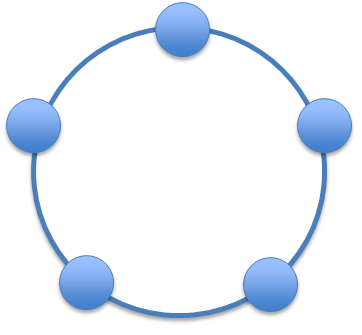
\includegraphics[scale=0.5]{pics/uniformHashing.png}
		\subcaption{Consistent-Hashing uniform distributed instances}
		\label{fig:uniformHashing}
	\end{subfigure}
	\begin{subfigure}[c]{0.49\textwidth}
		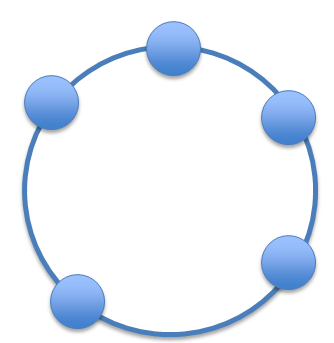
\includegraphics[scale=0.5]{pics/adaptedHashing.png}
		\subcaption{Consistent-Hashing adapted distribution of instances}
		\label{fig:adaptedHashing}
	\end{subfigure}
	\caption{Consistent-Hashing Ring}
\end{figure}

\subsection{Replikation}
Die Art der Replikation in Cassandra ist vom Benutzer konfigurierbar. Die Anzahl der Replikas und die Replikationsstrategie wird durch den KeySpace festgelegt. Dabei kann man zwischen SimpleStrategy und NetworkTopologyStrategy auswählen. Die SimpleStrategy repliziert ohne auf die Netzwerkstruktur einzugehen. Somit beugt sie weniger stark potentiellem Datenverlust vor und sollte daher nur für Test-Zwecke benutzt werden. Sei N die Anzahl Replikas, werden die Daten immer auf die N-1 Nachfolgeknoten repliziert. Bei der NetworkTopologyStrategy wird die Hierarchie von Datacentern und drin enthalten Racks bei der Verteilung betrachtet wird. Somit wird diese Strategie auch für das Deployment empfohlen. Innerhalb dieser Strategie kann man sich wiederum zwischen Rack Aware und Datacenter Aware entscheiden. Dabei werden die Replikas entweder auf verschiedene Racks oder Datacenter verteilt, um die höchst mögliche Datensicherheit zu gewährleisten. Diese Strategien beziehen sich auf den Koordinator, also die Hauptinstanz einer Partition von Daten, da dieser für die Replikation zuständig ist.
Bei der Bestimmung eines Koordinators wird Zookeeper verwendet. Dadurch sind alle Netzwerkänderungen und -konfigurationen persistent gespeichert, da Zookeeper die Konfigurationen jedes Knotens automatisch persistent speichert. Zur Kommunikation werden bei Zookeeper Gossip Algorithmen verwendet.

\subsection{Persistenz}
Persistenz erreicht Cassandra über ein ähnliches System wie BigTable \cite{bigtable}. Zunächst gibt es die MemTable, die im Hauptspeicher gehalten wird und als Cache fungiert. Sie besitzt eine Konfiguration einer Schranke, ab der die MemTable auf die Platte persistiert wird. Auf der Platte gibt es die SSTable, Bloom Filter, index file, compression file und statistics file. Die Daten werden in eine SSTable geschrieben, also eine eigene Datei geschrieben, wenn sie noch nicht vorhanden sind. Wenn dies nicht der Fall ist, wird der betreffende Teil einer SSTable in die MemTable geladen, alle Operationen ausgeführt und die Daten wieder zurück auf die Platte geschrieben. Der Bloom Filter verhindert unnötige Lookups in nicht relevante SSTables. Der Index beschleunigt den Lookup innerhalb einer SSTable. Damit man nicht viele kleine SSTable-Dateien hat werden zwei SSTable, durch einen merge-Prozess immer dann zusammengefasst, wenn eine mindestens halb so groß ist wie die andere. Vorhandene SSTable Files können zusätzlich noch komprimiert werden.

\section{CQL}
Mit CQL (Cassandra Query Language) gibt es eine auf Cassandra zugeschnittene SQL-ähnliche Abfragesprache, die es den Anwendern konventioneller Datenbanken deutlich leichter macht mit Cassandra zu arbeiten. Dabei ist es wichtig zu wissen, dass CQL bei weitem nicht so ausdrucksstark ist wie SQL. Das liegt daran, dass CQL im wesentlich eine abstrakte API für das Cassandra Datenmodell darstellt. In CQL sind normale Datenbank Typen wie int, text, etc. möglich, allerdings kann man auch von Collections wie List, Set und Map Gebrauch machen, da es dafür direkte Java Typen gibt. Des Weiteren ist es möglich eigene Typen zu definieren, wie schon in Abschnitt \ref{sec:DM} beschrieben.\\
\begin{figure}[htbp!]
	\centering
	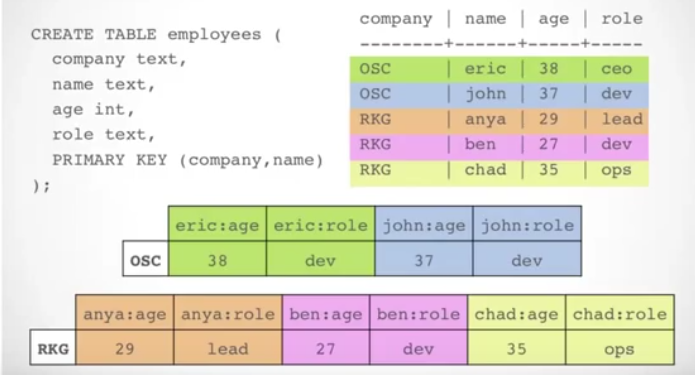
\includegraphics[scale=0.7]{pics/cql_mapping.png}
	\figuresource{\url{https://www.youtube.com/watch?v=UP74jC1kM3w}}
	\caption{CQL Mapping}
	\label{fig:mapping}
\end{figure}
Tabellen und Spalten werden wie ebenso in Abschnitt \ref{sec:DM} beschrieben durch Column-Families dargestellt. und wie in SQL erzeugt. Dabei wird ein Primary Key benötigt, der dann als Row Key fungiert. Es kann nur über diesen Row Key auf die Zeilen zugegriffen werden. Deshalb kann man in der WHERE-Klausel in CQL auch nur Elemente des Primary Key angeben. Auf diesen Elementen wird durch die Indizierung schon beim Speichern in Cassandra eine Sortierung berechnet was die Anfragen deutlich perfomanter macht. Für alle anderen Spalten der Zeile wäre dies also nicht performant und wird von CQL nicht gestattet. Die Spalten und Zeilen werden wie folgt auf das Cassandra Datenmodell abgebildet.\\
Der erste Teil des Primary Keys bildet, wie man sehen kann, den Row Key, die restlichen Teile werden mit ihren Werten in die Beschreibung der Column-Families integriert, so wie im unteren Teil in Abbildung \ref{fig:mapping} beschrieben. Somit werden alle Zeilen mit dem gleichen ersten Teil des Primary Keys in der gleichen Zeile abgespeichert. Über dieses Mapping ist es möglich eine tabellenartige Abstraktion zu erzeugen, die sich durch CQL ausdrückt und Anwendern ein aus SQL bekanntes Interface bietet.

	% \chapter{Big Table}
\label{bigTable}
Some text.

\section{Einführung}
Täglich kommen mehrere Petabytes an Daten von über 60 Google Anwendungen zusammen. Dafür verantwortlich sind mehr als 1000 Computer die untereinander vernetzt sind. Um diese Daten verwalten zu können wurde Bigtable ins Leben gerufen. Das Ziel der Datenbank war es in vielen Bereichen anwenden zu können. Dazu sollte es Skalierbar sein sowie eine hohe Performance und Verfügbarkeit besitzen.


\section{Datenmodell}
Bigtable ist eine verteiltes, persistentes multidimensionale sortierte Map. Diese Map ist indexiert über eine row key, columen key und einem timestamp. Jeder Wert in dieser Map ist ein Array mit Bytes. Das folgende Datenmodell soll eine Speicherung von Webseiten veranschaulichen.

\begin{figure}[!htpb]
	\centering
	\includegraphics[]{pics/bigtable_schema.png}
	\caption {Tabellen Beispiel}	
\end{figure}

Das Datenmodell besteht aus zwei Familien dem Inhalt und den Ankerpunkten. Die erste Familie beinhaltet den Inhalt der Webseite, mit drei unterschiedlichen Zeitstempeln (t3,t5,t6). Drei unterschiedliche Zeitstempeln bedeutet, dass die Website www.cnn.com in drei unterschiedlichen Versionen abgespeichert wurde. Die Anker Familie beinhaltet jeweils nur eine Version. Den Anker mit „CNN.com“ mit dem Zeitstempel t8 und dem Anker „CNN“ mit dem Zeitstempel t9. 
 
\paragraph{Rows}
Bigtable speichert Daten in lexikopgrahischer reihenfolge und sortiert diese nach Zeilen. Eine row range beinhaltet alle gleichnamigen URL’s, so dass alle mit der gleichen Domain zusammen abgespeichert werden. Das vereinfacht die Analyse und das Hosting der gleichnamigen Domains und macht dies zudem effizienter.

\paragraph{Column families}
Verschieden column keys werden in eine gemeinsame Gruppe gespeichert. Das nennt man column families. Alle Daten, welche in der gleichen Gruppe gespeichert werden sind vom gleichen typ. Bevor Daten in einer Gruppe gespeichert werden können, muss diese column family als erstes erstellt werden.

\paragraph{Timestamp}
Jede Zelle in Bigtable kann mehrere Versionen der gleichen Daten beinhalten. Dieser Versionen werden indexiert durch den Zeitstempel (timestamp). Der Zeitstempel ist bis auf die Micro Sekunde genau. Durch die „two per-column-family“ kann der Benutzer festlegen, wie viele Versionen der gleichen Daten gespeichert werden sollen. Alle weiteren Versionen werden automatisch gelöscht.

\paragraph{API}
Die API von Bigtable ermöglicht das erstellen und löschen von Tabellen und Spaltennamen, sowie das ändern von Tabellen, Cluster und Metadaten einer Spaltenfamilien. Das folgende Codebeispiel wurde in C++ geschrieben und Verändert den Inhalt der Tabelle Webtable. 

\begin{figure}[!htpb]
	\centering
	\includegraphics[]{pics/bigtable_api.png}
	\caption {Zugriffs Beispiel mit der BigTable API}	
\end{figure}

Der Code verändert die Spalte „com.cnn.www“ und fügt einen neuen Anker hinzu. Im nächsten Schritt wird ein vorhandener Anker „anchor:www.abc.com“ gelöscht und festgeschrieben.


\paragraph{Building Blocks}
Bigtable ist auf mehreren anderen Teilen der Google-Infrastruktur aufgebaut. Zum Beispiel benutzt Bigtable das verteilte Google File System (GFS). Welches für die Speicherung von Logs und Daten verantwortlich ist. Ein Bigtable Cluster operiert typischerweise auf einem verteilten Pool von Computern. Auf diesem Pool laufen eine breite sparte von verschiedenen Anwendungen. Bigtable basiert auf einem Cluster Management System für Zeit-Planung-Jobs, Ressourcenmanagements auf geteilten Computer, agieren mit Computerfehlern und dem Anzeigen des Computer Status. Das SSTable Format stellt eine persistente, geordnete unveränderliche Abbildung von Schlüsseln zu Werten zur Verfügung, wobei sowohl Schlüssel als auch Werte willkürliche Bytefolgen sind. Operationen werden bereitgestellt, um den Wert zu suchen, der einem bestimmten Schlüssel zugeordnet ist.

\paragraph{Implementation}
Bigtable besteht aus drei Haupt Komponenten, einer Bibliothek, einem Master Server und vielen weiteren tablet servern. Die Bibliothek ist in jeden Client verlinkt, somit kann der Client auf alle Funktionen zugreifen. Der Master Server wird zufällig ausgewählt. Dieser teilt den tablet servern die tablets zu. Außerdem ist für die Verteilung der Lasten zuständig und ist für die garbage collection. Sobald eine Tabelle zu groß wird, wird diese von einem tablet server gesplittet. So wird sichergestellt, dass eine Tabelle nie größer als 100-200 MB ist.

\paragraph{Tablet location}
Um Daten zu speichern, verwendet Google bei Bigtable eine „three-level hirarchy“. Das erste Level ist eine Datei, welches auch das Chubby file genannt wird, dort wird der Speicherort des root tablets hinterlegt. Das root tablet beinhaltet alle Speicherorte aller tablets in einer METADATA Tabelle. Das spezielle an dieser Tabelle ist, dass egal wie groß sie wird, diese niemals geteilt wird. Somit wird sichergestellt, dass die „three-level hirarchy“ eingehalten wird. Die METADATA Tabellen speichern die Orte aller anderen tablets in einer Tabelle ab.

\paragraph{Tablet Zuweisung}
Jedes tablet ist zu einem Zeitpunkt immer nur einem tablet server zugeordnet. Der Master server verfolgt die lebenden tablet servern und die aktuell zugeordneten tablets zu den tablet servern inklusive aller unzugeordneten tablet servern.
Beim Start einer Bigtable führt der Master Server folgende Schritte aus:

\begin{enumerate}
	\item Wählt einen einzigartigen Master Lock in Chubby
	\item Scannt die Server Verzeichnisse um die lebenden tablet server zu finden
	\item Kommuniziert mit den vorhandenen tablet server um bereits zugeordnete tablets zu identifizieren
	\item Master scannt METADATA Tabelle um die vorhandene Zugehörigkeiten zu lernen
\end{enumerate}

\paragraph{Tablet serving}
Ein persistenter Zustand eines tablets wird in GFS gespeichert. Alle Updates werden auf „well-formed“ geprüft und anschließend in einem commit-log gespeichert. Die neusten Updates werden in eine memtable gespeichert, ältere updates werden in die SSTable geschrieben. Wenn Daten aus dem tablet server abgefragt werden muss ein merge zwischen den neuen Daten in der memtable sowie den älteren Daten in der SSTable erstellt werden.

\paragraph{Compaction}
Je mehr Daten gespeichert werden, umso größer wird die memtable. Damit diese tabelle nicht zu groß wird, gibt es ein „minor compaction“. Diese Funktion friert eine memtable ein sobald diese eine bestimmte Größe erreicht hat und erstellt eine neue memtable. Die gefrorene memtable wird zu einer SSTable konvertiert. Je mehr Daten gespeichert werden, desto unordentlicher wird die Ansammlung von SSTable. Um die SSTable zu sortieren wird periodisch ein „merging compaction“ ausgeführt. Dies strukturiert die SSTable neu und es werden Ressourcen, durch die Löschung von Daten, freigegeben. Außerdem werden gelöschte Daten endgültig gelöscht, das ist wichtig für Services, welche sensible Daten beinhalten.

\section{Refinments}
Um die hohe Performance, Verfügbarkeit und Zuverlässigkeit beizubehalten, werden einige Verbesserungen (refinments) benötigt.

\paragraph{Lokale Gruppen}
Gruppierung erspart Zugriffszeit. Zum Beispiel bei dem Datenmodell Webseite. Die „page metadate“ und „content“ der Webseite werden in einer anderen gruppe gespeichert. So muss eine Anwendung, welche nur die Metadaten möchte, nicht durch den kompletten Inhalte einer Seite iterieren.
Zudem gibt es Tuningparameter, welche bestimmten ob Daten in den Arbeitsspeicher geladen werden um die Zugriffszeit zu minimieren.

\paragraph{Kompression}
Ein Benutzer kann selbst bestimmen ob SSTable komprimiert wird und falls ja, in welchem Ausmaß. Jeder SSTable Block kann einzeln ausgewählt werden. Für die Komprimierung kommen die  verfahren Bentley und McLlroy’s zum Einsatz. Diese können mit 100-200Mb/s Kodiert und mit 400-1000 MB/s Enkodiert werden.

\paragraph{Caching für Lesezugriffe}
Für das Caching von Lesezugriffe gibt es zwei verfahren. Der Scan Cache (high-level), speichert key-value Paare und liefert eine SSTable zurück. Das Block Cache (lover-level) verfahren speichert SSTable Blocks, die von der GFS gelesen werden.

\paragraph{Bloom Filter}
Benutzer legt selbst fest ob ein Filter zum Einsatz kommt. Der Vorteil eines Filters liegt darin, dass wenn Daten gesucht werden, nicht jede SSTable nach den bestimmten Daten durchsucht werden muss. Ein Bloom Filter erlaubt es, nach einer bestimmten Art von row/column paaren zu fragen, ob diese in einer SSTable gespeichert sind.

\paragraph{Beschleunigte tablet Wiederherstellung}
Wenn der Master ein tablet von einem Server zu einem anderen Server verschiebt, führt der Ursprungs Server erst ein „minor compaction“ aus um die Ladezeit für den neuen tablet server zu verkürzen.

\paragraph{Unveränderlichkeit ausnutzen}
Es können nur Daten verändert, welche in der memtable stehen. Daten in der SSTable können nicht verändert werden. Das macht man sich zu nutzen indem man keine Synchronisation braucht, wenn auf die Daten zugegriffen wird. Memtable sind die einzigen Daten auf die man schreiben kann und gleichzeitig lesen. Damit es zu keinen komflikten kommt, setzt Bigtable hier auf „Copy-on-write“. 

\section{Performance Auswertung}
\begin{figure}[!htpb]
	\centering
	\includegraphics[]{pics/bigtable_performance.png}
	\caption {Percormance Übersicht}	
\end{figure}
Die Performance wird hauptsächlich durch die verwendete CPU (2ghz) begrenzt. Zudem kann man erkennen, dass bei einem tablet server der Durchsatz bei ca. 75MB/s liegt (1000 bytes * 64 KB Block size = 75 MB/s). Damit der Durchsatz bei einem Single tablet server erhöht wird, wird die die SSTable größe in der regel von 64KB auf 8kb gesenkt. 
Zudem wird erkannt, dass der Durchsatz nicht Linear ansteigt. Bei einer Erhöhung der tablet server von eins auf 500 liegt die Erhöhung des Durchsatzes bei gerade mal dem 300 fachen (10811 / (500 * 6250) = 350). Diese Begrenzung liegt wie bei einem tablet server an der CPU der tablet servern.

	% \chapter{Dynamo}
\label{appendiceC}


\section{Problemstellung und Einordnung}
Amazon wickelt Bestellungen von Kunden rund um die Welt ab. Hierfür benötigt Amazon ein hochverfügbares System, das sicherstellt, dass jederzeit Bestellungen entgegen genommen werden können. Es werden also viele Rechenzentren benötigt, um diese Last zu tragen. Bei der Auswahl von Rechnern für diese Rechenzentren setzt Amazon allerdings nicht auf hochverfügbare Spezialhardware, sondern setzt handelsübliche Rechner ein. Um dennoch eine möglichst hohe Verfügbarkeit garantieren zu können, hat Amazon die verteilte Datenbank Dynamo entwickelt, die in \cite{dynamo} beschrieben wurde und in diesem Kapitel vorgestellt werden soll. \\ 
\\
Dynamo ist dafür konzipiert, bei Verfügbarkeit einer minimalen Anzahl an Knoten, Schreibvorgänge annehmen zu können. Dynamo ist also partitionierungstolerant und hoch verfügbar, kann Datenkonsistenz aber nur unter bestimmten Bedingungen garantieren. 
\section{Datenmodell}
Dynamo ist ein Key-Value-Store. Werte werden also unter einem Schlüssel abgelegt und können nur über diesen Schlüssel wieder abgefragt werden. Komplexere Anfragen sind daher nicht möglich. Der Wert, der hinterlegt wird, muss keinem festen Datenschema entsprechen - es können beliebige Binärdaten gespeichert werden.

\section{Architektur}

\subsection{Konsistentes Hashing}
Um die Daten den Knoten zuzuordnen, verwendet Dynamo konsistentes Hashing. Hierbei wird für jeden Schlüssel ein MD5 128 Bit Hash-Wert gebildet. Den Knoten wird ebenfalls ein Wert zwischen $0$ und $2^{128}$ zugeordnet. Ein Schlüssel-Wert-Paar wird auf dem Knoten gespeichert, dem der nächst höhere Wert ausgehend vom Hash-Wert des Schlüssels zugeordnet wurde. Gibt es keinen Knoten, der einen höheren Wert hat, wird das Schlüssel-Wert-Paar auf dem Knoten mit dem kleinsten Wert gespeichert.\\
Visuell lässt sich dieses Verfahren wie in Abbildung \ref{fig:bspKonHash} mithilfe eines Kreises darstellen. Jeder Position auf dem Kreis wird im Uhrzeigersinn beginnend am obersten Punkt des Kreises ein Wert von $0$ bis $2^{128}$ zugeordnet. Knoten wie Schlüssel können dann anhand ihres Hash-Wertes auf dem Kreis platziert werden. Ein Schlüssel-Wert-Paar wird auf dem Knoten gespeichert, der auf dem Kreis an der nächsten Stelle im Uhrzeigersinn liegt.
\begin{figure}
	\caption{Beispiel für konsistentes Hashing. Die Daten sollen auf vier Knoten verteilt werden, wobei die Knoten gleichmäßig auf dem Kreis platziert sind.}
	\label{fig:bspKonHash}
	\centering
	\begin{tikzpicture}
		\draw (0,0) circle (2cm);
		\node[fill=black,circle,scale=0.5] (zero) at (0,2) {};
		\node[above] at (zero) {$2^{128}$ $0$};
		\node[fill=black,circle,scale=0.5] (A) at (1.41,1.41) {};
		\node[below left] at (A) {hash(A)};
		\node[fill=black,circle,scale=0.5] (K2) at (2,0) {};
		\node[fill=black,circle,scale=0.5] (B) at (1.79,-0.89) {};
		\node[left] at (B) {hash(B)};
		\node[fill=black,circle,scale=0.5] (C) at (1.41,-1.41) {};
		\node[left] at (C) {hash(C)};
		\node[fill=black,circle,scale=0.5] (K3) at (0,-2) {};
		\node[fill=black,circle,scale=0.5] (D) at (-1.79,-0.89) {};
		\node[right] at (D) {hash(D)};
		\node[fill=black,circle,scale=0.5] (K4) at (-2,0) {};
		\node[fill=black,circle,scale=0.5] (E) at (-1.79,0.89) {};
		\node[right] at (E) {hash(E)};
		\draw (3,2) rectangle (6,0.5);
		\draw (3,-2) rectangle (6,-0.5);
		\draw (-3,2) rectangle (-6,0.5);
		\draw (-3,-2) rectangle (-6,-0.5);
		\draw (zero) -- (3,2);
		\draw (K2) -- (3,-0.5);
		\draw (K3) -- (-3,-2);
		\draw (K4) -- (-3,0.5);
		\node at (4.5,1.5) {Knoten 1};
		\node at (4.5,1) {\scriptsize{Eintrag E}};
		\node at (4.5,-1) {Knoten 2};
		\node at (4.5,-1.5) {\scriptsize{Eintrag A}};
		\node at (-4.5,-1) {Knoten 3};
		\node at (-4.5,-1.5) {\scriptsize{Einträge B, C}};
		\node at (-4.5,1.5) {Knoten 4};
		\node at (-4.5,1) {\scriptsize{Eintrag D}};
	\end{tikzpicture}
\end{figure}
\subsection{Replikation}
Replikation lässt sich nun leicht realisieren, indem die Einträge nicht nur auf dem nächsten, sondern bei einem Replikationsfaktor von $n$ auf den nächsten $n$ Knoten gespeichert werden. Fällt dann ein Knoten aus, lassen sich die Einträge weiterhin auf dem jeweils nächsten Knoten auf dem Kreis auffinden. Bei einem Ausfall muss dafür gesorgt werden, dass die Bedingung, dass alle Daten auf den nächsten $n$ Knoten gespeichert sind, wieder hergestellt wird.
\subsection{Partitionierung und Verteilung}
Bei der Partitionierung aus Abbildung \ref{fig:bspKonHash} ist beim Ausfall eines Knotens das Problem, dass die nächsten $n$ Knoten (bei Replikationsfaktor $n$) die volle Last das Ausfalls tragen müssen, da die Daten, die der ausgefallene Knoten gespeichert hat, auf die nächsten $n$ Knoten repliziert werden müssen. Ist $n$ im Vergleich zur Anzahl der insgesamt verfügbaren Knoten eher klein, wäre es wünschenswert eine bessere Verteilung der Last zu erzielen. Daher platziert Dynamo die Knoten nicht direkt auf dem Kreis, sondern plaziert stattdessen virtuelle Knoten. Dabei stehen mehrere virtuelle Knoten für einen realen Knoten. Nun können die virtuellen Knoten so auf dem Kreis verteilt werden, dass auf die virtuellen Knoten eines realen Knotens die virtuellen Knoten verschiedener realer Knoten folgen. Bei dem Ausfall eines realen Knotens wird die entstehende Last also auf viele oder sogar alle realen Knoten verteilt.\\
\\
In Abbildung \ref{fig:bspKonHash} wurden die Knoten gleichmäßig auf dem Kreis verteilt. Es ließe sich nun ein Schema finden, das für virtuelle Knoten eine Verteilung auf dem Kreis bestimmt, durch die die virtuellen Knoten ebenfalls gleichmäßig auf dem Kreis verteilt werden, und dafür sorgt, dass der Ausfall eines Knotens zunächst von allen anderen Knoten getragen wird. Das Problem ist jedoch, dass das Schema nach dem Ausfall erneut ausgeführt werden müsste, um eine gleichmäßige Verteilung wieder herzustellen. Hierbei würden jedoch meist alle virtuellen Knoten neu platziert werden und es müssten viele Daten verschoben werden. Ein ähnliches Szenario würde das Hinzufügen eines Knotens hervorrufen.\\
Da der Aufwand für das Verschieben der Daten zu hoch wäre, lässt sich ein solches optimales globales Schema nicht realisieren. Stattdessen wurden von Amazon drei Strategien zur Verteilung der Daten evaluiert. Diese werden im Folgenden vorgestellt:
\subsubsection*{Strategie 1}
Die erste Strategie verteilt die virtuellen Knoten zufällig auf dem Kreis. Hierdurch lässt sich eine gute Lastverteilung bewirken, da es unwahrscheinlich ist, dass ein Knoten im Vergleich zu den anderen Knoten einen sehr viel größeren Bereich des Kreises zugewiesen bekommt. Des Weiteren ist die Wahrscheinlichkeit gering, dass auf die meisten virtuellen Knoten eines realen Knotens fast ausschließlich virtuelle Knoten eines einzigen anderen realen Knotens folgen.\\
Außerdem hat diese Strategie den Vorteil, dass das Hinzufügen eines neuen Knotens eine verteilte Operation ist: Der Knoten kann die Positionen seiner virtuellen Knoten zufällig auswählen und die realen Knoten, die die Daten seines Bereichs halten, um die Übergabe der Daten bitten. Diese Knoten können dann ihren Speicher nach Einträgen durchsuchen, die übergeben werden sollen.\\
Es wurde jedoch festgestellt, dass eben dieses Durchsuchen des Speichers eines Knotens sehr aufwändig ist, da alle Einträge überprüft werden müssen. Strategie 2 vereinfacht diesen Suchvorgang. 
\subsubsection*{Strategie 2}
Strategie 2 wurde nur für kurze Zeit eingesetzt und kann als Zwischenschritt zu Strategie 3 betrachtet werden.\\
Strategie 2 unterteilt den Kreis in gleichgroße Partitionen. Dabei muss die Anzahl der Partitionen sehr viel größer sein als die Anzahl der potentiellen virtuellen Knoten. Ein Knoten speichert immer nur die Daten einer vollen Partition. Auch Strategie 2 verteilt die virtuellen Knoten zufällig auf dem Kreis. Auf die gleiche Weise, wie bei Strategie 1 die Einträge auf die Knoten zugeordnet wurden, werden bei dieser Strategie die Partitionen den Knoten zugeordnet. Ein Knoten legt einen neuen Eintrag dann im Speicherbereich der entsprechenden Partition ab. Wird er von einem neuen Knoten aufgefordert, einen Bereich des Kreises abzugeben, muss er nicht seinen kompletten Speicher nach Einträgen durchsuchen, sondern nur die zum Bereich gehörenden Partitionen bestimmen. Hierdurch wird nicht nur der Suchaufwand beim Hinzufügen eines Knotens verringert, sondern auch der benötigte Speicher, um festzuhalten, welcher Bereich des Kreises auf welchem Knoten liegt, verringert sich immens.
\subsubsection*{Strategie 3}
Strategie 3 geht wie Strategie 2 vor, bis auf dass die Knoten nicht mehr auf dem Kreis platziert werden, sondern die Partitionen den Knoten direkt zufällig zugeordnet werden. Kommt ein neuer Knoten hinzu, erhält er von jedem Knoten die gleiche Anzahl an zufällig ausgewählten Partitionen.
\subsection{Die put()- und die get()-Operation}
Mit der put()-Operation lassen sich Daten in Dynamo anlegen. Wird die put()-Operation an einem Knoten aufgerufen, informiert dieser Knoten zunächst den nächsten erreichbaren Knoten auf dem Kreis ausgehend vom Hash-Wert des Schlüssels des neuen Eintrags. Dieser Knoten ist für das weitere Verfahren verantwortlich. Hat er die Nachricht erhalten, speichert er den Eintrag und informiert die nächsten $N-1$ Knoten auf dem Kreis über den Eintrag. Hat er von $W-1$ Knoten eine Bestätigung erhalten, dass diese den Eintrag ebenfalls gespeichert haben, kann er den Nutzer informieren, dass der Eintrag gespeichert ist. Der Nutzer erhält die Bestätigung also, wenn der Eintrag auf $W$ Knoten abgelegt ist. Anschließend wartet der verantwortliche Knoten, ob er von den restlichen Knoten eine Antwort bekommt und informiert den nächsten Knoten auf dem Kreis ebenfalls über den Eintrag, falls einer der $N-1$ Knoten nicht reagiert. Das Ziel ist also, den Eintrag $N$ Mal zu speichern. \\
Bei der get()-Operation wird die Anfrage ebenfalls zunächst an den verantwortlichen Knoten übermittelt. Dieser leitet die Anfrage an $N-1$ Knoten weiter und beantwortet die Anfrage, wenn ihm die Ergebnisse von $N-1$ anderen Knoten und sein eigenes Ergebnis zur Verfügung stehen. Um Widersprüche in den Ergebnissen auflösen zu können, wird eine Versionierung der Daten benötigt.
\subsection{Versionierung}
Dynamo verändert gespeicherte Einträge nicht, sondern behandelt eine Änderung als neue Version der Daten. Dynamo verwendet Vektoruhren, um aufzulösen, welche Version eines Eintrages neuer ist. Der Zeitstempel des alten Eintrages wird bei einem Update vom Nutzer der Datenbank mitgegeben, sodass der Knoten, der für den neuen Eintrag verantwortlich ist, einen neuen Zeitstempel erstellen kann. Findet ein Knoten zwei Einträge vor, die widersprüchliche Vektoren haben, also keine Aussage getroffen werden kann, welcher Eintrag neuer ist, speichert er beide Einträge ab und bei der nächsten Anfrage werden beide Einträge dem Nutzer übergeben. Dieser muss dann den Konflikt auflösen. \\
\\
Es gibt einige Anwendungsfälle, in denen eine solche Konfliktlösung leicht ableitbar ist. So wird in \cite{dynamo} der Anwendungsfall des virtuellen Einkaufskorbs als Beispiel genannt. Hatte ein Nutzer die Version 1 seines Einkaufkorbes und hat anschließend zwei Artikel in den Einkaufskorb gelegt, wobei beim ersten Artikel basierend auf Version 1 eine Version 2 des Einkaufskorbes erstellt wurde und beim zweiten Artikel ebenfalls basierend auf Version 1 eine Version 3 erstellt wurde, so lässt sich der Konflikt zwischen Version 2 und Version 3 leicht durch das Vereinigen der beiden Einkaufskörbe lösen. Auf diese Weise kann kein hinzugefügter Artikel verloren gehen. Nur wenn ein Artikel entfernt wurde, kann es dazu kommen, dass dieser Artikel wieder im Einkaufskorb landet.
\section{Erneute Einordnung}
Mithilfe der Parameter $W$ und $R$ kann Dynamo etwas differenzierter im CAP-Theorem eingeordnet werden. Je niedriger die Parameter $W$ und $R$ sind, desto verfügbarer und partionierungstoleranter wird Dynamo. Werden beide Parameter auf $1$ gesetzt, reicht ein verfügbarer Knoten, um eine Schreiboperation durchzuführen und ein verfügbarer Knoten, der eine beliebige Version des Eintrag gespeichert hat, um eine Anfrage zu beantworten. Allerdings leidet die Konsistenz unter sehr niedrigen Werten $W$ und $R$. Werden $W$ und $R$ auf die Anzahl der Knoten gesetzt, ist Dynamo komplett konsistent, aber weder verfügbar, wenn ein Knoten ausfällt, noch partitionierungstolerant.
	% 

\chapter{MapReduce}
\label{MapReduce}

\section{Modell}

MapReduce ist ein generalisierter Ansatz für verteile Datenverarbeitung.
Zusätzlich wird mit MapReduce eine Laufzeitumgebung vorgeschlagen, welche für die automatische Verteilung und Parallelierung zuständig ist und außerdem Fehlerbehandlung, sowieso Kommunikation während der verteilten Berechnung abdeckt.
Folgende Übersicht basiert auf dem Paper \textit{MapReduce: Simplified Data Processing on Large Clusters} \cite{mapReduce}.


\begin{figure}[H]
	\includegraphics[width=\textwidth]{pics/mapReduce/overview}
	\caption{MapReduce Modell Übersicht}
\end{figure}


Um eine verteilte Berechnung und Verarbeitung zu vereinfachen, wird diese in zwei grobe Phasen aufgeteilt: Map und Reduce.
Für beide Phasen muss der Nutzer jeweils eine entsprechende Funktion definieren.
Der Input liegt als key/value Paare und vor und MapReduce produziert wiederum key/value Paare als Ergebnis.
In der Map Phase werden aus den gegeben key/value Paaren Zwischenwerte berechnet, welche wiederum als key/value Paare vorliegen. Diese werden anschließend gruppiert und in der Reduce Phase weiterbehandelt.
In der Reduce Phase werden dann die berechneten Zwischenwerte für gleiche keys zusammengefasst und aggregiert.

Beispiel:
Für eine Vielzahl von vorliegenden Dokumenten soll die Wortanzahl ermittelt werden.
Dann könnten die Map und Reduce Funktionen wie folgt aussehen:

\begin{lstlisting}[language=json,firstnumber=1]
map(String key, String value):
	// key: document name
	// value: document contents
	for each word w in value:
		EmitIntermediate(w, "1");

reduce(String key, Iterator values):
	// key: a word
	// values: a list of counts
	int result = 0;
	for each v in values:
		result += ParseInt(v);
	Emit(AsString(result));

\end{lstlisting}

Die Map function gibt also einfach jedes Wort plus ein Anzahl, in diesem Falle einfach 1 zurück.
Anschließend würde die Reduce Funktion alle zurückgebenen Anzahlen für jedes Wort summieren.



\section{Implementation}

Für das MapReduce Interface sind laut Paper (cite) verschiedene Umsetzungen möglich, die sich an den  Ausführungsumgebungen ausrichten.
Im Paper wird dann eine Umsetzung für eine damals typisch eingesetzte Environment vorgestellt.
Als Ausführungsumgebungen werden große Cluster (Anzahl 100-1000 Knoten) von Computern mit durchschnittlicher Rechenleistung und Hauptspeicher genannt.
Folgend wird beschrieben wie die Verteilung der Map und Reduce Funktion in dieser Umgebung von Google implementiert wurde.
Aufden Knoten läuft ein verteiltes Dateisystem (GFS), welches ein Zugriff auf Dateien über das Netzwerk ermöglicht, ein Knoten jedoch dabei diese Dateien wie lokate Dateien behandeln kann.
Der Nutzer übermittelt den MapReduce-Job an ein Scheduling System, welches dann die Ausführung koordiniert.


\subsection*{Vorbereitungen}
Ein Knoten übernimmt die Aufgabe des Masters, welcher dann die weitere Ausführung und das Scheduling übernimmt.
Der übermittle MapReduce-Job wird dann wie folgt in verschiedene Tasks aufgeteilt:
\begin{enumerate}
	\item
	Die Eingabedaten werden in M Parts gesplittet, pro Part wird später ein Map-Task ausgeführt.
	\item
	Die Reduce-Phase wird in R Reduce-Tasks aufgeteilt.
	Hierzu wird die Menge der möglichen Zwischenergebnisse
	durch eine Verteilungsfunktion in R Partitionen aufgeteilt.
\end{enumerate}
Diese Tasks werden den Workern dann dymamisch während der Ausführung zugeteilt.
Typische Zahlen sind: Z.B: M=200.000 R=4000, workers=2000

\subsection*{Ausführung der Map Phase}

In der Map Phase teilt der Master jedem freien Worker einen Map-Task zu.
Der Worker liest den zum Map-Task gehörenden Datenpart und führt darauf die Map-Funktion aus.
Hierbei werden (bis zu) R lokale Dateien (eine Datei pro Key) mit
Zwischenergebnissen lokal gespeichert.
Zum Schluss übermittelt der Worker den Speicherort der Zwischenergebnisse an den Master, damit diese später verteilt werden können.

\begin{figure}[H]
\includegraphics[width=\textwidth]{pics/mapReduce/mapassign}
	\caption{Ausführung eines Map tasks}
\end{figure}

\subsection*{Ausführung der Reduce Phase}

Der Master verteilt die Reduce-Tasks auf freie Worker und übermittelt dabei die Speicherorte der Zwischenergebnisse pro Key.
Dann liest der ausführende Worker die Zwischenergebnisse pro Key mittels RPC von den anderen Knoten, sortiert die Daten und wendet die vom User definierte Reduce-Funktion darauf an.
Anschließend wird ein Output-File mit dem Ergebnis ins verteilte Dateisystem geschrieben.


\begin{figure}[H]
	\includegraphics[width=\textwidth]{pics/mapReduce/mapreduce-osdi04e}
	\caption{Übersicht der gesament MapReduce Ausführungslogik}
\end{figure}


\subsection*{Fehlertoleranz}

Da MapReduce für den parallel Einsatzu auf vielen Knoten gedacht ist und einzelne Knoten ausfallen können, gibt es spezielle Fehlerfälle die betrachtet und behandelt werden.

Um ein Failure des Masterknotens aufzufangen, schreibt dieser periodisch Checkpoints vom derzeitigen Ausführungsstatus.
Tritt nun ein Fehler im Master auf, wird ein neuer Knoten als Master gestartet und die Ausführung vom letzten Checkpoint fortgeführt.

Jeder Workerknoten wird vom Master mittels Heartbeat periodisch auf Erreichbarkeit und Status abgefragt.
Wird ein ausgefallener Worker oder ein fehlerhafter Job erkannt, wird zwischen abgeschlossenen und nicht abgeschlossenen Job unterschieden.
Ein nicht abgeschlossener Map oder Reduce Task wird einfach auf einem anderen Worker neu gestartet.
Abgeschlossene Map Tasks werden auch erneut ausgeführt, da die Zwischenergebnisse lokal auf den Knoten liegen und diese entsprechend fehlen.
Abgeschlossene Reduce Tasks müssen nicht erneut ausgeführt werden, weil die Ergebnisse im verteilten Dateisystem gespeichert werden.


\section{Refinements}

Zur eigentlichen Ausführungslogik gibt es noch weitere Refinements, die die Ausführung optimieren.
\subsection*{Combiner}
In der Map Phase entstehen oftmals Wiederholungen von Zwischenergebnissen.
Im Wordcount Beispiel:
\begin{verbatim}
(foo bar bar bar) → (foo, 1) (bar, 1) (bar, 1) (bar, 1)
\end{verbatim}

Ein Worker kann nach Abschluss einen Map-Tasks die Zwischenergebnissen pro key mittels Combine Funktion zusammenfassen.
Z.B.
\begin{verbatim}
(foo, 1) (bar, 1) (bar, 1) (bar, 1) → (foo, 1) (bar, 3)
\end{verbatim}


\subsection*{Partitioning Function}

Die Nummer der Reduce-Tasks wird von Nutzer festgelegt.
Nun gibt es eine default Partitioning Function (hash(key) mod R),
welche die Zwischenergebnisse nach Keys den Reduce-Tasks zuordnet.
Durch die default PF werden meist gut verteilte Partitionen generiert,
allerdings kann der Nutzer auch eigene Verteilungsfunktionen definieren.

\subsection*{Datenlokalität}

Die Inputdaten werden im verteilten Dateisystem in Blöcke geteilt und repliziert auf verschiedenen Knoten gespeichert.
Da diese Blöcke später den MAP-Tasks zugeordnet sind, versucht der Master die Tasks so zu verteilen, dass die benötigten Blöcke auf den zugeordneten Knoten oder zumindest physisch in der Nähe liegen.
Hierdurch wird der Netzwerkdurchsatz während der Taskausführung reduziert und eine Ausbremsung verhindert.


\subsection*{Backup Tasks}

Einzelne, aufgrund Nebeneffekten sehr langsame Knoten, können den Gesamtprozess aufhalten, besonders wenn diese zum Ende eine Phase auftreten.
Um dies zu vermeiden, werden zum Ende einer MapReduce Phase Tasks welche noch nicht abgeschlossen sind, repliziert und auf mehren Knoten parallel ausgeführt.
Der erste abgeschlossene Task 'gewinnt' und langsame Knoten werden übergangen.


\section{Probleme und Nachteile von MapReduce}

MapReduce udn Spark (siehe chapter spark) ermöglichen die parallele und verteile Verarbeitung von riesigen Datenmengen.
Allerdings speichert und verarbeitet MapReduce alle Daten auf der Platte, während Spark durch eine in-memory Verarbeitung bis zu 100 mal schneller ist.
Auch bei iterativer Verarbeitung kann Spark durch die RDDs mehrere Operationen im Speicher ausführen, 
während MapReduce für jede Iterationen einen gesamten Durchlauf anstößt.
MapReduce zwingt den Nutzer die Verabeitung der Daten in eine Map- und eine Reduce-Funktion aufzuteilen, Spark bietet dem Nutzer hier viel mehr Komfort, weil zusätzliche Operationen möglich sind und eine High Level API anbietet. 

Zusätzlich bietet Spark eine Möglichkeit Streams zu verabeiten, was gerade in Hinsicht auf unseren Anwendungsfall, nämlich die Verarbeitung und live Analyse von Twitterdaten interessant ist. 


 %    \chapter{Spark}
\label{Spark}

\section[Spark und MapReduce]{\selectlanguage{ngerman}\rmfamily Spark
und MapReduce}
{\selectlanguage{ngerman}
Aufbauend auf der Vorstellung von MapReduce soll in diesem Abschnitt die
Software Spark beleuchtet werden. MapReduce ist ein Programmiermodell,
das auch bei Spark Anwendung findet. Allerdings bietet Spark weitaus
mehr Operationen. Die MapReduce-Referenzimplementierung ist Hadoop.
Spark integriert sich in das Hadoop-Ökosystem und wirkt dort als
Execution Engine.}

{\selectlanguage{ngerman}
Es wird ergänzt durch andere Komponenten von Hadoop wie dem
YARN-Ressourcen Manger, das verteilte Dateisystem HDFS,
Recovery-Mechanismen bei Ausfällen und Vorkehrungen zur
Datensicherheit.}

{\selectlanguage{ngerman}
Dabei nutzt Spark die persistente Storage von anderen und konzentriert
sich auf die Verarbeitung der verteilten Berechnungen im Speicher. Das
grundlegene Datenmodell soll hier besprochen werden, ebenso wie die
Architektur von Spark, die die Analysen ausführt und wie das im Spezialfall
Spark Streaming funktioniert.}

\section[RDDs]{\selectlanguage{ngerman}\rmfamily RDDs}
Wir beginnen mit der zentralen Datenstruktur, den RDDs. RDD steht für
Resilent Distributed Dataset. Die Grundidee hinter den RDDs ist es, die
Daten immutable (unveränderbar) vorzuhalten und einen festen Satz an
Operationen anzubieten. Diese Operationen erzeugen wiederum neue RDDs
oder bringen Analysen zu Ende. Spark soll zwei Ziele mit Hilfe der RDDs
erfüllen, nämlich Abstraktion von verteilten Arbeitsspeicherkonzepten
(distributed shared memory) und die Ausfalltoleranz.

Die RDDs werden im Hauptspeicher gehalten. Es geht nicht darum, wie
diese dauerhaft gespeichert werden können (persistiert werden).

Dadurch, dass es sich bei den RDDs um eine Abstraktion handelt, müssen
diese noch im konkreten Fall implementiert werden. Die RDDs sind nur
die Schnittstelle mit den definierten Operationen.

Für die Umsetzung betrachten wir im Folgenden noch verschiedene Dinge.
Anfangen werden wir bei dem Teil distributed im Namen der RDDs, nämlich
damit, wie die Verteilung bei Spark funktioniert.

\section[Funktionsweise Verteilung bei
Spark]{\selectlanguage{ngerman}\rmfamily Funktionsweise Verteilung bei
Spark}
Wie auch bei MapReduce werden bei Spark die gleichen Operationen auf
viele verschiedene Einzeldaten angewendet. Dabei erfolgt die Anwendung
der Operationen unabhängig voneinander für jedes einzelne Datum. Später
in der Berechnung werden dann einzelne Daten zusammengefügt. Damit
können die Daten verteilt werden. Spark bietet drei große Arten der
Partitionierung der Daten:

\begin{itemize}
\item Hash-Partitioning
\end{itemize}
Dabei entscheidet der Hashwert der Daten darüber, zu welcher Paritition
sie gehört. Vorteil ist, dass die Verteilung im Normalfall sehr
ausgeglichen zwischen Partitionen ist.

\begin{itemize}
\item Sort-Partitioning
\end{itemize}
Dabei werden die Daten sortiert und benachbarte Daten kommen in die
gleiche Partition. Vorteil ist es, dass s.g. Range-Anfragen schnell
beantwortet werden können, da die ähnlichen Daten benachbart sind.
Nachteilig ist, dass die Daten möglichweise sehr ungleich auf die
Partitionen verteilt sind.

\begin{itemize}
\item eigene Kontrolle über die Partitionierung
\end{itemize}
Der Programmierer eigener RDDs kann auch eigene Strategien zur
Partitionierung innerhalb der RDDs vorgeben. Dabei können auch schon
vorhandene Partitionierungen der Datenquellen weitergeführt werden.

Beispielhaft hierfür soll die Erstellung eines RDDs aus Daten von HDFS
(Hadoop Distributed Filesystem) gezeigt werden. Hier wird die eigene
Partitionierung so eingesetzt, dass die Daten in den RDDs auf den
gleichen Knoten liegen, wie die Daten im HDFS. Man spricht dann von
Datenlokalität.

Im HDFS sind die Daten in Blöcken partitioniert, die auf verschiedene
Rechner verteilt werden. Nun erfolgt ein 1:1 Mapping der Blöcke im HDFS
auf die Partitionen im \ RDD. So entsteht das HadoopRDD. Dieses
HadoopRDD kann dann mit den standartisierten RDD-Operationen ganz
normal weiterverarbeitet werden.

Liegen die Daten nicht schon verteilt vor, z.B. im einem verteilten
Dateisystem, so kann Spark sie auch automatisch verteilen. Dies erfolgt
beim Aufruf der Methode sc.parallize(). sc steht hier für SparkContext.
Dieses Objekt bietet viele Verwaltungsfunktionen an. 

\section[Lineage]{\selectlanguage{ngerman}\rmfamily Lineage}
\begin{figure}
\centering
\includegraphics[width=\textwidth]{bilder/Seminartext-img1.png}
\caption{Erstellung RDD aus HDFS} 
\end{figure}
Wir haben im vorigen Abschnitt gesehen, wie Spark für die Verteilung das
Partitionieren (Sharding) vornimmt. Neben der Verteilung, die hier wie
im gesamten Projekt durch Scale-Out erfolgt, muss sich Spark auch um
Ausfalltoleranz kümmern. Durch die hohe Anzahl eingesetzter Rechner
steigt die Ausfallwahrscheinlichkeit stark an. Um die Erkennnung
ausgefallener Rechner kümmert sich der Ressourcenmanager und ebenso für
die Inbetriebnahme von Ersatzrechnern bzw. weiterer Rechner für höhere
Leistung.

Spark braucht allerdings einen Mechanismus, wie die Analyse fortgeführt
wird, wenn einer der Rechner ausgefallen ist. Zwei Dinge sind
beantworten: wie kommt man an die lokal gespeicherten Daten? Sie sind durch
den Ausfall nicht mehr zugreifbar und wie wird die Berechnung mit
diesen Daten fortgesetzt?

Die Antwort bei Spark ist erstaunlich einfach. Dies liegt daran, dass
die RDDs immutable sind. Dadurch kann das RDD nach erstmaliger
Fertigstellung nicht in einer unsauberen (dirty) Zustand kommen.
Mechanismen für ein UNDO teilweise fertiger Operationen sind also nicht
notwendig. Stattdessen wird nur ein REDO benötigt. Und um dieses Redo
geht es bei der sogenannten Data Lineage. \ Die Grundidee ist es, für
die RDDs die Herkunft, also die Entstehungsgeschichte aufzuzeichnen
bzw. im Voraus zu berechnen. Zur Erinnerung: das verloren gegangene RDD
ist durch eine Reihe von Transformationen von anderen RDDs aus den
ursprünglichen Eingabedaten entstanden. Fällt nun ein Knoten aus und
geht damit das RDD verloren, so können in der Lineage-Datenstruktur für
dieses RDD die Eltern-RDDs gefunden werden. Sofern diese noch vorliegen
(z.B. auf einem nicht-ausgefallenem Knoten), wird einfach die
aufgezeichnete Operation mit den Eltern-RDDs wiederholt. Sind diese
Eltern-RDDs ebenfalls nicht mehr vorhanden oder ausgefallen, so wird in
der Kette rekursiv durchgegangen. Am Ende stehen die orginalen
Eingabedaten. Das Konzept geht davon aus, dass diese Daten bereits
redundant vorliegen. Das ist auch der Fall, wenn z.B. HDFS genutzt wird
die Originaldaten hiervon geladen werden.

Diese Idee kann nun durch Checkpoints ergänzt werden. Unter einem
Checkpoint versteht man hier eine persistente Kopie von RDDs in einer
tieferen Lineage-Ebene. So muss bei einem Ausfall nur bis maximal zu
diesem RDD in dem Checkpoint zurückgegangen werden. Je länger die
Geschichte eines RDD ist, desto lohnender kann dieser Vorgang sein.
Dagegen spricht natürlich der erhöhte Speicherverbrauch.

Neben der Betrachtung auf RDD-Ebene lässt sich diese Betrachtung auch
auf Partitionsebene innerhalb des RDDs übertragen. Den eigentlich sind
die RDDs ja über mehrere Rechner verteilt (Scale-Out) und auf dem
Rechner liegen dann Partitionen verschiedener RDDs und meist nicht das
ganze RDD.

\section[Programmiermodell]{\selectlanguage{ngerman}\rmfamily
Programmiermodell}
Spark ist sowohl ein Framework, dass einfache Möglichkeiten für
verteilte Analysen bereitstellt, als auch eine Möglichkeit die so
erzeugten Analysen durchzuführen.

In diesem Abschnitt wird nochmal genauer auf das Programmiermodell
eingegangen. Die Daten werden mittels Scale-Out-Algorithmen verteilt
analysiert. Um möglichst hohe Parallelisierung zu erreichen, werden die
Daten in den meisten Fällen als unabhängig angenommen. Beispiele für
Eingabedaten sind Datenbanktabellen oder csv-Dateien.

Die einzelnen Einträge werden unabhängig voneinander vorverarbeitet.
Dies geschieht im Map-Schritt. Dann werden die Ergebnisse
zusammengefügt. Das passiert im Reduce-Schritt. So weit entspricht das
Vorgehen dem MapReduce-Programmiermodell. Spark erweitert es um einige
Operationen.

Dabei werden zwei Typen unterschieden: Aktionen, die aus einem RDD einen
konventionellen Datentyp, wie int, erzeugen. Der andere Typ sind
Transformationen, die aus RDDs wieder andere RDDs erzeugen. Dabei
werden neue RDDs erzeugt und nicht ursprünglichen RDDs verändert, denn
RDDs sind ja immutable.

Man könnte also von einem TransformAction-Programmiermodell als
Weiterentwicklung des MapReduce-Programmiermodells sprechen.

Zu den Transformationen gehören auch filter und flatMap. MapReduce
erweckt den Eindruck, dass es zumindest im Map-Schritt eine
1:1-Abbildung zwischen Elementen des einen RDDs zu Elementen des neuen
RDDs besteht. Natürlich lassen sich auch Elemente entfernen, die dann
im neuen RDD nicht mehr vorkommen (filter) und neue Elemente erzeugen. Dafür
wird eine Liste dieser Elemente als Transformationsergebnis für ein
Element erzeugt und statt map flatmap aufgerufen. Dabei werden alle
Listenelemente zu eigenen Elementen in dem neuen RDD.

Beispiele für Aktionen sind:

\begin{itemize}
\item count()
\item collect()
\item reduce()
\end{itemize}
Beispiele für Transformationen sind:

\begin{itemize}
\item map()
\item filter()
\item flatMap()
\item sample()
\item join()
\item sort()
\end{itemize}
Hinweis: Zur Zeit stellt Spark seine API von RDDs auf Dataframes um.
Diese haben deutlich erweiterte Möglichkeiten. Sie können mit ähnlichen
Operationen wie die von SQL bearbeitet werden.


\subsection{Beispielcode}

\subsubsection{Bekannte Wordcount}
\lstinputlisting[language=Java]{bilder/wordcount.scala}


\subsubsection{Approximation von PI}
\lstinputlisting[language=Java]{bilder/pi.scala}

Die Funktionsweise ist wie folgt: \ math.random liefert einen Wert
zwischen 0 und 1. Wir stellen uns einen Einheitskreis vor. Sein
Flächeninhalt ist$\pi r^2$, also bei $r=1$ $\pi$. Nun wird geprüft, ob die Koordinate (x,y) in
dem Einheitskreis liegt. Wenn dies der Fall ist, dann wird sie gezählt.
Der Anteil der Koordinaten, die in dem Einheitskreis liegen im
Vergleich zu der Gesamtzahl an Samples, entspricht gerade
$\frac{1}{4}\pi$ Der Faktor Vier
kommt daher, dass wir nur den ersten Quadraten des Einheitskreis
betrachten.

\section[Spark und Distributed Shared
Memory]{\selectlanguage{ngerman}\rmfamily Spark und Distributed Shared
Memory}
Am Anfang haben wir als ein Ziel von Spark die Abstraktion für
Distributed Shared Memory beschrieben. Das wollen wir nun nochmal
aufgreifen und beide vergleichen. Dadurch, dass die Operationen
gegenüber der Distributed Shared Memory eingeschränkt werden, nämlich
insbesondere Veränderungen nur bei gleichzeitiger Kopie des RDDs
vorgenommen werden können, entfallen viele Aufgaben. Distributed Shared
Memory funktioniert wie verteilter Arbeitsspeicher, d.h. die einzelnen
Rechner können mehr oder weniger unreguliert Lese- und
Schreiboperationen vornehmen. Damit das nicht im Chaos endet, müssen
sie sich Protokolle zur Synchronisation nutzen. 

Betrachten wir einige Aufgaben genauer:


\begin{itemize}
\item Konsistenz der Daten sicherstellen
\end{itemize}
Ist bei RDDs nicht notwendig, da die RDDs immutable sind. Es muss nur
überwacht werden, ob das RDD vollständig erzeugt wurde. Dadurch wird der
ganze Transformationsvorgang atomar. Bei Distributed Shared Memory ist
das nicht so. Da sind zusammengehörige Schreiboperationen nicht atomar,
d.h. es ist durchaus möglich, dass der erste Teil der
Schreiboperationen bereits umgesetzt wurde (z.B. Kontostand bei einer
Überweisung verringern), der zweite Teil aber nicht (z.B. Kontostand
beim Empfänger erhöhen). Deshalb muss die Anwendung hier ein spezielles
Protokoll zwischen den Knoten einführen.

\begin{itemize}
\item Fault Recovery
\end{itemize}
Kann bei RDDs durch Lineage vergleichsweise einfach vorgenommen werden.
Bei Distributed Shared Memory ist wieder ein kompliziertes Protokoll
notwendig. Checkpoints sichern die Daten. Da die Konsistenz aber nicht
notwendigerweise gegeben ist, braucht es Rollback-Vorgänge. 

Eindeutiger Nachteil der RDDs ist ihr schlechter Umgang mit
feingranualaren Schreibevorgänge, d.h wenn nur wenige Elemente eines
RDDs geändert werden sollen. Distributed Shared Memory liegt hier
eindeutig vorne, da alle Operationen feingranular erfolgen können.

\section[Spark{}-Architektur]{\selectlanguage{ngerman}\rmfamily
Spark-Architektur}
Hauptaugenmerk in diesem Abschnitt soll auf der Berechnung der Job
Stages liegen. Mit Hilfe der Transformationen und Aktionen lassen sich
komplexe Abfolgen von Operationen auf unterschiedlichen RDDs und auch
in Kombination dieser RDDs erzeugen. Während die Transformationen für
alle Partitionen parallel ausgeführt werden können, müssen die parallel
erfolgenden Operationen durch Spark erst berechnet werden.

Dazu werden die komplexen Operationsfolgen in Stages unterteilt. Sie
entsprechen den Knoten in einem DAG (einem azyklischen Graphen).
Dadurch entsteht eine partielle Ordnung der Stages. Stehen zwei Stages
weder in einer Vor- noch in einer Nacheinander-Beziehung, so können sie
parallel berechnet werden, sofern ihre Eltern-RDDs bereits berechnet
wurden. 

Ein entscheidender Unterschied stellen hier die Operationen da. Sind die
Operationen Joins oder groupByKey, so müssen alle daran beteiligten
RDDs vollständig berechnet sein, damit die Operation ausgeführt werden
kann. Man spricht dann von einer wide dependency. D.h. bei der
Ausführung muss das erste RDD auf die anderen RDDs warten. Andere
Operation wie map, union, join mit co-partitionierten Input oder filter
brauchen das nicht. Sie liegen innerhalb eines Stages in einer Abfolge.
Man spricht hier von narrow dependencies.

\begin{figure}
\centering
\includegraphics[width=\textwidth]{bilder/Seminartext-img2.png}
\caption{Spark Stages}
\end{figure}

\bigskip

\subsection[Durchlauf durch
Komponenten]{\selectlanguage{ngerman}\rmfamily Durchlauf durch
Komponenten}
Betrachten wir nun Einbindung der Job-Stage-Berechnung in die
Architektur. Alles fängt mit den RDDs an, die inkl. ihrer Lineage aus
dem Javacode ermittelt werden. Sie werden als DAG in den DAGScheduler
eingegeben. Dieser berechnet die möglichen Jobstages und ermittelt
daraus TaskSets für die einzelnen Rechnenknoten. Er gibt sie an den
Clustermanager weiter. Dieser verteilt sie dann an geeignete Knoten. In
diesen Knoten, den Executors, werden diese dann in Threads ausgeführt. 

\begin{figure}
\centering
\includegraphics[width=\textwidth]{bilder/Seminartext-img3.png}
\caption{Spark Architektur}
\end{figure}

\bigskip

\section[Vor{}- und Nachteile von
Spark]{\selectlanguage{ngerman}\rmfamily Vor- und Nachteile von Spark}
Fassen wir nochmal die Vorteile und Nachteile von Spark zusammen.
Entscheidend ist die Art von Programm, das ausgeführt werden soll.
Jenachdem ist Spark besser oder weniger gut geeignet.

Schlecht geeignete Programme sind Programme mit vielen asynchronen,
feingranularen Updates auf einem gemeinsamen Zustand. Dies würde zu
einer Explosion der Anzahl von RDDs führen. Beispiele hierfür sind
Web-Anwendungen und inkrementelle Web-Crawler. Alternativen wären
RAMCloud, Percolator und Piccolo.

Gut geeignete Programme führen Bulk Writes auf vielen Daten aus.
Insbesondere dann, wenn Datenlokalität ausgenutzt werden kann, ist
Spark gut geeignet. Spark punktet dann mit effizienter Fault Tolerance
durch Lineage und Ausgleich von langsamen Knoten, da kein Rollback
notwendig ist.

\section[Funktionsweise Spark
Streaming]{\selectlanguage{ngerman}\rmfamily Funktionsweise Spark
Streaming}
Als letztes wollen wir noch die Funktionsweise einer Variante von Spark
anschauen, nämlich Spark Streaming. Wenn man nicht auf periodisch
ausgeführte Analysen warten möchte, sondern gewissermaßen live auf
Ergebnisse zugreifen möchte, kann Spark Streaming eingesetzt werden.

Die Eingabedaten kommen dabei als kontinuierlicher Stream. Sie werden in
Microbatches zerlegt, d.h. es werden z.B. die Daten einer Sekunde
zwischengespeichert. Dann wird ein herkömmlicher Spark-Job auf dem
Batch ausgeführt. Dies wird kontinuierlich für die einkommenden Streams
gemacht. Spark nennt dieses Vorgehen D-Streams. Es ist ein Denkmodell
dafür, dass einkommende Einträge als Microbatches in einem RDD
gespeichert werden. Auf diesem werden dann parallel deterministische
Operationen ausgeführt, analog wie bei der Batch-Analyse. Ein D-Stream
ist also eine Folge von Datensets. Es ist keine komplexe
Synchronisation der einzelnen Knoten notwendig. Sie operieren
unabhängig voneinander und bekommen ihre Aufgaben aus dem DAGScheduler
vorgegeben. Sie greifen nicht auf gemeinsamen Speicher schreibend zu.
\ Ausfälle von Knoten sowie zu langsame Knoten lassen sich genau wie
sonst auch beheben. 

\begin{figure}
\centering
\includegraphics[width=\textwidth]{bilder/Seminartext-img4.png}
\caption{Sparks DStreams}
\end{figure}
\subsection[alternatives, nicht verwendetes
Denkmodell]{\selectlanguage{ngerman}\rmfamily alternatives, nicht
verwendetes Denkmodell}
Ein alternatives Modell wäre der Continuous Operator. Dabei haben die
Nodes einen inneren Zustand, ggfs. gibt es einen dezidierten
gemeinsamen Zustand. Ausfalltoleranz kann dann mit einem
Synchronisationsprotokoll erreicht werden, das Replikation vorsieht.
Schwieriger ist hier die Recovery. Da die zusammenhängenden
Schreiboperationen nicht atomar ausgeführt werden, braucht man wie bei
bei Distributed Shared Memory Rollback und weitere Mechansimen.

Allerdings können hiermit auch komplexere Berechnungen vorgenommen
werden. Es gibt die künstlichen Microbatches-Grenzen nicht.
Dementsprechend sind z.B. Rolling-Windows einfacher. 
	% \colorlet{punct}{red!60!black}
\definecolor{background}{HTML}{EEEEEE}
\definecolor{delim}{RGB}{20,105,176}
\colorlet{numb}{magenta!60!black}

\lstdefinelanguage{json}{
    basicstyle=\normalfont\ttfamily,
    numbers=left,
    numberstyle=\scriptsize,
    stepnumber=1,
    numbersep=8pt,
    showstringspaces=false,
    breaklines=true,
    frame=lines,
    backgroundcolor=\color{background},
    literate=
      {0}{{{\color{numb}0}}}{1}
      {1}{{{\color{numb}1}}}{1}
      {2}{{{\color{numb}2}}}{1}
      {3}{{{\color{numb}3}}}{1}
      {4}{{{\color{numb}4}}}{1}
      {5}{{{\color{numb}5}}}{1}
      {6}{{{\color{numb}6}}}{1}
      {7}{{{\color{numb}7}}}{1}
      {8}{{{\color{numb}8}}}{1}
      {9}{{{\color{numb}9}}}{1}
      {:}{{{\color{punct}{:}}}}{1}
      {,}{{{\color{punct}{,}}}}{1}
      {\{}{{{\color{delim}{\{}}}}{1}
      {\}}{{{\color{delim}{\}}}}}{1}
      {[}{{{\color{delim}{[}}}}{1}
      {]}{{{\color{delim}{]}}}}{1},
}

\chapter{Search Engine}
Die Twitter-Klon Applikation soll mit einer Suchfunktion erweitert werden. Diese Suchfunktion wird mit einem Such-Service umgesetzt, der auf der Elasticsearch-Engine basiert. Elasticsearch setzt auf Apache Lucene auf, einer in Java geschriebenen Bibliothek für die Volltextsuche. Es ist open-source, dokumentenorientiert, in Java geschrieben und lässt sich über einen REST-API ansprechen. Damit ist es ein guter Kandidat für unser Use-Case.

\section{Zielsetzung}
Das Ziel des Suchservices ist die Ausgabe von \textit{best-match} Ranglisten über eine Tweets-Sammlung zu erstellen, indem man nach bestimmten Benutzern, Tags und Freitexteingaben sucht. Als Erweiterung der Suchfunktion wird ein Text-Vervollständigung Feature erstellt, das beim Suchen nach Tweets passende Vorschläge liefert. Und zum Schluss sollen ausgewählte Datensätze, mit Hilfe eines Analyse- und Visualisierungstools, auf der Homepage als eine Grafik angezeigt werden. 

\section{Vorgehen}
Zuerst wird eine \textit{Elasticsearch-Service} Architektur angefertigt. Diese stellt nur ein Teil der \textit{Twitter-Klon} Umsetzung und behandelt die Kommunikation zwischen \textit{Elasticsearch}, \textit{Elasticsearch-Service} wie den \textit{Kafka-Topics}. Nachfolgend wird Elasticsearch entsprechend der \textit{Twitter-Klone} Applikation konfiguriert und für die Datenaufnahmen vorbereitet. Infolgedessen wird der Such-Service implementiert, der \textit{Elasticsearch} mit den \textit{Kafka-Topics} verbindet und für den Datenaustausch zuständig ist. Anschließend werden Datenvisualisierungen mit Hilfe von \textit{Kibana} angefertigt. Zum Schluss wird der Elasticsearch Abschnitt mit einem Fazit beendet.

\section{Service Design}
Der komplette Nachrichtenaustauch der \textit{Twitter-Klon} Applikation wird mit einem skalierbaren und performanten Messaging-Service umgesetzt, nämlich \textit{Apache Kafka}. Dieser, bietet die Möglichkeit, mit Hilfe der Nachrichten-Topics den Overhead an Kommunikation zwischen den Services zu verringern, die Services von einander zu entkoppeln und die Daten parallel zu verarbeiten.
Diese Eigenschaft ermöglicht das Entkoppeln des Such-Service‘es von dem Restsystem, sodass die Suche unabhängig von den Schnittstellen der heterogenen Klienten bedient werden kann. 
Dafür wurden drei Topics erstellt und ein Datenformat vereinbart, das langfristig alle unsere Wünsche abdecken soll. Die Such-Service Use-Cases sind in drei Gruppen eingeteilt, die mit Hilfe von drei Kafka-Topics realisiert wurden: Neue Dokumente indexieren/abspeichern, Anfragen empfangen und Anfragen beantworten.
%\captionsetup{justification = raggedright,singlelinecheck = false}
\begin{figure}[htbp!]
	\includegraphics[scale=0.8]{material/architecture/Elasticsearch.png}
	\caption{Elasticsearch Service Architectur}
	\label{fig:ESA}
\end{figure}

Der Such-Service meldet sich an den entsprechenden Kafka-Topics an, öffnet ein Datenstrom und empfängt Nachrichten mit den Speicher-, Suchkriterien, sowie der dazugehörigen Benutzerkennung. Um den Speicherplatz optimal zu nutzen, werden aus der Nachricht nur für die Suche relevante Felder ausgelesen und an die Elasticsearch REST-Schnittstelle weitergeleitet, wie z.B. der Text, die Benutzerkennung, die Tags und der Zeitstempel.  

Das Verschicken der Nachrichten über unsere Applikation durchläuft den \textit{UIT} Topic, dieser bietet jedem Abonnenten den Zugriff auf die neu eingetroffenen Mitteilungen. Der Elasticsearch-Suchservice ist einer der bestehenden Abonnenten des \textit{UIT} Topics und bereitet die neu eingetroffenen Nachrichten für die Weiterleitung und das Speichern des Inhalts in Elasticsearch. Die, mit Metainformation bestückten, Nachrichten laufen eine Transformation durch wie Filterung, Umbenennung und Umstrukturierung, um der Elasticsearch erwarteten Datenstruktur zu entsprechen und Speicherplatz zu sparen. 

Für die Suchfunktion werden die Topics \textit{UTST} und \textit{UTSTAES} genutzt. Über den \textit{UTST} werden Suchanfragen entgegengenommen und in eine Elasticsearch-Rest-Anfrage umgeformt. Die Suchanfrage kann von dem Suchservice auf verschiedene Weise durchgeführt werden. Zum Beispiel durch eine Term-, Bollean-, Match-, Multimatch- und Match-Phrase- Suche. Jede Abfrageart, kann im bestimmten Fällen vorteilhaft ausgenutzt werden und kann Fallspezifisch eingesetzt werden. 
Das Suchergebnis wird anschließend als eine sortierte Identifikationsliste zu enthaltenen Nachrichten auf dem \textit{UTSTAES} Topic hinterlegt. Damit wäre die Suche beendet und das weitere Geschehen des Suchergebnisses den \textit{UTSTAES} Abonnenten überlassen.

Die Suchvervollständigung verhält sich ähnlich der Suchfunktion. Der Suchservice kommuniziert über die Topics \textit{ECI} und \textit{ECO}, die vervollständigung Anfragen für die Benutzereingabe publizieren und mögliche Eingabewünsche entgegennehmen. Die Eingabewünsche könne mit Hilfe der Elasticsearch Vervollständigung oder durch die nGrams-Implementation umgesetzt werden. Diese Ansätze sind in der Granularität, Umsetzung, Laufzeit und Speicherbedarf unterschiedlich und könne Fallabhängig ausgetauscht werden. 


\section{Elasticsearch Konfiguration}
Elasticsearch funktioniert \textit{out of the box}, das heißt, man muss den Service nur starten und das Indexieren, wie das Suchen der Dokumente funktioniert reibungslos. Im Gegensatz zu den relationalen Datenbanken ist eine Schema Definition für Elasticsearch nicht notwendig. Obwohl ein Schema nicht gefordert ist, ist es höchst ratsam dieses zu deferieren, denn das \textit{Type-Matching} der Felder wird ansonsten nach dem \textit{Best Guess} Prinzip erstellt und kann unter umstanden zum unerwünschten Verhalten führen.

\subsection{Index Settings}
Die \textit{out of the box} Fähigkeit von Elasticsearch ist toll zum Ausprobieren, jedoch ist es für den Betrieb ungeeignet, da die Einstellungen für die bestmögliche Skalierung von Elasticsearch, wie das Durchsuchen der Texte immer von der Domäne abhängt. Falsche oder keine Anpassung, kann die Skalierungsmöglichkeiten von Elasticsearch drastisch senken und damit den Betrieb unerwartet unterbrechen. Des Weiteren ist die Anpassung der Textvorverarbeitung eine Kernaufgabe jeder Such-Engine, dementsprechend sollte man sich besonders sorgfältig um diese Aufgabe kümmern, sodass alle relevanten Ergebnisse ermittelt und in einer passenden Ordnung dem Nutzer vorgelegt werden können.

\subsection{Sharding \& Replication}
Zuerst wird der Elasticsearch Index auf Shards und Replicas aufgeteilt. Damit enthält ein Shard eine Teilinformation oder ein Replikat der Teilinformation des Indexes, der auf unterschiedliche Hardware aufgeteilt werden kann. Obwohl die Verschiebung des Shards Knotenübergreifend realisiert werden kann, kann dieser nicht in zwei neue Shards gespalten werden, wenn die Hardware an ihre Grenzen stößt. Damit ist ein Shard die Skalierungseinheit des Indexes und muss sorgfältig gewählt werden. Der uns gegebene Elasticsearch Cluster arbeitet nur auf einem Knoten, dementsprechend ist der Skalierungsfaktor von fünf genug um zukunftssicher den Index bis auf fünf weitere Knoten aufteilen zu können. Der Replikationsfaktor beschreibt wie viele Replikate für einen Shard erstellt werden. Für eine Einstellung aus fünf Shards und einem Replikat entsteht eine Gesamtdatenmenge von 10 Shards. Daraus folgt ein immenser Anstieg an Speicherverbrauch für jeden nächsten Replikat eines Shardes. Die Replikate bieten im Gegensatz die Ausfallsicherheit und die Performance Steigerung der Lesezugriffe. Da die Performance und die Ausfallsicherheit für jeder skalierbare Applikation Kernkriterien sind, kann Elasticsearch diese bei Bedarf im laufenden Betrieb durch neue Replikate stärken. In unserem Fall steht nur einen Knoten zur Verfügung, dementsprechend folgt kein Anstieg der Performance wie Ausfallsicherheit mit Hilfe der Replikation.
% Bild  mit Reploikation der Shards und Replikas auf Knoten.
\\\\
\textbf{Initiale Index Einstellungen}
\begin{lstlisting}[language=json,firstnumber=1]
{
  "twitterindex": {
    "settings": {
      "index": {
        "number_of_shards": "2",
        "number_of_replicas": "0",
        "refresh_interval": "1s",
        "provided_name": "twitterindex",
        "creation_date": "1529674155106",
        ...
        "uuid": "wOHQnu5GQjOs7iP-Cv-_MQ",
        "version": {
          "created": "6020399"
        }
      }
    }
  }
}
\end{lstlisting}

\subsection{Textvorverarbeitung}
Als nächstes wird der Textvorverarbeitungsprozess definiert. Unter dem Schlüssel \textit{Analyzer} wird ein \textit{Custom Analyzer} und die dazugehörigen Vorverarbeitungsschritte erstellt. Dieser wird innerhalb Elasticsearch aufbewahrt und mit Funktionalität belegt. Der Analyzer zerlegt den Text mit dem \textit{Partial Word Tokenizer} in Tokens nach einem bestimmten Muster, nämlich nach einem Leerzeichen, nach einem Großbuchstaben Anfang und nach einer Zahl.
Dieser Zerlegungsschritt erfüllt die gegebenen Anforderungen, könnte aber auf Kosten des Speicherplatzes durch den mächtigeren \textit{Edge NGram Tokenizer} ausgetauscht werden. Nachfolgend laufen die Tokens eine Transformationskette durch. Zuerst werden die Tokens in Kleinbuchstaben umgewandelt, auf den Wortstamm zurückgeführt und Worte mit geringen Informationsgehalt, sowie verboten Worte entfernt. Zuletzt werden die Worte mit ähnlicher Bedeutung wie \textit{Universität Hamburg} und \textit{UHH} in Synonymlisten zusammengefasst und als gleichgültig behandelt. 
\\\\
\textbf{Analyzer}
\begin{lstlisting}[language=json,firstnumber=1]
"analyzer": {
...
  "my_analyzer": {
    "filter": [
      "my_tokenizer",
      "lowercase",
      "my_stemmer",
      "english_possessive_stemmer",
      "my_stop",
      "my_synonym"
    ],
    "type": "custom",
    "tokenizer": "standard"
  },
...
}
\end{lstlisting}

\subsection{Data Mapping}
Zuletzt braucht Elasticsearch ein Datenschema, um die automatische Fehleinschätzung des Mappings zu vermeiden. 
Elasticsearch baut einen Suchindex auf, der Dokumentenbasiert in einem JSON Format abgespeichert wird. Das Mapping garantiert eine Typenzusicherung wie das Format, der zu speichernden Felder und Dokumente. Zum Beispiel das Datumformat, das Regionsunabhängig vor dem Abspeichern von Elasticsearch normalisiert wird oder das Textfeld, das man mit bestimmten Eigenschaften und Funktionen anreichert, um das gewünschte Verhalten zu realisieren. 
Der Text, kann als \textit{Keyword} abgespeichert werden, das Eins-zu-eins durchsucht wird oder ein \textit{Text}, das mit Hilfe der Volltextsuche komplexen Suchkriterien umsetzen kann.
Das Elasticsearch Mapping für den Twitter-Klon definiert ein Dokumentenformat mit sieben Felder: id, message, tags, users, timeStamp, userLocation und userLocationCompletion. Für die Suche sind die Felder \textit{message}, \textit{tags} und \textit{use} relevant, diese werden vom Type \textit{Keyword} und \textit{Text} gespeichert. Das Feld \textit{timeStamp} wird auf ein \textit{Long} projiziert und für die Datenvisualisierung mit Kibana genutzt, um die wöchentlichen Trends anzuzeigen. Das Feld \textit{userLocation} hält die vom Benutzer eingetragene Standort, der mit der Textvervollständigungsinformation von Elasticsearch angereichert und durch das Feld \textit{userLocationCompletion} beschrieben. Zum Vergleich wird das Feld \textit{userLocation}  zusätzlich mit dem \textit{nGram Analyzer} belegt, um die Text-Verfollständigung von Elasticsearch mit der \textit{nGram} Methode vergleichen zu können.  
\\\\
\textbf{Mapping}
\begin{lstlisting}[language=json,firstnumber=1]
"userLocation": {
  "type": "text",
  "analyzer": "nGram_analyzer",
  "search_analyzer": "nGram_search_analyzer"
},
"userLocationCompletion": {
  "type": "completion",
  "analyzer": "simple",
  "preserve_separators": true,
  "preserve_position_increments": true,
  "max_input_length": 50
},
\end{lstlisting}


\section{Search Service}
Die Implementation des Such Service wird mit Java und Spring realisiert. Spring ist ein weit verbreitetes und etabliertes Enterprise Framework für Java. Dieses besitz eine große Palette an Werkzeigen, die das Arbeiten in einer heterogenen Umgebung stark vereinfachen. Daher eignet sich Spring besonders gut für unseren Anwendungsfall. Für den Nachrichtenaustausch zwischen Apache Kafka, Elasticsearch und dem Suchservice wird, die von Spring entwickelte \textit{Spring for Apache Kafka} und die von Elasticsearch angebotene \textit{Elasticsaerch Rest Client} Bibliotheken genutzt.
Die interne Logik des Suchservices wird von den Java Beans umgesetzt, die im Springkontext auf dem Apache Tomcat Application Server ausgeführt werden und die gewünschte Such-Funktionalität umsetzen.

\subsection{Such-Interface}
Um die Kommunikation und Fähigkeiten des Such Services übersichtlich zu gestalten, wird ein Interface mit den gewünschten Anfragen erstellt und anschließend implementiert. 

\begin{enumerate}
	\item über die Tags
	\item über die referenzierten Benutzer
	\item über angegebenen Standortnamen mit der Textvervollständigung
	\item über die Term-Suche auf den Tweet-Text
	\item über die Volltextsuche auf den Tweet-Text
	\item über den Text wie den Benutzet Standortnamen
	\item über einen Zeitraum
	\item über einen Zeitraum mit Benutzer und Tag Präferenz 
\end{enumerate}

\subsection{Such-Implementation}
Elasticsearch bietet eine JSON-ähnliche domänenspezifische Sprache, mit der man Abfragen ausführen kann. Dies wird als \textit{DSL Query} bezeichnet. Die Abfragesprache ist ziemlich umfassend und bietet komplexe Filter und Aggregation Möglichkeiten. Die Anfragen des Suchservices sind ausgelegt die wichtigsten Anfragemöglichkeiten von Elasticsearch darzustellen. Es werden \textit{term}, \textit{match}, \textit{multi match}, \textit{match phrase}, \textit{bool}, \textit{compleation} und \textit{aggregation} Anfragen behandelt. 
\\\\
\textbf{Suchen nach Tags}
\begin{lstlisting}[language=json,firstnumber=1]
{
  "query": {
    "terms": {
      "tags.keyword": "?"
         }
    }
}
\end{lstlisting}

\textbf{Suche nach Referenzierten Benutzer}
\begin{lstlisting}[language=json,firstnumber=1]
{
  "query": {
    "terms": {
      "users.keyword": "?"
    }
  }
}
\end{lstlisting}

Die Tag- und Benutzersuche wird mit der Term-Suche umgesetzt, diese sucht nach Dokumenten, die genau, die im angegebenen Feld angegebenen Begriffe enthalten. Die Tweets werden entsprechend den TF/IDF Relevanz sortiert und präsentiert.  
\\\\
\textbf{Textvervollständigung nach Standortnamen}
\begin{lstlisting}[language=json,firstnumber=1]
{
  "suggest": {
    "location_suggest": {
      "prefix": "?",
      "completion": {
        "field": "userLocationCompletion",
        "fuzzy": {
          "fuzziness": 1
        }
      }
    }
  }
}
\end{lstlisting}
Der Textvervollständigung bietet Funktionen zur automatischen Vervollständigung. Es werden Vorschläge wehrend des Tippens einer Anfrage getätigt und führt schneller zu relevanten Ergebnissen. Durch die zusätzliche \textit{fuzzy} Eigenschaft der Abfrage werden zusätzlich Tippfehler abgefangen um die Suche den Nutzer angenehmer zu gestalten.
\\\\
\textbf{Term-Suche auf den Tweet-Text}
\begin{lstlisting}[language=json,firstnumber=1]
{
  "query": {
    "match": {
      "message": "?"
    }
  }
}
\end{lstlisting}

\textbf{Volltextsuche auf den Tweet-Text}
\begin{lstlisting}[language=json,firstnumber=1]
{
  "query": {
    "match_phrase": {
      "message": {
        "query": "?",
        "slop": 1
      }
    }
  }
}
\end{lstlisting}

Die Suche über den Textkörper eines Tweets kann auf zwei Arten getan werden. Im ersten Fall wird eine Match-Suche \textit{metch} durchgeführt, diese normalisiert die Suchterme, verknüpft sie mit \textit{OR} und durchsucht den Textkörper nach Suchbegriff-Treffern. Im zweiten Fall nutzt man die zusammenhängende Suchanfrage \textit{phrase match}, welche im Gegensatz zu \textit{match} die Terme mit \textit{AND} verknüpft und eine Einschränkungen mitbringt, nämlich die Ordnung der Suchterme im Textkörper. Um die Suche flexibler zu gestalten, kann sie aufgeweicht werden, indem man die akzeptable Entfernung der Suchterme mit der \textit{Slope} Eingeschalt beeinflusst. In unseren Fall erlaubt diese eine Entfernung von einem Wort zwischen den Suchbegriffen.
\\\\
\textbf{Standortabhängige Tweets}
 \begin{lstlisting}[language=json,firstnumber=1]
 {
  "query": {
    "multi_match": {
      "query": "?",
      "fields": [
        "message",
        "userLocation"
      ]
    }
  }
}
\end{lstlisting}
\\\\
Die \textit{multi match} Abfrage sucht nach Nachrichten, dessen Inhalt einen Ort verweist und der Autor sich in dieser Region befindet. Diese Abfrage verhält sich wie \textit{match}, jedoch über eine Menge von Feldern.
\\\\
\textbf{Suche Tweets über den Zeitraum mit referenzierte Benutzer zuerst}
 \begin{lstlisting}[language=json,firstnumber=1]
{
  "query": {
    "bool": {
      "must": {
        "terms": {
          "tags": "?"
        }
      },
      "filter": {
        "range": {
          "timeStamp": {
            "gte": "now-1d/d",
            "lt": "now/d"
          }
        }
      },
      "should": [
        {
          "term": {
            "users": "?"
          }
        }
      ]
    }
  }
}
\end{lstlisting}
Diese Suchanfrage führt ein neues Konzept der \textit{bool} Anfrage, die aus mehreren Komponenten besteht. Die Suche besteht aus erforderlichen Feld-Treffern wie den optionalen Feld-Treffern. Daraus ergibt sich eine Rangordnung aus den relevanten Ergebnissen. Zuletzt läuft die Liste einen Zeitfilter durch um den Zeitraum einzuschränken. 
\\\\
\textbf{Top Tweets für die letzten sieben Tage }
 \begin{lstlisting}[language=json,firstnumber=1]
{
  "aggs": {
    "top_tags": {
      "significant_terms": {
        "field": "tags",
        "size": 10
      }
    }
  },
  "query": {
    "bool": {
      "must": [
        {
          "match_all": {}
        },
        {
          "range": {
            "timeStamp": {
              "gte": "now-7d/d",
              "lt": "now/d"
            }
          }
        }
      ]
    }
  }
}
\end{lstlisting}
Diese Anfrage ist zuständig für die Visualisierung in Kibana. In diesem Fall wird mit Hilfe der \textit{bool} Anfrage und der Elasticsearch-Aggregation, die am häufigsten verwendeten Tag über den Datensatz von sieben Tagen erarbeitet.  
\\\\
\section{Visualisierung mit Kibana}
Die Visualisierungsmöglichkeiten von Kibana sollen es ermöglichen große Datenmengen zu analysieren unterstützt durch flexible Filter. Es bietet Echtzeit-Analyse von Daten, individuell konfigurierbare Visualisierung, dynamische Dashboards und Browserbasiertes Interface, das Plattformunabhängige funktioniert.\\\\
Die Kibana Visualisierungen basieren auf den Aggregationsmöglichkeiten von Elasticsearch. Dieses aggregiert über den Elasticsearch Indexinhalt und erstellt Grafiken, die in HTML eingebunden werden können. Zur Verfügung stehende Visualisierungstypen: Area Chart, Data Table, Line Chart, Markdown Widget, Mertric, Pie Chart, Tile Map, Vertical Bar Chart.
%\captionsetup{justification = raggedright,singlelinecheck = false}
\begin{figure}[htbp!]
  \includegraphics[scale=0.4]{material/architecture/kibana.png}
  \caption{Kibana Analyseplattform} 
  \label{fig:Kibana}
\end{figure}

\section{Fazit}
\subsection{Suchfunktionalität}
Jede moderne Software bietet eine Möglichkeit nach Daten zu suchen. Mit Hilfe von Elasticsearch kann eine einfache Suche nach einer Website oder einem Dokument innerhalb einer Sammlung implementiert werden. Anschließend kann eine Rechtschreibprüfung hinzugefügt werden. Höchstwahrscheinlich ist eine fuzzy Suche und automatische Vervollständigung nötig, möglicherweise sogar während der Eingabe. Da die Relevanz wichtig ist, können fortgeschrittene Ranking-Schemata erstellt werden. Zum Beispiel können Suchergebnisse basierend auf dem Standort, Zeit sowie des Benutzers ausgeführt werden. Und um zu wissen, was die Benutzer tatsächlich tun, kann die Nutzung der Software protokolliert und gespeichert werden für die spätere Analyse der Nutzerdaten.
\newline
Damit ist Elasticsearch eine moderne und mächtige Such-Engine, die fortgeschrittene Suchfunktionalität anbietet und für viele Anwendungsfälle geeignet ist.

\subsection{Performance}
Elasticsearch hat sich als eine robuste und fähige Such-Engine bewiesen, es konnte alle Ziele ohne Einschränkungen erfüllen und zusätzlich mit einer Vervollständigungsfunktion ergänzen. Die Index Konfiguration lässt sich einfach bedienen und über kleine Kalibrierungsschritte im JSON Format von einfachen bist komplexen Indexstrukturen erstellen. Von den Shards, Replicas bis zu den Data-Routings ist Cluster übergreifend alles möglich. Das Suchen ist eine etablierte IT-Disziplin, die mit Komfort, Kosten und Gewinn fest verbunden ist. Demgemäß ist Elasticsearch perfekt geeignet große Datenmengen zu durchsuchen und scheint mit der Anfragegeschwindigkeit, die mit jedem weiteren gefüllten Hardwareknoten die Anfragen automatisch parallelisiert. 
Somit bleibt die Geschwindigkeit im grünen Bereich auch nach dem Anstieg der Datenmenge.  
Allerdings haben die positiv gelisteten Eigenschaften ihre Tücken. Die Konfiguration des Indexes kann im Kleien so wie im Großen geschehen. Die richtige Hardware- (RAM/SSD/HDD) wie Indexkonfiguration muss gewissenhaft gewählt werden, um die versprochenen Geschwindigkeiten zu erreichen. Dementsprechend gewinnt man Zeit durch die automatisierte Datenverwaltung und verliert durch die Elasticsearch Wartung/Feinabstimmung. 

\subsection{Dokumentation und API}
Ebenso problematisch sind die Elasticsearch Abfragen, die einerseits gut im JSON-Format beschrieben und dokumentiert sind, jedoch in der Umsetzung, durch die von Elasticsearch zur Verfügung gestellten JAVA Bibliothek in JAVA schwer verständlich und Komplex in der Umsetzung.
Erst zum Ende des Projekts bin ich auf \textit{Mustach} gestoßen, die \terxtit{JSON-Templats} für die Abfragen erstellt und diese in einer simplen Form an Elasticsearch weiterleitet.  

\subsection{Tools}
Besondere positiv aufgefallen ist die WebUI Kibnan die mit Elasticsearch über REST Anfragen kommuniziert. Es ist möglich nach Daten zu suchen, den Clusterstatus abzufragen sowie aussagekräftige Grafiken zu erstellen. Diese Werkzeuge bieten dem Entwickler einen einfachen und übersichtlichen Einstig in die Elasticsearch-Umgebung. 

	%\chapter{Appendix D}

\section{Section 1}

\end{appendices}

\blankpage
\bibliography{references}
\end{document}